\setcounter{dang}{0}
\section{Tích của một vectơ với một số}
\subsection{Tóm tắt lí thuyết}
% \begin{boxtb}
\subsubsection{Tích của một vectơ với một số}
\immini{
	\indamm{Định nghĩa:} Cho vectơ $\vec{a} \ne \vec{0}$ và số thực $k \ne 0$. Tích của vectơ $\vec{a}$ với số $k$ là một vectơ, kí hiệu là $k\vec{a}$, được xác định như sau:
	\begin{itemize}
		\item Nếu $k>0$ thì $k\vec{a}$ là vectơ \textbf{cùng hướng} với $\vec{a}$. Nếu $k<0$ thì $k\vec{a}$ là vectơ \textbf{ngược hướng} với $\vec{a}$.
		\item Độ dài của vectơ $k\vec{a}$ bằng $|k|$ lần độ dài của vectơ $\vec{a}$, tức là $|k\vec{a}|=|k|\cdot|\vec{a}|$.
	\end{itemize}
}
{\begin{tikzpicture}[font=\footnotesize,line join=round, line cap=round, >=stealth,scale=0
			.9]
		\def\xmin{0} \def\xmax{6}
		\def\ymin{0} \def\ymax{4}
		\draw[color=gray!50] (\xmin,\ymin) grid (\xmax,\ymax);
		\draw[->] (2,2)--(4,4) node[pos=.5,above]{$\overrightarrow{a}$};
		\draw[->] (0,1)--(1,2) node[pos=.5,shift={(-45:.5)}]{$\dfrac{1}{2}\overrightarrow{a}$};
		\draw[->] (6,3)--(3,0) node[pos=.5,shift={(-45:.5)}]{$-\dfrac{3}{2}\overrightarrow{a}$};
	\end{tikzpicture}}

\begin{note}
	Ta quy ước $k\overrightarrow{a}=\overrightarrow{0}$ nếu $\overrightarrow{a}=\overrightarrow{0}$ hoặc $k=0$.
\end{note}
\subsubsection{Các tính chất của phép nhân vectơ với một số}%[Trần Quốc, BG10-2022, Nhóm 9]
Với hai vectơ $\overrightarrow{a}$, $\overrightarrow{b}$ và hai số thực $k$, $t$, ta luôn có
\begin{enumEX}[$\bullet$]{2}
	\item $k(t \overrightarrow{a})=(k t) \overrightarrow{a}$;
	\item  $(k+t) \overrightarrow{a}=k \overrightarrow{a}+t \overrightarrow{a}$;
	\item $k(\overrightarrow{a}\pm\overrightarrow{b})=k \overrightarrow{a}\pm k \overrightarrow{b}$;
	\item $1\overrightarrow{a}=\overrightarrow{a}$; $(-1) \overrightarrow{a}=-\overrightarrow{a}$.
\end{enumEX}
\begin{itemize}
	\item Điểm $I$ là trung điểm của đoạn thẳng $AB$ khi và chỉ khi $\overrightarrow{IA}+\overrightarrow{IB}=\overrightarrow{0}$.
	\item Cho điểm $G$ là trọng tâm của tam giác $ABC$ khi và chỉ khi $\overrightarrow{GA}+\overrightarrow{GB}+\overrightarrow{GC}=\overrightarrow{0}$.
\end{itemize}

\subsubsection{Điều kiện để hai vectơ cùng phương}
%  \begin{gachsoc}
\begin{itemize}
	\item [\ding{172}] Điều kiện cần và đủ để $\overrightarrow{a}$ và $\overrightarrow{b} \ne \overrightarrow{0}$ cùng phương là có một số thực $k$ để $\overrightarrow{a}=k\overrightarrow{b}$.
	\item [\ding{173}] Ba điểm phân biệt $A$, $B$, $C$ thẳng hàng khi có số thực $k$ để $\overrightarrow{AB}=k\overrightarrow{AC}$.
\end{itemize}
%  \end{gachsoc}
\subsubsection{Phân tích một vectơ theo hai vectơ không cùng phương}
% \begin{gachsoc}
\immini{Cho hai vectơ $\vec{a}$ và $\vec{b}$ không cùng phương. Khi đó mọi vectơ $\vec{c}$ đều phân tích được một cách duy nhất theo hai vectơ $\vec{a}$ và $\vec{b}$, nghĩa là có duy nhất cặp số $h,k$ sao cho $\vec{c}=h\vec{a}+k\vec{b}$
	\begin{itemize}
		\item [$\bullet$] Theo quy tắc hình bình hành, ta có $$\overrightarrow{c}=\overrightarrow{OH}+\overrightarrow{OK}$$
		\item [$\bullet$] Giả sử $\overrightarrow{OH}= h\overrightarrow{a}$ và $\overrightarrow{OK}= k\overrightarrow{b}$ thì $\vec{c}=h\vec{a}+k\vec{b}$.
	\end{itemize}
}{
	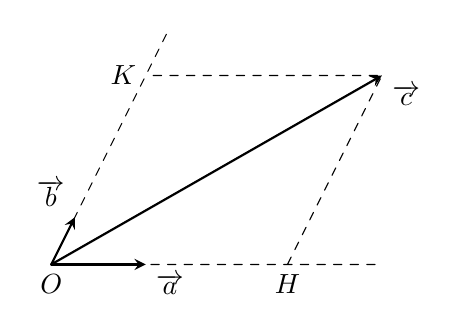
\begin{tikzpicture}[>=stealth,scale=0.6, line join=round, line cap=round]
		%\draw[line width=0.05pt,gray,dashed] (-0.7,-0.7) grid (8.7,4.7);
		\draw[->,thick](0,0)--(0.5,1)node[above left]{$\overrightarrow{b}$};
		\draw[->,thick](0,0)--(2,0)node[below right]{$\overrightarrow{a}$};
		\draw[->,thick](0,0)--(7,4)node[below right]{$\overrightarrow{c}$};
		\draw[dashed](0,0)--(7,0) (0,0)--(2.5,5) (5,0)--(7,4)--(2,4);
		\node[below] at (5,0) {$H$};
		\node[below] at (0,0) {$O$};
		\node[left] at (2,4) {$K$};
	\end{tikzpicture}}

\subsection{Các dạng toán}
\begin{dang}{Xác định vectơ tích, tính độ dài vectơ}%[Trần Quốc, BG10-2022, Nhóm 9]
	% vectơ $k\overrightarrow{a}$ có độ dài bằng $|k| |\overrightarrow{a}|$ và
	% \begin{enumEX}[$\bullet$]{2}
	% 	\item cùng hướng với $\overrightarrow{a}$ nếu $k \ge 0$;
	% 	\item ngược hướng với $\overrightarrow{a}$ nếu $\heva{&\overrightarrow{a}\ne \overrightarrow{0} \\ &k<0.}$
	% \end{enumEX}
\end{dang}
\subsubsection{Ví dụ minh họa}
\begin{vd}%[Trần Quốc, BG10-2022, Nhóm 9]%[0H1Y3-1]
	Cho đoạn thẳng $AB$ và $M$ là một điểm nằm trên đoạn $AB$ sao cho $AM=\dfrac{1}{5}AB$. Tìm $k$ trong các đẳng thức sau
	\begin{listEX}[3]
		\item $\overrightarrow{AM}=k\overrightarrow{AB}$.
		\item $\overrightarrow{MA}=k\overrightarrow{MB}$.
		\item $\overrightarrow{MA}=k\overrightarrow{AB}$.
	\end{listEX}
	\loigiai{
		\begin{center}
			\begin{tikzpicture}[font=\footnotesize,line join=round, line cap=round, >=stealth,scale=1.2]
				\tkzDefPoints{0/0/A, 5/0/B}
				\path ($(A)!1/5!(B)$) coordinate (M);
				\draw (A)--(B);
				\foreach \x in {0,...,5} \fill (\x,0) circle(1pt);
				\foreach \x in {A,M,B} \draw (\x) node[{shift=(-90:0.25)}]{$\x$};
			\end{tikzpicture}
		\end{center}
		\begin{listEX}[1]
			\item Thấy $\overrightarrow{AM}$ và $\overrightarrow{AB}$ cùng hướng nên $k>0$. \\
			Ta có $|k|=\dfrac{\left|\overrightarrow{AM}\right|}{\left|\overrightarrow{AB}\right|}=\dfrac{AM}{AB}=\dfrac{1}{5}$. Suy ra $k=\dfrac{1}{5}$.
			\item Thấy $\overrightarrow{MA}$ và $\overrightarrow{MB}$ ngược hướng nên $k<0$. \\
			Ta có $|k|=\dfrac{\left|\overrightarrow{MA}\right|}{\left|\overrightarrow{MB}\right|}=\dfrac{AM}{MB}=\dfrac{1}{4}$. Suy ra $k=-\dfrac{1}{4}$.
			\item Thấy $\overrightarrow{MA}$ và $\overrightarrow{AB}$ ngược hướng nên $k<0$. \\
			Ta có $|k|=\dfrac{\left|\overrightarrow{MA}\right|}{\left|\overrightarrow{AB}\right|}=\dfrac{AM}{AB}=\dfrac{1}{5}$. Suy ra $k=-\dfrac{1}{5}$.
		\end{listEX}}
\end{vd}

\begin{vd}%[Trần Quốc, BG10-2022, Nhóm 9]%[0H1B3-1]
	Cho tam giác $ABC$ đều cạnh bằng $1$, trọng tâm $G$. Tính độ dài vectơ $\overrightarrow{AG}$.
	\loigiai{
		\immini{Gọi $M$ là trung điểm của $BC$.\\
			Khi đó, ta có $\overrightarrow{AG}=\dfrac{2}{3}\overrightarrow{AM}$ nên
			\[\left|\overrightarrow{AG}\right|=\dfrac{2}{3}\left|\overrightarrow{AM}\right|=\dfrac{2}{3}AM=\dfrac{2}{3}\cdot\dfrac{\sqrt{3}}{2}=\dfrac{\sqrt{3}}{3}.\]}
		{\begin{tikzpicture}[font=\footnotesize,line join=round, line cap=round, >=stealth,scale=1]
				\tkzDefPoints{0/0/B, 4/0/C, 2/3.46/A}
				\path	 ($(B)!.5!(C)$) coordinate (M)
				($(A)!2/3!(M)$) coordinate (G);
				\draw (M)--(A)--(B)--(C)--(A);
				\foreach \x/\pos in {A/90,B/-150,C/-30,G/-160,M/-90} \fill (\x) circle(1pt) node[{shift=(\pos:0.25)}]{$\x$};
			\end{tikzpicture}}
	}
\end{vd}
\begin{vd}%[Trần Quốc, BG10-2022, Nhóm 9]%[0H1B3-1]
	Cho hình vuông $ABCD$ có cạnh bằng $a$, $I$ là trung điểm của cạnh $BC$. Tính độ dài vectơ $\overrightarrow{AB}+\overrightarrow{AC}$.
	\loigiai{
		\immini{
			Vì $I$ là trung điểm $BC$ nên ta có $\overrightarrow{AB}+\overrightarrow{AC}=2\overrightarrow{AI}$. \\
			Do đó $\left|\overrightarrow{AB}+\overrightarrow{AC}\right|=\left|2\overrightarrow{AI}\right|=2AI$.\\
			Xét $\triangle ABI$ vuông tại $B$, ta có $ AI=\sqrt{AB^2+BI^2}=\dfrac{a\sqrt{5}}{2} $.\\
			Vậy $ \left|\overrightarrow{AB}+\overrightarrow{AC}\right|=a\sqrt{5} $.}
		{
			\begin{tikzpicture}[line join = round, line cap = round,>=stealth,font=\footnotesize,scale=1]
				\tkzDefPoints{0/0/A}
				\coordinate (B) at ($(A)+(3,0)$);
				\tkzDefSquare(B,A)    \tkzGetPoints{D}{C}
				\coordinate (I) at ($(B)!1/2!(C)$);
				\draw (I)--(A)--(C)--(B)--(A)--(D)--(C);
				\foreach \x/\pos in {A/150, B/30, C/-30, D/-150, I/0} \fill (\x) circle(1pt) node[{shift=(\pos:0.25)}]{$\x$};
				\tkzMarkRightAngle(A,B,C);
			\end{tikzpicture}}

	}
\end{vd}
\subsubsection{Bài tập áp dụng}
\begin{bt}%[Trần Quốc, BG10-2022, Nhóm 9]%[0H1Y3-1]
	Trên đoạn thẳng $AB$, gọi $C$ là trung điểm $AB$ và $D$ là điểm đối xứng của $C$ qua $A$. Tìm $k$ trong các đẳng thức sau
	\begin{listEX}[2]
		\item $\overrightarrow{AC}=k\overrightarrow{AB}$.
		\item $\overrightarrow{AD}=k\overrightarrow{AB}$.
	\end{listEX}
	\loigiai{
		\begin{center}
			\begin{tikzpicture}[font=\footnotesize,line join=round, line cap=round, >=stealth,scale=1.2]
				\tkzDefPoints{0/0/A, 2/0/B}
				\path ($(A)!1/2!(B)$) coordinate (C)
				($(B)!3/2!(A)$) coordinate (D);
				\draw (D)--(B);
				\foreach \x in {-1,...,2} \fill (\x,0) circle(1pt);
				\foreach \x in {A,B,C,D} \draw (\x) node[{shift=(-90:0.25)}]{$\x$};
			\end{tikzpicture}
		\end{center}
		\begin{enumerate}
			\item Vì $C$ là trung điểm của $AB$ nên $\overrightarrow{AC}$ và $\overrightarrow{AB}$ cùng hướng. Do đó $k>0$.\\
			      Ta lại có $|k|=\dfrac{\left|\overrightarrow{AC}\right|}{\left|\overrightarrow{AB}\right|}=\dfrac{AC}{AB}=\dfrac{1}{2}$. Suy ra $k=\dfrac{1}{2}$.
			\item Vì $D$ đối xứng với $C$ qua $A$ nên $\overrightarrow{AD}$ và $\overrightarrow{AB}$ là ngược hướng, do đó $k<0$.\\
			      Ta lại có $AD=AC$ nên $|k|=\dfrac{\left|\overrightarrow{AD}\right|}{\left|\overrightarrow{AB}\right|}=\dfrac{AD}{AB}=\dfrac{AC}{AB}=\dfrac{1}{2}$. Suy ra $k=-\dfrac{1}{2}$.
		\end{enumerate}
	}
\end{bt}
\begin{bt}%[Trần Quốc, BG10-2022, Nhóm 9]%[0H1B3-1]
	Cho tam giác $ABC$ vuông cân tại $A$, cạnh $BC=2$. Gọi $M$, $N$ lần lượt là trung điểm của cạnh $AB$ và $BC$. Tính độ dài $\overrightarrow{MN}$.
	\loigiai{
		\immini{Vì $\triangle ABC$ vuông cân tại $A$ nên $AB^2=AC^2=\dfrac{1}{2}BC^2=2$, do đó $AB=AC=\sqrt{2}$.\\
			Dễ thấy rằng $MN$ là đường trung bình của $\triangle ABC$ nên $\overrightarrow{MN}=\dfrac{1}{2}\overrightarrow{AC}$.\\
			Suy ra $\left|\overrightarrow{MN}\right|=\dfrac{1}{2}\left|\overrightarrow{AC}\right|=\dfrac{1}{2}AC=\dfrac{\sqrt{2}}{2}$.
		}
		{\begin{tikzpicture}[font=\footnotesize,line join=round, line cap=round, >=stealth,scale=0.8]
				\tkzDefPoints{0/0/B, 5/0/C, 2.5/2.5/A}
				\path	 ($(A)!.5!(B)$) coordinate (M)
				($(B)!.5!(C)$) coordinate (N);
				\draw (M)--(N) (A)--(B)--(C)--(A);
				\foreach \x/\pos in {A/90,B/-150, C/-30, M/135, N/-90} \fill (\x) circle(1pt) node[{shift=(\pos:0.25)}]{$\x$};
				\tkzMarkRightAngle(B,A,C);
			\end{tikzpicture}}
	}
\end{bt}
\begin{bt}%[Trần Quốc, BG10-2022, Nhóm 9]%[0H1B3-1]
	Cho hình thoi $ABCD$ có $AC=2a$, $BD=a$. Tính độ dài vectơ $\overrightarrow{AC}+\overrightarrow{BD}$.
	\loigiai{
		\immini{
			Gọi $O$ là tâm của hình thoi.\\
			Khi đó ta có $\left|\overrightarrow{AC}+\overrightarrow{BD}\right|=\left|2\overrightarrow{AO}+2\overrightarrow{OD}\right|=\left|2\overrightarrow{AD}\right|=2AD$.\\
			Áp dụng định lý Pythagoras trong tam giác $AOD$ ta có $$AD=\sqrt{AO^2+OD^2}=\sqrt{a^2+\dfrac{a^2}{4}}=\dfrac{a\sqrt{5}}{2}.$$
			Do đó $\left|\overrightarrow{AC}+\overrightarrow{BD}\right|=2AD=a\sqrt{5}$.
		}
		{	\begin{tikzpicture}[scale=1, font=\footnotesize, line join=round, line cap=round, >=stealth]
				\def\r{2}
				\path
				(0:0) coordinate (B)
				(30:\r) coordinate (C)
				(90:\r) coordinate (D)
				(150:\r) coordinate (A)
				($(A)!0.5!(C)$) coordinate (O)
				;
				\draw (A)--(B)--(C)--(D)--(A)--(C) (B)--(D);
				\foreach \x/\pos in {A/-90,B/-90,C/-90,D/90,O/-45} \fill (\x) circle(1pt) node[{shift=(\pos:0.25)}]{$\x$};
				\tkzMarkRightAngle(D,O,A);
			\end{tikzpicture}
		}
	}
\end{bt}
\subsubsection{Bài tập trắc nghiệm}
\Opensolutionfile{ansbook}[ans/ansbook-0H1-3-1]
\Opensolutionfile{ans}[ans/ans-0H1-3-1]
\begin{ex}%[Trần Quốc, BG10-2022, Nhóm 9]%[0H1Y3-1]
	\immini[thm]{Cho hai vectơ  $\overrightarrow{AB}$ và $\overrightarrow{CD}$ trong hình bên. Khẳng định nào sau đây đúng?
		\choice
		{$\overrightarrow{CD}=3 \overrightarrow{AB}$}
		{$\overrightarrow{CD}=\overrightarrow{AB}$}
		{$\overrightarrow{AB}=2 \overrightarrow{CD}$}
		{\True $\overrightarrow{CD}=-3 \overrightarrow{AB}$}}
	{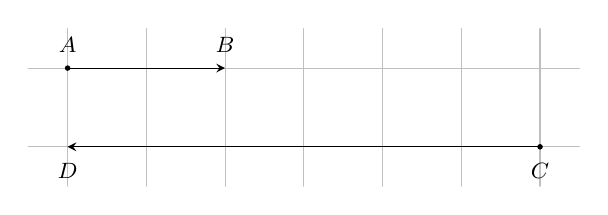
\begin{tikzpicture}[scale=1,font=\footnotesize,line join = round, line cap = round, >= stealth]
			\def\a{1}
			\draw[opacity=0.25] (-0.5,-0.5) grid (6.5,1.5);
			\coordinate (A) at (0,1);
			\coordinate (B) at (2,1);
			\coordinate (D) at (0,0);
			\coordinate (C) at (6,0);
			\draw[->] (A)--(B);
			\draw[->] (C)--(D);
			\foreach \p/\g in {A/90,B/90,C/-90,D/-90} \node at (\p) [shift={({\g}:.3)}]{$\p$};
			\foreach \x in {A,C} \fill (\x) circle(1pt);
		\end{tikzpicture}}
	\loigiai{
		Từ hình vẽ, theo định nghĩa ta có $\overrightarrow{CD}=-3 \overrightarrow{AB}$.
	}
\end{ex}
\begin{ex}%[Trần Quốc, BG10-2022, Nhóm 9]%[0H1Y3-1]
	Cho vectơ $\overrightarrow{a}$ (khác $\overrightarrow{0}$) và vectơ $\overrightarrow{b}=k\overrightarrow{a}$, $(k\ne 0)$. Khẳng định nào sau đây là đúng?
	\choice
	{$\overrightarrow{a}$ cùng phương $\overrightarrow{b}$ nếu $k>0$}
	{$\overrightarrow{a}$ ngược hướng $\overrightarrow{b}$ nếu $k>0$}
	{$\overrightarrow{a}$ cùng hướng $\overrightarrow{b}$ nếu $k<0$}
	{\True $\overrightarrow{a}$ cùng hướng $\overrightarrow{b}$ nếu $k>0$}
	\loigiai{
		vectơ $\overrightarrow{b}= k\overrightarrow{a}$ có độ dài bằng $|k| |\overrightarrow{a}|$ và
		\begin{itemize}
			\item cùng hướng với $\overrightarrow{a}$ nếu $k > 0$;
			\item ngược hướng với $\overrightarrow{a}$ nếu $k<0$.
		\end{itemize}
	}
\end{ex}
\begin{ex}%[Trần Quốc, BG10-2022, Nhóm 9]%[0H1Y3-1]
	Cho hai vectơ  $\vec{a}$, $\vec{b}$ bất kì và số thực $k$. Ta có $k\left(\vec{a}+\vec{b}\right)$ bằng
	\choice
	{$\vec{a}+k \vec{b}$}
	{\True $k \vec{a}+k \vec{b}$}
	{$k \vec{a}-k \vec{b}$}
	{$k \vec{a}+\vec{b}$}
	\loigiai{
		Theo tính chất, ta có $k(\vec{a}+\vec{b})=k \vec{a}+k \vec{b}$.
	}
\end{ex}
\begin{ex}%[Trần Quốc, BG10-2022, Nhóm 9]%[0H1Y3-1]
	Cho hai vectơ $\overrightarrow{a}$, $\overrightarrow{b}$ khác $\overrightarrow{0}$ thỏa mãn $\overrightarrow{a}=-\dfrac{1}{2}\overrightarrow{b}$. Mệnh đề nào dưới đây đúng?
	\choice
	{$\left|\overrightarrow{a}\right|=-\dfrac{1}{2}\left|\overrightarrow{b}\right|$}
	{$\overrightarrow{a}$ và $\overrightarrow{b}$ là hai vectơ đối nhau}
	{$\overrightarrow{a}$ cùng hướng với $\overrightarrow{b}$}
	{\True $\overrightarrow{a}$ ngược hướng với $\overrightarrow{b}$}
	\loigiai{
		Do $\overrightarrow{a}=-\dfrac{1}{2}\overrightarrow{b}$ và $-\dfrac{1}{2}<0$ nên $\overrightarrow{a}$ ngược hướng với $\overrightarrow{b}$.
	}
\end{ex}
\begin{ex}%[Trần Quốc, BG10-2022, Nhóm 9]%[0H1Y3-1]
	Cho vectơ $\overrightarrow{u}$ có độ dài bằng $2$ và vectơ $\overrightarrow{v}= -3\overrightarrow{u}$. Khẳng định nào sau đây là đúng?
	\choice
	{vectơ $\overrightarrow{v}$ có độ dài bằng $-6$ và cùng hướng với $\overrightarrow{u}$}
	{vectơ $\overrightarrow{v}$ có độ dài bằng $-6$ và ngược hướng với $\overrightarrow{u}$}
	{vectơ $\overrightarrow{v}$ có độ dài bằng $6$ và cùng hướng với $\overrightarrow{u}$}
	{\True vectơ $\overrightarrow{v}$ có độ dài bằng $6$ và ngược hướng với $\overrightarrow{u}$}
	\loigiai{Với $\overrightarrow{u}\ne \overrightarrow{0}$ và số thực $k\ne 0$, ta có
		$k\overrightarrow{u}$ ngược hướng với $\overrightarrow{u}$ nếu $k<0$ và $\left|k\overrightarrow{u}\right|=\left|k\right|\cdot \left|\overrightarrow{u}\right|$. \\
		Do đó, khẳng định đúng là: \lq\lq  vectơ $\overrightarrow{v}$ có độ dài bằng $6$ và ngược hướng với $\overrightarrow{u}$.\rq\rq
	}
\end{ex}
\begin{ex}%[Trần Quốc, BG10-2022, Nhóm 9]%[0H1Y3-1]
	Cho $\overrightarrow{a}=-2 \overrightarrow{b}$. Khẳng định nào sau đây đúng?
	\choice
	{\True $\overrightarrow{a}$ và $\overrightarrow{b}$ là hai vectơ bằng nhau}
	{$\overrightarrow{a}$ và $\overrightarrow{b}$ là hai vectơ đối nhau}
	{\True $\overrightarrow{a}$ và $\overrightarrow{b}$ ngược hướng}
	{$\overrightarrow{a}$ và $\overrightarrow{b}$ cùng hướng}
	\loigiai{
		Theo định nghĩa, nếu $\overrightarrow{a}=-2 \overrightarrow{b}$ thì $\overrightarrow{a}$ và $\overrightarrow{b}$ là hai vectơ ngược hướng.
	}
\end{ex}
% \begin{ex}%[Trần Quốc, BG10-2022, Nhóm 9]%[0H1Y3-1]
% 	Tích của vectơ $\overrightarrow{a}$ và $-3$ là vectơ $\overrightarrow{b}$. Khẳng định nào sau đây đúng?
% 	\choice
% 	{$\overrightarrow{b}$ cùng hướng $\overrightarrow{a}$}
% 	{$\overrightarrow{b}=3\overrightarrow{a}$}
% 	{$\left|\overrightarrow{b}\right|=-3\left|\overrightarrow{a}\right|$}
% 	{\True $\overrightarrow{b}$ ngược hướng $\overrightarrow{a}$}
% 	\loigiai{
% 		Theo giả thiết, ta có $\overrightarrow{b}=-3\overrightarrow{a}$ và $-3<0$ nên $\overrightarrow{b}$ ngược hướng $\overrightarrow{a}$.
% 	}
% \end{ex}
\begin{ex}%[Trần Quốc, BG10-2022, Nhóm 9]%[0H1Y3-1]
	Cho vectơ $\overrightarrow{q}$ có độ dài bằng $27$. Hỏi độ dài của vectơ $\overrightarrow{x}=-\dfrac{1}{9}\overrightarrow{q}$ là bao nhiêu?
	\choice
	{$243$}
	{\True $3$}
	{$9$}
	{$-3$}
	\loigiai{
		Ta có $\left| \overrightarrow{x} \right|=\dfrac{1}{9}\left| \overrightarrow{q} \right|=\dfrac{27}{9}=3$.
	}
\end{ex}
% \begin{ex}%[Trần Quốc, BG10-2022, Nhóm 9]%[0H1Y3-1]
% 	Cho vectơ $\overrightarrow{a}$ có độ dài bằng $2022$. Tính độ dài của vectơ $\overrightarrow{b}= -2\overrightarrow{a}$.
% 	\choice
% 	{\True $\left|\overrightarrow{b}\right|=4044$}
% 	{$\left|\overrightarrow{b}\right|=-2022$}
% 	{$\left|\overrightarrow{b}\right|=2022$}
% 	{$\left|\overrightarrow{b}\right|=-4044$}
% 	\loigiai{
% 		Ta có $\left|\overrightarrow{b}\right|=|-2\overrightarrow{a}|=2|\overrightarrow{a}|=2\cdot 2022=4044$.
% 	}
% \end{ex}
\begin{ex}%[Trần Quốc, BG10-2022, Nhóm 9]%[0H1Y3-1]
	\immini[thm]{Cho đoạn thẳng $AB$ và điểm $I$ thuộc đoạn thẳng $AB$ như hình vẽ bên. Mệnh đề nào sau đây đúng?
		\choice
		{$\overrightarrow{AI}=\dfrac{1}{4}\overrightarrow{AB}$}
		{\True $\overrightarrow{AI}=\dfrac{1}{4}\overrightarrow{IB}$}
		{$\overrightarrow{AI}=\dfrac{1}{5}\overrightarrow{BA}$}
		{$\overrightarrow{AI}=-\dfrac{1}{4}\overrightarrow{IB}$}}
	{    \begin{tikzpicture}[scale=1,font=\footnotesize,line join = round, line cap = round, >= stealth]
			\clip (-1,-1) rectangle (6,1);
			\tkzDefPoints{0/0/A, 5/0/B, 1/0/I}
			\draw (A)--(B);
			\foreach \x in {A,B,I} \fill (\x) circle(1pt) node[{shift=(90:0.25)}]{$\x$};
			\foreach \x in {2,3,4} \fill (\x,0) circle(1pt);
		\end{tikzpicture}}
	\loigiai{
		Từ hình vẽ ta có $\overrightarrow{AI}=\dfrac{1}{4}\overrightarrow{IB}$.
	}
\end{ex}
\begin{ex}%[Trần Quốc, BG10-2022, Nhóm 9]%[0H1Y3-1]
	\immini[thm]{
	Đẳng thức nào mô tả đúng hình vẽ bên?	
	\choice
		{\True $3\overrightarrow{AI}+\overrightarrow{AB}=\overrightarrow{0}$}
		{$3\overrightarrow{IA}+\overrightarrow{IB}=\overrightarrow{0}$}
		{$\overrightarrow{BI}+3\overrightarrow{BA}=\overrightarrow{0}$}
		{$\overrightarrow{AI}+3\overrightarrow{AB}=\overrightarrow{0}$}}
	{\begin{tikzpicture}[font=\footnotesize,line join = round, line cap = round,>=stealth,scale=1]
			\tkzDefPoints{0/0/A, 3/0/B, -1/0/I}
			\draw (I)--(B);
			\foreach \x in {I,A,B} \fill (\x) circle(1pt) node[{shift=(90:0.25)}]{$\x$};
			\fill (1,0) circle(1pt) (2,0) circle(1pt);
		\end{tikzpicture}}
	\loigiai{
		Từ hình vẽ ta thấy $\overrightarrow{IA}=\dfrac{1}{3}\overrightarrow{AB}\Leftrightarrow 3\overrightarrow{IA}=\overrightarrow{AB}\Leftrightarrow 3\overrightarrow{AI}+\overrightarrow{AB}=\overrightarrow{0}$.
	}
\end{ex}
\begin{ex}%[Trần Quốc, BG10-2022, Nhóm 9]%[0H1Y3-1]
	Cho $M$ là một điểm trên đoạn $AB$ sao cho $AM=\dfrac{1}{3} AB$. Khẳng định nào sau đây \textbf{sai}?
	\choice
	{\True $\overrightarrow{M B}=-\dfrac{2}{3} \overrightarrow{A B}$}
	{$\overrightarrow{A M}=\dfrac{1}{3} \overrightarrow{A B}$}
	{$\overrightarrow{M A}=-\dfrac{1}{2} \overrightarrow{M B}$}
	{$\overrightarrow{M B}=2 \overrightarrow{A M}$}
	\loigiai{
	\immini{
	Ta có $\overrightarrow{MB}$, $\overrightarrow{AB}$ cùng hướng và $MB=\dfrac{2}{3}AB$ nên $\overrightarrow{MB}=\dfrac{2}{3}\overrightarrow{AB}$.\\
	Khẳng định {\bf sai} là $\overrightarrow{M B}=-\dfrac{2}{3} \overrightarrow{A B}$.}
	{\begin{tikzpicture}[font=\footnotesize,line join=round, line cap=round, >=stealth,scale=1]
		\tkzDefPoints{0/0/A, 3/0/B, 1/0/M}
		\draw (A)--(B);
		\fill (2,0) circle(1pt);
		\foreach \x in {A,B,M} \fill (\x) circle(1pt) node[{shift=(90:0.25)}]{$\x$};
	\end{tikzpicture}}
	}
\end{ex}
\begin{ex}%[Trần Quốc, BG10-2022, Nhóm 9]%[0H1Y3-1]
	Cho đoạn thẳng $AB$ và $M$ là một điểm trên đoạn $AB$ sao cho $AB=5AM$. Mệnh đề nào sau đây \textbf{sai}?
	\choice
	{$\overrightarrow{MA}=-\dfrac{1}{4}\overrightarrow{MB}$}
	{$\overrightarrow{MB}=\dfrac{4}{5}\overrightarrow{AB}$}
	{\True $\overrightarrow{MB}=-\dfrac{4}{5}\overrightarrow{AB}$}
	{$\overrightarrow{AM}=\dfrac{1}{5}\overrightarrow{AB}$}
	\loigiai{
		\immini{
			Dễ thấy rằng $\overrightarrow{MB}$ và $\overrightarrow{AB}$ là hai vectơ cùng hướng nên mệnh đề sai là $\overrightarrow{MB}=-\dfrac{4}{5}\overrightarrow{AB}$.
		}
		{\begin{tikzpicture}[scale=0.8,>=stealth, font=\footnotesize, line join=round, line cap=round]
				\tkzDefPoints{0/0/A,5/0/B}
				\draw (A)--(B);
				\fill (0,0) node[above]{$A$} circle(1pt)
				(1,0)node[above]{$M$}circle(1pt)
				(2,0)circle(1pt)
				(3,0)circle(1pt)
				(4,0)circle(1pt)
				(5,0)node[above]{$B$}circle(1pt);
			\end{tikzpicture}}
	}
\end{ex}
\begin{ex}%[Trần Quốc, BG10-2022, Nhóm 9]%[0H1Y3-1]
	Cho đoạn thẳng $AB$, $M$ là một điểm trên đoạn thẳng $AB$ sao cho $AM=\dfrac{1}{4}AB$. Khẳng định nào sau đây {\bf sai}?
	\choice
	{$\overrightarrow{MA}=\dfrac{1}{3}\overrightarrow{MB}$}
	{$\overrightarrow{BM}=\dfrac{3}{4}\overrightarrow{BA}$}
	{\True $\overrightarrow{AM}=\dfrac{1}{4}\overrightarrow{AB}$}
	{$\overrightarrow{MB}=-3\overrightarrow{MA}$}
	\loigiai{
	\immini
	{
	Ta có $\overrightarrow{MA}$, $\overrightarrow{MB}$ ngược hướng và $MA=\dfrac{1}{3}MB$ nên $\overrightarrow{MA}=-\dfrac{1}{3}\overrightarrow{AB}$.\\
	Khẳng định {\bf sai} là $\overrightarrow{MA}=\dfrac{1}{3}\overrightarrow{MB}$.
	}
	{
	\begin{tikzpicture}[font=\footnotesize,line join=round, line cap=round, >=stealth,scale=1]
		\coordinate (A) at (0,0);
		\coordinate (B) at (4,0);
		\coordinate (M) at ($(A)!1/4!(B)$);
		\draw (A)--(B);
		\foreach \x in {A,B,M} \fill (\x) circle(1pt) node[{shift=(90:0.25)}]{$\x$};
		\foreach \x in {2,3} \fill (\x,0) circle(1pt);
	\end{tikzpicture}
	}
	}
\end{ex}
% \begin{ex}%[Trần Quốc, BG10-2022, Nhóm 9]%[0H1Y3-1]
% 	Trên đoạn thẳng $AB$ lấy điểm $I$ sao cho $AB=4AI$. Khẳng định nào sau đây là đúng?
% 	\choice
% 	{\True $\overrightarrow{IB}=-3\overrightarrow{IA}$}
% 	{$\overrightarrow{IB}=3\overrightarrow{IA}$}
% 	{$\overrightarrow{IB}=\dfrac{4}{3}\overrightarrow{AB}$}
% 	{$\overrightarrow{IB}=-\dfrac{3}{4}\overrightarrow{AB}$}
% 	\loigiai{
% 		\immini{
% 			Theo giả thiết ta có $IB=AB-AI=3AI$. \\
% 			Vì $\overrightarrow{IB}$ và $\overrightarrow{IA}$ ngược hướng nên $\overrightarrow{IB}=-3 \overrightarrow{I A}$.
% 		}{
% 			\begin{tikzpicture}[font=\footnotesize,line join=round, line cap=round, >=stealth,scale=1] 
% 				\coordinate (A) at (0,0);
% 				\coordinate (I) at (1,0);
% 				\coordinate (B) at (4,0);
% 				\draw (A)--(B);
% 				\foreach \x/\pos in {A/180, I/90, B/0} \fill (\x) circle(1pt) node[{shift=(\pos:0.25)}]{$\x$}; 
% 				\foreach \x in {2,3} \fill (\x,0) circle(1pt); 
% 			\end{tikzpicture}
% 		}
% 	}
% \end{ex}
% \begin{ex}%[Trần Quốc, BG10-2022, Nhóm 9]%[0H1Y3-1]
% 	Cho điểm $B$ nằm giữa hai điểm $A$ và $C$, với $AB=2a$, $AC=6a$. Đẳng thức nào dưới đây là đẳng thức đúng?
% 	\choice
% 	{\True $\overrightarrow{B C}=-2 \overrightarrow{B A}$}
% 	{$\overrightarrow{B C}=4 \overrightarrow{A B}$}
% 	{$\overrightarrow{B C}=-2 \overrightarrow{A B}$}
% 	{$\overrightarrow{B C}=-4 \overrightarrow{A B}$}
% 	\loigiai{
% 		\immini{
% 			Theo giả thiết ta có $BC=AC-AB=4a$. \\
% 			Vì $\overrightarrow{BA}$ và $\overrightarrow{BC}$ ngược hướng nên  $\overrightarrow{B C}=-2 \overrightarrow{B A}$.
% 		}{
% 			\begin{tikzpicture}[font=\footnotesize,line join=round, line cap=round, >=stealth,scale=1] 
% 				\coordinate (A) at (0,0);
% 				\coordinate (C) at (6,0);
% 				\coordinate (B) at (2,0);
% 				\draw (A)--(C);
% 				\foreach \x/\pos in {A/180, B/90, C/0} \fill (\x) circle(1pt) node[{shift=(\pos:0.25)}]{$\x$}; 
% 				\foreach \x in {1,3,4,5} \fill (\x,0) circle(1pt); 
% 			\end{tikzpicture}
% 		}
% 	}
% \end{ex}
\begin{ex}%[Trần Quốc, BG10-2022, Nhóm 9]%[0H1Y3-1]
	Cho hình bình hành $ABCD$ có tâm $O$. Mệnh đề nào sau đây \textbf{sai}?
	\choice
	{$\overrightarrow{OD}=\dfrac{1}{2}\overrightarrow{BD}$}
	{$\overrightarrow{AC}=2\overrightarrow{OC}$}
	{\True $\overrightarrow{AC}=2\overrightarrow{OA}$}
	{$\overrightarrow{AB}=\overrightarrow{DC}$}
	\loigiai{
		\immini{Ta có $\overrightarrow{AC}$ và $\overrightarrow{OA}$ là hai vectơ ngược hướng và $AC=2OA$ nên $\overrightarrow{AC}=2\overrightarrow{OA}$.}
		{\begin{tikzpicture}[line join = round, line cap = round,>=stealth,font=\footnotesize,scale=.6]
				\tkzDefPoints{0/0/D}
				\coordinate (C) at ($(D)+(5,0)$);
				\tkzDefShiftPoint[D](70:3){A}
				\coordinate (B) at ($(A)+(C)-(D)$);
				\coordinate (O) at ($(A)!0.5!(C)$);
				\pgfresetboundingbox
				\tkzDrawPolygon(A,B,C,D)
				\draw (A)--(C) (B)--(D);
				\foreach \x in {A,B,C,D,O} \fill (\x) circle(1pt);
				\tkzLabelPoints[above](A,B)
				\tkzLabelPoints[below](C,D,O)
			\end{tikzpicture}}
	}
\end{ex}
\begin{ex}%[Trần Quốc, BG10-2022, Nhóm 9]%[0H1B3-1]
	Cho tam giác $ABC$ với trung tuyến $AM$ và trọng tâm $G$. Khi đó, vectơ $\overrightarrow{GA}$ bằng với vectơ nào sau đây?
	\choice
	{$2\overrightarrow{GM}$}
	{\True $-\dfrac{2}{3}\overrightarrow{AM}$}
	{$\dfrac{2}{3}\overrightarrow{GM}$}
	{$\dfrac{1}{2}\overrightarrow{AM}$}
	\loigiai
	{
		\immini
		{Ta có $GA=\dfrac{2}{3}AM$ và $\overrightarrow{GA}$ ngược hướng $\overrightarrow{AM}$ nên $\overrightarrow{GA}=-\dfrac{2}{3}\overrightarrow{AM}$.}
		{\begin{tikzpicture}[line cap=round,line join=round,font=\footnotesize,>=stealth,scale=1]
				\fill (0:3) coordinate [label=right:$B$] (B) circle(1pt)
				(70:2) coordinate [label=above left:$C$] (C) circle(1pt)
				(0,0) coordinate [label=above left:$A$] (A) circle(1pt)
				($(C)!0.5!(B)$) coordinate [label=above right:$M$] (M) circle(1pt)
				($(A)!2/3!(M)$) coordinate [label=above left:$G$] (G) circle(1pt);
				\draw (A)--(B)--(C)--cycle (A)--(M);
			\end{tikzpicture}}
	}
\end{ex}
\begin{ex}%[Trần Quốc, BG10-2022, Nhóm 9]%[0H1B3-1]
	Cho tam giác $ABC$ có $G$ là trọng tâm, $M$ là trung điểm của $BC$. Đẳng thức nào sau đây đúng?
	\choice
	{\True $\overrightarrow{GB}+\overrightarrow{GC}=2\overrightarrow{GM}$}
	{$\overrightarrow{AB}+\overrightarrow{AC}=2\overrightarrow{AG}$}
	{$\overrightarrow{GA}=2\overrightarrow{GM}$}
	{$\overrightarrow{MG}=-\dfrac{1}{3}\overrightarrow{MA}$}
	\loigiai{
		\immini{Theo tính chất trung điểm ta có $\overrightarrow{GB}+\overrightarrow{GC}=2\overrightarrow{GM}$.}{\begin{tikzpicture}[scale=1, font=\footnotesize, line join=round, line cap=round, >=stealth]
				\tkzDefPoints{0/0/A, 4/0/B,1.5/3/C}
				\coordinate (M) at ($(B)!0.5!(C)$);
				\coordinate (G) at ($(A)!2/3!(M)$);
				\draw (A)--(B)--(C)--(A)--(M) (B)--(G)--(C);
				\foreach \x/\pos in {A/-150,B/-30,C/90,M/45,G/-90} \fill (\x) circle(1pt) node[{shift=(\pos:0.25)}]{$\x$};
			\end{tikzpicture}	}

	}
\end{ex}
\begin{ex}%[Trần Quốc, BG10-2022, Nhóm 9]%[0H1B3-1]
	Cho tam giác $ABC$. Gọi $M$, $N$ lần lượt là trung điểm của $AB$ và $AC$. Khẳng định nào sau đây là {\bf sai}?
	\choice
	{$\overrightarrow{MN}=\dfrac{1}{2}\overrightarrow{BC}$}
	{\True $\overrightarrow{MN}=-\dfrac{1}{2}\overrightarrow{BC}$}
	{$\overrightarrow{BC}=-2\overrightarrow{NM}$}
	{$\overrightarrow{BC}=2\overrightarrow{MN}$}
	\loigiai{
	\immini{
	Vì $M$, $N$ lần lượt là trung điểm của $AB$ và $AC$ nên $MN$ là đường trung bình của $\triangle ABC$. Do đó $MN \parallel BC$ và $MN =\dfrac{1}{2}BC$.\\
	Ta có các đẳng thức đúng là
	\begin{enumEX}[$\circ$]{3}
		\item $\overrightarrow{MN}=\dfrac{1}{2}\overrightarrow{BC}$.
		\item  $\overrightarrow{BC}=2\overrightarrow{MN}$.
		\item $\overrightarrow{BC}=-2\overrightarrow{NM}$.
	\end{enumEX}
	Đẳng thức $\overrightarrow{MN}=-\dfrac{1}{2}\overrightarrow{BC}$ là khẳng định {\bf sai}.
	}
	{
	\begin{tikzpicture}[font=\footnotesize,line join = round, line cap = round,>=stealth,scale=1]
		\path (1,3) coordinate (A)
		(0,0)  coordinate (B)
		(3,0)  coordinate (C)
		($(A)!.5!(B)$) coordinate (M)
		($(A)!.5!(C)$) coordinate (N)
		;
		\path
		(A) node [above]{$A$}
		(B) node [left]{$B$}
		(M) node [left]{$M$}
		(C) node [right]{$C$}
		(N) node [right]{$N$}
		;
		\foreach \x in {A,B,C,M,N} \fill[black] (\x) circle (1pt);
		\draw (A)--(B)--(C)--(A) (M)--(N);
	\end{tikzpicture}
	}
	}
\end{ex}
\begin{ex}%[Trần Quốc, BG10-2022, Nhóm 9]%[0H1B3-1]
	Cho tam giác $ABC$ có trọng tâm $G$ và trung tuyến $BM$. Khẳng định nào sau đây là {\bf sai}?
	\choice
	{$\overrightarrow{AM}=-\dfrac{1}{2}\overrightarrow{CA}$}
	{$\overrightarrow{GA}+\overrightarrow{GB}+\overrightarrow{GC}=\overrightarrow{0}$}
	{$\overrightarrow{OA}+\overrightarrow{OB}+\overrightarrow{OC}=3\overrightarrow{OG}$, với mọi điểm $O$}
	{\True $\overrightarrow{GB}=\dfrac{2}{3}\overrightarrow{BM}$}
	\loigiai{
		\immini{Do $\triangle ABC$ có trọng tâm $G$ và trung tuyến $BM$ nên ta có $BG=\dfrac{2}{3}BM$.\\
			Lại có $\overrightarrow{GB}$ và $\overrightarrow{BM}$ là hai vectơ ngược hướng nên $\overrightarrow{GB}=-\dfrac{2}{3}\overrightarrow{BM}$.\\
			Suy ra khẳng định sai là $\overrightarrow{GB}=\dfrac{2}{3}\overrightarrow{BM}$.}
		{\begin{tikzpicture}[font=\footnotesize,line join=round, line cap=round, >=stealth,scale=0.8]
				\tkzDefPoints{0/0/A, 1.5/2/B, 4/0/C}
				\path ($(A)!1/2!(C)$) coordinate (M)
				($(B)!2/3!(M)$) coordinate (G);
				\draw (M)--(B)--(A)--(C)--(B);
				\foreach \x/\pos in {A/-150, B/90, C/-30, M/-90, G/0} \fill (\x) circle(1pt) node[{shift=(\pos:0.25)}]{$\x$};
			\end{tikzpicture}}
	}
\end{ex}

\begin{ex}%[Trần Quốc, BG10-2022, Nhóm 9]%[0H1B3-1]
	Cho tam giác đều $ABC$ với đường cao $AH$. Mệnh đề nào sau đây đúng?
	\choice
	{$\overrightarrow{AB}=\overrightarrow{AC}$}
	{$\left|\overrightarrow{AH}\right|=\dfrac{\sqrt{3}}{2}\left|\overrightarrow{HC}\right|$}
	{$\overrightarrow{HB}=\overrightarrow{HC}$}
	{\True $\left|\overrightarrow{AC}\right|=2\left|\overrightarrow{HC}\right|$}
	\loigiai{
		\immini
		{
			Ta có $2\left|\overrightarrow{HC}\right|=\left|\overrightarrow{BC}\right|=BC=AC=\left|\overrightarrow{AC}\right|$.
		}
		{
			\begin{tikzpicture}[line join = round, line cap = round, scale=1]
				\def \a{2.5};
				\coordinate (B) at (0,0);
				\coordinate (C) at ($(B)+(\a,0)$);
				\coordinate[ shift=(60:\a cm)] (A) at (B);
				\coordinate (H) at ($(B)!0.5!(C)$);
				\draw (A)--(B)--(C)--cycle (A)--(H);
				\foreach \x in {A,B,C,H} \fill[black] (\x) circle (1.2pt);
				\tkzLabelPoints[below](H)
				\tkzLabelPoints[above](A)
				\tkzLabelPoints[left](B)
				\tkzLabelPoints[right](C)
			\end{tikzpicture}

		}
	}
\end{ex}

\begin{ex}%[Trần Quốc, BG10-2022, Nhóm 9]%[0H1Y3-1]
	Cho hình vuông $ABCD$ cạnh $a$. Giá trị của $\left|\overrightarrow{AB}+\overrightarrow{AC}+\overrightarrow{AD}\right|$ bằng
	\choice
	{$A\sqrt{2}$}
	{$ 2a$}
	{\True $ 2a\sqrt{2}$}
	{$ 3a$}
	\loigiai{\immini{
			Ta có $$\left|\overrightarrow{AB}+\overrightarrow{AC}+\overrightarrow{AD}\right|=\left|\overrightarrow{AC}+\overrightarrow{AC}\right|=2\left|\overrightarrow{AC}\right|=2AC=2a\sqrt{2}.$$}
		{\begin{tikzpicture}[scale=1, font=\footnotesize, line join=round, line cap=round, >=stealth]
				\def\a{2.5}
				\path
				(0:0) coordinate (A)
				(0:\a) coordinate (B)
				(-90:\a) coordinate (D)
				($(B)+(-90:\a)$) coordinate (C)
				;
				\draw (A)--(D)--(C)--(B)--(A)
				(A)--(C);
				\foreach \x/\pos in {A/90,B/90,C/-90,D/-90} \fill (\x) circle(1pt) node[{shift=(\pos:0.25)}]{$\x$};
			\end{tikzpicture}}
	}
\end{ex}
\begin{ex}%[Trần Quốc, BG10-2022, Nhóm 9]%[0H1B3-1]
	Cho tam giác $ABC$ đều cạnh $a$. Khi đó, giá trị $\left| \overrightarrow{AB}+\overrightarrow{AC}\right|$ bằng
	\choice
	{\True $a \sqrt{3}$}
	{$\dfrac{a \sqrt{3}}{2}$}
	{$2a$}
	{$\dfrac{a \sqrt{3}}{3}$}
	\loigiai{
		\immini{
			Gọi $M$ là trung điểm của $BC$. \\
			Vì $AM$ là đường trung tuyến của tam giác đều nên \[AM=\dfrac{\sqrt{3}}{2}\cdot a=\dfrac{a\sqrt{3}}{2}.\]
			Khi đó, ta có
			\[\left| \overrightarrow{AB}+\overrightarrow{AC}\right| = \left|2\overrightarrow{AM} \right| = 2\cdot AM = 2\cdot \dfrac{a\sqrt{3}}{2} = a\sqrt{3}.\]
		}{
			\begin{tikzpicture}[line cap=round,line join=round,>=stealth,scale=0.9,font=\footnotesize]
				\coordinate (B) at (0,0);
				\coordinate (C) at (4,0);
				\coordinate (A) at (2,3.46);
				\coordinate (M) at ($(B)!.5!(C)$);
				\draw (A)--(B)--(C)--(A)--(M);
				\foreach \x/\pos in {A/90, B/180, C/0, M/-90} \fill (\x) circle(1pt) node[{shift=(\pos:0.25)}]{$\x$};
			\end{tikzpicture}
		}
	}
\end{ex}
\begin{ex}%[Trần Quốc, BG10-2022, Nhóm 9]%[0H1B3-1]
	Cho tam giác đều $ABC$ cạnh bằng $4$. Độ dài $\overrightarrow{AB}+\overrightarrow{AC}$ là
	\choice
	{$ 2\sqrt{3}$}
	{$\sqrt{5}$}
	{$\sqrt{6}$}
	{\True $ 4\sqrt{3}$}
	\loigiai{\immini{
			Gọi $M$ là trung điểm của $BC$ .\\
			Vì $AM$ là đường trung tuyến của tam giác đều cạnh $4$ nên \[AM=\dfrac{\sqrt{3}}{2}\cdot 4=2\sqrt{3}.\]
			Do đó $\left|\overrightarrow{AB}+\overrightarrow{AC}\right|=\left|2\overrightarrow{AM}\right|=2AM=4\sqrt{3}$.
		}
		{	\begin{tikzpicture}[scale=0.8,>=stealth, font=\footnotesize, line join=round, line cap=round]
				\def\a{3.5}
				\pgfmathsetmacro{\y}{\a*(sqrt(3)/2)};
				\coordinate (A) at (0,0);
				\coordinate (B) at (\a,0);
				\coordinate (C) at (\a/2,\y);
				\coordinate (M) at ($(C)!0.5!(B)$);
				\draw(A)--(B)--(C)--cycle (A)--(M);
				\foreach \x/\pos in {A/-150, B/-30, C/90, M/30} \fill (\x) circle(1pt) node[{shift=(\pos:0.25)}]{$\x$};
				\tkzMarkRightAngle(A,M,B);
			\end{tikzpicture}}}
\end{ex}
\begin{ex}%[Trần Quốc, BG10-2022, Nhóm 9]%[0H1B3-1]
	Cho tam giác $ABC$ vuông tại $A$ và $AB=2$, $AC=3$. Độ dài của vectơ $\overrightarrow{BC}+\overrightarrow{AC}$ bằng
	\choice
	{$5$}
	{$40$}
	{$\sqrt{13}$}
	{\True $2\sqrt{10}$}
	\loigiai{
		\immini{Gọi $I$ là trung điểm của $AB$. Ta có \[\left|\overrightarrow{BC}+\overrightarrow{AC}\right|=\left|\overrightarrow{CB}+\overrightarrow{CA}\right|=\left|2\overrightarrow{CI}\right|=2CI.\]
			Tam giác $AIC$ vuông tại $A$ nên $CI=\sqrt{AI^2+AC^2}=\sqrt{1^2+3^2}=\sqrt{10}$.\\
			Vậy $\left|\overrightarrow{BC}+\overrightarrow{AC}\right|=2\sqrt{10}$.}{\begin{tikzpicture}[scale=1, font=\footnotesize, line join=round, line cap=round,>=stealth]
				\def\r{2};
				\path (180:\r)coordinate (B) (0:\r) coordinate (C) (120:\r) coordinate (A) ($(A)!0.5!(B)$) coordinate (I);
				\draw (A)--(B)--(C)--cycle (C)--(I);
				\foreach \p/\g in {A/90,B/-150,C/-30,I/135} \fill[black] (\p) circle(1pt)+(\g:0.3) node{$\p$};
				\tkzMarkRightAngle(B,A,C);
			\end{tikzpicture}}
	}
\end{ex}
\begin{ex}%[Trần Quốc, BG10-2022, Nhóm 9]%[0H1B3-1]
	Cho hình vuông $ ABCD $ có cạnh bằng $ a $. Tính $\left|\overrightarrow{AB}+\overrightarrow{DB}\right|$ theo $ a $.
	\choice
	{$\dfrac{a\sqrt 5}{2}$}
	{$a$}
	{\True $a\sqrt 5 $}
	{$a\sqrt 3 $}
	\loigiai{
		\immini{Gọi $ M $ là trung điểm của $ BC $.\\
			Ta có $\left|\overrightarrow{AB}+\overrightarrow{DB}\right| = \left|\overrightarrow{DC}+\overrightarrow{DB}\right| =2\left |\overrightarrow{DM}\right | =2\sqrt{a^2+\left(\dfrac{a}{2}\right )^2 } =a\sqrt{5}$. }{
			\begin{tikzpicture}[font=\footnotesize,line join=round, line cap=round, >=stealth,scale=0.8]
				\tkzDefPoints{0/0/A, 3/0/B, 3/3/C, 0/3/D};
				\coordinate (M) at ($ (B)!0.5!(C) $);
				\draw (A)--(B)--(C)--(D) --cycle (B)--(D)--(M);
				\foreach \x/\pos in {A/-90,B/-90,C/90,D/90,M/0} \fill (\x) circle(1pt) node[{shift=(\pos:0.25)}]{$\x$};
			\end{tikzpicture}}
	}
\end{ex}

\begin{ex}%[Trần Quốc, BG10-2022, Nhóm 9]%[0H1B3-1]
	\immini{Cho ba lực $\overrightarrow{F_1}=\overrightarrow{MA}$, $\overrightarrow{F_2}=\overrightarrow{MB}$, $\overrightarrow{F_3}=\overrightarrow{MC}$ cùng tác động vào một vật tại điểm $M$ và vật đứng yên. Cho biết cường độ của $\overrightarrow{F_1}$, $\overrightarrow{F_2}$ đều bằng $ 100$N và $\widehat{AMB}=60^\circ $. Khi đó, cường độ lực của $\overrightarrow{F_3}$ bằng
		\choice
		{$ 50\sqrt{2}$N}
		{$ 50\sqrt{3}$N}
		{$ 25\sqrt{3}$N}
		{\True $ 100\sqrt{3}$N} }{
		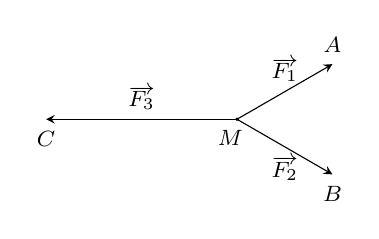
\begin{tikzpicture}[font=\footnotesize,line join=round, line cap=round, >=stealth,scale=0.7]
			\path
			(0:0) coordinate (M)
			(30:2) coordinate (A)
			(-30:2) coordinate (B)
			(180:{2*sqrt(3)}) coordinate (C);
			\draw[->] (M)--(A) node [pos=0.5, above] {$\overrightarrow{F_1}$};
			\draw[->] (M)--(B) node [pos=0.5, below] {$\overrightarrow{F_2}$};
			\draw[->] (M)--(C) node [pos=0.5, above] {$\overrightarrow{F_3}$};
			\fill (0,0) circle(1pt);
			\foreach \x/\pos in {M/-110, A/90, B/-90, C/-90} \node at (\x) [{shift=(\pos:0.25)}]{$\x$};
		\end{tikzpicture}
	}
	\loigiai{\immini{
			Gọi $D$ là đỉnh thứ tư của hình bình hành $MADB$ và $O$ là tâm hình bình hành.\\
			Khi đó, hợp lực  $\overrightarrow{F_1}+\overrightarrow{F_2}=\overrightarrow{MA}+\overrightarrow{MB}=\overrightarrow{MD}=2\overrightarrow{MO}$.\\
			Dễ thấy rằng $\triangle AMB$ là tam giác đều nên $MO=100\dfrac{\sqrt{3}}{2}$.\\
			Suy ra hợp lực $\overrightarrow{F_1}+\overrightarrow{F_2}$ có độ lớn $100\sqrt{3}$.\\
			Vì điểm $M$ đứng yên nên độ lớn của lực $\overrightarrow{F_3}$ là $100\sqrt{3} N$.
		}
		{\begin{tikzpicture}[font=\footnotesize,line join=round, line cap=round, >=stealth,scale=0.8]
				\path
				(0:0) coordinate (M)
				(30:2) coordinate (A)
				(-30:2) coordinate (B)
				(180:{2*sqrt(3)}) coordinate (C)
				($(A)+(B)$) coordinate (D)
				($(M)!1/2!(D)$) coordinate (O);
				\draw[->] (M)--(A) node [pos=0.5, above] {$\overrightarrow{F_1}$};
				\draw[->] (M)--(B) node [pos=0.5, below] {$\overrightarrow{F_2}$};
				\draw[->] (M)--(C) node [pos=0.5, above] {$\overrightarrow{F_3}$};
				\draw[->] (M)--(D);
				\draw[dashed,gray!70] (A)--(D)--(B)--(A);
				\fill (0,0) circle(1pt) (O) circle(1pt);
				\foreach \x/\pos in {M/-110, A/90, B/-90, C/-90, D/-30, O/-45} \node at (\x) [{shift=(\pos:0.25)}]{$\x$};
			\end{tikzpicture}}}
\end{ex}
\begin{ex}%[Trần Quốc, BG10-2022, Nhóm 9]%[0H1B3-1]
	Cho tam giác $ABC$ là tam giác đều cạnh $2a$ với $G$ là trọng tâm. Tính $\left| \overrightarrow{GB}+\overrightarrow{GC}\right|$.
	\choice
	{\True $\dfrac{2 a \sqrt{3}}{3}$}
	{$\dfrac{a \sqrt{3}}{2}$}
	{$\dfrac{a \sqrt{3}}{3}$}
	{$a \sqrt{3}$}
	\loigiai{
		\immini{
			Gọi $M$ là trung điểm của $BC$.\\
			Ta có $\left| \overrightarrow{GB}+\overrightarrow{GC}\right| = \left|2\overrightarrow{GM} \right| = 2\cdot GM = 2\cdot\dfrac{1}{3}\cdot AM=\dfrac{2}{3}\cdot\dfrac{2a\sqrt{3}}{2} = \dfrac{2a\sqrt{3}}{3}$.
		}{
			\begin{tikzpicture}[line cap=round,line join=round,>=stealth,scale=0.9,font=\footnotesize]
				\coordinate (B) at (0,0);
				\coordinate (C) at (4,0);
				\coordinate (A) at (2,3.46);
				\coordinate (M) at ($(B)!.5!(C)$);
				\coordinate (G) at ($(A)!.667!(M)$);
				\draw (A)--(B)--(C)--(A)--(M) (B)--(G)--(C);
				\foreach \x/\g in{A/90, B/180, C/0, M/-90, G/30}\fill[black](\x)circle(1pt)($(\x)+(\g:3mm)$)node{$\x$};
			\end{tikzpicture}
		}
	}
\end{ex}
\begin{ex}%[Trần Quốc, BG10-2022, Nhóm 9]%[0H1B3-1]
	Gọi $G$ là trọng tâm tam giác vuông $ABC$ với cạnh huyền $BC=12$. vectơ $\overrightarrow{GB}-\overrightarrow{CG}$ có độ dài bằng bao nhiêu?
	\choice
	{\True $4$}
	{$2\sqrt{3}$}
	{$8$}
	{$2$}
	\loigiai{
		\immini
		{
			Gọi $M$ là trung điểm của $BC$. \\
			Ta có $\overrightarrow{GB}-\overrightarrow{CG}=\overrightarrow{GB}+\overrightarrow{GC}=2\overrightarrow{GM}$.\\
			Vì $\triangle ABC$ vuông tại $A$ nên $AM=\dfrac{BC}{2}=6\Rightarrow GM=\dfrac{1}{3}AM=2$.\\
			Vậy $\left|\overrightarrow{GB}-\overrightarrow{CG}\right|=2\left|\overrightarrow{GM}\right|=2GM=4$.
		}
		{
			\begin{tikzpicture}[font=\footnotesize,line join=round, line cap=round, >=stealth,scale=0.8]
				\tkzDefPoints{-1/0/A, -2/-2/B, 2/-2/C};
				\coordinate (M) at ($(C)!1/2!(B)$);
				\coordinate (G) at ($(A)!2/3!(M)$);
				\draw (M)--(A)--(B)--(C)--(A) (B)--(G)--(C);
				\foreach \x/\pos in {A/90, B/-150, C/-30, M/-90, G/45} \fill (\x) circle(1pt) node[{shift=(\pos:0.25)}]{$\x$};
				\tkzMarkRightAngle(B,A,C);
			\end{tikzpicture}
		}
	}
\end{ex}
\begin{ex}%[Trần Quốc, BG10-2022, Nhóm 9]%[0H1B3-1]
	Tam giác $ABC$ có $AB=AC=a$, $\widehat{ABC}=120^\circ $. Độ dài vectơ tổng $\overrightarrow{AB}+\overrightarrow{AC}$ bằng
	\choice
	{$2a$}
	{$a\sqrt{3}$}
	{\True $a$}
	{$ 3a$}
	\loigiai{\immini{Gọi $M$ là trung điểm của $BC$, ta có $\overrightarrow{AB}+\overrightarrow{AC}=2\overrightarrow{AM}$.\\
			Tam giác $ABC$ cân tại $A$ có $\widehat{BAC}=120^\circ$ nên
			\[\widehat{ABM}=\dfrac{1}{2}\left(180^\circ-120^\circ\right)=30^\circ.\]
			Tam giác $ABM$ vuông tại $M$ có $\widehat{ABM}=30^\circ $ nên
			\[AM=AB\cdot \sin 30^\circ=\dfrac{a}{2}.\]
			Vậy $\left|\overrightarrow{AB}+\overrightarrow{AC}\right|=2\left|\overrightarrow{AM}\right|=2AM=a$. }
		{\begin{tikzpicture}[scale=0.8,>=stealth, font=\footnotesize, line join=round, line cap=round]
				\def\a{6}
				\pgfmathsetmacro{\y}{\a*(sqrt(3)/3)};
				\coordinate (B) at (0,0);
				\coordinate (C) at (\a,0);
				\coordinate (A) at (\a/2,\y/2);
				\coordinate (M) at ($(C)!0.5!(B)$);
				\filldraw (A) circle(1pt) node[above]{$A$};
				\filldraw (B) circle(1pt) node[below]{$B$};
				\filldraw (C) circle(1pt) node[below]{$C$};
				\filldraw (M) circle(1pt) node[below]{$M$};
				\draw(C)--(A)node[pos=.5,above]{$a$}--(B)node[pos=.5,above]{$a$}--(C)--cycle
				(A)--(M);
				\tkzMarkRightAngle(C,M,A)
				\tkzMarkAngle[size=0.5](M,B,A);
				\tkzLabelAngle[pos=1, font=\scriptsize](M,B,A){$30^\circ$}
			\end{tikzpicture}}}
\end{ex}

\begin{ex}%[Trần Quốc, BG10-2022, Nhóm 9]%[0H1B3-1]
	Cho hình thoi $ABCD$ cạnh $a$, tâm $O$ và $\widehat{BAD}=60^\circ$. Độ dài vectơ $\overrightarrow{OB}-\overrightarrow{CD}$ bằng
	\choice
	{\True $\dfrac{a\sqrt{7}}{2}$}
	{$\dfrac{a\sqrt{5}}{2}$}
	{$2a$}
	{$a\sqrt{3}$}
	\loigiai{
		\immini{
			Gọi $G$ là trung điểm của đoạn $OC$.\\
			Ta có $\left|\overrightarrow{OB}-\overrightarrow{CD}\right|=\left|\overrightarrow{DO}+\overrightarrow{DC}\right|=2\left|\overrightarrow{DG}\right|=2DG$.\\
			Tam giác $DOG$ vuông tại $O$ có $DO=\dfrac{a}{2}$, $OG=\dfrac{OC}{2}=\dfrac{a\sqrt{3}}{4}$ nên
			$$DG=\sqrt{DO^2+OG^2}=\sqrt{\left(\dfrac{a}{2}\right)^2+\left(\dfrac{a\sqrt{3}}{4}\right)^2}=\dfrac{a\sqrt{7}}{4}.$$
			Suy ra $\left|\overrightarrow{OB}-\overrightarrow{CD}\right|=2\cdot \dfrac{a\sqrt{7}}{4}=\dfrac{a\sqrt{7}}{2}$.
		}{
			\begin{tikzpicture}[scale=1, font=\footnotesize, line join=round, line cap=round, >=stealth]
				\def\r{2}
				\path
				(0:0) coordinate (B)
				(30:\r) coordinate (C)
				(90:\r) coordinate (D)
				(150:\r) coordinate (A)
				($(A)!0.5!(C)$) coordinate (O)
				($(O)!0.5!(C)$) coordinate (G)
				;
				\draw (A)--(B)--(C)--(D)--(A)--(C) (B)--(D)--(G);
				\foreach \x/\g in {A/-135,B/-90,C/-30,D/90,O/-135, G/-90}
				\fill (\x) circle(1pt) ($(\x)+(\g:0.25)$) node{$\x$};
			\end{tikzpicture}
		}
	}
\end{ex}

\begin{ex}%[Trần Quốc, BG10-2022, Nhóm 9]%[0H1B3-1]
	Cho tam giác $ABC$ đều cạnh $a$, $H$ là trung điểm của $BC$. Tính $\left|\overrightarrow{CA}-\overrightarrow{HC}\right|$ bằng
	\choice
	{$\dfrac{2\sqrt{3}a}{3}$}
	{\True $\dfrac{a\sqrt{7}}{2}$}
	{$\dfrac{a}{2}$}
	{$\dfrac{3a}{2}$}
	\loigiai{\immini{
			Gọi $K$ là trung điểm của $AH$. Khi đó
			\[\left|\overrightarrow{CA}-\overrightarrow{HC}\right|=\left|\overrightarrow{CA}+\overrightarrow{CH}\right|=\left|2\overrightarrow{CK}\right|=2CK.\]
			Xét $\triangle KHC$ vuông tại $H$ có $HC=\dfrac{a}{2}$, $KH=\dfrac{1}{2}AH=\dfrac{a\sqrt{3}}{4}$. Do đó
			$$CK=\sqrt{CH^2+HK^2}=\sqrt{\left(\dfrac{a}{2}\right)^2+\left(\dfrac{a\sqrt{3}}{4}\right)^2}=\dfrac{a\sqrt{7}}{4}.$$
			Vậy $\left|\overrightarrow{CA}-\overrightarrow{HC}\right|=\dfrac{a\sqrt{7}}{4}$.
		}{\begin{tikzpicture}[scale=0.8,>=stealth, font=\footnotesize, line join=round, line cap=round]
				\def\a{3.5}
				\pgfmathsetmacro{\y}{\a*(sqrt(3)/2)};
				\coordinate (A) at (0,0);
				\coordinate (B) at (\a,0);
				\coordinate (C) at (\a/2,\y);
				\coordinate (H) at ($(C)!0.5!(B)$);
				\coordinate (K) at ($(A)!0.5!(H)$);
				\draw (A)--(B)--(C)--(K) (A)--(C) (A)--(H);
				\foreach \x/\pos in {A/-150, B/-30, C/90, H/45, K/-75} \fill (\x) circle(1pt) node[{shift=(\pos:0.25)}]{$\x$};
				\tkzMarkRightAngle(A,H,C);
			\end{tikzpicture}}}
\end{ex}
\begin{ex}%[Trần Quốc, BG10-2022, Nhóm 9]%[0H1B3-1]
	Cho tam giác $OAB$ vuông cân tại $O$ với $OA=OB=a$. Tính độ dài vectơ $\overrightarrow{u}=8\overrightarrow{OA}-6\overrightarrow{OB}$.
	\choice
	{$2a$}
	{$14a$}
	{$16a$}
	{\True $10a$}
	\loigiai{
		\immini
		{
			Lấy điểm $M$ sao cho $\overrightarrow{OM}=8\overrightarrow{OA}$. Khi đó
			\[OM=\left|\overrightarrow{OM}\right|=\left|8\overrightarrow{OA}\right|=8OA=8a.\]
			Lấy điểm $N$ sao cho $\overrightarrow{ON}=6\overrightarrow{OB}$. Khi đó
			\[ON=\left|\overrightarrow{ON}\right|=\left|6\overrightarrow{OB}\right|=6OB=6a.\]
			Vì $OA\perp OB$ nên $OM\perp ON$, hay $\triangle OMN$ vuông tại $O$. Do đó
			\begin{align*}
				\left|\overrightarrow{u}\right| & =\left|8\overrightarrow{OA}-6\overrightarrow{OB}\right|=\left|\overrightarrow{OM}-\overrightarrow{ON}\right| \\
				                                & =\left|\overrightarrow{NM}\right|=MN=\sqrt{OM^2+ON^2}                                                        \\
				                                & =\sqrt{(8a)^2+(6a)^2}=10a.
			\end{align*}
		}
		{
			\begin{tikzpicture}[font=\footnotesize,line join=round, line cap=round, >=stealth,scale=1]
				\tkzDefPoints{0/0/O,0.5/0/B,0/0.5/A,3/0/N,0/4/M}
				\draw (A)--(B)--(O)--(M)--(N)--(B);
				\foreach \x/\pos in {O/-150, A/180, B/-90, M/150, N/-30} \fill (\x) circle(1pt) node[{shift=(\pos:0.25)}]{$\x$};
			\end{tikzpicture}
		}
	}
\end{ex}
\begin{ex}%[Trần Quốc, BG10-2022, Nhóm 9]%[0H1B3-1]
	Cho tam giác $ABC$ vuông tại $A$ có $AB=3$, $AC=4$. Tính độ dài vec-tơ $\overrightarrow{u}=2\overrightarrow{AB}+3\overrightarrow{AC}$.
	\choice
	{$\left|\overrightarrow{u}\right|=18$}
	{\True $\left|\overrightarrow{u}\right|=6\sqrt{5}$}
	{$\left|\overrightarrow{u}\right|=9$}
	{$\left|\overrightarrow{u}\right|=5\sqrt{6}$}
	\loigiai{
		\immini{
			Gọi $D$, $E$ là hai điểm thỏa $\overrightarrow{AD}=2\overrightarrow{AB}$ và $\overrightarrow{AE}=3\overrightarrow{AC}$. \\
			Suy ra $AD=6$, $AE=12$.\\
			Gọi $F$ là điểm sao cho tứ giác $ADFE$ là hình chữ nhật.\\
			Suy ra $AF=\sqrt{AD^2+AE^2}=\sqrt{6^2+12^2}=6\sqrt{5}$.\\
			Ta có
			$$\overrightarrow{u}=2\overrightarrow{AB}+3\overrightarrow{AC}=\overrightarrow{AD}+\overrightarrow{AE}=\overrightarrow{AF}.$$
			Suy ra $\left|\overrightarrow{u}\right|=\left|\overrightarrow{AF}\right|=6\sqrt{5}$.}
		{\begin{tikzpicture}[font=\footnotesize,line join=round, line cap=round, >=stealth,scale=0.7]
				\tkzDefPoints{0/0/A, 1.5/0/B, 0/2/C}
				\path ($(A)!2!(B)$) coordinate (D)
				($(A)!3!(C)$) coordinate (E)
				($(E)+(D)-(A)$) coordinate (F);
				\draw (A)--(E)--(F)--(D)--(A)--(F) (B)--(C);
				\foreach \x/\pos in {A/-150, B/-90, C/180, D/-30, E/150, F/30} \fill (\x) circle(1pt) node[{shift=(\pos:0.25)}]{$\x$};
				\fill (0,4) circle(1pt);
			\end{tikzpicture}}
	}
\end{ex}
\begin{ex}%[Trần Quốc, BG10-2022, Nhóm 9]%[0H1B3-1]
	Gọi $ G $	 là trọng tâm của tam giác $ ABC $. Tập hợp điểm $ M $ trong mặt phẳng chứa tam giác $ ABC $ sao cho $ \left| \overrightarrow{MA} + \overrightarrow{MB}+ \overrightarrow{MC}\right|=6$ là
	\choice
	{đường tròn ngoại tiếp tam giác $ ABC $}
	{đường tròn tâm $ G $ bán kính bằng $ 1 $}
	{\True đường tròn tâm $ G $ bán kính bằng $ 2 $}
	{đường tròn tâm $ G $ bán kính bằng $ 6 $}
	\loigiai{
		Ta có $G$ là trọng tâm $\triangle ABC$ nên $\overrightarrow{MA} + \overrightarrow{MB}+ \overrightarrow{MC}=3\overrightarrow{MG}$. \\
		Do đó $\left|3\overrightarrow{MG}\right|=6 \Leftrightarrow MG=2$.\\
		Vậy tập hợp điểm $ M $ là đường tròn tâm $ G $ bán kính bằng $ 2 $.
	}
\end{ex}
\begin{ex}%[Trần Quốc, BG10-2022, Nhóm 9]%[0H1K3-1]
	Cho tam giác đều $ABC$ có cạnh bằng $2a$ và $G$ là trọng tâm của tam giác. Khi đó, giá trị $\left|\overrightarrow{AB}-\overrightarrow{GC}\right|$ là
	\choice
	{$\dfrac{a\sqrt{3}}{3}$}
	{$\dfrac{2a\sqrt{3}}{3}$}
	{\True $\dfrac{4a\sqrt{3}}{3}$}
	{$\dfrac{2a}{3}$}
	\loigiai{
		\immini{
			Vì $G$ là trọng tâm của $\triangle ABC$ nên ta có $\overrightarrow{GA}+\overrightarrow{GB}+\overrightarrow{GC}=\overrightarrow{0}$.\\
			Do đó
			\[\left|\overrightarrow{AB}-\overrightarrow{GC}\right|=\left|\overrightarrow{GB}-\overrightarrow{GA}-\overrightarrow{GC}\right|=\left|\overrightarrow{GB}+\overrightarrow{GB}\right|=\left|2\overrightarrow{GB}\right|=2GB.\]
			Gọi $M$ là trung điểm $AC$. Khi đó
			\[GB=\dfrac{2}{3}BM=\dfrac{2}{3}\cdot 2a\cdot\dfrac{\sqrt{3}}{2}=\dfrac{2a\sqrt{3}}{3}.\]
			Suy ra
			$\left|\overrightarrow{AB}-\overrightarrow{GC}\right|=2\cdot\dfrac{2a\sqrt{3}}{3}=\dfrac{4a\sqrt{3}}{3}$.
		}{\begin{tikzpicture}[scale=1, font=\footnotesize, line join=round, line cap=round,>=stealth]
				\path (0,0)coordinate (B)
				(3,0) coordinate (C)
				($(B)!1!60:(C)$) coordinate (A)
				($(A)!0.5!(C)$) coordinate (M)
				($(B)!2/3!(M)$) coordinate (G) ;
				\draw (A)--(B)--(C)--cycle (B)--(M);
				\foreach \x/\pos in {A/90,B/-150,C/-30,G/135, M/30} \fill (\x) circle(1pt) node[{shift=(\pos:0.25)}]{$\x$};
			\end{tikzpicture}}
	}
\end{ex}
\begin{ex}%[Trần Quốc, BG10-2022, Nhóm 9]%[0H1K3-1]
	Cho ba lực $\vec{F}_1$, $\vec{F}_2$, $\vec{F}_3$ có cùng điểm đặt tại $O$. Trong đó, có hai lực $\vec{F}_1$, $\vec{F}_2$ có phương hợp với nhau một góc $90^\circ$ và lực $\vec{F}_3$ ngược hướng với lực $\vec{F}_1$. Ba lực $\vec{F}_1$, $\vec{F}_2$, $\vec{F}_3$ có cường độ lần lượt là $100$ N, $200$ N và $300$ N. Cường độ lực tổng hợp của ba lực $\vec{F}_1$, $\vec{F}_2$, $\vec{F}_3$ là
	\choice
	{$400$ N}
	{$100\sqrt{2}$ N}
	{$600$ N}
	{\True $200\sqrt{2}$ N}
	\loigiai{
	\immini{
	Gọi $\vec{F}_{13}=\vec{F}_1+\vec{F}_3$.\\
	Vì $\vec{F}_1$ ngược hướng với $\vec{F}_3$ nên $F_{13}=|F_1-F_3|=200$ N.\\
	Suy ra $\vec{F}=\vec{F}_1+\vec{F}_2+\vec{F}_3=\vec{F}_{13}+\vec{F}_2$.\\
	Do $\vec{F}_2\perp\vec{F}_{13}$, suy ra $F=\sqrt{F_2^2+F_{13}^2}=\sqrt{200^2+200^2}=200\sqrt{2}$ N.
	}{
	\begin{tikzpicture}[font=\footnotesize,line join=round, line cap=round, >=stealth,scale=0.8]
		\def\r{1}
		\path (0,0)coordinate(O)+(0:\r)coordinate(A)+(90:2*\r)coordinate(B)+(180:3*\r)coordinate(C) (180:\r)coordinate(D) ($(D)+(B)-(O)$)coordinate(E);
		\draw[->] (O)--(B)node[above right]{$\vec{F}_2$};
		\draw[->] (O)--(C)node[below]{$\vec{F}_3$};
		\draw[->] (O)--(D)node[below]{$\vec{F}_{13}$};
		\draw[->] (O)--(A)node[below]{$\vec{F}_1$};
		\draw[->] (O)--(E)node[above left]{$\vec{F}$};
		\fill (0,0) circle(1pt) node[shift=(-90:0.25)]{$O$};
		\draw[dashed] (B)--(E)--(D);
	\end{tikzpicture}
	}
	}
\end{ex}
\begin{ex}%[Trần Quốc, BG10-2022, Nhóm 9]%[0H1K3-1]
	Cho hình vuông $ABCD$ có cạnh bằng $1$. Độ dài của vectơ $\overrightarrow{u}=12\overrightarrow{AC}-7\overrightarrow{AB}$ bằng
	\choice
	{$\left|\overrightarrow{u}\right|=17$}
	{\True $\left|\overrightarrow{u}\right|=5$}
	{$\left|\overrightarrow{u}\right|=13$}
	{$\left|\overrightarrow{u}\right|=12\sqrt{2}-7$}
	\loigiai{
	\immini{Gọi $O$, $M$, $N$ lần lượt là tâm của hình vuông $ABCD$, trung điểm của đoạn $AD$, trung điểm của đoạn $DM$. Ta có
	{\allowdisplaybreaks
	\begin{eqnarray*}
		12\overrightarrow{AC}-7\overrightarrow{AB} & = & 6\overrightarrow{AO}-6\overrightarrow{AB}-\overrightarrow{AB}=6\overrightarrow{BO}-\overrightarrow{AB}\\
		& = & 3\overrightarrow{BD}+\overrightarrow{BA}=2\overrightarrow{BD}+\left(\overrightarrow{BD}+ \overrightarrow{BA}\right)\\
		& = & 2\overrightarrow{BD} + 2 \overrightarrow{BM} = 2 \left(\overrightarrow{BD} +  \overrightarrow{BM}\right)\\
		& = & 2 \cdot 2 \overrightarrow{BN} = 4 \overrightarrow{BN}.
	\end{eqnarray*}}Do đó $\left|\overrightarrow{u}\right|=4 BN$.\\
	Xét $\triangle ABN$ vuông tại $A$, có
	$BN=\sqrt{AB^2+AN^2}=\sqrt{1^2+\left(\dfrac{3}{4}\right)^2}=\dfrac{5}{4}.$\\
	Vậy $\left|\overrightarrow{u}\right|=4 \cdot \dfrac{5}{4} =5$.
	}{
	\begin{tikzpicture}[>=stealth,line join=round, line cap=round, font=\footnotesize, scale=0.8]
		\path
		(0,0) coordinate (A)
		(4,0) coordinate (B)
		(4,-4) coordinate (C)
		($(A)+(C)-(B)$) coordinate (D)
		($(A)!1/2!(C)$) coordinate (O)
		($(A)!1/2!(D)$) coordinate (M)
		($(D)!1/2!(M)$) coordinate (N)
		;
		\draw (A)--(B)--(C)--(D)--(A)--(C) (B)--(D) (B)--(M) (B)--(N);
		\foreach \x/\pos in {A/135,B/45,C/-45,D/-135,O/-90,M/180,N/180} \fill (\x) circle(1pt) node[{shift=(\pos:0.25)}]{$\x$};
	\end{tikzpicture}}
	}
\end{ex}
\begin{ex}%[Trần Quốc, BG10-2022, Nhóm 9]%[0H1K3-1]
	Cho hình vuông $ABCD$ có cạnh bằng $1$. Độ dài của vectơ $\overrightarrow{u}=3\overrightarrow{AC}-7\overrightarrow{AB}$ là
	\choice
	{\True $|\overrightarrow{u}|=5$}
	{$|\overrightarrow{u}|=12\sqrt{2}-7$}
	{$|\overrightarrow{u}|=17$}
	{$|\overrightarrow{u}|=13$}
	\loigiai{
		\immini{Ta có $\overrightarrow{u}=3\left(\overrightarrow{AB}+\overrightarrow{AD}\right)-7\overrightarrow{AB}=-4\overrightarrow{AB}+3\overrightarrow{AD}$.\\
			Dựng $E$, $F$, $G$ sao cho $\overrightarrow{AE}=-4\overrightarrow{AB}$,  $\overrightarrow{AF}=3\overrightarrow{AD}$ và $AEGF$ là hình bình hành.\\
			Vì $AB\perp AD$ nên $AE\perp AF$. Do đó $AEGF$ là hình chữ nhật.\\
			Vậy $\overrightarrow{u}=\overrightarrow{AG}$ và
			$\left|\overrightarrow{u}\right|=\left|\overrightarrow{AG}\right|=AG=EF=\sqrt{AE^2+AF^2}=\sqrt{4^2+3^2}=5$.}
		{\begin{tikzpicture}[scale=1, font=\footnotesize, line join=round, line cap=round,>=stealth]
				\path (0,0)coordinate (B)
				(1,0) coordinate (C)
				($(B)!1!90:(C)$) coordinate (A)
				($(A)+(C)-(B)$) coordinate (D)
				($(A)!-4!(B)$) coordinate (E)
				($(A)!3!(D)$) coordinate (F)
				($(E)+(F)-(A)$) coordinate (G);
				\draw (A)--(B)--(C)--(D)--cycle;
				\draw[->] (A)--(E);
				\draw[->] (A)--(F);
				\draw[->] (A)--(G);
				\draw[dashed] (E)--(G)--(F);
				\foreach \x/\pos in {A/180,B/-150,C/-30,D/60,E/150,F/0,G/30} \fill (\x) circle(1pt) node[{shift=(\pos:0.25)}]{$\x$};
			\end{tikzpicture}}
	}
\end{ex}

\Closesolutionfile{ans}
\Closesolutionfile{ansbook}
% % \indapan{10}{ans/ans-0H1-3-1}




\begin{dang}%[Huỳnh Đức Vũ, BG10-2022, Nhóm 9]
	{Chứng minh đẳng thức vectơ, thu gọn biểu thức}
	\textbf{\textit{Phương pháp giải}}
	\begin{itemize}
		\item Cách 1: Biến đổi thẳng VT về VP hoặc ngược lại.
		\item Cách 2: Biến đổi VT và VP về cùng bằng một biểu thức trung gian.
		\item Cách 3: Chứng minh VT-VT=$\vec{0}$.
	\end{itemize}
	\textit{\textbf{Khi thực hiện các phép biến đổi cần lưu ý}}
	\begin{enumerate}
		\item \textit{Quy tắc ba điểm:} Với ba điểm $A$, $B$, $C$ bất kì ta luôn có
		      $ \overrightarrow {AB}= \overrightarrow {AC}  +  \overrightarrow{CB}$.
		\item \textit{Quy tắc hình bình hành:} Với hình bình hành $ABCD$ ta luôn có
		      $ \overrightarrow {AC}= \overrightarrow {AB}  +  \overrightarrow{A D}$.
		\item \textit{Quy tắc hiệu vectơ:} Với ba điểm $A$, $B$, $O$ bất kì ta luôn có
		      $ \overrightarrow {OB} -  \overrightarrow{OA}= \overrightarrow {AB}$.
		\item \textit{Tính chất trung điểm của đoạn thẳng:} Cho đoạn thẳng $AB$ ta
		      có
		      \allowdisplaybreaks
		      \begin{eqnarray*}
			      I\;\text{là trung điểm của}\;AB&\Leftrightarrow&
			      \overrightarrow {IA} + \overrightarrow{IB}= \overrightarrow {0}\\
			      &\Leftrightarrow&
			      \overrightarrow {MA}  +  \overrightarrow{MB}=2\overrightarrow{MI}, M \;\text{là điểm bất kì}.
		      \end{eqnarray*}
		\item \textit{Tính chất trọng tâm tam giác:} Cho tam giác $ABC$ ta có
		      \allowdisplaybreaks
		      \begin{eqnarray*}
			      G\;\text{là trọng tâm tam giác}\; ABC &\Leftrightarrow&
			      \overrightarrow {GA}  +  \overrightarrow{GB}  +  \overrightarrow{GC}= \overrightarrow {0}.\\
			      &\Leftrightarrow& \overrightarrow {MA}  +  \overrightarrow{MB}  +  \overrightarrow{MC}=3 \overrightarrow {MG}, M\;\text{là điểm bất kì }.
		      \end{eqnarray*}
		\item \textit{Các tính chất của phép cộng, trừ vectơ và phép nhân một số với một vectơ.}
	\end{enumerate}
\end{dang}
\subsubsection{Ví dụ minh họa}
\begin{vd}%[Huỳnh Đức Vũ, BG10-2022, Nhóm 9]%[0H1B3-2]
	Cho tam giác $ABC$ với trọng tâm $G$. Chứng minh rằng $ \overrightarrow {CA}  +  \overrightarrow{CB}= 3 \overrightarrow {CG}$.
	\loigiai{ \immini{
			Gọi $K$ là trung điểm của $AB$ thì $\overrightarrow {CA}  +  \overrightarrow{CB} =2\overrightarrow {CK}$.\qquad(1)\\
			Vì $G$ là trọng tâm của tam giác $ABC$ nên
			$\overrightarrow {CG} =\dfrac{2}{3}\overrightarrow {CK}$, tức là $3\overrightarrow {CG}=2\overrightarrow {CK}$.\qquad (2)\\
			Từ $(1)$ và $(2)$ ta có $ \overrightarrow {CA}  +  \overrightarrow{CB}= 3 \overrightarrow {CG}$.
		}{\begin{tikzpicture}[scale=1, font=\footnotesize, line join=round, line cap=round, >=stealth]
				\path
				(0,0) coordinate (A)
				(4,0) coordinate (B)
				(2,3) coordinate (C)
				($(B)!.5!(C)$) coordinate (P)
				($(A)!.5!(C)$) coordinate (N)	($(A)!2/3!(P)$) coordinate (G)
				($(A)!0.5!(B)$) coordinate (K)
				;
				\foreach \x/\y in {C/K,B/C,P/A,A/C,A/B,B/N}
				\draw (\x)--(\y);
				\foreach \x/\g in {A/180,B/0,C/90,G/180,K/-90} \fill[black] (\x) circle (1pt)+(\g:0.4) node{$\x$};
			\end{tikzpicture}}}
\end{vd}
\begin{vd}%[Huỳnh Đức Vũ, BG10-2022, Nhóm 9]%[0H1B3-2]
	Cho hình bình hành $ABCD$. Gọi $G$ là trọng tâm tam giác $ABD$. Chứng minh rằng \[ \overrightarrow {AB}  +   \overrightarrow {2AC}  +  \overrightarrow{AD}=9\overrightarrow {AG}.\]
	\loigiai{\immini{
			Vì $ABCD$ là hình bình hành nên ta có $ \overrightarrow {AB}  +  \overrightarrow{AD}= \overrightarrow {AC}$.\\
			Suy ra
			\allowdisplaybreaks
			\begin{eqnarray*}
				\overrightarrow {AB}  +  2 \overrightarrow {AC}  +  \overrightarrow{AD}  &=&  \left( \overrightarrow {AB}  +  \overrightarrow{AD}\right)  +  2 \overrightarrow {AC}\\
				& =&  \overrightarrow{AC}  +  2 \overrightarrow {AC}=3 \overrightarrow {AC}. \qquad(1)
			\end{eqnarray*}
		}{\begin{tikzpicture}[scale=1, font=\footnotesize, line join=round, line cap=round, >=stealth]
				\path
				(3,2) coordinate(D)
				(2,0) coordinate(C)
				(-1,0) coordinate(B);
				\coordinate (A) at ($(D)+(B)-(C)$)
				($(A)!1/2!(C)$) coordinate (O)
				($(A)!2/3!(O)$) coordinate (G)
				($(A)!1/2!(B)$) coordinate (M);
				\draw (B)--(D)--(C)--(B)--(A)--(D)
				(A)--(C) (D)--(M);
				\foreach \x/\g in {A/90,O/-90,G/90,B/-90,C/-90, D/90}
				\fill[black] (\x) circle(1pt) ($(\x)+(\g:3mm)$) node{$\x$};
			\end{tikzpicture}}Gọi $O$ là tâm hình bình hành $ABCD$.\\ Vì $G$ là trọng tâm tam giác $ABD$ nên ta có $\overrightarrow {AG}=\dfrac{2}{3}\overrightarrow {AO}=\dfrac{1}{3}\overrightarrow {AC}$. Suy ra $\overrightarrow {AC}=3\overrightarrow {AG}$.\qquad (2)\\
		Từ $(1)$ và $(2)$ ta có $\overrightarrow {AB}  +   \overrightarrow {2AC}  +  \overrightarrow{AD}=9\overrightarrow {AG}$.}
\end{vd}
\begin{vd}%[Huỳnh Đức Vũ, BG10-2022, Nhóm 9]%[0H1B3-2]
	Cho tứ giác $ABCD$. Gọi $M$ và $N$ lần lượt là trung điểm các đoạn thẳng $AB$ và $CD$. Chứng minh rằng
	$ \overrightarrow {AC} + \overrightarrow{BD}=2 \overrightarrow {MN}$.
	\loigiai{
		\immini{
			\textit{Cách 1.} Ta có
			\begin{eqnarray*}
				\overrightarrow {AC}= \overrightarrow {AM} + \overrightarrow{MN} + \overrightarrow {NC}, \\
				\overrightarrow {BD}= \overrightarrow {BM} + \overrightarrow {MN} + \overrightarrow {ND}.
			\end{eqnarray*}
			Cộng hai đẳng thức trên theo vế ta được:
			\begin{eqnarray*}
				\overrightarrow {AC}  +  \overrightarrow{BD}  &=&  2 \overrightarrow {MN}  +  \left( \overrightarrow {AM}  +  \overrightarrow{BM}\right)  +  \left( \overrightarrow {NC}  +  \overrightarrow{ND}\right)\\
				&=&  2 \overrightarrow {MN}.
			\end{eqnarray*}
			(Vì $ \overrightarrow {AM} + \overrightarrow {BM}=  \overrightarrow{0}$ và $ \overrightarrow {NC}+ \overrightarrow {ND}= \overrightarrow{0}$).
		}
		{
			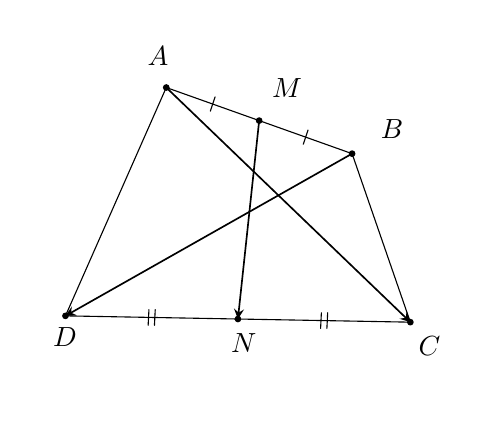
\begin{tikzpicture}[line cap=round,line join=round,>=stealth,x=1.0cm,y=1.0cm,scale=1]
				\clip(1.62,-0.62) rectangle (7.1,4.02);
				\draw (3.38,3.26)-- (2.1,0.36);
				\draw (6.48,0.28)-- (5.74,2.42);
				\draw [->,line width=0.6pt] (4.56,2.84) -- (4.29,0.32);
				\draw [->,line width=0.6pt] (3.38,3.26) -- (6.48,0.28);
				\draw [->,line width=0.6pt] (5.74,2.42) -- (2.1,0.36);
				\draw (3.02,3.9) node[anchor=north west] {$A$};
				\draw (5.98,2.98) node[anchor=north west] {$B$};
				\draw (6.46,0.22) node[anchor=north west] {$C$};
				\draw (1.82,0.34) node[anchor=north west] {$D$};
				\draw (4.6,3.5) node[anchor=north west] {$M$};
				\draw (4.08,0.26) node[anchor=north west] {$N$};
				\draw (4.56,2.84)-- (3.38,3.26);
				\draw (3.94,2.96) -- (4.0,3.14);
				\draw (4.56,2.84)-- (5.74,2.42);
				\draw (5.18,2.72) -- (5.12,2.54);
				\draw (2.1,0.36)-- (4.29,0.32);
				\draw (3.16,0.44) -- (3.15,0.24);
				\draw (3.24,0.44) -- (3.23,0.24);
				\draw (4.29,0.32)-- (6.48,0.28);
				\draw (5.35,0.4) -- (5.34,0.2);
				\draw (5.43,0.4) -- (5.42,0.2);
				\begin{scriptsize}
					\draw [fill=black] (3.38,3.26) circle (1pt);
					\draw [fill=black] (2.1,0.36) circle (1pt);
					\draw [fill=black] (6.48,0.28) circle (1pt);
					\draw [fill=black] (5.74,2.42) circle (1pt);
					\draw [fill=black] (4.56,2.84) circle (1pt);
					\draw [fill=black] (4.29,0.32) circle (1pt);
				\end{scriptsize}
			\end{tikzpicture}
		}
		\noindent\textit{Cách 2.} Ta có
		\begin{eqnarray*}
			&&\overrightarrow {MN}= \overrightarrow {MA}  +  \overrightarrow{AC}  +  \overrightarrow{CN},\\
			&&\overrightarrow {MN}= \overrightarrow {MB}  +  \overrightarrow{BD}  +  \overrightarrow{DN}.
		\end{eqnarray*}
		Cộng hai đẳng thức trên theo vế ta được
		\allowdisplaybreaks
		\begin{eqnarray*}
			2 \overrightarrow {MN}  &=&  \left( \overrightarrow {AM}  +  \overrightarrow{BM}\right)  +  \left( \overrightarrow {NC}  +  \overrightarrow{ND}\right)  +  \overrightarrow{AC}  +  \overrightarrow{BD} \\
			&=&  \overrightarrow{AC}  +  \overrightarrow{BD}.
		\end{eqnarray*}
		(Vì $ \overrightarrow {AM} + \overrightarrow {BM}=  \overrightarrow{0}$ và $ \overrightarrow {NC}+ \overrightarrow {ND}= \overrightarrow{0}$).\\
		\begin{note} Ta cũng có đẳng thức
			$ \overrightarrow {AD} + \overrightarrow{BC}=2 \overrightarrow {MN}$. Học sinh chứng minh tương tự.
		\end{note}

	}
\end{vd}

\begin{vd}%[Huỳnh Đức Vũ, BG10-2022, Nhóm 9]%[0H1K3-2]
	Cho tam giác $ABC$. Lần lượt lấy các điểm $M$, $N$, $P$ trên các đoạn thẳng $AB$, $BC$ và $CA$ sao cho $AM=\dfrac{1}{3}AB$, $BN=\dfrac{1}{3}BC$, $CP=\dfrac{1}{3}CA$. Chứng minh rằng
	\[ \overrightarrow {AN}  +  \overrightarrow{BP}  +  \overrightarrow{CM}= \overrightarrow {0}.\]
	\loigiai{
		\immini{
			Ta có
			\allowdisplaybreaks
			\begin{eqnarray}
				&& \overrightarrow{BN}=\dfrac{1}{3} \overrightarrow {BC}\Leftrightarrow \overrightarrow{AN}  -  \overrightarrow{AB}=\dfrac{1}{3} \overrightarrow {BC}. \\
				&& \overrightarrow{CP}=\dfrac{1}{3} \overrightarrow {CA}\Leftrightarrow \overrightarrow{BP}  -  \overrightarrow{BC}=\dfrac{1}{3} \overrightarrow {CA}. \\
				&& \overrightarrow{AM}=\dfrac{1}{3} \overrightarrow {AB}\Leftrightarrow \overrightarrow{CM}  -  \overrightarrow{CA}=\dfrac{1}{3} \overrightarrow {AB}.
			\end{eqnarray}
		}
		{
			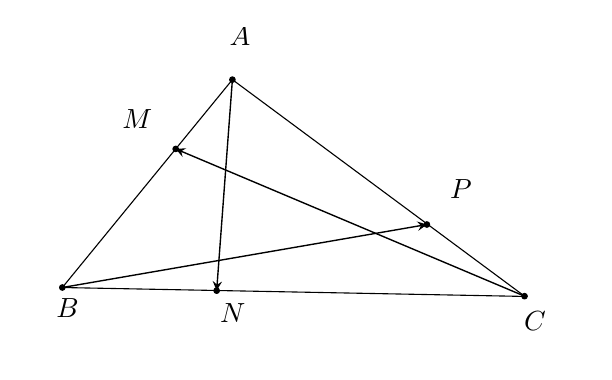
\begin{tikzpicture}[line cap=round,line join=round,>=stealth,x=1.0cm,y=1.0cm,scale=1]
				\clip(0.16,-0.36) rectangle (7.22,3.76);
				\draw (0.6,0.46)-- (6.468006178401337,0.346749903462479);
				\draw (2.76,3.1)-- (0.6,0.46);
				\draw (2.76,3.1)-- (6.47,0.35);
				\draw (2.6,3.9) node[anchor=north west] {$A$};
				\draw (0.4,0.44) node[anchor=north west] {$B$};
				\draw (6.34,0.28) node[anchor=north west] {$C$};
				\draw (1.24,2.84) node[anchor=north west] {$M$};
				\draw (2.48,0.38) node[anchor=north west] {$N$};
				\draw (5.4,1.96) node[anchor=north west] {$P$};
				\draw [->,line width=0.5pt] (2.76,3.1) -- (2.56,0.42);
				\draw [->,line width=0.5pt] (0.6,0.46) -- (5.23,1.26);
				\draw [->,line width=0.5pt] (6.47,0.35) -- (2.04,2.22);
				\begin{scriptsize}
					\draw [fill=black] (0.6,0.46) circle (1pt);
					\draw [fill=black] (2.04,2.22) circle (1pt);
					\draw [fill=black] (2.76,3.1) circle (1pt);
					\draw [fill=black] (5.23,1.26) circle (1pt);
					\draw [fill=black] (6.47,0.35) circle (1pt);
					\draw [fill=black] (2.56,0.42) circle (1pt);
				\end{scriptsize}
			\end{tikzpicture}
		}
		Từ $(1)$, $(2)$ và $(3)$ ta suy ra
		\allowdisplaybreaks
		\begin{eqnarray*}
			&& \overrightarrow{AN}  +  \overrightarrow{BP}  +  \overrightarrow{CM}  -  \left( \overrightarrow {AB}  +  \overrightarrow{BC}  +  \overrightarrow{CA}\right)=\dfrac{1}{3}\left( \overrightarrow {AB}  +  \overrightarrow{BC}  +  \overrightarrow{CA}\right) \\
			& \Leftrightarrow& \overrightarrow{AN}  +  \overrightarrow{BP}  +  \overrightarrow{CM}=\dfrac{4}{3}\left( \overrightarrow {AB}  +  \overrightarrow{BC}  +  \overrightarrow{CA}\right)\\
			&\Leftrightarrow& \overrightarrow{AN}  +  \overrightarrow{BP}  +  \overrightarrow{CM}=\dfrac{4}{3} \overrightarrow {0}\\
			&\Leftrightarrow& \overrightarrow{AN}  +  \overrightarrow{BP}  +  \overrightarrow{CM}=\overrightarrow {0}.
		\end{eqnarray*}
	}
\end{vd}
\begin{vd}%[Huỳnh Đức Vũ, BG10-2022, Nhóm 9]%[0H1K3-2]
	Cho hình bình hành $ABCD$ có tâm $O$. Gọi $M$ là một điểm bất kì. Chứng minh rằng
	\begin{enumerate}
		\item $ \overrightarrow {OA}  +  \overrightarrow{OB}  +  \overrightarrow{OC}  +  \overrightarrow{OD}= \overrightarrow {0}$.
		\item $ \overrightarrow {MA}  +  \overrightarrow{MB}  +  \overrightarrow{MC}  +  \overrightarrow{MD}=4 \overrightarrow {MO}$.
	\end{enumerate}
	\loigiai {\begin{enumerate}
			\item Chứng minh $ \overrightarrow {OA}  +  \overrightarrow{OB}  +  \overrightarrow{OC}  +  \overrightarrow{OD}= \overrightarrow {0}$.
			      \immini{
				      Vì $O$ là trung điểm của $AC$ và $BD$ nên ta có
				      \begin{eqnarray*}
					      \allowdisplaybreaks
					      && \overrightarrow{OA}  +  \overrightarrow{OC}= \overrightarrow {0}, \\
					      && \overrightarrow{OB}  +  \overrightarrow{OD}= \overrightarrow {0}.
				      \end{eqnarray*}
				      Do đó $ \overrightarrow {OA}  +  \overrightarrow{OB}  +  \overrightarrow{OC}  +  \overrightarrow{OD}= \overrightarrow {0}$.}
			      {\begin{tikzpicture}[scale=1, font=\footnotesize, line join=round, line cap=round, >=stealth]
					      \path
					      (3,2) coordinate(D)
					      (2,0) coordinate(C)
					      (-1,0) coordinate(B);
					      \coordinate (A) at ($(D)+(B)-(C)$)
					      ($(A)!1/2!(C)$) coordinate (O)
					      ($(A)!1/2!(B)$) coordinate (M);
					      \draw (B)--(D)--(C)--(B)--(A)--(D)
					      (A)--(C);
					      \foreach \x/\g in {A/90,O/-90,B/-90,C/-90, D/90}
					      \fill[black] (\x) circle(1pt) ($(\x)+(\g:3mm)$) node{$\x$};
				      \end{tikzpicture}}
			\item Theo quy tắc ba điểm ta có
			      \allowdisplaybreaks
			      \begin{eqnarray*}
				      && \overrightarrow{MA}= \overrightarrow {MO}  +  \overrightarrow{OA}, \\
				      && \overrightarrow{MB}= \overrightarrow {MO}  +  \overrightarrow{OB}, \\
				      && \overrightarrow{MC}= \overrightarrow {MO}  +  \overrightarrow{OC}, \\
				      && \overrightarrow{MD}= \overrightarrow {MO}  +  \overrightarrow{OD}.
			      \end{eqnarray*}
			      Suy ra $ \overrightarrow {MA}  +  \overrightarrow{MB}  +  \overrightarrow{MC}  +  \overrightarrow{MD}=4 \overrightarrow {MO}  +  \left( \overrightarrow {OA}  +  \overrightarrow{OB}  +  \overrightarrow{OC}  +  \overrightarrow{OD}\right)$. \\
			      Theo ý $a)$ ta có $ \overrightarrow {OA}  +  \overrightarrow{OB}  +  \overrightarrow{OC}  +  \overrightarrow{OD}= \overrightarrow {0}$.\\
			      Vậy $ \overrightarrow {MA}  +  \overrightarrow{MB}  +  \overrightarrow{MC}  +  \overrightarrow{MD}=4 \overrightarrow {MO}$ với $M$ là điểm bất kì.
		\end{enumerate}
	}
\end{vd}
\begin{vd}%[Huỳnh Đức Vũ, BG10-2022, Nhóm 9]%[0H1K3-2]
	Cho hình bình hành $ABCD$. Gọi $M$ là trung điểm $CD$. Lấy $N$ trên đoạn $BM$ sao cho $BN = 2MN$. Chứng minh rằng
	\begin{enumerate}
		\item  $3\overrightarrow{AB} + 4\overrightarrow{CD}= \overrightarrow{CM} + \overrightarrow{ND} + \overrightarrow{MN}$,
		\item  $ 4\overrightarrow{AB} + 2\overrightarrow{BD}=3\overrightarrow{AN}$.
	\end{enumerate}
	\loigiai{
		\begin{center}
			\begin{tikzpicture}[line join = round, line cap = round,>=stealth,font=\footnotesize,scale=1]
				\tkzDefPoints{0/0/D}
				\coordinate (C) at ($(D)+(5,0)$);
				\tkzDefShiftPoint[D](70:3){A}
				\coordinate (B) at ($(A)+(C)-(D)$);
				\pgfresetboundingbox
				\coordinate (M) at ($(D)!0.5!(C)$);
				\draw (A)--(B) (B)--(C) (D)--(C)--(A)--(D)-- (B)--(M);
				\coordinate (O) at ($(A)!0.5!(C)$);
				\coordinate (N) at ($(B)!2/3!(M)$);
				\tkzDrawPoints[fill=black](A,B,C,D,M,N,O)
				\tkzLabelPoints[above](A,B,N,O)
				%\tkzLabelPoints[left](E)
				\tkzLabelPoints[below](C,D,M)
			\end{tikzpicture}
		\end{center}
		\begin{enumerate}
			\item Ta có
			      \allowdisplaybreaks
			      \begin{eqnarray*}
				      &&VT = 3\overrightarrow{AB} + 4\overrightarrow{CD} = 3(\overrightarrow{AB} + \overrightarrow{CD}) + \overrightarrow{CD} = \overrightarrow{CD}.\qquad(1)\\
				      &&VP = \overrightarrow{CM} + \overrightarrow{MN}+ \overrightarrow{ND} = \overrightarrow{CD}. \qquad(2)
			      \end{eqnarray*}
			      Từ $(1)$ và $(2)$ suy ra $VT = VP$.
			\item Ta có $N$ thuộc đoạn $BM$ và $BN = 2MN$ nên $N$ là trọng tâm của tam giác $BCD$.\\ Ta có
			      \allowdisplaybreaks
			      \begin{eqnarray*}
				      VP&=&3\overrightarrow{AN}= \overrightarrow{AB}+\overrightarrow{AD}+\overrightarrow{AC}=2\overrightarrow{AC}.\\
				      VT&=&4\overrightarrow{AB} + 2\overrightarrow{BD} \\
				      &=& 2\overrightarrow{AB} + 2(\overrightarrow{AB} + \overrightarrow{BD})\\
				      &=& 2\overrightarrow{AB} + 2\overrightarrow{AD} \\
				      &=& 2\overrightarrow{AB} + 2\overrightarrow{BC} \\
				      &=& 2\left(\overrightarrow{AB} + \overrightarrow{BC}\right) = 2 \overrightarrow{AC}.
			      \end{eqnarray*}
			      Vậy $ 4\overrightarrow{AB} + 2\overrightarrow{BD}=3\overrightarrow{AN}$
		\end{enumerate}}
\end{vd}

\subsubsection{Bài tập áp dụng}

\begin{bt}%[Huỳnh Đức Vũ, BG10-2022, Nhóm 9]%[0H1B3]
	Cho hình bình hành $ABCD$ có tâm $O$. Chứng minh rằng \[ \overrightarrow {BA}  +  \overrightarrow{BC}  +  \overrightarrow{BD}=4 \overrightarrow {OD}.\]
	\loigiai{
		\immini{
			Ta có
			$$ \overrightarrow {BA}  +  \overrightarrow{BC}  +  \overrightarrow{BD}=2 \overrightarrow {BD}=4 \overrightarrow {OD}.$$
		}{\begin{tikzpicture}[scale=1, font=\footnotesize, line join=round, line cap=round, >=stealth]
				\path
				(3,2) coordinate(D)
				(2,0) coordinate(C)
				(-1,0) coordinate(B);
				\coordinate (A) at ($(D)+(B)-(C)$)
				($(A)!1/2!(C)$) coordinate (O)
				($(A)!1/2!(B)$) coordinate (M);
				\draw (B)--(D)--(C)--(B)--(A)--(D)
				(A)--(C);
				\foreach \x/\g in {A/90,O/-90,B/-90,C/-90, D/90}
				\fill[black] (\x) circle(1pt) ($(\x)+(\g:3mm)$) node{$\x$};
			\end{tikzpicture}}}
\end{bt}
\begin{bt}%[Huỳnh Đức Vũ, BG10-2022, Nhóm 9]%[0H1K3]
	Gọi $G$ và $G'$ lần lượt là trọng tâm của tam giác $ABC$ và $A'B'C'$. Chứng minh rằng
	\[ \overrightarrow {AA'}  +  \overrightarrow{BB'}  +  \overrightarrow{CC'}=3 \overrightarrow {GG'}.\]
	\loigiai{
		Áp dụng quy tắc ba điểm, ta có
		\begin{eqnarray*}
			&& \overrightarrow{AA'}= \overrightarrow {AG}  +  \overrightarrow{GG'}  +  \overrightarrow{GA'}, \\
			&& \overrightarrow{BB'}= \overrightarrow {BG}  +  \overrightarrow{GG'}  +  \overrightarrow{GB'}, \\
			&& \overrightarrow{CC'}= \overrightarrow {CG}  +  \overrightarrow{GG'}  +  \overrightarrow{GC'}.
		\end{eqnarray*}
		Suy ra $ \overrightarrow {AA'}  +  \overrightarrow{BB'}  +  \overrightarrow{CC'}=3 \overrightarrow {GG'}  +  \left( \overrightarrow {AG}  +  \overrightarrow{BG}  +  \overrightarrow{CG}\right)  +  \left( \overrightarrow {GA'}  +  \overrightarrow{GB'}  +  \overrightarrow{GC'}\right).$\\
		Vì $G$ và $G'$ lần lượt là trọng tâm của tam giác $ABC$ và $A'B'C'$ nên ta có
		\begin{eqnarray*}
			&& \overrightarrow{AG}  +  \overrightarrow{BG}  +  \overrightarrow{CG}= \overrightarrow {0}, \\
			&& \overrightarrow{GA'}  +  \overrightarrow{GB'}  +  \overrightarrow{GC'}=\overrightarrow {0}.
		\end{eqnarray*}
		Vậy $ \overrightarrow {AA'}  +  \overrightarrow{BB'}  +  \overrightarrow{CC'}=3 \overrightarrow {GG'}$.
	}
\end{bt}
\begin{bt}%[Huỳnh Đức Vũ, BG10-2022, Nhóm 9]%[0H1K3]
	Cho tứ giác $ABCD$. Gọi $M$, $N$, $I$ lần lượt là trung điểm của $AC$, $BD$ và $MN$. Chứng minh rằng
	\begin{enumerate}
		\item $ \overrightarrow {IA}  +  \overrightarrow{IB}  +  \overrightarrow{IC}  +  \overrightarrow{ID}= \overrightarrow {0}$,
		\item $ \overrightarrow {OA}  +  \overrightarrow{OB}  +  \overrightarrow{OC}  +  \overrightarrow{OD}=4 \overrightarrow {OI}$ (với $O$ là điểm bất kì).
	\end{enumerate}

	\loigiai{
		\immini{
			a) Vì $M,N$ lần lượt là trung điểm của $AC$ và $BD$ nên ta có\\
			\begin{eqnarray*}
				&& \overrightarrow{IA}  +  \overrightarrow{IC}=2 \overrightarrow {IM}, \\
				&& \overrightarrow{IB}  +  \overrightarrow{ID}=2 \overrightarrow {IN}.
			\end{eqnarray*}
			Suy ra
			\begin{eqnarray*}
				\overrightarrow {IA}  +  \overrightarrow{IB}  +  \overrightarrow{IC}  +  \overrightarrow{ID}  &=&  \left( \overrightarrow {IA}  +  \overrightarrow{IC}\right)  +  \left( \overrightarrow {IB}  +  \overrightarrow{ID}\right) \\
				&=&2\left( \overrightarrow {IM}  +  \overrightarrow{IN}\right).
			\end{eqnarray*}
		}
		{
			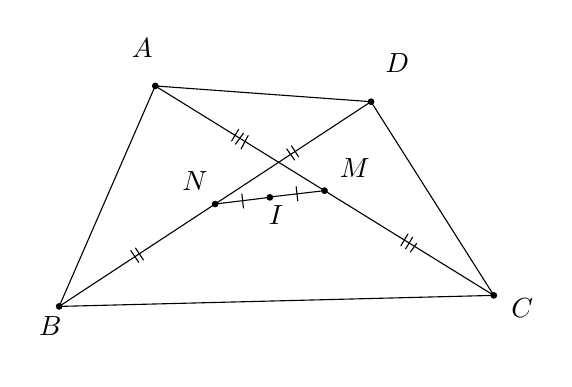
\begin{tikzpicture}[line cap=round,line join=round,>=stealth,x=1.0cm,y=1.0cm,scale=1]
				\clip(-0.44,-0.06) rectangle (6.12,4.14);
				\draw (1.18,3.4)-- (-0.04,0.6);
				\draw (-0.04,0.6)-- (5.48,0.74);
				\draw (5.48,0.74)-- (3.92,3.2);
				\draw (3.92,3.2)-- (1.18,3.4);
				\draw (0.76,4.12) node[anchor=north west] {$A$};
				\draw (-0.42,0.6) node[anchor=north west] {$B$};
				\draw (5.58,0.82) node[anchor=north west] {$C$};
				\draw (3.98,3.94) node[anchor=north west] {$D$};
				\draw (3.4,2.6) node[anchor=north west] {$M$};
				\draw (1.4,2.44) node[anchor=north west] {$N$};
				\draw (2.5,2.) node[anchor=north west] {$I$};
				\draw (2.635,1.985)-- (1.94,1.9);
				\draw (2.3,1.85) -- (2.28,2.03);
				\draw (2.64,1.99)-- (3.33,2.07);
				\draw (2.97,2.12) -- (2.99,1.94);
				\draw (-0.04,0.6)-- (1.94,1.9);
				\draw (0.87,1.31) -- (0.97,1.16);
				\draw (0.93,1.34) -- (1.03,1.19);
				\draw (1.94,1.9)-- (3.92,3.2);
				\draw (2.85,2.6) -- (2.95,2.46);
				\draw (2.91,2.64) -- (3,2.5);
				\draw (1.18,3.4)-- (3.33,2.07);
				\draw (2.24,2.85) -- (2.15,2.7);
				\draw (2.3,2.8) -- (2.2,2.66);
				\draw (2.36,2.77) -- (2.27,2.6);
				\draw (3.33,2.07)-- (5.48,0.74);
				\draw (4.39,1.52) -- (4.3,1.37);
				\draw (4.45,1.48) -- (4.36,1.33);
				\draw (4.5,1.4) -- (4.42,1.29);
				\draw [fill=black] (1.18,3.4) circle (1pt);
				\draw [fill=black] (-0.04,0.6) circle (1pt);
				\draw [fill=black] (5.48,0.74) circle (1pt);
				\draw [fill=black] (3.92,3.2) circle (1pt);
				\draw [fill=black] (3.33,2.07) circle (1pt);
				\draw [fill=black] (1.94,1.9) circle (1pt);
				\draw [fill=black] (2.635,1.985) circle (1pt);
			\end{tikzpicture}
		}
		\noindent Mặt khác $I$ là trung điểm của $MN$ nên $ \overrightarrow {IM}  +  \overrightarrow{IN}= \overrightarrow {0}$.\\
		Vậy $ \overrightarrow {IA}  +  \overrightarrow{IB}  +  \overrightarrow{IC}  +  \overrightarrow{ID}=2 \overrightarrow {0}= \overrightarrow {0}$. \\
		b) Với điểm $O$ bất kì ta có
		\begin{eqnarray*}
			&& \overrightarrow{OA}  +  \overrightarrow{OC}=2 \overrightarrow {OM}, \\
			&& \overrightarrow{OB}  +  \overrightarrow{OD}=2 \overrightarrow {ON}, \\
			&& \overrightarrow{OM}  +  \overrightarrow{ON}=2 \overrightarrow {OI}.
		\end{eqnarray*}
		Do đó
		\begin{eqnarray*}
			\overrightarrow {OA}  +  \overrightarrow{OB}  +  \overrightarrow{OC}  +  \overrightarrow{OD}  &=&  \left( \overrightarrow {OA}  +  \overrightarrow{OC}\right)  +  \left( \overrightarrow {OB}  +  \overrightarrow{OD}\right) \\
			&=&2 \overrightarrow {OM}  +  2 \overrightarrow {ON} \\
			&=&2\left( \overrightarrow {OM}  +  \overrightarrow{ON}\right) \\
			&=&4 \overrightarrow {OI}.
		\end{eqnarray*}
	}
\end{bt}


\begin{bt}%[Huỳnh Đức Vũ, BG10-2022, Nhóm 9]%[0H1G3]
	Cho tam giác $ABC$ không vuông. Gọi $G$, $H$, $O$ lần lượt là trọng tâm, trực tâm, tâm đường tròn ngoại tiếp tam giác $ABC$. Gọi $D$ là điểm đối xứng của $A$ qua $O$ và $M$ là trung điểm của cạnh $BC$. Chứng minh
	\begin{multicols}{2}
		\begin{enumerate}
			\item  $\overrightarrow{HB}+\overrightarrow{HC}=\overrightarrow{HD}$.
			\item  $\overrightarrow{HA}+\overrightarrow{HB}+\overrightarrow{HC}=2\overrightarrow{HO}$.
			\item   $\overrightarrow{HA}-\overrightarrow{HB}-\overrightarrow{HC}=2\overrightarrow{OA}$.
			\item  $\overrightarrow{OA}+\overrightarrow{OB}+\overrightarrow{OC}=\overrightarrow{OH}$.
			\item  $\overrightarrow{OH}=3\overrightarrow{OG}$.
			\item  $\overrightarrow{AH}=2\overrightarrow{OM}$.
		\end{enumerate}
	\end{multicols}
	\loigiai{
		\begin{enumerate}
			\item Chứng minh $\overrightarrow{HB}+\overrightarrow{HC}=\overrightarrow{HD}$.
			      \immini{
				      Ta có $BH\parallel CD$ (vì cùng vuông góc với $AC$).\\
				      Và $BD\parallel CH$ (vì cùng vuông góc với $AB$).\\
				      Suy ra $BDCH$ là hình bình hành.\\
				      Vậy $\overrightarrow{HB}+\overrightarrow{HC}=\overrightarrow{HD}$ (quy tắc hình bình hành).
			      }{
				      \begin{tikzpicture}[scale=1,font=\footnotesize,line join=round,line cap=round,>=stealth]
					      \path
					      (0,0) coordinate (O)
					      ($(O)+(120:3cm)$) coordinate (A)
					      ($(O)+(-30:3cm)$) coordinate (C)
					      ($(O)+(210:3cm)$) coordinate (B)
					      ($(B)!0.5!(C)$) coordinate (M)
					      ($(B)!0.5!(A)$) coordinate (N)
					      ($(A)!2/3!(M)$) coordinate (G)
					      ($2*(O)-(A)$) coordinate (D)
					      ($(B)!(A)!(C)$) coordinate (A1)
					      ($(A)!(B)!(C)$) coordinate (B1)
					      (intersection of A--A1 and B--B1) coordinate (H)
					      ;
					      \draw (O) circle(3cm) (A)--(B)--(C)--cycle (A)--(A1) (H)--(C)--(D)--(B)--(B1) (M)--(A)--(D) (M)--(O)--(H)--(D) (C)--(N);
					      \foreach \p/\q in {O/10,A/90,C/-20,B/-190,G/60,H/140,M/-90,D/-45}
					      \fill[black] (\p) circle (1.0pt) ($(\p)+(\q:2.5mm)$) node{$\p$};
					      \tkzMarkRightAngles(A,A1,C B,B1,C A,B,D A,C,D O,M,C)
				      \end{tikzpicture}
			      }
			\item Chứng minh
			      $\overrightarrow{HA}+\overrightarrow{HB}+\overrightarrow{HC}=2\overrightarrow{HO}$.\\
			      Ta có
			      \allowdisplaybreaks
			      \begin{eqnarray*}
				      \overrightarrow{HA}+\overrightarrow{HB}+\overrightarrow{HC}
				      &=&\overrightarrow{HA}+\overrightarrow{HD}\text{ (theo ý trên)}\\
				      &=&2\overrightarrow{HO} \text{ (vì } O \text{ là trung điểm của } AD).
			      \end{eqnarray*}
			\item Chứng minh  $\overrightarrow{HA}-\overrightarrow{HB}-\overrightarrow{HC}=2\overrightarrow{OA}$.\\
			      Ta có
			      $$\overrightarrow{HA}-\overrightarrow{HB}-\overrightarrow{HC}=\overrightarrow{HA}-\left(\overrightarrow{HB}+\overrightarrow{HC}\right)=\overrightarrow{HA}-\overrightarrow{HD}=\overrightarrow{DA}=2\overrightarrow{OA}.$$
			\item Chứng minh  $\overrightarrow{OA}+\overrightarrow{OB}+\overrightarrow{OC}=\overrightarrow{OH}$.\\
			      Ta có
			      \begin{eqnarray*}
				      \overrightarrow{OA}+\overrightarrow{OB}+\overrightarrow{OC} &=&3\overrightarrow{OH}+\overrightarrow{HA}+\overrightarrow{HB}+\overrightarrow{HC} \text{ (Quy tắc 3 điểm)}\\
				      &=&3\overrightarrow{OH}+2\overrightarrow{HO}\text{ (theo ý (2))}\\
				      &=&\overrightarrow{OH}.
			      \end{eqnarray*}
			\item Chứng minh $\overrightarrow{OH}=3\overrightarrow{OG}$.\\
			      Theo ý $(4)$ ta có $\overrightarrow{OA}+\overrightarrow{OB}+\overrightarrow{OC}=\overrightarrow{OH}$.\\
			      Mặt khác, $G$ là trọng tâm tam giác $ABC$ nên $\overrightarrow{OA}+\overrightarrow{OB}+\overrightarrow{OC}=3\overrightarrow{OG}$.\\
			      Suy ra $\overrightarrow{OH}=3\overrightarrow{OG}$.
			\item Chứng minh $\overrightarrow{AH}=2\overrightarrow{OM}$.\\
			      Trong tam giác $AHD$, ta có $OM$ là đường trung bình nên $\overrightarrow{AH}=2\overrightarrow{OM}$.
		\end{enumerate}}
\end{bt}

\begin{bt}%[Huỳnh Đức Vũ, BG10-2022, Nhóm 9]%[0H1B3-2]
	Cho tam giác $ABC$. Gọi $M$ là điểm trên cạnh $BC$ sao cho $MB=2MC$. Biết rằng  $\overrightarrow {AB}  +  2 \overrightarrow {AC}=x\overrightarrow{AM}$. Tìm $x$.\\
	
	\loigiai{
		\begin{center}
			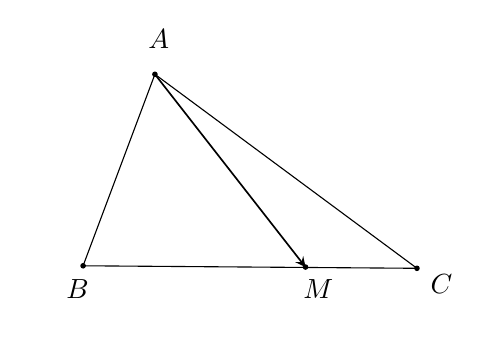
\begin{tikzpicture}[line cap=round,line join=round,>=stealth,x=1.0cm,y=1.0cm,scale=0.8]
				\clip(-0.14,0.12) rectangle (6.66,4.7);
				\draw (1.88,3.96)-- (0.74,0.92);
				\draw (0.74,0.92)-- (6.04,0.88);
				\draw (6.04,0.88)-- (1.88,3.96);
				\draw [->,line width=0.6pt] (1.88,3.96) -- (4.27,0.9);
				\draw (1.62,4.82) node[anchor=north west] {$A$};
				\draw (6.1,0.94) node[anchor=north west] {$C$};
				\draw (4.08,0.86) node[anchor=north west] {$M$};
				\draw (0.32,0.86) node[anchor=north west] {$B$};
				\begin{scriptsize}
					\draw [fill=black] (1.88,3.96) circle (1pt);
					\draw [fill=black] (0.74,0.92) circle (1pt);
					\draw [fill=black] (6.04,0.88) circle (1pt);
					\draw [fill=black] (4.27,0.9) circle (1pt);
				\end{scriptsize}
			\end{tikzpicture}
		\end{center}
		\allowdisplaybreaks
		\begin{eqnarray*}
			M\;\text{là điểm thuộc cạnh}\;BC\;\text{và}\;MB=2MC &\Leftrightarrow& \overrightarrow{MB}=-2\overrightarrow{MC}\\
			&\Leftrightarrow& \overrightarrow{AB}-\overrightarrow{AM}=-2(\overrightarrow{AC}-\overrightarrow{AM})\\
			&\Leftrightarrow& \overrightarrow{AB}+2\overrightarrow{AC}=3\overrightarrow{AM}.
		\end{eqnarray*}
	}
\end{bt}
\begin{bt}%[Huỳnh Đức Vũ, BG10-2022, Nhóm 9]%[0H1K3-2]
	Cho tứ giác $ABCD$. Gọi $M,N$ lần lượt thuộc các đoạn thẳng $AB,CD$ sao cho $MB=2MA$ và $NC=2ND$. Biết rằng
	$2\overrightarrow {AD}+ \overrightarrow {BC}=x\overrightarrow{MN}$. Tìm $x$. \\
	
	\loigiai {
		Vì $M$, $N$ lần lượt thuộc các đoạn thẳng $AB$, $CD$ sao cho $MB=2MA$ và $NC=2ND$ nên ta có
		$2 \overrightarrow {MA}  +  \overrightarrow{MB}= \overrightarrow {0}$  và $2 \overrightarrow {DN}  +  \overrightarrow{CN}= \overrightarrow {0}$.
		\immini{
			Áp dụng quy tắc ba điểm, ta có
			\allowdisplaybreaks
			\begin{eqnarray*}
				&& \overrightarrow{MN}= \overrightarrow {MA}  +  \overrightarrow{AD}  +  \overrightarrow{DN}.\qquad(1) \\
				&& \overrightarrow{MN}= \overrightarrow {MB}  +  \overrightarrow{BC}  +  \overrightarrow{CN}\\&\Rightarrow& 2\overrightarrow{MN}= 2\overrightarrow {MB}  +  2\overrightarrow{BC}  +  2\overrightarrow{CN}.\qquad (2)
			\end{eqnarray*}
			Cộng $(1)$ và $(2)$ vế theo vế ta được
			\allowdisplaybreaks
			\begin{eqnarray*}
				&&3 \overrightarrow {MN}=\left(2 \overrightarrow {MA}  +  \overrightarrow{MB}\right)  +  2 \overrightarrow {AD}  +  \overrightarrow{BC}  +  \left(2 \overrightarrow {DN}  +  \overrightarrow{CN}\right)\\
				&\Leftrightarrow&3 \overrightarrow {MN}=2 \overrightarrow {AD}  +  \overrightarrow{BC}\\
				&\Leftrightarrow& \overrightarrow{MN}=\dfrac{2}{3} \overrightarrow {AD}  +  \dfrac{1}{3} \overrightarrow {BC}.
			\end{eqnarray*}}
		{
			\begin{tikzpicture}[line cap=round,line join=round,>=stealth,x=1.0cm,y=1.0cm,scale=0.8]
				\clip(-1.34,-1.02) rectangle (5.24,3.18);
				\draw (0.58,2.4)-- (-0.8,-0.18);
				\draw (-0.8,-0.18)-- (4.58,-0.18);
				\draw (4.58,-0.18)-- (4.19,2.15);
				\draw (4.19,2.15)-- (0.58,2.4);
				\draw [->,line width=0.6pt] (1.78,2.32) -- (1,-0.18);
				\draw (0.06,3.06) node[anchor=north west] {$A$};
				\draw (4.44,-0.24) node[anchor=north west] {$C$};
				\draw (4.28,2.76) node[anchor=north west] {$B$};
				\draw (1.94,3.04) node[anchor=north west] {$M$};
				\draw (0.76,-0.24) node[anchor=north west] {$N$};
				\draw (-1.16,-0.2) node[anchor=north west] {$D$};
				\begin{scriptsize}
					\draw [fill=black] (0.58,2.4) circle (1pt);
					\draw [fill=black] (-0.8,-0.18) circle (1pt);
					\draw [fill=black] (1,-0.18) circle (1pt);
					\draw [fill=black] (1.78,2.32) circle (1pt);
					\draw [fill=black] (4.18,2.15) circle (1pt);
					\draw [fill=black] (4.58,-0.18) circle (1pt);
				\end{scriptsize}
			\end{tikzpicture}
		}
	}
\end{bt}
\begin{bt}%[Huỳnh Đức Vũ, BG10-2022, Nhóm 9]%[0H1G3-2]
	Cho tam giác đều $ABC$ tâm $O$. Lấy $M$ là một điểm bất kì trong tam giác. Gọi $D$, $E$, $F$ lần lượt là hình chiếu của $M$ trên $BC$, $CA$, $AB$. Biết rằng  $\overrightarrow {MD}  +  \overrightarrow{ME} +  \overrightarrow{MF}=x \overrightarrow {MO}$, tìm $x$.
	\\
	
	\loigiai{
		\immini{Qua điểm $M$ dựng
			\begin{itemize}
				\item đường thẳng song song với $BC$, cắt các cặp đường thẳng $AB$, $AC$ tại $V$, $Z$;
				\item đường thẳng song song với $AB$, cắt các cặp đường thẳng $AC$, $BC$ tại $T$, $X$;
				\item đường thẳng song song với $BC$, cắt các cặp đường thẳng $AB$, $AC$ tại $V$, $Z$.
			\end{itemize}}	{
			\begin{tikzpicture}[scale=1, font=\footnotesize, line join=round, line cap=round, >=stealth]
				\clip(0.4,-1.24) rectangle (7.96,5.18);
				\draw(6.03,1.16) -- (5.84,1.06) -- (5.95,0.87) -- (6.13,0.98) -- cycle;
				\draw(5.01,-0.27) -- (4.8,-0.27) -- (4.8,-0.48) -- (5.0,-0.48) -- cycle;
				\draw(2.87,1.65) -- (2.98,1.83) -- (2.80,1.94) -- (2.69,1.76) -- cycle;
				\draw (1.38,-0.42)-- (6.96,-0.52);
				\draw (4.26,4.36)-- (1.38,-0.42);
				\draw (4.26,4.36)-- (6.96,-0.52);
				\draw (3.5,3.10)-- (5.49,-0.49);
				\draw (1.88,0.42)-- (6.49,0.33);
				\draw (5.78,1.62)-- (4.52,-0.48);
				\draw (5.02,0.36)-- (5.0,-0.48);
				\draw (5.02,0.36)-- (6.13,0.98);
				\draw (5.02,0.36)-- (2.7,1.76);
				\draw (0.58,-0.2) node[anchor=north west] {$B$};
				\draw (7.2,-0.34) node[anchor=north west] {$C$};
				\draw (3.8,-0.44) node[anchor=north west] {$X$};
				\draw (4.68,-0.44) node[anchor=north west] {$D$};
				\draw (5.38,-0.44) node[anchor=north west] {$Y$};
				\draw (4.7,1.4) node[anchor=north west] {$M$};
				\draw (5.7,2.54) node[anchor=north west] {$T$};
				\draw (6.04,1.86) node[anchor=north west] {$E$};
				\draw (6.36,1.2) node[anchor=north west] {$Z$};
				\draw (4.,5.2) node[anchor=north west] {$A$};
				\draw (2.94,3.72) node[anchor=north west] {$U$};
				\draw (2.02,2.3) node[anchor=north west] {$F$};
				\draw (1.22,0.94) node[anchor=north west] {$V$};
				\path
				(4.26,4.36)coordinate (A)
				(1.38,-0.42) coordinate (B)
				(6.96,-0.52) coordinate (C)
				($(B)!0.5!(C)$) coordinate (X)
				($(A)!0.66!(X)$) coordinate (O) node[above, left]{$O$};
				\draw (5.02,0.36)--(O);
				\begin{scriptsize}
					\draw [fill=black] (1.38,-0.42) circle (1.0pt);
					\draw [fill=black] (O) circle (1.0pt)[fill=black];
					\draw [fill=black] (6.96,-0.52) circle (1.0pt);
					\draw [fill=black] (4.26,4.36) circle (1.0pt);
					\draw [fill=black] (5.02,0.36) circle (1.0pt);
					\draw [fill=black] (3.5,3.1) circle (1.0pt);
					\draw [fill=black] (5.78,1.62) circle (1.0pt);
					\draw [fill=black] (6.49,0.33) circle (1.0pt);
					\draw [fill=black] (5.49,-0.49) circle (1.0pt);
					\draw [fill=black] (4.52,-0.48) circle (1.0pt);
					\draw [fill=black] (1.88,0.42) circle (1.0pt);
					\draw [fill=black] (2.69,1.76) circle (1.0pt);
					\draw [fill=black] (5,-0.48) circle (1.0pt);
					\draw [fill=black] (6.13,0.98) circle (1.0pt);
				\end{scriptsize}
			\end{tikzpicture}}
		Ta thấy các tứ giác $MTAU$, $MVBX$, $MYCZ$ là các hình bình hành và các điểm $D$, $E$, $F$ tương ứng là trung điểm của $XY$, $ZT$, $UV$.\\
		Từ đó suy ra
		\begin{eqnarray*}
			\overrightarrow {M D}  +  \overrightarrow{ME}  +  \overrightarrow{MF}&=&  \dfrac{1}{2}\left( \overrightarrow {M X}  +  \overrightarrow{MY}\right)+  \dfrac{1}{2}\left( \overrightarrow {M Z}  +  \overrightarrow{MT}\right) +  \dfrac{1}{2}\left( \overrightarrow {MU}  +  \overrightarrow{MV}\right) \\
			&=&\dfrac{1}{2}\left( \overrightarrow {MT}  +  \overrightarrow{MU}\right)  +  \dfrac{1}{2}\left( \overrightarrow {MV}  +  \overrightarrow{MX}\right)  +  \dfrac{1}{2}\left( \overrightarrow {MY}  +  \overrightarrow{M Z}\right) \\
			&=&\dfrac{1}{2}\left( \overrightarrow {MA}  +  \overrightarrow{MB}  +  \overrightarrow{MC}\right) \\
			&=&\dfrac{3}{2} \overrightarrow {MO}.
		\end{eqnarray*}
	}
\end{bt}
\begin{bt}%[Huỳnh Đức Vũ, BG10-2022, Nhóm 9]%[0H1B3-2]
	Cho hình bình hành $ABCD$ có tâm $O$ và $E$ là trung điểm $AD$. Tìm các số thực $x$ và $y$ biết rằng
	\begin{enumerate}
		\item  $\overrightarrow{EA} + \overrightarrow{EB} + 2\overrightarrow{EC} = x\overrightarrow{AB}$.
		\item  $\overrightarrow{EB} + 2\overrightarrow{EA} + 4\overrightarrow{ED} = y\overrightarrow{EC}$.
	\end{enumerate}

	\loigiai{
		\begin{center}
			\begin{tikzpicture}[line join = round, line cap = round,>=stealth,font=\footnotesize,scale=1]
				\tkzDefPoints{0/0/D}
				\coordinate (C) at ($(D)+(5,0)$);
				\tkzDefShiftPoint[D](70:3){A}
				\coordinate (B) at ($(A)+(C)-(D)$);
				\pgfresetboundingbox
				\draw (A)--(B) (A)--(C) (B)--(C) (D)--(C) (A)--(D) (B)--(D);
				\coordinate (O) at ($(A)!0.5!(C)$);
				\coordinate (E) at ($(A)!0.5!(D)$);
				\tkzDrawPoints[fill=black](A,B,C,D,O,E)
				\tkzLabelPoints[above](A,B)
				\tkzLabelPoints[left](E)
				\tkzLabelPoints[below](C,D,O)
			\end{tikzpicture}
		\end{center}
		\begin{enumerate}
			\item Theo tính chất trung điểm ta có $4\overrightarrow{EO} = 2\overrightarrow{AB}$.\\
			      Khi đó
			      {\allowdisplaybreaks
			      \begin{eqnarray*}
				      \overrightarrow{EA} + \overrightarrow{EB} + 2\overrightarrow{EC}&=&\overrightarrow{EA} + \overrightarrow{EB} + 2\overrightarrow{EC} \\
				      &=& \overrightarrow{EA} + \overrightarrow{EA} + \overrightarrow{AB} + 2\overrightarrow{EC}\\
				      &=& 2\left(\overrightarrow{EA} + \overrightarrow{EC}\right) + \overrightarrow{AB} \\
				      &=& 4\overrightarrow{EO} + \overrightarrow{AB} \\
				      &=& 2\overrightarrow{AB} + \overrightarrow{AB} = 3\overrightarrow{AB}.
			      \end{eqnarray*}}
			\item Ta có
			      {\allowdisplaybreaks
			      \begin{eqnarray*}
				      \overrightarrow{EB} + 2\overrightarrow{EA} + 4\overrightarrow{ED}&=&\overrightarrow{EB} + 2\overrightarrow{EA} + 4\overrightarrow{ED} \\
				      &=& \overrightarrow{EA} + \overrightarrow{AB} + 2\overrightarrow{ED} + 2\left(\overrightarrow{EA} + \overrightarrow{ED}\right)\\
				      &=& \left(\overrightarrow{EA} + \overrightarrow{ED}\right) + \overrightarrow{ED} + \overrightarrow{AB} \\
				      &=& \overrightarrow{ED} + \overrightarrow{DC} = \overrightarrow{EC}.
			      \end{eqnarray*}}
		\end{enumerate}
	}
\end{bt}
\begin{bt}%[Huỳnh Đức Vũ, BG10-2022, Nhóm 9]%[0H1B3-2]
	Cho tam giác $ABC$. Dựng bên ngoài tam giác các hình bình hành $ABIF$, $BCPQ$, $CARS$. Biết rằng $\overrightarrow{RF}+\overrightarrow{IQ}+\overrightarrow{PS}=x(\overrightarrow{AB}+\overrightarrow{AC})$. Tìm $x$.
	\\
	
	\loigiai{
		\immini{
			Ta có $\heva{& \overrightarrow{RF}=\overrightarrow{RA}+\overrightarrow{AF}&\quad(1) \\& \overrightarrow{IQ}=\overrightarrow{IB}+\overrightarrow{BQ} &\quad(2)\\& \overrightarrow{PS}=\overrightarrow{PC}+\overrightarrow{CS}.&\quad(3)}$\\
			Cộng vế theo vế của $(1)$, $(2)$, $(3)$, ta được\\  $\overrightarrow{RF}+\overrightarrow{IQ}+\overrightarrow{PS}=\underbrace{(\overrightarrow{RA}+\overrightarrow{CS})}_{\overrightarrow{0}}+\underbrace{(\overrightarrow{AF}+\overrightarrow{IB})}_{\overrightarrow{0}}+\underbrace{(\overrightarrow{BQ}+\overrightarrow{PC})}_{\overrightarrow{0}}$. \\
			Suy ra $\overrightarrow{RF}+\overrightarrow{IQ}+\overrightarrow{PS}=\overrightarrow{0}$.
		}{
			\begin{tikzpicture}[scale=1,font=\footnotesize,line join=round,line cap=round,>=stealth]
				\path
				(1,2.7) coordinate (A)
				(0,0) coordinate (B)
				(3.5,0) coordinate (C)
				(2,3.4) coordinate (R)
				($(R)+(C)-(A)$) coordinate (S)
				(-0.3,3.4) coordinate (F)
				($(F)+(B)-(A)$) coordinate (I)
				(0.6,-1) coordinate (Q)
				($(Q)+(C)-(B)$) coordinate (P)
				;
				\draw (A)--(B)--(C)--cycle (A)--(R)--(S)--(C) (A)--(F)--(I)--(B)
				(B)--(Q)--(P)--(C);
				\draw[->] (R)--(F);		\draw[->] (I)--(Q);    \draw[->] (P)--(S);
				\foreach \p/\q in {A/90,B/110,C/0,R/90,F/90,P/-90,Q/-90,I/180,S/0}
				\fill[black] (\p) circle (1.0pt) ($(\p)+(\q:2.5mm)$) node{$\p$};
			\end{tikzpicture}
		}
	}
\end{bt}

\begin{bt}%%[Huỳnh Đức Vũ, BG10-2022, Nhóm 9]%[0H1K3-2]
	Dựng bên ngoài tứ giác $ABCD$ các hình bình hành $ABEF$, $BCGH$, $CDIJ$, $DAKL$.
	\begin{enumerate}
		\item Chứng minh rằng  $\overrightarrow{KF}+\overrightarrow{EH}+\overrightarrow{GJ}+\overrightarrow{IL}=\overrightarrow{0}$.
		\item Chứng minh rằng  $\overrightarrow{EL}-\overrightarrow{HI}=\overrightarrow{FK}-\overrightarrow{GJ}$.
	\end{enumerate}
	\loigiai{
		\begin{enumerate}
			\item Chứng minh rằng  $\overrightarrow{KF}+\overrightarrow{EH}+\overrightarrow{GJ}+\overrightarrow{IL}=\overrightarrow{0}$.
			      \immini{Ta có
				      \allowdisplaybreaks
				      \begin{eqnarray*}
					      && \overrightarrow{KF}=\overrightarrow{KA}+\overrightarrow{AF}.\quad(1)\\
					      &&	\overrightarrow{EH}=\overrightarrow{EB}+\overrightarrow{BH}. \quad(2)\\
					      && \overrightarrow{GJ}=\overrightarrow{GC}+\overrightarrow{CJ}. \quad(3)\\
					      && \overrightarrow{IL}=\overrightarrow{ID}+\overrightarrow{DL}.\quad(4)
				      \end{eqnarray*}
				      Cộng vế theo vế của $(1)$, $(2)$, $(3)$, $(4)$ ta được
				      \allowdisplaybreaks
				      \begin{eqnarray*}
					      &&\overrightarrow{KF}+\overrightarrow{EH}+\overrightarrow{GJ}+\overrightarrow{IL}\\
					      &=&\underbrace{(\overrightarrow{KA}+\overrightarrow{DL})}_{\overrightarrow{0}}+\underbrace{(\overrightarrow{EB}+\overrightarrow{AF})}_{\overrightarrow{0}}+\underbrace{(\overrightarrow{BH}+\overrightarrow{GC})}_{\overrightarrow{0}}+\underbrace{(\overrightarrow{CJ}+\overrightarrow{ID})}_{\overrightarrow{0}}.
				      \end{eqnarray*}
				      Suy ra $\overrightarrow{KF}+\overrightarrow{EH}+\overrightarrow{GJ}+\overrightarrow{IL}=\overrightarrow{0}$ (đpcm).
			      }{
				      \begin{tikzpicture}[scale=0.9,font=\footnotesize,line join=round,line cap=round,>=stealth]
					      \path
					      (1,3) coordinate (A)
					      (0,0) coordinate (B)
					      (3.5,0) coordinate (C)
					      (3,2) coordinate (D)
					      (-0.3,3.2) coordinate (F)
					      ($(F)+(B)-(A)$) coordinate (E)
					      (0.4,-1.2) coordinate (H)
					      ($(H)+(C)-(B)$) coordinate (G)
					      (4,0.5) coordinate (J)
					      ($(J)+(D)-(C)$) coordinate (I)
					      (3.6,3.4) coordinate (L)
					      ($(L)+(A)-(D)$) coordinate (K)
					      ;
					      \draw (A)--(B)--(C)--(D)--cycle (A)--(F)--(E)--(B) (B)--(H)--(G)--(C) (C)--(J)--(I)--(D)--(L)--(K)--(A);
					      \draw[->] (K)--(F);
					      \draw[->] (E)--(H); \draw[->] (G)--(J); \draw[->] (I)--(L);
					      \foreach \p/\q in {A/120,B/-140,C/0,D/-150,E/180,F/170,G/-90,H/-90,I/0,J/0, K/90,L/0}
					      \fill[black] (\p) circle (1.0pt) ($(\p)+(\q:3mm)$) node{$\p$};
				      \end{tikzpicture}
			      }
			\item Chứng minh rằng  $\overrightarrow{EL}-\overrightarrow{HI}=\overrightarrow{FK}-\overrightarrow{GJ}$.\\
			      Ta có
			      \begin{eqnarray*}
				      \overrightarrow{EL}-\overrightarrow{HI}
				      &=&\overrightarrow{EB}+\overrightarrow{BC}+\overrightarrow{CD}+\overrightarrow{DL} -\left(\overrightarrow{HG}+\overrightarrow{GC}+\overrightarrow{CD}+\overrightarrow{DI}\right)\\
				      &=&\overrightarrow{EB}+\overrightarrow{DL}-\left(\overrightarrow{GC}+\overrightarrow{DI}\right) \left(\text{vì } BCGH \text{ là hình bình hành nên }\overrightarrow{BC}=\overrightarrow{HG}\right)\\
				      &=&\overrightarrow{FA}+\overrightarrow{AK}-\left(\overrightarrow{GC}+\overrightarrow{CJ}\right)\\
				      &=&\overrightarrow{FK}-\overrightarrow{GJ}.
			      \end{eqnarray*}
		\end{enumerate}
		(Vì $ABEF$, $ADLK$, $CDIJ$ là các hình bình hành nên $\overrightarrow{EB}=\overrightarrow{FA}$,  $\overrightarrow{DL}=\overrightarrow{AK}$,  $\overrightarrow{DI}=\overrightarrow{CJ}$.)}
\end{bt}
\begin{bt}%[Huỳnh Đức Vũ, BG10-2022, Nhóm 9]%[0H1G3-2]
	Cho đường tròn $(I)$ nội tiếp tam giác $ABC$ có $AB=c$, $AC=b$, $BC=a$. Chứng minh rằng
	$$a \overrightarrow {IA}  +  b \overrightarrow {IB}  +  c \overrightarrow {IC}= \overrightarrow {0}.$$
	\loigiai{
		\immini{
			Qua $C$ dựng đường thẳng song song với $IA$, cắt đường thẳng $BI$ tại $E$.\\
			Qua $C$ dựng đường thẳng song song với $IB$, cắt đường thẳng $AI$ tại $F$.\\
			$IECF$ là hình bình hành nên $ \overrightarrow {IC}= \overrightarrow {IE}  +  \overrightarrow{IF}.\qquad(1)$.\\
			Gọi $D$ là giao điểm của $AI$ và $BC$.
			Vì $ID\parallel CE$ và $AD$ là đường phân giác nên ta có  $$\dfrac{BI}{IE}=\dfrac{BD}{DC}=\dfrac{AB}{AC}=\dfrac{c}{b}
				\Rightarrow \overrightarrow{IE}= -  \dfrac{b}{c} \overrightarrow {IB}.\qquad(2)$$
			Tương tự ta chứng minh được $ \overrightarrow {IF}= -  \dfrac{a}{c} \overrightarrow {IA}.\qquad(3)$ \\
			Từ $(1)$, $(2)$, $(3)$ suy ra
			$$ \overrightarrow {IC}= -  \dfrac{b}{c} \overrightarrow {IB}  -  \dfrac{a}{c} \overrightarrow {IA}\Leftrightarrow a \overrightarrow {IA}  +  b \overrightarrow {IB}  +  c \overrightarrow {IC}= \overrightarrow {0}.$$
		}
		{
			\begin{tikzpicture}[scale=0.7,font=\footnotesize,line join=round,line cap=round,>=stealth]
				\clip(-1.2,-2.34) rectangle (5.44,3.74);
				\draw (0.9,3.08)-- (-0.2,-0.14);
				\draw  (-0.2,-0.14)-- (4.57,-0.2);
				\draw  (0.9,3.08)-- (4.57,-0.2);
				\draw  (-0.2,-0.14)-- (3.81,2.7);
				\draw (0.9,3.08)-- (2.20,-1.87);
				\draw  (3.81,2.7)-- (4.57,-0.2);
				\draw  (2.2,-1.87)-- (4.57,-0.2);
				\draw  (4.57,-0.2)-- (1.44,1.02);
				\draw (0.7,3.84) node[anchor=north west] {$A$};
				\draw (4.84,0.2) node[anchor=north west] {$C$};
				\draw (0.88,1.54) node[anchor=north west] {$I$};
				\draw (4.02,3.22) node[anchor=north west] {$E$};
				\draw (2.38,-1.66) node[anchor=north west] {$F$};
				\draw (1.18,-0.12) node[anchor=north west] {$D$};
				\draw (-0.46,-0.22) node[anchor=north west] {$B$};
				\begin{scriptsize}
					\draw [fill=black] (0.9,3.08) circle (0.6pt);
					\draw [fill=black] (-0.2,-0.14) circle (1pt);
					\draw [fill=black] (4.57,-0.2) circle (1pt);
					\draw [fill=black] (1.44,1.02) circle (1pt);
					\draw [fill=black] (2.43,1.72) circle (1pt);
					\draw [fill=black] (1.75,-0.16) circle (1pt);
					\draw [fill=black] (3.81,2.7) circle (1pt);
					\draw [fill=black] (2.2,-1.87) circle (1pt);
				\end{scriptsize}
			\end{tikzpicture}
		}
		\noindent \textit{Bài tập tương tự:} Cho đường tròn $(I)$ nội tiếp tam giác $ABC$. Chứng minh rằng
		\[\sin A\cdot \overrightarrow {IA}  +  \sin B\cdot \overrightarrow {IB}  +  \sin C\cdot \overrightarrow {IC}= \overrightarrow {0}.\]
	}
\end{bt}

\begin{bt}%[Huỳnh Đức Vũ, BG10-2022, Nhóm 9]%[0H1G3-2]
	Cho tam giác $ABC$ và một điểm $M$ bất kì nằm trong tam giác $ABC$. Đặt $S_{MBC}=S_a$, $S_{MCA}=S_b$, $S_{MAB}=S_c$. Chứng minh rằng
	\[S_a \overrightarrow {MA}  +  S_b \overrightarrow {MB}  +  S_c \overrightarrow {MC}= \overrightarrow {0}.\]
	\loigiai{
		\immini{
			Gọi $A'$ là giao điểm của đường thẳng $MA$ với $BC$.\\
			Ta có  $ \overrightarrow {MA'}=\dfrac{A'C}{BC} \overrightarrow {MB}  +  \dfrac{A'B}{BC} \overrightarrow {MC}$.\\
			Mà $\dfrac{A'C}{A'B}=\dfrac{S_{MA'C}}{S_{MA'B}}=\dfrac{S_{MAC}}{S_{MAB}}=\dfrac{S_b}{S_c}$ nên
			$$\dfrac{A'C}{BC}=\dfrac{S_b}{S_b  +  S_c},\;
				\dfrac{A'B}{BC}=\dfrac{S_c}{S_c  +  S_b}.$$
			Suy ra $\overrightarrow{MA'}=\dfrac{S_b}{S_b  +  S_c} \overrightarrow {MB}  +  \dfrac{S_c}{S_b  +  S_c} \overrightarrow {MC}.\qquad(1)$}
		{
			\begin{tikzpicture}[line cap=round,line join=round,>=triangle 45,x=1.0cm,y=1.0cm]
				\clip(1.3,-0.04) rectangle (7.66,4.04);
				\draw (3.56,3.36)-- (1.98,0.82);
				\draw (1.98,0.82)-- (6.64,0.78);
				\draw (6.64,0.78)-- (3.56,3.36);
				\draw (3.56,3.36)-- (5.08,0.8);
				\draw (4.58,1.64)-- (1.98,0.82);
				\draw (4.58,1.64)-- (6.64,0.78);
				\draw (3.36,4.04) node[anchor=north west] {$A$};
				\draw (1.4,1.0) node[anchor=north west] {$B$};
				\draw (6.8,1.06) node[anchor=north west] {$C$};
				\draw (3.75,2.15) node[anchor=north west] {$M$};
				\draw (4.9,0.8) node[anchor=north west] {$A'$};
				\begin{scriptsize}
					\draw [fill=black] (3.56,3.36) circle (1.0pt);
					\draw [fill=black] (1.98,0.82) circle (1.0pt);
					\draw [fill=black] (6.64,0.78) circle (1.0pt);
					\draw [fill=black] (5.08,0.8) circle (1.0pt);
					\draw [fill=black] (4.58,1.64) circle (1.0pt);
				\end{scriptsize}
			\end{tikzpicture}
		}
		\noindent	Mặt khác
		$$\dfrac{MA'}{MA}=\dfrac{S_{MA'B}}{S_{MAB}}=\dfrac{S_{MA'C}}{S_{MAC}}=\dfrac{S_{MA'B}  +  S_{MA'C}}{S_{MAB}  +  S_{MAC}}=\dfrac{S_a}{S_b  +  S_c}
			\Rightarrow \overrightarrow{MA'}=\dfrac{ -  S_a}{S_b  +  S_c} \overrightarrow {MA}. \qquad(2)$$ \\ Thay $(2)$ vào $(1)$ ta được\\
		$$  -  S_a \overrightarrow {MA}=S_b \overrightarrow {MB}  +  S_c \overrightarrow {MC}\Leftrightarrow S_a \overrightarrow {MA}  +  S_b \overrightarrow {MB}  +  S_c \overrightarrow {MC}= \overrightarrow {0}.$$
	}
\end{bt}
\begin{note}
	\begin{enumerate}
		\item Cho $M$ trùng với trọng tâm $G$ của tam giác $ABC$, ta được $ \overrightarrow {GA}  +  \overrightarrow{GB}  +  \overrightarrow{GC}= \overrightarrow {0}$.
		\item Cho $M$ trùng với tâm đường tròn nội tiếp $I$ của tam giác $ABC$, ta được kết quả\\ \[a\overrightarrow {IA}  +  b\overrightarrow {IB}  +  c\overrightarrow {IC}= \overrightarrow {0}.\]
		\item Nếu tam giác $ABC$ đều thì với điểm $M$ bất kì trong tam giác, Ta có
		      \[x\overrightarrow {MA}  +  y\overrightarrow {MB}  +  z\overrightarrow {MC}= \overrightarrow {0},\]
		      trong đó $x,y,z$ lần lượt là khoảng cách từ $M$ đến các cạnh $BC,CA$ và $AB$.
		\item Khi $M$ nằm ngoài tam giác $ABC$, ta có các kết quả như sau
		      \begin{enumerate}
			      \item Nếu $M$ thuộc góc $\widehat{BAC}$ và góc đối đỉnh của nó thì  $$  -  S_a\overrightarrow {MA}  +  S_b\overrightarrow {MB}  +  S_c\overrightarrow {MC}= \overrightarrow {0}.$$
			      \item Nếu $M$ thuộc góc $\widehat{ABC}$ và góc đối đỉnh của nó thì  $$S_a\overrightarrow {MA}  -  S_b\overrightarrow {MB}  +  S_c\overrightarrow {MC}= \overrightarrow {0}.$$
			      \item Nếu $M$ thuộc góc $\widehat{ACB}$ và góc đối đỉnh của nó thì  $$S_a\overrightarrow {MA}  +  S_b\overrightarrow {MB}  -S_c\overrightarrow {MC}= \overrightarrow {0}.$$
		      \end{enumerate}
	\end{enumerate}
\end{note}
% \setcounter{ex}{0}
\subsubsection{Bài tập trắc nghiệm}
\Opensolutionfile{ansbook}[ans/ansbook-0H1-3-2]
\Opensolutionfile{ans}[ans/ans-0H1-3-2]
\begin{ex}%[Huỳnh Đức Vũ-BG10-2022]%[0H1Y3-2]
	Cho tam giác $ABC$ có trọng tâm $G$. Gọi $M$ là trung điểm $AB$. Chọn mệnh đề \textbf{sai} trong các mệnh đề sau:
	\choice
	{$\overrightarrow{CM}=-3\overrightarrow{MG}$}
	{\True $\overrightarrow{GA}+\overrightarrow{GB}+\overrightarrow{GC}=\overrightarrow{AC}$}
	{$\overrightarrow{AB}+\overrightarrow{AC}=3\overrightarrow{AG}$}
	{$\overrightarrow{OA}+\overrightarrow{OB}+\overrightarrow{OC}=3\overrightarrow{OG}$, $O$ là điểm bất kì}
	\loigiai{
		\immini{
			Vì $G$ là trọng tâm tam giác $ABC$ nên ta có $$\overrightarrow{GA}+\overrightarrow{GB}+\overrightarrow{GC}=\overrightarrow{0}.$$
		} {
			\begin{tikzpicture}[scale=1, font=\footnotesize,line join=round, line cap=round, >=stealth]
				\path (0,0)coordinate(B)--(4,0)coordinate(A)--(1.5,2)coordinate(C);
				\coordinate (M) at ($(B)!0.5!(A)$);
				\coordinate (G) at ($(C)!2/3!(M)$);
				\draw (A)--(B)--(C)--cycle (A)--(M)--(C) (B)--(G)--(A);
				\foreach \x/\g in {C/90,B/-90,A/-90,M/-90,G/45} \fill (\x) circle (1pt)+(\g:0.25)node{$\x$};
			\end{tikzpicture}}}
\end{ex}
\begin{ex}%[Huỳnh Đức Vũ, BG10-2022, Nhóm 9]%[0H1Y3-2]
	Cho hình bình hành $ABCD$ tâm $O$. Khẳng định nào sau đây là \textbf{đúng}?
	\choice
	{$\overrightarrow{AB} + \overrightarrow{AD} = 2 \overrightarrow{AC}$}
	{\True $\overrightarrow{AB} + \overrightarrow{AD} = 2\overrightarrow{AO}$}
	{$\overrightarrow{AB} + \overrightarrow{AD} = \overrightarrow{CA}$}
	{$\overrightarrow{AB} + \overrightarrow{AD}=\overrightarrow{BD}$}
	\loigiai{\immini{
			Theo quy tắc hình bình hành ta có $\overrightarrow{AB} + \overrightarrow{AD} = \overrightarrow{AC}$.\\
			Mặt khác $O$ là trung điểm $AC$ nên $\overrightarrow{AC} = 2 \overrightarrow{AO}$.\\
			Vậy $\overrightarrow{AB} + \overrightarrow{AD} = 2 \overrightarrow{AO}$.}
		{\begin{tikzpicture}[>=stealth,line join=round,line cap=round,font=\footnotesize,scale=0.8]
				\tkzDefPoints{0/0/A,4/0/D,1/2.5/B}
				\coordinate (C) at ($(B)+(D)-(A)$);
				\coordinate (O) at ($(A)!.5!(C)$);
				% \tkzDrawVectors(A,B A,D A,C A,O)
				\tkzDrawSegments(A,C C,B C,D B,D A,B A,D)
				\tkzDrawPoints[fill=black](A,B,C,D,O)
				\tkzLabelPoints[above](O)
				\tkzLabelPoints[left](A,B)
				\tkzLabelPoints[right](D,C)
			\end{tikzpicture}}
	}
\end{ex}
\begin{ex}%[Huỳnh Đức Vũ, BG10-2022, Nhóm 9]%[0H1Y3-2]
	Cho $I$ là trung điểm của đoạn thẳng $AB$. Với điểm $M$ bất kỳ, ta luôn có
	\choice
	{$\overrightarrow{MA}+\overrightarrow{MB}=\overrightarrow{MI}$}
	{\True $\overrightarrow{MA}+\overrightarrow{MB}=2\overrightarrow{MI}$}
	{$\overrightarrow{MA}+\overrightarrow{MB}=3\overrightarrow{MI}$}
	{$\overrightarrow{MA}+\overrightarrow{MB}=\dfrac{1}{2}\overrightarrow{MI}$}
	\loigiai{
		Áp dụng tính chất trung điểm của đoạn thẳng: Với điểm $M$ bất kỳ, ta luôn có $\overrightarrow{MA}+\overrightarrow{MB}=2\overrightarrow{MI}$.}
\end{ex}
\begin{ex}%[Huỳnh Đức Vũ, BG10-2022, Nhóm 9]%[0H1Y3-2]
	Cho $G$ là trọng tâm của tam giác $ABC$. Với mọi điểm $M$, ta luôn có:
	\choice
	{$\overrightarrow{MA}+\overrightarrow{MB}+\overrightarrow{MC}=\overrightarrow{MG}$}
	{$\overrightarrow{MA}+\overrightarrow{MB}+\overrightarrow{MC}=2\overrightarrow{MG}$}
	{\True $\overrightarrow{MA}+\overrightarrow{MB}+\overrightarrow{MC}=3\overrightarrow{MG}$}
	{$\overrightarrow{MA}+\overrightarrow{MB}+\overrightarrow{MC}=4\overrightarrow{MG}$}
	\loigiai{
		Áp dụng tính chất trọng tâm của tam giác: Với mọi điểm $M$, ta luôn có $\overrightarrow{MA}+\overrightarrow{MB}+\overrightarrow{MC}=3\overrightarrow{MG}$.}
\end{ex}
\begin{ex}%[Huỳnh Đức Vũ, BG10-2022, Nhóm 9]%[0H1Y3-2]
	Cho $\triangle ABC$ có $G$ là trọng tâm, $I$ là trung điểm $BC$. Đẳng thức nào đúng?
	\choice
	{$\overrightarrow{GA}=2\overrightarrow{GI}$}
	{$\overrightarrow{IG}=-\dfrac{1}{3}\overrightarrow{IA}$}
	{\True $\overrightarrow{GB}+\overrightarrow{GC}=2\overrightarrow{GI}$}
	{$\overrightarrow{GB}+\overrightarrow{GC}=\overrightarrow{GA}$}
	\loigiai{
		\begin{center}
			\begin{tikzpicture}[scale=1, font=\footnotesize,line join=round, line cap=round, >=stealth]
				\path (0,0)coordinate(B)--(4,0)coordinate(C)--(1.5,2)coordinate(A);
				\coordinate (I) at ($(B)!0.5!(C)$);
				\coordinate (G) at ($(A)!2/3!(I)$);
				\draw (A)--(B)--(C)--cycle (A)--(I) (B)--(G)--(C);
				\foreach \x/\g in {A/90,B/-90,C/-90,I/-90,G/45} \fill (\x) circle (1pt)+(\g:0.25)node{$\x$};
			\end{tikzpicture}
		\end{center}
		Áp dụng tính chất trung điểm của đoạn thẳng, ta có $\overrightarrow{GB}+\overrightarrow{GC}=2\overrightarrow{GI}$.}
\end{ex}
\begin{ex}%[Huỳnh Đức Vũ, BG10-2022, Nhóm 9]%[0H1B3-2]
	Khẳng định nào sau đây \textbf{không phải} là điều kiện cần và đủ để $G$ là trọng tâm $\Delta ABC$, với $M$ là trung điểm của $BC$ và $O$ là điểm bất kì?
	\choice
	{$\overrightarrow{AG}=\dfrac{1}{3} \left( \overrightarrow{AB}+\overrightarrow{AC} \right)$}
	{\True $ \overrightarrow{OA}+\overrightarrow{OB}+\overrightarrow{OC}+3\overrightarrow{OG}=\overrightarrow{0}$}
	{$\overrightarrow{AG}+\overrightarrow{BG}+\overrightarrow{CG}=\overrightarrow{0}$}
	{$\overrightarrow{GM}=-\dfrac{1}{2} \overrightarrow{GA}$}
	\loigiai{
		Xét khẳng định $ \overrightarrow{OA}+\overrightarrow{OB}+\overrightarrow{OC}+3\overrightarrow{OG}=\overrightarrow{0}$, ta có \\
		$ \overrightarrow{OA}+\overrightarrow{OB}+\overrightarrow{OC}+3\overrightarrow{OG}=\overrightarrow{0} \Leftrightarrow 6 \overrightarrow{OG}=\overrightarrow{0} \Leftrightarrow G \equiv O$ với mọi điểm $O$ (vô lí).\\
		Vậy khẳng định $ \overrightarrow{OA}+\overrightarrow{OB}+\overrightarrow{OC}+3\overrightarrow{OG}=\overrightarrow{0}$ không phải là điều kiện cần và đủ để $G$ là trọng tâm $\Delta ABC$.
	}
\end{ex}
\begin{ex}%[Huỳnh Đức Vũ, BG10-2022, Nhóm 9]%[0H1B3-2]
	Cho $I$ là trung điểm của đoạn thẳng $AB$. Với $M$ là một điểm bất kỳ, tìm đẳng thức \textbf{đúng}.
	\choice
	{\True $\overrightarrow{MA}+\overrightarrow{MB}=2\overrightarrow{MI}$}
	{$\overrightarrow{MA}+\overrightarrow{MB}=\dfrac{1}{2}\overrightarrow{MI}$}
	{$\overrightarrow{MA}+\overrightarrow{MB}=\overrightarrow{MI}$}
	{$\overrightarrow{MA}+\overrightarrow{MB}=2\overrightarrow{IM}$}
	\loigiai{Áp dụng tính chất trung điểm.}\end{ex}
\begin{ex}%[Huỳnh Đức Vũ, BG10-2022, Nhóm 9]%[0H1B3-2]
	Cho tam giác $ABC$ có trọng tâm $G$ và $M$ là trung điểm của $AB$. Mệnh đề nào sau đây \textbf{sai}?
	\choice
	{$\overrightarrow{GA} + \overrightarrow{GB} + \overrightarrow{GC} = \overrightarrow{0}$}
	{$\overrightarrow{GA} + \overrightarrow{GB} = 2\overrightarrow{GM}$}
	{\True $\overrightarrow{MA} + \overrightarrow{MB} + \overrightarrow{MC} = \overrightarrow{0}$}
	{$\overrightarrow{MA} + \overrightarrow{MB} + \overrightarrow{MC} = 3\overrightarrow{MG}$}
	\loigiai
	{\immini
		{\begin{itemize}
				\item Vì $G$ là trọng tâm của tam giác $ABC$ nên $\overrightarrow{GA} + \overrightarrow{GB} + \overrightarrow{GC} = \overrightarrow{0}$.
				\item Vì $M$ là trung điểm của $AB$ nên $\overrightarrow{GA} + \overrightarrow{GB} = 2\overrightarrow{GM}$. ($G$ có thể tùy ý)
				\item Vì $G$ là trọng tâm của tam giác $ABC$ nên $\overrightarrow{MA} + \overrightarrow{MB} + \overrightarrow{MC} = 3\overrightarrow{MG}$. ($M$ có thể tùy ý)
				\item $\overrightarrow{MA} + \overrightarrow{MB} + \overrightarrow{MC} = \overrightarrow{0}$ là mệnh đề \textbf{sai}.
			\end{itemize}}
		{\begin{tikzpicture}[>=stealth,line join=round,line cap=round,font=\footnotesize,scale=0.7]
				\tkzDefPoints{0/0/A, 5/0/B, 2/3/C}
				\tkzDefMidPoint(A,B)\tkzGetPoint{M}
				\tkzCentroid(A,B,C)\tkzGetPoint{G}
				\tkzDrawPoints(A,B,C,M,G)
				\tkzDrawSegments(A,B B,C C,A C,M G,A G,B)
				\tkzMarkSegments[mark=|](M,A M,B)
				\tkzLabelPoints[above](C)
				%\tkzLabelPoints[left](B)
				%\tkzLabelPoints[right](C)
				\tkzLabelPoints[below](A,B,M)
				\node (G) at (2.6,1.3) {$G$};
			\end{tikzpicture}
		}
	}
\end{ex}
\begin{ex}%[Huỳnh Đức Vũ, BG10-2022, Nhóm 9]%[0H1B3-2]
	Cho $\triangle ABC$ có $M$, $Q$, $N$ lần lượt là trung điểm của $AB$, $BC$, $CA$. Khi đó vectơ \\ $\overrightarrow{AB}+\overrightarrow{BM}+\overrightarrow{NA}+\overrightarrow{BQ}$ là vectơ nào sau đây?
	\choice
	{\True $\overrightarrow{0}$}
	{$\overrightarrow{BC}$}
	{$\overrightarrow{AQ}$}
	{$\overrightarrow{CB}$}
	\loigiai{
		\immini{
			Ta có
			\allowdisplaybreaks
			\begin{eqnarray*}
				\overrightarrow{AB}+\overrightarrow{BM}+\overrightarrow{NA}+\overrightarrow{BQ}&=&\overrightarrow{NA}+\overrightarrow{AB}+\overrightarrow{BM}+\overrightarrow{BQ}\\
				&=&\overrightarrow{NM}+\overrightarrow{BQ}\\
				&=&\overrightarrow{0}.
			\end{eqnarray*}	}{\begin{tikzpicture}[>=stealth,line join=round,line cap=round,font=\footnotesize,scale=0.8]
				%\tkzInit[xmin=-1,ymin=-1,xmax=6,ymax=4]
				%\tkzClip
				\tkzDefPoints{0/0/A, -2/-2/B, 3/-2/C}
				\tkzDefMidPoint(A,B) \tkzGetPoint{M}
				\tkzDefMidPoint(A,C) \tkzGetPoint{N}
				\tkzDefMidPoint(C,B) \tkzGetPoint{Q}
				\tkzDrawPoints(A,B,C,M,N,Q)
				\tkzDrawSegments(A,B B,C C,A M,N N,Q)
				\tkzLabelPoints[above](A)
				\tkzLabelPoints[below](C,B,Q)
				\tkzLabelPoints[left](M)
				\tkzLabelPoints[right](N)
			\end{tikzpicture}}
	}
\end{ex}
\begin{ex}%[Huỳnh Đức Vũ, BG10-2022, Nhóm 9]%[0H1B3-2]
	Cho $\triangle ABC$ và điểm $I$ thỏa mãn $\overrightarrow{IA}=3\overrightarrow{IB}$. Mệnh đề nào sau đây \textbf{đúng}?
	\choice
	{$\overrightarrow{CI}=\dfrac{1}{2}\overrightarrow{CA}-\dfrac{3}{2}\overrightarrow{CB}$}
	{$\overrightarrow{CI}=\overrightarrow{CA}-3\overrightarrow{CB}$}
	{\True $\overrightarrow{CI}=\dfrac{3}{2}\overrightarrow{CB}-\dfrac{1}{2}\overrightarrow{CA}$}
	{$\overrightarrow{CI}=3\overrightarrow{CB}-\overrightarrow{CA}$}
	\loigiai{
		Ta có
		$$\overrightarrow{IA}=3\overrightarrow{IB}\Leftrightarrow \overrightarrow{CA}-\overrightarrow{CI}=3(\overrightarrow{CB}-\overrightarrow{CI})\Leftrightarrow \overrightarrow{CI}=\dfrac{3}{2}\overrightarrow{CB}-\dfrac{1}{2}\overrightarrow{CA}.$$
	}
\end{ex}
\begin{ex}%[Huỳnh Đức Vũ, BG10-2022, Nhóm 9]%[0H1B3-2]
	Cho tam giác $ABC$ có $G$ là trọng tâm. Mệnh đề nào sau đây \textbf{sai}?
	\choice
	{$\overrightarrow{MA}+\overrightarrow{MB}+\overrightarrow{MC}=3\overrightarrow{MG}$ với mọi điểm $M$}
	{$\overrightarrow{GA}+\overrightarrow{GB}+\overrightarrow{GC}=\overrightarrow{0}$}
	{\True $\overrightarrow{GB}+\overrightarrow{GC}=2\overrightarrow{GA}$}
	{$3\overrightarrow{AG}=\overrightarrow{AB}+\overrightarrow{AC}$}
	\loigiai{
		\begin{itemize}
			\item Theo tính chất trọng tâm tam giác ta có $\overrightarrow{AA}+\overrightarrow{AB}+\overrightarrow{AC}=3\overrightarrow{AG} \Leftrightarrow \overrightarrow{AB}+\overrightarrow{AC}=3\overrightarrow{AG}$.
			\item Ta có $\overrightarrow{GA}+\overrightarrow{GB}+\overrightarrow{GC}=\overrightarrow{0}  \Leftrightarrow \overrightarrow{GB}+\overrightarrow{GC}=-\overrightarrow{GA}$. Suy ra mệnh đề  $\overrightarrow{GB}+\overrightarrow{GC}=2\overrightarrow{GA}$ là mệnh đề sai.
			\item Các mệnh đề còn lại \textbf{đúng}.
		\end{itemize} }
\end{ex}
\begin{ex}%[Huỳnh Đức Vũ, BG10-2022, Nhóm 9]%[0H1B3-2]
	Khẳng định nào sau đây {\bf sai}?
	\choice
	{\True Nếu $\overrightarrow{AB}+\overrightarrow{AD}=\overrightarrow{AC}$ thì $ABCD$ là hình bình hành}
	{Nếu $O$ là trung điểm của $AB$ thì với mọi $M$ ta có $\overrightarrow{MA}+\overrightarrow{MB}=2\overrightarrow{MO}$}
	{Nếu $G$ là trọng tâm của tam giác $ABC$ thì $\overrightarrow{GB}+\overrightarrow{GC}=\overrightarrow{AG}$}
	{Với 3 điểm bất kì $I$, $J$, $K$ ta có $\overrightarrow{IJ}+\overrightarrow{JK}=\overrightarrow{IK}$}
	\loigiai{
		Khẳng định \lq\lq  Nếu $\overrightarrow{AB}+\overrightarrow{AD}=\overrightarrow{AC}$ thì $ABCD$ là hình bình hành\rq\rq \ là phương án \textbf{sai} trong trường hợp bốn điểm $A$, $B$, $C$, $D$ thẳng hàng.\\
		\textbf{Chú ý.} \\Tứ giác $ABCD$ là hình bình hành $\Leftrightarrow \heva{& A,\,B,\,C\ \text{không thẳng hàng}\\& \overrightarrow{AB}=\overrightarrow{DC}}\Leftrightarrow \heva{& A,\,B,\,C\ \text{không thẳng hàng}\\& \overrightarrow{AB}+\overrightarrow{AD}=\overrightarrow{AC}.}$
	}
\end{ex}
\begin{ex}%[Huỳnh Đức Vũ, BG10-2022, Nhóm 9]%[0H1B3-2]
	Cho hình bình hành $ABCD$. Đẳng thức nào sau đây \textbf{đúng}?
	\choice
	{$\overrightarrow{AB}+\overrightarrow{AC}+\overrightarrow{AD}=2\overrightarrow{AB}$}
	{\True $\overrightarrow{AB}+\overrightarrow{AC}+\overrightarrow{AD}=2\overrightarrow{AC}$}
	{$\overrightarrow{AB}+\overrightarrow{AC}+\overrightarrow{AD}=2\overrightarrow{AD}$}
	{$\overrightarrow{AB}+\overrightarrow{AC}+\overrightarrow{AD}=2\overrightarrow{BD}$}
	\loigiai{
		Theo qui tắc hình hình hành ta có $$\overrightarrow{AB}+\overrightarrow{AD}=\overrightarrow{AC}.$$
		Do đó $$\overrightarrow{AB}+\overrightarrow{AC}+\overrightarrow{AD}=2\overrightarrow{AC}.$$
	}
\end{ex}
\begin{ex}%[Huỳnh Đức Vũ, BG10-2022, Nhóm 9]%[0H1B3-2]
	Cho tam giác $ABC$ biết $I$ là trung điểm của đoạn thẳng $AB$, $G$ là trọng tâm tam giác, $M$ là điểm bất kỳ. Hãy chọn khẳng định \textbf{đúng}.
	\choice
	{$\overrightarrow{MA}+\overrightarrow{MB}+\overrightarrow{MC}=2\overrightarrow{MG}$}
	{$\overrightarrow{BI}+\overrightarrow{IC}=\overrightarrow{0}$}
	{$\overrightarrow{MA}+\overrightarrow{MB}=3\overrightarrow{MI}$}
	{\True $\overrightarrow{MA}+\overrightarrow{MB}+\overrightarrow{MC}=3\overrightarrow{MG}$}
	\loigiai
	{\begin{itemize}
			\item Vì $\overrightarrow{BI}+\overrightarrow{IC}=\overrightarrow{BC}$ nên phương án $\overrightarrow{BI}+\overrightarrow{IC}=\overrightarrow{0}$ là phương án \textbf{sai}.
			\item Vì $\overrightarrow{MA}+\overrightarrow{MB}=2\overrightarrow{MI}$ nên phương án $\overrightarrow{MA}+\overrightarrow{MB}=3\overrightarrow{MI}$ là phương án \textbf{sai}.
			\item Theo quy tắc trọng tâm tam giác ta có $ \overrightarrow{MA}+\overrightarrow{MB}+\overrightarrow{MC} = 3\overrightarrow{MG}$.
		\end{itemize} }
\end{ex}
\begin{ex}%[Huỳnh Đức Vũ, BG10-2022, Nhóm 9]%[0H1B3-2]
	Cho $I$ là trung điểm của đoạn thẳng $AB$. Hỏi đẳng thức nào \textbf{đúng}?
	\choice
	{$2\overrightarrow{AI}+\overrightarrow{AB}=\overrightarrow{0}$}
	{$\overrightarrow{IA}-\overrightarrow{IB}=\overrightarrow{0}$}
	{$\overrightarrow{AI}-2\overrightarrow{BI}=\overrightarrow{IB}$}
	{\True $\overrightarrow{AI}-\overrightarrow{IB}=\overrightarrow{0}$}
	\loigiai{
		\begin{center}
			\begin{tikzpicture}[>=stealth,line join=round,line cap=round,font=\footnotesize,scale=0.8]
				\tkzDefPoints{0/0/A,3/0/I,6/0/B}
				\draw [thick] (A)--(B);
				\tkzDrawPoints[fill=black](A,B,I)
				\tkzLabelPoints[above](A,B,I)
				\tkzMarkSegments[mark=|](A,I I,B)
			\end{tikzpicture}
		\end{center}
		Ta có:
		\begin{itemize}
			\item $\overrightarrow{AI}-\overrightarrow{IB}=\overrightarrow{AI}+\overrightarrow{BI}=\overrightarrow{0}$ nên $\overrightarrow{AI}-\overrightarrow{IB}=\overrightarrow{0}$ đúng.
			\item $2\overrightarrow{AI}+\overrightarrow{AB}=\overrightarrow{AB}+\overrightarrow{AB}=2\overrightarrow{AB}\ne \overrightarrow{0}$ nên $2\overrightarrow{AI}+\overrightarrow{AB}=\overrightarrow{0}$ là phương án \textbf{sai}.
			\item $\overrightarrow{IA}-\overrightarrow{IB}=\overrightarrow{BA}\ne \overrightarrow{0}$ nên $\overrightarrow{IA}-\overrightarrow{IB}=\overrightarrow{0}$ là phương án \textbf{sai}.
			\item  $\overrightarrow{AI}-2\overrightarrow{BI}=\overrightarrow{IB}+2\overrightarrow{IB}=3\overrightarrow{IB}\ne \overrightarrow{IB}$ nên $\overrightarrow{AI}-2\overrightarrow{BI}=\overrightarrow{IB}$ là phương án \textbf{sai}.
		\end{itemize}
	}
\end{ex}
\begin{ex}%[Huỳnh Đức Vũ, BG10-2022, Nhóm 9]%[0H1B3-2]
	Cho hình bình hành $ABCD$. Đẳng thức nào sau đây \textbf{đúng}?
	\choice
	{$\overrightarrow{AC}-\overrightarrow{BD}=\overrightarrow{0}$}
	{$\overrightarrow{AC}+\overrightarrow{BC}=\overrightarrow{AB}$}
	{$\overrightarrow{AC}-\overrightarrow{AD}=\overrightarrow{CD}$}
	{\True $\overrightarrow{AC}+\overrightarrow{BD}=2\overrightarrow{BC}$}
	\loigiai{
		\immini{
			\begin{itemize}
				\item $\overrightarrow{AC}-\overrightarrow{BD}=\overrightarrow{0} \Leftrightarrow \overrightarrow{AC}=\overrightarrow{BD}$ \textbf{sai} vì $\overrightarrow{AC}$ và $\overrightarrow{BD}$ không cùng phương.
				\item $\overrightarrow{AC}+\overrightarrow{BC}=\overrightarrow{AB} \Leftrightarrow \overrightarrow{AC}-\overrightarrow{AB}+\overrightarrow{BC}=\overrightarrow{0} \Leftrightarrow \overrightarrow{BC}+\overrightarrow{BC}=\overrightarrow{0}$ là phương án \textbf{sai}.
				\item Vì $\overrightarrow{AC}-\overrightarrow{AD}=\overrightarrow{DC}$ nên $\overrightarrow{AC}-\overrightarrow{AD}=\overrightarrow{CD}$ là phương án \textbf{sai}.
			\end{itemize}}
		{\begin{tikzpicture}[scale=0.8,>=stealth, font=\footnotesize, line join=round, line cap=round]
				\tkzDefPoints{0/0/A,3/0/B,4/2/C}
				\coordinate (D) at ($(A)+(C)-(B)$);
				\tkzDrawPolygon(A,B,C,D)
				\tkzDrawPoints[fill=black](A,B,C,D)
				\tkzLabelPoints[left](A,D)
				\tkzLabelPoints[right](B,C)
			\end{tikzpicture}}\begin{itemize}
			\item $\overrightarrow{AC}+\overrightarrow{BD}=\left(\overrightarrow{AB}+ \overrightarrow{BC}\right)+\left(\overrightarrow{BC}+\overrightarrow{CD}\right)=2\overrightarrow{BC}+\left(\overrightarrow{AB}+\overrightarrow{CD}\right)=2\overrightarrow{BC}+\overrightarrow{0}=2\overrightarrow{BC}$.
		\end{itemize}}
\end{ex}
\begin{ex}%[Huỳnh Đức Vũ, BG10-2022, Nhóm 9]%[0H1B3-2]
	Cho $G$ là trọng tâm tam giác $ABC$ và $I$ là trung điểm cạnh $BC$. Mệnh đề nào sau đây \textbf{sai}?
	\choice
	{$\overrightarrow{GA}=-2\overrightarrow{GI}$}
	{$\overrightarrow{IG}=-\dfrac{1}{3}\overrightarrow{AI}$}
	{$\overrightarrow{GB}+\overrightarrow{GC}=2\overrightarrow{GI}$}
	{\True $\overrightarrow{GA}=\dfrac{2}{3}\overrightarrow{AI}$}
	\loigiai{
		Ta thấy mệnh đề sai là mệnh đề $\overrightarrow{GA}=\dfrac{2}{3}\overrightarrow{AI}$.
	}
\end{ex}
\begin{ex}%[Huỳnh Đức Vũ, BG10-2022, Nhóm 9]%[0H1B3-2]
	Cho tam giác $ABC$ có trọng tâm $G$ và $M$ là trung điểm cạnh $AC$. Khẳng định nào sau đây \textbf{sai}?
	\choice
	{$BG=\dfrac{2}{3}BM$}
	{$\overrightarrow{GA}+\overrightarrow{GC}=\overrightarrow{BG}$}
	{\True $\overrightarrow{MG}=\dfrac{1}{3}\overrightarrow{BM}$}
	{$GM=\dfrac{1}{2}GB$}
	\loigiai{
		\immini{Do $M$ là trung điểm là $AC$ và $G$ là trọng tâm của $\triangle ABC$ \\nên $BG=\dfrac{2}{3}BM$; $MG=\dfrac{1}{3}BM$ và $GM=\dfrac{1}{2}GB$.\\
			Mặt khác $\overrightarrow{MG}$ và $\overrightarrow{BM}$ ngược hướng; $\overrightarrow{GM}$ và $\overrightarrow{BG}$  cùng hướng \\nên $\overrightarrow{MG}=-\dfrac{1}{3}\overrightarrow{BM}$;  $\overrightarrow{GM}=\dfrac{1}{2}\overrightarrow{BG}$.\\
			Do $M$ là trung điểm $AC$ nên $\overrightarrow{GA}+\overrightarrow{GC}=2\overrightarrow{GM}=\overrightarrow{BG}$.}
		{\begin{tikzpicture}[>=stealth,line join=round,line cap=round,font=\footnotesize,scale=0.9]
				\tkzDefPoints{0/0/A, 4/0/B, 2/3/C}
				\tkzCentroid(A,B,C)\tkzGetPoint{G}
				\tkzDefMidPoint(A,C) \tkzGetPoint{M}
				\tkzLabelPoints[above](C)
				\tkzLabelPoints[above left](A,M)
				\tkzLabelPoints[below left](G)
				\tkzLabelPoints[right](B)
				\tkzDrawSegments(A,B B,C C,A B,M)
				\tkzDrawPoints[fill=black](A,B,C,M,G)
			\end{tikzpicture}}
	}
\end{ex}
\begin{ex}%[Huỳnh Đức Vũ, BG10-2022, Nhóm 9]%[0H1B3-2]
	Cho tam giác $ABC$. Gọi $M$ là trung điểm của $BC$ và $G$ là trọng tâm của tam giác $ABC$. Đẳng thức nào sau đây \textbf{đúng}?
	\choice
	{$\overrightarrow{GA}=2\overrightarrow{GM}$}
	{\True $\overrightarrow{GA}+2\overrightarrow{GM}=\overrightarrow{0}$}
	{$\overrightarrow{AM}=2\overrightarrow{AG}$}
	{$\overrightarrow{GB}+\overrightarrow{GC}=\overrightarrow{GA}$}
	\loigiai{
		\immini{
			Vì $G$ là trọng tâm của tam giác $ABC$ nên ta có $GA=2GM$.\\
			Suy ra $\overrightarrow{GA}=-2\overrightarrow{GM}\Rightarrow\overrightarrow{GA}+2\overrightarrow{GM}=\overrightarrow{0}$.
		}{
			\begin{tikzpicture}[>=stealth,line join=round,line cap=round,font=\footnotesize,scale=0.8]
				\tkzDefPoints{0/0/B,1.3/2/A,4/0/C}
				\tkzDefMidPoint(B,C)\tkzGetPoint{M}
				\tkzLabelPoints[above](A)
				\tkzLabelPoints[below left](B)
				\tkzLabelPoints[below right](C)
				\tkzLabelPoints[below](M)
				\tkzDefBarycentricPoint(A=1,M=2)\tkzGetPoint{G}
				\tkzDrawPoints[fill=black](A,B,C,M,G)
				\tkzLabelPoints[right](G)
				\tkzDrawSegments[](A,B B,C C,A A,M)
			\end{tikzpicture}
		}
	}
\end{ex}
\begin{ex}%[Huỳnh Đức Vũ, BG10-2022, Nhóm 9]%[0H1B3-2]
	Cho $G$ là trọng tâm tam giác $ABC$, gọi $I$ là trung điểm của $BC$. Đẳng thức nào sau đây \textbf{đúng}?
	\choice{$\overrightarrow{GA}=2\overrightarrow{GI}$}
	{$\overrightarrow{IG}=-\dfrac{1}{3}\overrightarrow{IA}$}
	{\True$\overrightarrow{GB}+\overrightarrow{GC}=2\overrightarrow{GI}$}
	{$\overrightarrow{GB}+\overrightarrow{GC}=\overrightarrow{GA}$}
	\loigiai{
		\immini	{Vì $I$ là trung điểm của $BC$ nên $\overrightarrow{GB}+\overrightarrow{GC}=2\overrightarrow{GI}$.}
		{\begin{tikzpicture}[>=stealth,line join=round,line cap=round,font=\footnotesize,scale=0.8]
				\tkzDefPoints{1/2.5/A,0/0/B,4/0/C}
				\coordinate (I) at ($(C)!0.5!(B)$);
				\tkzCentroid(A,B,C)\tkzGetPoint{G}
				\tkzDrawPolygon(A,B,C)
				\tkzDrawSegments(A,I B,G C,G)
				\foreach \x/\g in {A/150,B/180,C/0,I/-90,G/70}
				\fill[black](\x) circle (1pt)
				($(\x)+(\g:3mm)$) node{$\x$};%node tên điểm
			\end{tikzpicture}}
	}
\end{ex}
\begin{ex}%[Huỳnh Đức Vũ, BG10-2022, Nhóm 9]%[0H1B3-2]
	Cho tam giác $ABC$ và một điểm $M$ tùy ý. Hãy chọn hệ thức đúng.
	\choice
	{$2\overrightarrow{MA}+\overrightarrow{MB}-3\overrightarrow{MC}=\overrightarrow{AC}+2\overrightarrow{BC}$}
	{$2\overrightarrow{MA}+\overrightarrow{MB}-3\overrightarrow{MC}=2\overrightarrow{AC}+\overrightarrow{BC}$}
	{\True $2\overrightarrow{MA}+\overrightarrow{MB}-3\overrightarrow{MC}=2\overrightarrow{CA}+\overrightarrow{CB}$}
	{$2\overrightarrow{MA}+\overrightarrow{MB}-3\overrightarrow{MC}=2\overrightarrow{CB}-\overrightarrow{CA}$}
	\loigiai{
		Ta có $2\overrightarrow{MA}+\overrightarrow{MB}-3\overrightarrow{MC}=2(\overrightarrow{MA}-\overrightarrow{MC})+\overrightarrow{MB}-\overrightarrow{MC}=2\overrightarrow{CA}+\overrightarrow{CB}$.
	}
\end{ex}
\begin{ex}%[Huỳnh Đức Vũ, BG10-2022, Nhóm 9]%[0H1B3-2]
	Cho tam giác $ABC$. Gọi $M$ là trung điểm của $BC$ và $G$ là trọng tâm của tam giác $ABC$. Đẳng thức nào sau đây đúng?
	\choice
	{$\overrightarrow{GA}=2\overrightarrow{GM}$}
	{\True $\overrightarrow{GA}+2\overrightarrow{GM}=\overrightarrow{0}$}
	{$\overrightarrow{AM}=2\overrightarrow{AG}$}
	{$\overrightarrow{GB}+\overrightarrow{GC}=\overrightarrow{GA}$}
	\loigiai{
		\immini{
			Vì $G$ là trọng tâm của tam giác $ABC$ nên ta có $GA=2GM$.\\
			$\Rightarrow \overrightarrow{GA}=-2\overrightarrow{GM}\Rightarrow\overrightarrow{GA}+2\overrightarrow{GM}=\overrightarrow{0}$.
		}{
			\begin{tikzpicture}[scale=0.8, font=\footnotesize,line join=round, line cap=round, >=stealth]
				\path (0,0)coordinate(B)--(4,0)coordinate(C)--(1.5,3)coordinate(A);
				\coordinate (M) at ($(C)!0.5!(B)$);
				\coordinate (G) at ($(A)!2/3!(M)$);
				\draw (A)--(B)--(C)--cycle (A)--(M);
				\foreach \x/\g in {B/-90,C/-90,A/90,M/-90,G/0} \fill (\x) circle (1pt)+(\g:0.25)node{$\x$};
			\end{tikzpicture}
		}
	}
\end{ex}
\begin{ex}%[Huỳnh Đức Vũ, BG10-2022, Nhóm 9]%[0H1B3-2]
	Ba trung tuyến $AM, BN, CP$ của tam giác $ABC$ đồng quy tại $G$. Hỏi vectơ $\overrightarrow{AM}+\overrightarrow{BN}+\overrightarrow{CP}$ bằng vectơ nào?
	\choice
	{$\dfrac{3}{2}\left(\overrightarrow{GA}+\overrightarrow{GB}+\overrightarrow{CG}\right)$}
	{$3\left(\overrightarrow{MG}+\overrightarrow{NG}+\overrightarrow{GP}\right)$}
	{$\dfrac{1}{2}\left(\overrightarrow{AB}+\overrightarrow{BC}+\overrightarrow{AC}\right)$}
	{\True $\overrightarrow{0}$}
	\loigiai{
		\immini{
			Ta có
			\allowdisplaybreaks
			\begin{eqnarray*}
				\overrightarrow{AM}+\overrightarrow{BN}+\overrightarrow{CP}&=&\dfrac{3}{2}\overrightarrow{AG}+\dfrac{3}{2}\overrightarrow{BG}+\dfrac{3}{2}\overrightarrow{CG}\\
				&=&\dfrac{3}{2}\left(\overrightarrow{AG}+\overrightarrow{BG}+\overrightarrow{CG}\right)\\
				&=&\overrightarrow{0}.
			\end{eqnarray*}}{		\begin{tikzpicture}[scale=0.8, font=\footnotesize,line join=round, line cap=round, >=stealth]
				\path (0,0)coordinate(B)--(4,0)coordinate(C)--(1.5,3)coordinate(A);
				\coordinate (M) at ($(C)!0.5!(B)$);
				\coordinate (N) at ($(A)!0.5!(C)$);
				\coordinate (P) at ($(A)!0.5!(B)$);
				\coordinate (G) at (intersection of A--M and C--P);
				\draw (A)--(B)--(C)--cycle (A)--(M) (B)--(N) (C)--(P);
				\foreach \x/\g in {B/-90,C/-90,A/90,M/-90,N/30,P/150,G/60} \fill (\x) circle (1pt)+(\g:0.25)node{$\x$};
			\end{tikzpicture}}}
\end{ex}
\begin{ex}%[Huỳnh Đức Vũ, BG10-2022, Nhóm 9]%[0H1B3-2]
	Cho hình chữ nhật $ABCD$, $I$ và $K$ lần lượt là trung điểm của $BC$, $CD$. Hệ thức nào sau đây đúng?
	\choice
	{$\overrightarrow{AI}+\overrightarrow{AK}=2\overrightarrow{AC}$}
	{$\overrightarrow{AI}+\overrightarrow{AK}=\overrightarrow{AB}+\overrightarrow{AD}$}
	{$\overrightarrow{AI}+\overrightarrow{AK}=\overrightarrow{IK}$}
	{\True $\overrightarrow{AI}+\overrightarrow{AK}=\dfrac{3}{2}\overrightarrow{AC}$}
	\loigiai{
		\immini{
			Gọi $J$ là giao điểm của $AC$ và $KI$.\\
			Ta có $\overrightarrow{AI}+\overrightarrow{AK}=2\overrightarrow{AJ}=2\cdot\dfrac{3}{4}\overrightarrow{AC}=\dfrac{3}{2}\overrightarrow{AC}$.
		}{	\begin{tikzpicture}[scale=1, font=\footnotesize,line join=round, line cap=round, >=stealth]
				\path (0,0)coordinate(A)--(4,0)coordinate(B)--(4,2)coordinate(C)--($(A)+(C)-(B)$)coordinate(D);
				\coordinate (I) at ($(C)!0.5!(B)$);
				\coordinate (K) at ($(C)!0.5!(D)$);
				\coordinate (J) at (intersection of A--C and I--K);
				\draw (A)--(B)--(C)--(D)--cycle (K)--(A)--(I)--(K) (A)--(C) (B)--(D);
				\foreach \x/\g in {A/-90,B/-90,C/90,D/90,I/0,K/90,J/-90} \fill (\x) circle (1pt)+(\g:0.25)node{$\x$};
			\end{tikzpicture}}}
\end{ex}
\begin{ex}%[Huỳnh Đức Vũ, BG10-2022, Nhóm 9]%[0H1B3-2]
	Cho tam giác $ABC$ có $M$ là trung điểm của cạnh $BC$. Các điểm $D$, $E$ thỏa mãn các đẳng thức: $\overrightarrow{BD}=4\overrightarrow{BA}$, $\overrightarrow{AE}=3\overrightarrow{AC}$. Khẳng định nào sau đây đúng?
	\choice{$\overrightarrow{AM}=\dfrac{1}{3}\overrightarrow{DE}$}
	{\True$\overrightarrow{AM}=\dfrac{1}{6}\overrightarrow{DE}$}
	{$\overrightarrow{AM}=\dfrac{1}{2}\overrightarrow{DE}$}
	{$\overrightarrow{AM}=\dfrac{3}{4}\overrightarrow{DE}$}
	\loigiai{
		Ta có $\overrightarrow{BD}=4\overrightarrow{BA}$, suy ra $\overrightarrow{AD}-\overrightarrow{AB}=4\overrightarrow{BA}$ hay $\overrightarrow{AD}=-3\overrightarrow{AB}$. Khi đó
		\[\overrightarrow{DE}=\overrightarrow{AE}-\overrightarrow{AD}=3\overrightarrow{AC}+3\overrightarrow{AB}=3\left(\overrightarrow{AC}+\overrightarrow{AB}\right)=6\overrightarrow{AM}.\]
		Vậy $\overrightarrow{AM}=\dfrac{1}{6}\overrightarrow{DE}$.
	}
\end{ex}
\begin{ex}%[Huỳnh Đức Vũ, BG10-2022, Nhóm 9]%[0H1B3-2]
	Cho tứ giác $ABCD$. Gọi $M$, $N$ là trung điểm $AB$ và $DC$. Lấy các điểm $P$, $Q$ lần lượt thuộc các đường thẳng $AD$ và $BC$ sao cho $\overrightarrow{PA}=-2\overrightarrow{PD}$, $\overrightarrow{QB}=-2\overrightarrow{QC}$. Khẳng định nào sau đây đúng?
	\choice
	{\True $\overrightarrow{MN}=\dfrac{1}{2}\left(\overrightarrow{AD}+\overrightarrow{BC}\right)$}
	{$\overrightarrow{MN}=\overrightarrow{MP}+\overrightarrow{MQ}$}
	{$\overrightarrow{MN}=-\dfrac{1}{2}\left(\overrightarrow{AD}+\overrightarrow{BC}\right)$}
	{$\overrightarrow{MN}=\dfrac{1}{4}\left(\overrightarrow{MD}+\overrightarrow{MC}+\overrightarrow{NB}+\overrightarrow{NA}\right)$}
	\loigiai{
		\immini{
			Ta có $\overrightarrow{MN}=\overrightarrow{MB}+\overrightarrow{BC}+\overrightarrow{CN}$\qquad(1)\\
			$\overrightarrow{MN}=\overrightarrow{MA}+\overrightarrow{AD}+\overrightarrow{DN}$\qquad(2)\\
			Cộng theo vế $(1)$ và $2)$ ta được
			\allowdisplaybreaks
			\begin{align*}
				2\overrightarrow{MN} & =\overrightarrow{MB}+\overrightarrow{MA}+\overrightarrow{BC}+\overrightarrow{AD}+\overrightarrow{CN}+\overrightarrow{DN} \\
				                     & =\overrightarrow{0}+\overrightarrow{BC}+\overrightarrow{AD}+\overrightarrow{0}                                           \\
				                     & =\overrightarrow{BC}+\overrightarrow{AD}.
			\end{align*}
			Vậy $\overrightarrow{MN}=\dfrac{1}{2}\left(\overrightarrow{AD}+\overrightarrow{BC}\right)$.
		}{	\begin{tikzpicture}[scale=1, font=\footnotesize,line join=round, line cap=round, >=stealth]
				\path (0,0)coordinate(A)--(4,0)coordinate(B)--(3.5,2.5)coordinate(C)--(1,3)coordinate(D);
				\coordinate (M) at ($(A)!0.5!(B)$);
				\coordinate (N) at ($(D)!0.5!(C)$);
				\coordinate (P) at ($(A)!2/3!(D)$);
				\coordinate (Q) at ($(B)!2/3!(C)$);
				\draw (A)--(B)--(C)--(D)--cycle (M)--(N) (P)--(M)--(Q);
				\foreach \x/\g in {A/-90,B/-90,C/90,D/90,N/90,M/-90,P/180,Q/0} \fill (\x) circle (1pt)+(\g:0.25)node{$\x$};
			\end{tikzpicture}}}
\end{ex}
\begin{ex}%[Huỳnh Đức Vũ, BG10-2022, Nhóm 9]%[0H1B3-2]
	Cho hình bình hành $ABCD$. Đẳng thức nào đúng?
	\choice
	{\True $\overrightarrow{AC}+\overrightarrow{BD}=2\overrightarrow{BC}$}
	{$\overrightarrow{AC}+\overrightarrow{BC}=\overrightarrow{AB}$}
	{$\overrightarrow{AC}-\overrightarrow{BD}=2\overrightarrow{CD}$}
	{$\overrightarrow{AC}-\overrightarrow{AD}=\overrightarrow{CD}$}
	\loigiai{
		\immini{
			Ta có
			\allowdisplaybreaks
			\begin{eqnarray*}
				\overrightarrow{AC}+\overrightarrow{BD}&=&\overrightarrow{AB}+\overrightarrow{BC}+\overrightarrow{BC}+\overrightarrow{CD}\\
				&=&2\overrightarrow{BC}+(\overrightarrow{AB}+\overrightarrow{CD})\\
				&=&2\overrightarrow{BC}.
			\end{eqnarray*}}{	\begin{tikzpicture}[scale=0.8, font=\footnotesize,line join=round, line cap=round, >=stealth]
				\path (0,0)coordinate(A)--(3,0)coordinate(B)--(4,2)coordinate(C)--($(A)+(C)-(B)$)coordinate(D);
				\draw (A)--(B)--(C)--(D)--cycle;
				\foreach \x/\g in {A/-90,B/-90,C/90,D/90} \fill (\x) circle (1pt)+(\g:0.25)node{$\x$};
			\end{tikzpicture}}}
\end{ex}
\begin{ex}%[Huỳnh Đức Vũ, BG10-2022, Nhóm 9]%[0H1B3-2]
	Cho $G$ là trọng tâm của tam giác $ABC$. Trong các mệnh đề sau, tìm mệnh đề đúng?
	\choice
	{$\overrightarrow{AB}+\overrightarrow{AC}=\dfrac{2}{3}\overrightarrow{AG}$}
	{\True $\overrightarrow{BA}+\overrightarrow{BC}=3\overrightarrow{BG}$}
	{$\overrightarrow{CA}+\overrightarrow{CB}=\overrightarrow{CG}$}
	{$\overrightarrow{AB}+\overrightarrow{AC}+\overrightarrow{BC}=\overrightarrow{0}$}
	\loigiai{
		\immini{
			Gọi $M$ là trung điểm của $AC$.\\
			Ta có   $$\overrightarrow{BA}+\overrightarrow{BC}=2\overrightarrow{BM}=2\cdot\dfrac{3}{2}\overrightarrow{BG}=3\overrightarrow{BG}.$$}{	\begin{tikzpicture}[scale=1, font=\footnotesize,line join=round, line cap=round, >=stealth]
				\path (0,0)coordinate(B)--(4,0)coordinate(C)--(1.5,2)coordinate(A);
				\coordinate (M) at ($(A)!0.5!(C)$);
				\coordinate (G) at ($(B)!2/3!(M)$);
				\draw (A)--(B)--(C)--cycle (M)--(B);
				\foreach \x/\g in {A/90,B/-90,C/-90,M/60,G/90} \fill (\x) circle (1pt)+(\g:0.25)node{$\x$};
			\end{tikzpicture}}}
\end{ex}
\begin{ex}%[Huỳnh Đức Vũ, BG10-2022, Nhóm 9]%[0H1B3-2]
	Cho hình vuông $ABCD$ có tâm là $O$. Trong các mệnh đề sau, tìm mệnh đề \textbf{sai}?
	\choice
	{$\overrightarrow{AB}+\overrightarrow{AD}=2\overrightarrow{AO}$}
	{$\overrightarrow{AD}+\overrightarrow{DO}=-\dfrac{1}{2}\overrightarrow{CA}$}
	{$\overrightarrow{OA}+\overrightarrow{OB}=\dfrac{1}{2}\overrightarrow{CB}$}
	{\True $\overrightarrow{AC}+\overrightarrow{DB}=4\overrightarrow{AB}$}
	\loigiai{
		\immini{
			Ta có
			\allowdisplaybreaks
			\begin{eqnarray*}
				\overrightarrow{AC}+\overrightarrow{DB}&=&\overrightarrow{AB}+\overrightarrow{BC}+\overrightarrow{DC}+\overrightarrow{CB}\\
				&=&\overrightarrow{AB}+\overrightarrow{DC}\\
				&=&2\overrightarrow{AB}.
			\end{eqnarray*}}{	\begin{tikzpicture}[scale=1, font=\footnotesize,line join=round, line cap=round, >=stealth]
				\path (0,0)coordinate(A)--(3,0)coordinate(B)--(3,3)coordinate(C)--($(A)+(C)-(B)$)coordinate(D);
				\coordinate (O) at (intersection of A--C and B--D);
				\draw (A)--(B)--(C)--(D)--cycle (A)--(C) (B)--(D);
				\foreach \x/\g in {A/-90,B/-90,C/90,D/90,O/0} \fill (\x) circle (1pt)+(\g:0.25)node{$\x$};
			\end{tikzpicture}}}
\end{ex}
\begin{ex}%[Huỳnh Đức Vũ, BG10-2022, Nhóm 9]%[0H1B3-2]
	Cho tứ giác $ABCD$. Gọi $M$, $N$ lần lượt là trung điểm của $AB$ và $CD$. Khi đó $\overrightarrow{AC}+\overrightarrow{BD}$ bằng
	\choice
	{$\overrightarrow{MN}$}
	{\True $2\overrightarrow{MN}$}
	{$3\overrightarrow{MN}$}
	{$-2\overrightarrow{MN}$}
	\loigiai{
		\immini{
			Ta có $$\heva{&\overrightarrow{MN}=\overrightarrow{MA}+\overrightarrow{AC}+\overrightarrow{CN}\\&\overrightarrow{MN}=\overrightarrow{MB}+\overrightarrow{BD}+\overrightarrow{DN}}\Rightarrow 2\overrightarrow{MN}=\overrightarrow{AC}+\overrightarrow{BD}.$$}{	\begin{tikzpicture}[scale=1, font=\footnotesize,line join=round, line cap=round, >=stealth]
				\path (0,0)coordinate(A)--(4,0)coordinate(B)--(3.5,2.5)coordinate(C)--(1,3)coordinate(D);
				\coordinate (M) at ($(A)!0.5!(B)$);
				\coordinate (N) at ($(D)!0.5!(C)$);
				\draw (A)--(B)--(C)--(D)--cycle (M)--(N);
				\foreach \x/\g in {A/-90,B/-90,C/90,D/90,N/90,M/-90} \fill (\x) circle (1pt)+(\g:0.25)node{$\x$};
			\end{tikzpicture}}}
\end{ex}
\begin{ex}%[Huỳnh Đức Vũ, BG10-2022, Nhóm 9]%[0H1B3-2]
	Cho hình bình hành $ABCD$ tâm $O$ và điểm $M$ bất kì. Khẳng định nào sau đây đúng?
	\choice
	{$\overrightarrow{MA}+\overrightarrow{MB}+\overrightarrow{MC}+\overrightarrow{MD}=\overrightarrow{MO}$}
	{$\overrightarrow{MA}+\overrightarrow{MB}+\overrightarrow{MC}+\overrightarrow{MD}=2\overrightarrow{MO}$}
	{$\overrightarrow{MA}+\overrightarrow{MB}+\overrightarrow{MC}+\overrightarrow{MD}=3\overrightarrow{MO}$}
	{\True $\overrightarrow{MA}+\overrightarrow{MB}+\overrightarrow{MC}+\overrightarrow{MD}=4\overrightarrow{MO}$}
	\loigiai{
		\immini{Ta có
			\allowdisplaybreaks
			\begin{eqnarray*}
				\overrightarrow{MA}+\overrightarrow{MB}+\overrightarrow{MC}+\overrightarrow{MD}&=&(\overrightarrow{MA}+\overrightarrow{MC})+(\overrightarrow{MB}+\overrightarrow{MD})\\
				&=&2\overrightarrow{MO}+2\overrightarrow{MO}\\
				&=&4\overrightarrow{MO}.
			\end{eqnarray*}}{			\begin{tikzpicture}[scale=0.8, font=\footnotesize,line join=round, line cap=round, >=stealth]
				\path (0,0)coordinate(A)--(4,0)coordinate(B)--(5,2)coordinate(C)--($(A)+(C)-(B)$)coordinate(D);
				\draw (A)--(B)--(C)--(D)--cycle;
				\foreach \x/\g in {A/-90,B/-90,C/90,D/90} \fill (\x) circle (1pt)+(\g:0.25)node{$\x$};
			\end{tikzpicture}}}
\end{ex}
\begin{ex}%[Huỳnh Đức Vũ, BG10-2022, Nhóm 9]%[0H1B3-2]
	Cho năm điểm $A$, $B$, $C$, $D$, $E$. Khẳng định nào đúng?
	\choice
	{$\overrightarrow{AC}+\overrightarrow{CD}-\overrightarrow{EC}=2\left(\overrightarrow{AE}-\overrightarrow{DB}+\overrightarrow{CB}\right)$}
	{$\overrightarrow{AC}+\overrightarrow{CD}-\overrightarrow{EC}=3\left(\overrightarrow{AE}-\overrightarrow{DB}+\overrightarrow{CB}\right)$}
	{$\overrightarrow{AC}+\overrightarrow{CD}-\overrightarrow{EC}=\dfrac{\overrightarrow{AE}-\overrightarrow{DB}+\overrightarrow{CB}}{4}$}
	{\True $\overrightarrow{AC}+\overrightarrow{CD}-\overrightarrow{EC}=\overrightarrow{AE}-\overrightarrow{DB}+\overrightarrow{CB}$}
	\loigiai{
		Ta có
		\begin{eqnarray*}
			&&\overrightarrow{AC}+\overrightarrow{CD}-\overrightarrow{EC}=\overrightarrow{AE}-\overrightarrow{DB}+\overrightarrow{CB}\\
			&\Leftrightarrow & \left(\overrightarrow{AC}-\overrightarrow{AE}\right)+\left(\overrightarrow{CD}-\overrightarrow{CB}\right)-\overrightarrow{EC}+\overrightarrow{DB}=\overrightarrow{0}\\
			&\Leftrightarrow & \overrightarrow{EC}+\overrightarrow{BD}-\overrightarrow{EC}+\overrightarrow{DB}=\overrightarrow{0}\\
			&\Leftrightarrow & \overrightarrow{BD}+\overrightarrow{DB}=\overrightarrow{0}.
		\end{eqnarray*}}
\end{ex}
\begin{ex}%[Huỳnh Đức Vũ, BG10-2022, Nhóm 9]%[0H1K3-2]
	Cho tứ giác $ABCD$. Gọi $G$ là trọng tâm của tam giác $ABD$, $I$ là điểm trên $GC$ sao cho $IC=3IG$. Với mọi điểm $M$ ta luôn có $\overrightarrow{MA}+\overrightarrow{MB}+\overrightarrow{MC}+\overrightarrow{MD}$ bằng
	\choice
	{$2\overrightarrow{MI}$}
	{$3\overrightarrow{MI}$}
	{\True $4\overrightarrow{MI}$}
	{$5\overrightarrow{MI}$}
	\loigiai{
		\immini
		{
			Ta có $3\overrightarrow{IG}=-\overrightarrow{IC}$.\\
			Do $G$ là trọng tâm của tam giác $ABD$ nên
			\begin{eqnarray*}
				&&\overrightarrow{IA}+\overrightarrow{IB}+\overrightarrow{ID}=3\overrightarrow{IG}\\
				&\Leftrightarrow &\overrightarrow{IA}+\overrightarrow{IB}+\overrightarrow{ID}=-\overrightarrow{IC}\\
				&\Leftrightarrow & \overrightarrow{IA}+\overrightarrow{IB}+\overrightarrow{IC}+\overrightarrow{ID}=\overrightarrow{0}.
			\end{eqnarray*}
			Khi đó
			\begin{eqnarray*}
				&&\overrightarrow{MA}+\overrightarrow{MB}+\overrightarrow{MC}+\overrightarrow{MD}\\
				&=&\overrightarrow{MI}+\overrightarrow{IA}+\overrightarrow{MI}+\overrightarrow{IB}+\overrightarrow{MI}+\overrightarrow{IC}+\overrightarrow{MI}+\overrightarrow{ID}\\
				&=&4\overrightarrow{MI}+(\overrightarrow{IA}+\overrightarrow{IB}+\overrightarrow{IC}+\overrightarrow{ID})\\
				&=&4\overrightarrow{MI}+\overrightarrow{0}=4\overrightarrow{MI}.
			\end{eqnarray*}
		}
		{
			\begin{tikzpicture}[line join = round, line cap = round,>=stealth,font=\footnotesize,scale=.8]
				\tkzDefPoints{0/0/D}
				\coordinate (C) at ($(D)+(6,0)$);
				\tkzDefShiftPoint[D](70:3){A}
				\tkzDefShiftPoint[D](45:6){B}
				\tkzCentroid(A,B,D)    \tkzGetPoint{G}
				\coordinate (I) at ($(G)!.25!(C)$);
				\pgfresetboundingbox
				\tkzDrawPolygon(A,B,C,D)
				\draw(G)--(C) (B)--(D);
				\tkzDrawPoints[fill=black](D,C,A,B,I,G)
				\tkzLabelPoints[above](A,B,G,I)
				\tkzLabelPoints[left](D)
				\tkzLabelPoints[right](C)
			\end{tikzpicture}}}
\end{ex}
\begin{ex}%[Huỳnh Đức Vũ, BG10-2022, Nhóm 9]%[0H1K3-2]
	Cho tam giác $ABC$. Gọi $M$ là điểm trên cạnh $AB$ sao cho $MA=2MB$ và $N$ là trung điểm của $AC$. Gọi $P$ là trung điểm của $MN$. Khi đó
	\choice
	{$\overrightarrow{AP}=\dfrac{1}{4}\overrightarrow{AB}+\dfrac{1}{3}\overrightarrow{AC}$}
	{$\overrightarrow{AP}=\dfrac{1}{3}\overrightarrow{AB}-\dfrac{1}{4}\overrightarrow{AC}$}
	{$\overrightarrow{AP}=\dfrac{1}{4}\overrightarrow{AB}-\dfrac{1}{3}\overrightarrow{AC}$}
	{\True $\overrightarrow{AP}=\dfrac{1}{3}\overrightarrow{AB}+\dfrac{1}{4}\overrightarrow{AC}$}
	\loigiai{
		\immini{
			Vì $P$ là trung điểm của $MN$ nên $\overrightarrow{AP}=\dfrac{1}{2}\left(\overrightarrow{AM}+\overrightarrow{AN}\right) $.\tagEX {1}
			VÌ $N$ là trung điểm của $AC$ nên $\overrightarrow{AN}=\dfrac{1}{2}\overrightarrow{AC}$.\tagEX {2}
			Ta có $M$ thuộc cạnh $AB$ sao cho $MA=2MB$ nên suy ra $MA=\dfrac{2}{3}AB$.\\
			Do đó $\overrightarrow{AM}=\dfrac{2}{3}\overrightarrow{AB}$.\tagEX {3}
			Từ $(1)$, $(2)$, $(3)$ ta có $\overrightarrow{AP}=\dfrac{1}{3}\overrightarrow{AB}+\dfrac{1}{4}\overrightarrow{AC}$.
		}{
			\begin{tikzpicture}[>=stealth,line join=round,line cap=round,font=\footnotesize,scale=0.8]
				\tkzDefPoints{0/0/A, 4/0/B, 1/4/C}
				\coordinate (M) at ($(A)!0.67!(B)$);
				\coordinate (N) at ($(A)!0.5!(C)$);
				\coordinate (P) at ($(M)!0.5!(N)$);
				\tkzLabelPoints[above left](A)
				\tkzLabelPoints[below left](M,N,P,B,C)
				\tkzDrawSegments(A,B B,C C,A M,N)
				\tkzDrawPoints[fill=black](A,B,C,M,N,P)
			\end{tikzpicture}}
	}
\end{ex}
\begin{ex}%[Huỳnh Đức Vũ, BG10-2022, Nhóm 9]%[0H1K3-2]
	Cho tam giác $ABC$ nội tiếp trong đường tròn tâm $O$. Gọi $H$, $G$ lần lượt là trực tâm, trọng tâm của tam giác. Trong các khẳng định sau, khẳng định nào đúng?
	\choice
	{$\overrightarrow{OH}=4\overrightarrow{OG}$}
	{\True $\overrightarrow{OH}=3\overrightarrow{OG}$}
	{$\overrightarrow{OH}=2\overrightarrow{OG}$}
	{$3\overrightarrow{OH}=\overrightarrow{OG}$}
	\loigiai{
		\immini
		{Gọi $D$ là điểm đối xứng với $A$ qua $O$. Ta có $$\overrightarrow{HA}+\overrightarrow{HD}=2\overrightarrow{HO}. \qquad(1)$$\\
			Vì $HBDC$ là hình bình hành nên $\overrightarrow{HD}=\overrightarrow{HB}+\overrightarrow{HC}. \qquad(2)$\\
			Từ $(1)$, $(2)$ suy ra
			\allowdisplaybreaks
			\begin{align*}
				                & \overrightarrow{HA}+\overrightarrow{HB}+\overrightarrow{HC}=2\overrightarrow{HO}                                                                   \\
				\Leftrightarrow & (\overrightarrow{HO}+\overrightarrow{OA})+(\overrightarrow{HO}+\overrightarrow{OB})+(\overrightarrow{HO}+\overrightarrow{OC})=2\overrightarrow{HO} \\
				\Leftrightarrow & 3\overrightarrow{HO}+(\overrightarrow{OA}+\overrightarrow{OB}+\overrightarrow{OC})=2\overrightarrow{HO}                                            \\
				\Leftrightarrow & \overrightarrow{OA}+\overrightarrow{OB}+\overrightarrow{OC}=-\overrightarrow{HO}                                                                   \\
				\Leftrightarrow & 3\overrightarrow{OG}=\overrightarrow{OH}.
			\end{align*}
		}
		{
			\begin{tikzpicture}[scale=1, font=\footnotesize,line join=round, line cap=round, >=stealth]
				\def\r{2}
				\path (0,0)coordinate(O)--(120:\r)coordinate(A)--(210:\r)coordinate(B)--(-35:\r)coordinate(C);
				\coordinate (D) at ($(A)!2!(O)$);
				\coordinate (ha) at ($(B)!(A)!(C)$);
				\coordinate (hb) at ($(A)!(B)!(C)$);
				\coordinate (M) at ($(C)!0.5!(B)$);
				\coordinate (G) at ($(A)!2/3!(M)$);
				\coordinate (H) at (intersection of A--ha and B--hb);
				\draw (O) circle (\r);
				\draw (A)--(B)--(C)--cycle (D)--(H)--(O) (B)--(D)--(C) (A)--(D) (B)--(H)--(C) ;
				\draw (A)--(ha) (A)--(M);
				\foreach \x/\g in {A/90,B/210,C/-45,D/-90,O/0,H/180,G/60,M/-90} \fill (\x) circle (1pt)+(\g:0.25)node{$\x$};
				\path pic[draw,angle radius=4]{right angle=A--ha--C};
			\end{tikzpicture}
		}

	}
\end{ex}
\begin{ex}%[Huỳnh Đức Vũ, BG10-2022, Nhóm 9]%[0H1K3-2]
	Cho $\triangle ABC$. Trên các cạnh $AB$, $BC$ và $CA$ lấy các điểm $D$, $E$, $F$ sao cho
	$DA=2DB$, $EB=2EC$, $FC=2FA$.
	Chọn mệnh đề đúng trong các mệnh đề sau đây.
	\choice {\True $\overrightarrow{AD}+\overrightarrow{AE}+\overrightarrow{AF}=\overrightarrow{AB}+\overrightarrow{AC}$}
	{$\overrightarrow{AD}-\overrightarrow{AE}+\overrightarrow{AF}=\overrightarrow{AB}+\overrightarrow{AC}$}
	{$\overrightarrow{AD}+\overrightarrow{AE}-\overrightarrow{AF}=\overrightarrow{AB}+\overrightarrow{AC}$}
	{$\overrightarrow{AD}+\overrightarrow{AE}+\overrightarrow{AF}=\overrightarrow{AB}-\overrightarrow{AC}$}

	\loigiai{
		\immini {
			Vì $DA=2DB$ nên $AD=\dfrac{2}{3}AB \Rightarrow \overrightarrow{AD}=\dfrac{2}{3}\overrightarrow{AB}$.\\
			Tương tự $\overrightarrow{BE}=\dfrac{2}{3}\overrightarrow{BC}$; $\overrightarrow{AF}=\dfrac{1}{3}\overrightarrow{AC}$.\\
			Khi đó
			\begin{eqnarray*}
				&VT & =\overrightarrow{AD}+\overrightarrow{AE}+\overrightarrow{AF}\notag\\
				& &=\dfrac{2}{3}\overrightarrow{AB}+(\overrightarrow{AB}+\overrightarrow{BE})+\dfrac{1}{3}\overrightarrow{AC}\notag\\
				& & =\dfrac{5}{3}\overrightarrow{AB}+\dfrac{1}{3}\overrightarrow{AC}+\dfrac{2}{3}\overrightarrow{BC}\notag\\
				& & =\dfrac{5}{3}\overrightarrow{AB}+\dfrac{1}{3}\overrightarrow{AC}+\dfrac{2}{3}(\overrightarrow{AC}-\overrightarrow{AB})\notag\\
				& & =\overrightarrow{AB}+\overrightarrow{AC}=VP.\notag
			\end{eqnarray*}
			Vậy $\overrightarrow{AD}+\overrightarrow{AE}+\overrightarrow{AF}=\overrightarrow{AB}+\overrightarrow{AC}$.
		}
		{
			\begin{tikzpicture}[>=stealth,line join=round,line cap=round,font=\footnotesize,scale=0.8]
				\tkzDefPoints{0/0/B, 1/3/A, 6/0/C} % lấy điểm theo tikz euclide
				\coordinate (D) at ($(A)!0.66!(B)$); % lấy điểm theo tikz
				\coordinate (E) at ($(B)!0.66!(C)$);
				\coordinate (F) at ($(C)!0.66!(A)$);
				\draw (A)--(B)--(C)--(A); % nối các điểm, code tikz
				\tkzDrawSegments(A,E) %code tikz euclide
				\tkzDrawPoints[fill=black](A,B,C,D,E,F) % vẽ các điểm
				\tkzLabelPoints[above](A)
				\tkzLabelPoints[below](B,C,E)
				\node[left] at (D) {$D$}; % đây cũng là cách viết label điểm, theo code tikz
				\node[above right] at (F) {$F$};
			\end{tikzpicture}
		}
	}
\end{ex}
\begin{ex}%[Huỳnh Đức Vũ, BG10-2022, Nhóm 9]%[0H1K3-2]
	Cho tứ giác $ABCD$ và điểm $G$ thảo mãn $\overrightarrow{GA}+\overrightarrow{GB}+2\overrightarrow{GC}+k\overrightarrow{GD}=\vec{0}$. Gọi $I$, $J$ lần lượt là trọng tâm tam giác các $ACD$, $BCD$. Gọi $M$, $N$ lần lượt là trung điểm các cạnh $CD$, $AB$. Tìm $k$ sao cho $G$ là trung điểm của $IJ$.
	\choice{$k=1$}
	{\True $k=2$}
	{$k=3$}
	{$k=4$}
	\loigiai{
		\immini{
			Vì $I$, $J$ lần lượt là trọng tâm tam giác các $ACD$, $BCD$ nên
			\allowdisplaybreaks
			\begin{eqnarray*}
				&&\overrightarrow{GA}+\overrightarrow{GC}+\overrightarrow{GD}=3\overrightarrow{GI},\\
				&&\overrightarrow{GB}+\overrightarrow{GC}+\overrightarrow{GD}=3\overrightarrow{GJ}.
			\end{eqnarray*}
			Cộng vế theo vế hai đẳng thức vectơ trên ta được
			$$\overrightarrow{GA}+\overrightarrow{GB}+2\overrightarrow{GC}+2\overrightarrow{GD}=3\left(\overrightarrow{GI}+\overrightarrow{GJ}\right).$$
			Nhưng $G$ là trung điểm của $IJ$ nên $\overrightarrow{GI}+\overrightarrow{GJ}=\overrightarrow{0}$.

			Do đó $\overrightarrow{GA}+\overrightarrow{GB}+2\overrightarrow{GC}+2\overrightarrow{GD}=\vec{0}$.

			Vậy $k=2$.

		}{
			\begin{tikzpicture}[>=stealth,line join=round,line cap=round,font=\footnotesize,scale=0.8]
				\tkzInit[ymin=-0.5,ymax=5,xmin=-2,xmax=4] \tkzClip
				\tkzDefPoints{0/0/A,3/0/B,-1/3/D,3/4/C}
				\tkzCentroid(A,D,C) \tkzGetPoint{I}
				\tkzCentroid(D,B,C) \tkzGetPoint{J}
				\tkzDefMidPoint(I,J) \tkzGetPoint{G}
				\tkzDrawPoints(A,B,C,D,I,J,G)
				\tkzLabelPoints[above](C,D,G,M)
				\tkzLabelPoints[below](A,B)
				\tkzLabelPoints[right](J)
				\tkzLabelPoints[above left](I)
				\tkzDefMidPoint(D,C) \tkzGetPoint{M}
				\tkzDrawSegments(A,B B,C C,D D,A A,C I,J D,B A,M B,M)

			\end{tikzpicture}
		}}
\end{ex}

\begin{ex}%[Huỳnh Đức Vũ, BG10-2022, Nhóm 9]%[0H1K3-2]
	Cho ngũ giác $ABCDE$ có $M$, $N$, $P$, $Q$ lần lượt là trung điểm các cạnh $AB$, $BC$, $CD$, $DE$. Gọi $I$, $J$ lần lượt là trung điểm của $MP$, $NQ$. Biết $\overrightarrow{IJ}=k\overrightarrow{EA}$, tìm $k$.
	\choice{$k=-\dfrac{1}{2}$}
	{$k=\dfrac{1}{2}$}
	{\True $k=-\dfrac{1}{4}$}
	{$k=\dfrac{1}{4}$}
	\loigiai{
		\immini{
			Ta có
			\begin{align*}
				\overrightarrow{IJ} & = \dfrac{1}{2}\left(\overrightarrow{IQ}+\overrightarrow{IN}\right)                                                            \\
				                    & =\dfrac{1}{4}\left(\overrightarrow{IE}+\overrightarrow{ID}+\overrightarrow{IB}+\overrightarrow{IC}\right)                     \\
				                    & =\dfrac{1}{4}\left(\overrightarrow{IA}+\overrightarrow{AE}+\overrightarrow{IB}+\overrightarrow{ID}+\overrightarrow{IC}\right) \\
				                    & =\dfrac{1}{4}\overrightarrow{AE}                                                                                              \\
				                    & =-\dfrac{1}{4}\overrightarrow{EA}.
			\end{align*}
			Vậy $k=-\dfrac{1}{4}$.
		}{
			\begin{tikzpicture}[>=stealth,line join=round,line cap=round,font=\footnotesize,scale=0.8]
				\tkzInit[ymin=-0.5,ymax=5,xmin=-2,xmax=5] \tkzClip
				\tkzDefPoints{0/0/A,3/0/B,4/3/C,-1/3/E,2/4/D}
				\tkzDefMidPoint(A,B) \tkzGetPoint{M}
				\tkzDefMidPoint(B,C) \tkzGetPoint{N}
				\tkzDefMidPoint(C,D) \tkzGetPoint{P}
				\tkzDefMidPoint(D,E) \tkzGetPoint{Q}
				\tkzDefMidPoint(Q,N) \tkzGetPoint{J}
				\tkzDefMidPoint(M,P) \tkzGetPoint{I}
				\tkzDrawSegments(A,B B,C C,D D,E E,A M,P Q,N I,J)
				\tkzDrawPoints(A,B,C,D,E,I,J,Q,P,M,N)
				\tkzLabelPoints[above](C,D,J,Q,P)
				\tkzLabelPoints[below](A,B,M)
				\tkzLabelPoints[right](I,N)
				\tkzLabelPoints[left](E)
			\end{tikzpicture}
		}
	}
\end{ex}

\Closesolutionfile{ans}
\Closesolutionfile{ansbook}
% \indapan{10}{ans/ans-0H1-3-2}











\begin{dang}{Xác định điểm thỏa mãn đẳng thức vectơ}%[Nguyễn Anh Tuấn, BG10-2022, Nhóm 9]
	\textbf{Phương pháp giải}\\
	\textbf{Bài toán}: Xác định điểm $M$ thỏa đẳng thức vectơ cho trước
	\begin{itemize}
		\item Bước $1$. Ta biến đổi đẳng thức đã cho (bằng chèn điểm, quy tắc ba điểm, qui tắc hình bình hành, tính chất trung điểm, trọng tâm,\ldots ) về dạng: $\overrightarrow{OM}=\overrightarrow{v}$. Trong đó điểm $O$  và vectơ $\overrightarrow{v}$ cho trước.
		\item Bước $2$. Nếu muốn dựng điểm $M$, ta lấy điểm $O$ làm gốc, dựng một vectơ bằng vectơ $\overrightarrow{v}$, khi đó điểm ngọn của vectơ này chính là điểm $M$.
	\end{itemize}
	\begin{note}
		\begin{itemize}
			\item Lưu ý $1$. Thông thường, biểu thức $\overrightarrow{OM}=\overrightarrow{v}$ là những biểu thức đặc biệt (trung điểm, trọng tâm, điểm chia đoạn thẳng theo tỉ lệ $\overrightarrow{a}=k\overrightarrow{b}$, hình bình hành,\ldots Ta dựa vào biểu thức này để dựng.
			\item Lưu ý $2$. Một số cách chứng minh thường dùng.
			      \begin{itemize}
				      \item Để chứng minh $I$ là trung điểm của đoạn thẳng $AB$, ta cần chứng minh một trong các hệ thức sau
				            \begin{itemize}
					            \item  $\overrightarrow{IA}=\overrightarrow{IB}$.
					            \item $\overrightarrow{IA}+\overrightarrow{IB}=\overrightarrow{0}$.
					            \item $2\overrightarrow{IA}=\overrightarrow{AB}$.
					            \item $2\overrightarrow{OI}=\overrightarrow{OA}+\overrightarrow{OB}$ ($O$ bất kì).
				            \end{itemize}
				      \item Để chứng minh điểm $G$ là trọng tâm của $\triangle ABC$, ta cần chứng minh một trong các hệ thức sau
				            \begin{itemize}
					            \item $\overrightarrow{GA}+\overrightarrow{GB}+\overrightarrow{GC}=\overrightarrow{0}$.
					            \item  Với $I$ là trung điểm của cạnh $BC$ thì $\overrightarrow{AG}=\dfrac{2}{3}\overrightarrow{AI}$.
					            \item Với $O$ là điểm bất kì trong mặt phẳng thì: $3\overrightarrow{OG}=\overrightarrow{OA}+\overrightarrow{OB}+\overrightarrow{OC}$.
				            \end{itemize}
				      \item Tứ giác $ABCD$ là hình bình hành $\Leftrightarrow\hoac{&\overrightarrow{AB}=\overrightarrow{DC}\\&\overrightarrow{AD}=\overrightarrow{BC}.}$
				      \item Để chứng minh hai điểm $A_1$ và $A_2$ trùng nhau ta có thể chứng minh một trong các hệ thức sau
				            \begin{itemize}
					            \item $\overrightarrow{A_1A_2}=\overrightarrow{0}$.
					            \item $\overrightarrow{OA_1}=\overrightarrow{OA_2}$ với $O$ là điểm bất ỳ.
				            \end{itemize}
				      \item Điều kiện cần và đủ để $\triangle ABC$ và $\triangle A'B'C'$ có cùng trọng tâm là $$\overrightarrow{AA'}+\overrightarrow{BB'}+\overrightarrow{CC'}=\overrightarrow{0}.$$
				      \item Nếu $\overrightarrow{MB}=k\cdot\overrightarrow{MC}$ ($k\ne 1$) thì $\overrightarrow{AM}=\dfrac{\overrightarrow{AB}-k\cdot\overrightarrow{AC}}{1-k}$ (hay điểm $M$ chia đoạn $AB$ theo tỉ số $k\ne 1$).
			      \end{itemize}
		\end{itemize}
	\end{note}
\end{dang}
\subsubsection{Ví dụ minh họa}
\begin{vd}%[Nguyễn Anh Tuấn, BG10-2022, Nhóm 9]%[0H1B3-3]
	Cho hai điểm $A$ và $B$. Xác định điểm $M$ thỏa mãn $2\overrightarrow{MA}-3\overrightarrow{MB}=\overrightarrow{0}$.
	\loigiai{
		\immini
		{Ta có $2\overrightarrow{MA}-3\overrightarrow{MB}= 2\overrightarrow{MA}-3\left(\overrightarrow{MA}+\overrightarrow{MB}\right)=-\overrightarrow{MA}-3\overrightarrow{MB}=\overrightarrow{0}\Leftrightarrow \overrightarrow{AM}=3\overrightarrow{AB}$.\\
			Khi đó điểm $M$ được xác định như sau:
			\begin{itemize}
				\item $M$ nằm trên đường thẳng $AB$ và nằm ngoài đoạn $AB$, gần $B$. Hai vectơ $\overrightarrow{AM}$, $\overrightarrow{AB}$ cùng hướng.
				\item Độ dài $AM=3AB$, nghĩa là điểm $B$ chia $AM$ ra $3$ đoạn bằng nhau.
			\end{itemize}}
		{\begin{tikzpicture}[scale=1, font=\footnotesize, line join=round, line cap=round,fill=black, >=stealth]
				\coordinate (A) at (-2,0,);
				\coordinate (M) at (4,0);
				\coordinate (B) at ($(A)!0.33!(M)$);
				\coordinate (C) at ($(A)!0.66!(M)$);
				\tkzDrawPoints(A,B,C,M)
				\tkzLabelPoints[above](A,B,M)
				\tkzDrawSegments(A,M)
			\end{tikzpicture}}
	}
\end{vd}

\begin{vd}%[Nguyễn Anh Tuấn, BG10-2022, Nhóm 9]%[0H1K3-3]
	Cho tam giác $ ABC$. Gọi $M$ là trung điểm của $AB$ và $N$ thuộc cạnh $AC$, sao cho $NC= 2NA$. Hãy xác định $K$ và $D$ khi
	\begin{listEX}[2]
		\item $3\overrightarrow{AB} +2\overrightarrow{AC}-12\overrightarrow{AK}=\overrightarrow{0}$.
		\item $3\overrightarrow{AB}+4\overrightarrow{AC}-12\overrightarrow{KD}=\overrightarrow{0}$.
	\end{listEX}
	\loigiai{
		\begin{listEX}[1]
			\item\textbf{Xác định điểm K thỏa mãn}  $3\overrightarrow{AB} +2\overrightarrow{AC}-12\overrightarrow{AK}=\overrightarrow{0}\qquad (1)$
			\immini
			{Theo giả thiết thì $$\heva{&AB=2AM\\&\overrightarrow{AB}\uparrow\uparrow \overrightarrow{AM}}\Leftrightarrow \overrightarrow{AB}=2\overrightarrow{AM}\qquad (2).$$
				và $\heva{&AC=3AN\\&\overrightarrow{AC}\uparrow\uparrow\overrightarrow{AN}}\Leftrightarrow\overrightarrow{AC}=3\overrightarrow{AN}\qquad (3)$\\
				Thay $(2)$ và $(3)$ vào $(1)$ ta được: $6\overrightarrow{AM}+6\overrightarrow{AN}-12\overrightarrow{AK}=\overrightarrow{0}\Leftrightarrow \overrightarrow{AK}= \dfrac{1}{2}\left(\overrightarrow{AM}+\overrightarrow{AN}\right)$.\\
				Suy ra $K$ là trung điểm của $MN$.}
			{
				\begin{tikzpicture}[scale=1, font=\footnotesize, line join=round, line cap=round,fill=black, >=stealth]
					\coordinate (A) at (0,0);
					\coordinate (B) at (5,0);
					\coordinate (C) at (2,3);
					\coordinate (M) at ($(A)!0.5!(B)$);
					\coordinate (D) at ($(C)!0.5!(B)$);
					\coordinate (N) at ($(A)!0.33!(C)$);
					\coordinate (K) at ($(M)!0.5!(N)$);

					\tkzLabelPoints[left](N)
					\tkzLabelPoints[right](D)
					\tkzLabelPoints[above](C,K)
					\tkzLabelPoints[below](A,M,B)
					\tkzDrawSegments(A,B B,C C,A M,N C,M)
				\end{tikzpicture}
			}
			\item\textbf{Xác định điểm D thỏa mãn} $3\overrightarrow{AB}+4\overrightarrow{AC}-12\overrightarrow{KD}=\overrightarrow{0}\qquad (4)$\\
			Ta có $\overrightarrow{KD}=\overrightarrow{AD}-\overrightarrow{AK}\qquad (5)$. Mà theo $(4)$ suy ra $\overrightarrow{AK}=\dfrac{1}{4}\overrightarrow{AB}+\dfrac{1}{3}\overrightarrow{AC}\qquad (6)$\\
			Thay $(6)$ vào $(5)$ ta được: $\overrightarrow{KD}=\overrightarrow{AD}-\dfrac{1}{4}\overrightarrow{AB}-\dfrac{1}{3}\overrightarrow{AC}\qquad (7)$\\
			Thay $(7)$ vào $(4)$ ta được $$3\overrightarrow{AB}+4\overrightarrow{AC}-12\left(\overrightarrow{AD}-\dfrac{1}{4}\overrightarrow{AB}-\dfrac{1}{3}\overrightarrow{AC}\right) =\overrightarrow{0}\Leftrightarrow \overrightarrow{AD}=\dfrac{1}{2}\left(\overrightarrow{AB}+\overrightarrow{AC}\right).$$
			Suy ra $D$ là trung điểm của $BC$.
		\end{listEX}
	}
\end{vd}
\begin{vd}%[Nguyễn Anh Tuấn, BG10-2022, Nhóm 9]%[0H1B3-3]
	Cho hình bình hành $ABCD$.
	\begin{listEX}[1]
		\item Hãy dựng các điểm $M$, $N$ thỏa mãn $\overrightarrow{MA}-\overrightarrow{MB}-\overrightarrow{MC}=\overrightarrow{AD}$ và \break $
			\overrightarrow{NC}+\overrightarrow{ND}-\overrightarrow{NA}=\overrightarrow{AB}+\overrightarrow{AD}-\overrightarrow{AC}$.
		\item Chứng minh rằng $\overrightarrow{MN}=\overrightarrow{BA}$.
	\end{listEX}
	\loigiai{
		\begin{listEX}[1]
			\item \textbf{Dựng điểm $M$ thỏa:} $\overrightarrow{MA}-\overrightarrow{MB}-\overrightarrow{MC}=\overrightarrow{AD}$.\\
			Ta có $\overrightarrow{MA}-\overrightarrow{MB}-\overrightarrow{MC}=\overrightarrow{AD}\Leftrightarrow \overrightarrow{BA}-\overrightarrow{MC}=\overrightarrow{AD}\Leftrightarrow \overrightarrow{CM}=\overrightarrow{AD}-\overrightarrow{BA}=\overrightarrow{AD}+\overrightarrow{AB}$\\
			Do $ABCD$ là hình bình hành nên: $\overrightarrow{AD}+\overrightarrow{AB}=\overrightarrow{AC}\Rightarrow \overrightarrow{CM}=\overrightarrow{AC}\Rightarrow$ $C$ là trung điểm của $CM$.
			\item \textbf{Dựng điểm M thỏa:}$\overrightarrow{NC}+\overrightarrow{ND}-\overrightarrow{NA}=\overrightarrow{AB}+\overrightarrow{AD}-\overrightarrow{AC}$.\\
			Ta có \begin{align*}
				                & \overrightarrow{NC}+\overrightarrow{ND}-\overrightarrow{NA}=\overrightarrow{AB}+\overrightarrow{AD}-\overrightarrow{AC}                             \\
				\Leftrightarrow & \left(\overrightarrow{NC}-\overrightarrow{NA}\right) +\overrightarrow{ND}=\left(\overrightarrow{AB}+\overrightarrow{AD}\right) -\overrightarrow{AC} \\
				\Leftrightarrow & \overrightarrow{AC}+\overrightarrow{ND}=\overrightarrow{AC}-\overrightarrow{AC}                                                                     \\
				\Leftrightarrow & \overrightarrow{DN}=\overrightarrow{AC}.
			\end{align*}
			Suy ra $N$ là đỉnh thứ tư của hình bình hành $DACN$.
			\item Chứng minh rằng $\overrightarrow{MN}=\overrightarrow{BA}$.\\
			Ta có $DACN$ là hình bình hành (câu b) bên $NC = DA$.\\
			Mà $ABCD$ là hình bình hành (giả thiết) nên $DA = BC$.\\
			Suy ra $NC = NB \Rightarrow $ $C$ là trung điểm $BN$.\\
			Suy ra tứ giác $ABMN$ là hình bình hành (do dó $2$ đường chéo $NB$ và $AM$ cắt nhau tại trung điểm của mỗi dường) Suy ra $\overrightarrow{MN}=\overrightarrow{BA}$.
		\end{listEX}
	}
\end{vd}

\begin{vd}%[Nguyễn Anh Tuấn, BG10-2022, Nhóm 9]%[0H1K3-3]
	Cho trước hai điểm $A$, $B$ và hai số thực $\alpha$, $\beta$ thỏa mãn $\alpha +\beta \ne 0$
	\begin{listEX}
		\item Chứng minh rằng tồn tại duy nhất điểm $I $ thỏa mãn $\alpha \cdot \overrightarrow{IA}+\beta\cdot\overrightarrow{IB}=\overrightarrow{0}$.
		\item Từ đó suy ra với điểm $M$ bất kỳ, ta luôn có: $\alpha\cdot\overrightarrow{MA}+\beta\cdot\overrightarrow{MB}=\left(\alpha +\beta\right)\cdot\overrightarrow{MI}$.
	\end{listEX}
	\loigiai{
		\begin{listEX}
			\item Chứng minh rằng tồn tại duy nhất điểm $I $ thỏa mãn $\alpha \cdot \overrightarrow{IA}+\beta\cdot\overrightarrow{IB}=\overrightarrow{0}$.\\
			Ta có \begin{align*}
				                & \alpha \cdot \overrightarrow{IA}+\beta\cdot\overrightarrow{IB}=\overrightarrow{0}                                     \\
				\Leftrightarrow & \alpha\cdot \overrightarrow{IA}+\beta\cdot\left( \overrightarrow{IA}+ \overrightarrow{IB}\right) = \overrightarrow{0} \\
				\Leftrightarrow & \left(\alpha =\beta\right) \cdot \overrightarrow{IA}+\beta\cdot \overrightarrow{AB}= \overrightarrow{0}               \\
				\Leftrightarrow & \left(\alpha +\beta\right) \cdot \overrightarrow{AI}=\beta\cdot \overrightarrow{AB}                                   \\
				\Rightarrow     & \overrightarrow{AI} =\dfrac{\beta}{\alpha +\beta}\cdot \overrightarrow{AB}.
			\end{align*}
			Vì $A$, $B$ cố định nên vectơ $\dfrac{\beta}{\alpha +\beta}\cdot \overrightarrow{AB}$ không đổi, do đó tồn tại duy nhất điểm $I$ thỏa mãn đề bài.
			\item Từ đó suy ra với điểm $M$ bất kỳ, ta luôn có: $\alpha\cdot\overrightarrow{MA}+\beta\cdot\overrightarrow{MB}=\left(\alpha +\beta\right)\cdot\overrightarrow{MI}$.\\
			Ta có \begin{align*}
				\alpha\cdot\overrightarrow{MA}+\beta\cdot\overrightarrow{MB} & =\alpha\left(\overrightarrow{MI}+\overrightarrow{IA}\right) +\beta\cdot\left(\overrightarrow{MI}+\overrightarrow{IB}\right)     \\
				                                                             & =\left(\alpha +\beta \right) \cdot\overrightarrow{MI}+\left(\alpha\cdot\overrightarrow{IA}+\beta\cdot\overrightarrow{IB}\right) \\
				                                                             & =\left(\alpha +\beta\right)\cdot\overrightarrow{MI}.
			\end{align*}
			Vậy $\alpha\cdot\overrightarrow{MA}+\beta\cdot\overrightarrow{MB}=\left(\alpha +\beta\right) \cdot\overrightarrow{MI}$, $\forall M$ (đpcm).
		\end{listEX}
	}
\end{vd}

\begin{note}
	\textbf{Lời bình 3}
	\begin{itemize}
		\item Nếu $\alpha = \beta = 1$ thì điểm $I$ chính là trung điểm của $AB$.
		\item Bài toán trên được mở rộng cho ba điểm $A$, $B$, $C$ và bộ $3$ số thực $\alpha$, $\beta$, $\gamma$ cho trước thỏa mãn $\alpha +\beta +\gamma \ne 0$, nghĩa là:
		      \begin{itemize}
			      \item Tồn tại điểm $I$ duy nhất thỏa mãn $\alpha\cdot\overrightarrow{IA}+\beta\cdot\overrightarrow{IB}+\gamma\cdot\overrightarrow{IC}=\overrightarrow{0}$
			      \item Từ đó suy ra với điểm $M$ bất kỳ, ta luôn có $\alpha\cdot\overrightarrow{IA}+\beta\cdot\overrightarrow{IB}+\gamma\cdot\overrightarrow{IC} =\left(\alpha +\beta +\gamma \right)\cdot\overrightarrow{MI}$. Khi $\alpha = \beta = \gamma =1$ thì $I$ là trọng tâm của $\triangle ABC$.
		      \end{itemize}
		\item Bài toán trên vẫn đúng với $n$ điểm $A_i$ ($i=\overline{1,n}$) và bộ số thực $\alpha_i$ ($i=\overline{1,n}$) thỏa mãn $\displaystyle\sum\limits_{i=1}^n \alpha_i \ne 0$
		\item Kết quả trên dùng giải bài toán \lq\lq  Cho $n$ điểm $A_i$, $i=\overline{1,n}$ và bộ số thực $\alpha_i$, $i=\overline{i,n}$ thỏa mãn $\displaystyle\sum\limits_{i=1}^n \alpha_i \ne 0$. Tìm số thực $k$ và điểm cố định $I$ sao cho đẳng thức vectơ $\displaystyle\sum\limits_{i=1}^n \alpha_i \overrightarrow{MA_i}=k\cdot\overrightarrow{MI}$ thỏa mãn với mọi điểm $M$\rq\rq .
	\end{itemize}
\end{note}

\subsubsection{Bài tập áp dụng}
\begin{bt}%[Nguyễn Anh Tuấn, BG10-2022, Nhóm 9]%[0H1B3-3]
	Cho hai hình bình hành $ABCD$ và $ACEF$.
	\begin{enumerate}
		\item Dựng các điểm $M$, $N$ sao cho $\overrightarrow{EM}=\overrightarrow{BD}$, $\overrightarrow{FN}=\overrightarrow{BD}$.
		\item Chứng minh $\overrightarrow{CA}=\overrightarrow{MN}$.
	\end{enumerate}
	\loigiai{
		\begin{enumerate}
			\item Ta có  $\overrightarrow{EM}=\overrightarrow{BD}$ suy ra $EMDB$  là hình bình hành.\\
			      Ta có  $\overrightarrow{FN}=\overrightarrow{BD}$ suy ra $FNDB$  là hình bình hành.
			      \begin{center}
				      \begin{tikzpicture}[scale=1, font=\footnotesize, line join=round, line cap=round, >=stealth]
					      \tkzInit[xmin=-2,ymin=-4,xmax=10,ymax=4.5]
					      \tkzClip
					      \tkzDefPoints{0/0/B,1/-3/C,5/0/A, -1/1/E}
					      \coordinate (I) at ($(C)!0.5!(A)$);
					      \coordinate (D) at ($(B)!2!(I)$);
					      \coordinate (J) at ($(E)!0.5!(A)$);
					      \coordinate (F) at ($(C)!2!(J)$);

					      \coordinate (o) at ($(E)!0.5!(D)$);
					      \coordinate (M) at ($(B)!2!(o)$);

					      \coordinate (p) at ($(F)!0.5!(D)$);
					      \coordinate (N) at ($(B)!2!(p)$);
					      \tkzDrawSegments(B,C A,C A,B C,D A,D A,E A,F C,E C,F E,F B,D E,M M,D E,B B,F F,N N,D M,N)
					      \tkzDrawPoints(A,B,C,D,I,E,F,J,M,N)

					      \tkzLabelPoints[left](B,E)
					      \tkzLabelPoints[below](C,I)
					      \tkzLabelPoints[above right](J)
					      \tkzLabelPoints[right](A,F,D,M,N)

					      %					\tkzMarkSegments[mark=s|](C,A C,C' C,B)
				      \end{tikzpicture}
			      \end{center}
			\item Ta có $\overrightarrow{MN}=\overrightarrow{MD}+\overrightarrow{DN}=\overrightarrow{EB}+\overrightarrow{BF}=\overrightarrow{EF}=\overrightarrow{CA}$.
		\end{enumerate}
	}
\end{bt}
\begin{bt}%[Nguyễn Anh Tuấn, BG10-2022, Nhóm 9]%[0H1B3-3]
	Cho tam giác $ABC$.
	\begin{enumerate}
		\item Chứng minh với mọi điểm $M$, ta luôn có $\overrightarrow{MA}+2\overrightarrow{MB}-3 \overrightarrow{MC}=\overrightarrow{CA}+2\overrightarrow{CB}$.
		\item Hãy dựng điểm $D$ sao cho $\overrightarrow{DA}+2\overrightarrow{DB}-3 \overrightarrow{DC}=\overrightarrow{CA}+2\overrightarrow{CB}$.
	\end{enumerate}
	\loigiai{
		\begin{enumerate}
			\item Ta có $\overrightarrow{MA}+2\overrightarrow{MB}-3 \overrightarrow{MC}=\overrightarrow{CA}+2\overrightarrow{CB} \Leftrightarrow \overrightarrow{MC}+\overrightarrow{CA}+2\overrightarrow{MC}+2\overrightarrow{CB}-3\overrightarrow{MC}=\overrightarrow{CA}+2\overrightarrow{CB}$ luôn thỏa, với mọi điểm $M$.
			\item Mọi điểm trong mặt phẳng đều thỏa bài toán.
		\end{enumerate}
	}
\end{bt}
\begin{bt}%[Nguyễn Anh Tuấn, BG10-2022, Nhóm 9]%[0H1K3-3]
	Cho tứ giác $ABCD$, $M$ là điểm tùy ý. Trong mỗi trường hợp hãy tìm số $k$ và điểm cố định $I$, $J$, $K$ sao cho đẳng thức vectơ sau thỏa mãn với mọi điểm $M$.
	\begin{listEX}[1]
		\item $2\overrightarrow{MA}+\overrightarrow{MB}=k\cdot\overrightarrow{MI}$.
		\item $\overrightarrow{MA}+\overrightarrow{MB}+2\cdot\overrightarrow{MC}=k\cdot\overrightarrow{MJ}$.
		\item $\overrightarrow{MA}+\overrightarrow{MB}+\overrightarrow{MC}+3\cdot\overrightarrow{MD}=k\cdot\overrightarrow{MK}$
	\end{listEX}
	\loigiai{
		\begin{listEX}[1]
			\item \textbf{Tìm $k$ thỏa mãn} $2\overrightarrow{MA}+\overrightarrow{MB}=k\cdot\overrightarrow{MI}$.\\
			Vì $2\cdot\overrightarrow{MA}+\overrightarrow{MB}=k\cdot\overrightarrow{MI}\quad (1)$ thỏa với mọi $M$, do đó nó cũng đúng với $M\equiv I$.\\
			Khi đó $2\cdot\overrightarrow{IA}+\overrightarrow{IB}=k\cdot\overrightarrow{II}=\overrightarrow{0} \quad (2)$\\
			Ta có $(2)\Leftrightarrow 2\overrightarrow{IA}+\left(\overrightarrow{IA}+\overrightarrow{IB}\right)=\overrightarrow{0}\Leftrightarrow\overrightarrow{IA}=-\dfrac{1}{3}\overrightarrow{AB}\Rightarrow I$ được xác định. Nó nằm trên đường thẳng $AB$, ngoài đoạn $AB$, vectơ $\overrightarrow{IA}$ ngược chiều với vectơ $\overrightarrow{AB}$ và có độ dài lớn hơn $IA =\dfrac{1}{3}AB$.\\
			Từ $(2)$ ta có $2\overrightarrow{MA}+\overrightarrow{MB}=(2+1)\overrightarrow{MI}=3\overrightarrow{MI}\qquad (3)$ (áp dụng lời bình $3$ và $M\equiv I$)\\
			Từ $(1)$, $(3)$ $\Rightarrow 3\overrightarrow{MI}=k\cdot\overrightarrow{MI}\Rightarrow k=3$.
			\item \textbf{Tìm $k$ thỏa:} $\overrightarrow{MA}+\overrightarrow{MB}+2\cdot\overrightarrow{MC}=k\cdot\overrightarrow{MJ}$.\\
			Vì $\overrightarrow{MA}+\overrightarrow{MB}+2\overrightarrow{MC}=k\cdot\overrightarrow{MJ}\quad (4)$ thỏa với mọi $M$, do đó nó cũng đúng với $M\equiv I$.\\
			Khi đó $\overrightarrow{JA}+\overrightarrow{JB}+2\overrightarrow{JC}=k\cdot\overrightarrow{IJ}=\overrightarrow{0}\qquad (5)$\\
			Gọi $E$ là trung điểm của $AB$, từ $(5)$ $\Rightarrow 2\overrightarrow{JE}+2\overrightarrow{JC}=\overrightarrow{0}\Rightarrow \overrightarrow{JE}+\overrightarrow{JC}=\overrightarrow{0}\Rightarrow  $ $J$ là trung điểm của $CE$.\\
			Từ $(5)$, ta được $\overrightarrow{MA}+\overrightarrow{MB}+2\overrightarrow{MC}=(1+1+2)\overrightarrow{MJ}=4\overrightarrow{MJ}\qquad (6)$\\
			Từ $(4)$ và $(6)$ suy ra $k\overrightarrow{MJ}=4\overrightarrow{MJ}\Rightarrow k=4$.
			\item \textbf{Tìm $k$ thỏa}$\overrightarrow{MA}+\overrightarrow{MB}+\overrightarrow{MC}+3\cdot\overrightarrow{MD}=k\cdot\overrightarrow{MK}$\\
			Vì $\overrightarrow{MA}+\overrightarrow{MB}+\overrightarrow{MC}+3\overrightarrow{MD}=k\overrightarrow{MK}\qquad (7)$ thỏa mãn với mọi điểm $M$ nên ns đúng với $M\equiv K$.\\
			Khi đó $\overrightarrow{KA}+\overrightarrow{KB}+\overrightarrow{KC}+3\overrightarrow{KD}=k\cdot\overrightarrow{KD}=\overrightarrow{0}\qquad (8)$
			Gọi $G$ là trọng tâm $\triangle ABC$, từ $(8)\Leftrightarrow 3\overrightarrow{KG}+3\overrightarrow{KD}=\overrightarrow{0}\Leftrightarrow \overrightarrow{KG}=\overrightarrow{KD}\Rightarrow K$ là trung điểm của $GD$.\\
			Từ $(8),$ ta được $\overrightarrow{MA}+\overrightarrow{MB}+\overrightarrow{MC}+3\overrightarrow{MD}=(1+1+1+3)\overrightarrow{MK}=6\overrightarrow{MK}\qquad (9)$.\\
			Từ $(7)$, $(9)$ $\Rightarrow k\cdot\overrightarrow{MK}=6\cdot\overrightarrow{MK}\Rightarrow k= 6$.
		\end{listEX}
	}
\end{bt}

\begin{bt}%[Nguyễn Anh Tuấn, BG10-2022, Nhóm 9]%[0H1K3-3]
	Cho tứ giác lồi $ABCD$. Gọi $M$, $N$, $P$, $Q$ lần lượt là trung điểm của $AB$, $BC$, $CD$, $DA$. Chứng minh $\triangle ANP$ và $\triangle CMQ$ có cùng trọng tâm.
	\loigiai{
		\immini
		{Gọi $G_1$, $G_2$ lần lượt là trọng tâm của $\triangle ANP$, $\triangle CMQ$, $O$ là một điểm tùy ý.\\
			Ta có $\heva{&\overrightarrow{OA}+\overrightarrow{ON}+\overrightarrow{OP}=3\overrightarrow{OG_1}\\&\overrightarrow{OC}+\overrightarrow{OM}+\overrightarrow{OQ}=3\overrightarrow{OG_2}.}\qquad (1)$\\
			Mặc khác
			$\overrightarrow{OA}+\overrightarrow{ON}+\overrightarrow{OP}=\overrightarrow{OA}+\dfrac{1}{2}\left(\overrightarrow{OB}+\overrightarrow{OC}\right) +\dfrac{1}{2}\left(\overrightarrow{OC}+\overrightarrow{OD}\right) =\overrightarrow{OA}+\overrightarrow{OC}+\dfrac{1}{2}\left(\overrightarrow{OB}+\overrightarrow{OD}\right)$.\\
			$\overrightarrow{OC}+\overrightarrow{OM}+\overrightarrow{OQ}=\overrightarrow{OC}+\dfrac{1}{2}\left(\overrightarrow{OA}+\overrightarrow{OB}\right) +\dfrac{1}{2}\left(\overrightarrow{OA}+\overrightarrow{OD}\right) =\overrightarrow{OA}+\overrightarrow{OC}+\dfrac{1}{2}\left(\overrightarrow{OB}+\overrightarrow{OD}\right)\qquad (2)$	\\
			Từ $(1)$, $(2)$ suy  ra $\overrightarrow{OG_1}=\overrightarrow{OG_2}\Rightarrow G_1\equiv G_2$ $\Rightarrow \triangle ANP$ và $\triangle CMQ$ có cùng trọng tâm (đpcm).}
		{
			\begin{tikzpicture}[scale=1, font=\footnotesize, line join=round, line cap=round,fill=black, >=stealth]
				\coordinate (D) at (0,0);
				\coordinate (C) at (5,0);
				\coordinate (B) at (4,3);
				\coordinate (A) at (2,4);
				\coordinate (M) at ($(A)!0.5!(B)$);
				\coordinate (N) at ($(B)!0.5!(C)$);
				\coordinate (P) at ($(D)!0.5!(C)$);
				\coordinate (Q) at ($(A)!0.5!(D)$);
				\tkzDrawPoints(A,B,C,D,M,N,P,Q)
				\tkzLabelPoints[left](Q)
				\tkzLabelPoints[above](A,M,B)
				\tkzLabelPoints[below](P,C,D)
				\tkzLabelPoints[right](N)
				\tkzDrawSegments(A,D D,C C,B B,A)
			\end{tikzpicture}
		}
	}
\end{bt}
\subsubsection{Bài tập trắc nghiệm}
\Opensolutionfile{ansbook}[ans/ansbook-0H1-3-3]
\Opensolutionfile{ans}[ans/ans-0H1-3-3]
\begin{ex}%[Nguyễn Anh Tuấn, BG10-2022, Nhóm 9]%[0H1Y3-3]
	Cho điểm $A$ và vectơ $\overrightarrow{u}$. Có bao nhiêu điểm $M$ thoả mãn $\overrightarrow{AM}=\overrightarrow{u}$?
	\choice{\True Duy nhất một}{Hai}{Không có}{Vô số}
	\loigiai{
		Có duy nhất điểm $M$ thỏa mãn $\overrightarrow{AM}=\overrightarrow{u}$.
	}
\end{ex}

\begin{ex}%[Nguyễn Anh Tuấn, BG10-2022, Nhóm 9]%[0H1Y3-3]
	Cho hình bình hành $ABCD$, điểm $M$ thỏa mãn $4\overrightarrow{AM}=\overrightarrow{AB}+\overrightarrow{AC}+\overrightarrow{AD}$. Khi đó $M$ là
	\choice{\True trung điểm $AC$}
	{điểm $C$}
	{trung điểm $AB$}
	{trung điểm $AD$}
	\loigiai{
		Gọi $G$ là trọng tâm tam giác $BCD$. Khi đó $\overrightarrow{AB}+\overrightarrow{AC}+\overrightarrow{AD}=3\overrightarrow{AG}$. Từ đó ta có
		$$4\overrightarrow{AM}=3\overrightarrow{AG}\Leftrightarrow \overrightarrow{AM}=\dfrac{3}{4}\overrightarrow{AG}.$$
		Vậy điểm $M$ là trung điểm của $AC$.}
\end{ex}

\begin{ex}%[Nguyễn Anh Tuấn, BG10-2022, Nhóm 9]%[0H1B3-3]
	Cho hai vectơ $\overrightarrow{a}$ và $\overrightarrow{b}$ khác $\overrightarrow{0}$ và không cùng phương. Biết hai vectơ $\overrightarrow{u} = 2\overrightarrow{a} - 3\overrightarrow{b}$ và $\overrightarrow{v}= \overrightarrow{a} + (x - 1)\overrightarrow{b}$ cùng phương. Khi đó giá trị của $x$ là
	\choice
	{$\dfrac{1}{2}$}
	{$-\dfrac{3}{2}$}
	{\True $-\dfrac{1}{2}$}
	{$\dfrac{3}{2}$}
	\loigiai{Hai vectơ $\overrightarrow{u} = 2\overrightarrow{a} - 3\overrightarrow{b}$ và $\overrightarrow{v}= \overrightarrow{a} + (x - 1)\overrightarrow{b}$ cùng phương $\Leftrightarrow \dfrac{1}{2}=\dfrac{x-1}{-3}\Leftrightarrow x=-\dfrac{1}{2}$. }
\end{ex}

\begin{ex}%[Nguyễn Anh Tuấn, BG10-2022, Nhóm 9]%[0H1B3-3]
	Cho hai điểm phân biệt $A$, $B$ và hai số thực $\alpha$, $\beta$ khác $0$ thoả mãn $\alpha+\beta= 0$. Có bao nhiêu điểm $M$ thoả mãn $\alpha \overrightarrow{MA}+\beta \overrightarrow{MB}=\overrightarrow{0}$?
	\choice{\True $0$}
	{$1$}
	{$2$}
	{$3$}
	\loigiai{
		Ta có $\alpha \overrightarrow{MA}+\beta \overrightarrow{MB}=\alpha \overrightarrow{MA}-\alpha \overrightarrow{MB}=\alpha\left(\overrightarrow{MA}-\overrightarrow{MB}\right)=\alpha\overrightarrow{AB}=\overrightarrow{0}$ (Vô lí vì $\overrightarrow{AB}\ne \overrightarrow{0}$ và $\alpha\ne 0$).\\
		Vậy không có điểm $M$ nào thỏa mãn đề bài.
	}
\end{ex}

\begin{ex}%[Nguyễn Anh Tuấn, BG10-2022, Nhóm 9]%[0H1B3-3]
	Cho ba điểm không thẳng hàng $A$, $B$, $C$ và $M$ là điểm thoả mãn $\overrightarrow{AB}=\overrightarrow{CM}$. Chọn khẳng định đúng.
	\choice
	{\True $ABMC$ là hình bình hành}
	{$ABCM$ là hình bình hành}
	{$M$ là trọng tâm của tam giác $ABC$}
	{$CM$ là trung tuyến của tam giác $ABC$}
	\loigiai{
		Ta có $\overrightarrow{AB}=\overrightarrow{CM}\Rightarrow \heva{&AB\parallel CM\\ &AB=CM}\Rightarrow ABMC$ là hình bình hành.
	}
\end{ex}

\begin{ex}%[Nguyễn Anh Tuấn, BG10-2022, Nhóm 9]%[0H1B3-3]
	Cho hai điểm phân biệt $A$, $B$ và hai số thực $\alpha$, $\beta$ thoả mãn $\alpha+\beta\ne 0$. Có bao nhiêu điểm $M$ thoả mãn $\alpha \overrightarrow{MA}+\beta \overrightarrow{MB}=\overrightarrow{0}$ ?
	\choice{$0$}
	{\True $1$}
	{$2$}
	{$3$}
	\loigiai{ Ta có
		\begin{align*}
			 & \alpha \overrightarrow{MA}+\beta \overrightarrow{MB}=\overrightarrow{0}                                                                    \\
			 & \Leftrightarrow \alpha \overrightarrow{MA}+ \left(-\alpha +\beta+\alpha\right) \overrightarrow{MB}=\overrightarrow{0}                      \\
			 & \Leftrightarrow \alpha\left(\overrightarrow{MA}-\overrightarrow{MB}\right)+\left(\beta+\alpha\right)\overrightarrow{MB}=\overrightarrow{0} \\
			 & \Leftrightarrow \alpha\overrightarrow{BA}+\left(\beta+\alpha\right)\overrightarrow{MB}=\overrightarrow{0}.                                 \\
			 & \Leftrightarrow \overrightarrow{MB}=-\dfrac{\alpha}{\beta+\alpha}\overrightarrow{BA}.
		\end{align*}

		Vậy có 1 điểm $M$ nào thỏa mãn đề bài.
	}
\end{ex}

\begin{ex}%[Nguyễn Anh Tuấn, BG10-2022, Nhóm 9]%[0H1B3-3]
	Cho hai điểm phân biệt $A$ và $B$. Điểu kiện cần và đủ để $I$ là trung điểm của đoạn thẳng $AB$ là
	\choice
	{$IA=IB$}
	{\True $\overrightarrow{IA}=-\overrightarrow{IB}$}
	{$\overrightarrow{IA}=\overrightarrow{IB}$}
	{$\overrightarrow{AI}=\overrightarrow{BI}$}
	\loigiai{
		Ta có $I$ là trung điểm $AB$ khi và chỉ khi $IA=IB$ và $\overrightarrow{IA}$ ngược hướng $\overrightarrow{IB}$ hay $\overrightarrow{IA}=-\overrightarrow{IB}$.
	}
\end{ex}

\begin{ex}%[Nguyễn Anh Tuấn, BG10-2022, Nhóm 9]%[0H1B3-3]
	Cho tam giác $ABC,$ điểm $I$ là trung điểm $BC$. Điểm $G$ có tính chất nào sau đây thì $G$ là trọng tâm tam giác $ABC$?
	\choice
	{$\overrightarrow{GI}=-\dfrac{1}{3}\overrightarrow{AI}$}
	{$GA=2GI$}
	{\True $\overrightarrow{AG}+\overrightarrow{BG}+\overrightarrow{CG}=\overrightarrow{0}$}
	{$\overrightarrow{GB}+\overrightarrow{GC}=2\overrightarrow{GI}$}
	\loigiai{
		Ta có $G$ là trọng tâm tam giác $ABC$ suy ra $\overrightarrow{GA}+\overrightarrow{GB}+\overrightarrow{GC}=\overrightarrow{0}\Leftrightarrow -\overrightarrow{AG}-\overrightarrow{BG}-\overrightarrow{CG}=\overrightarrow{0}\Leftrightarrow \overrightarrow{AG}+\overrightarrow{BG}+\overrightarrow{CG}=\overrightarrow{0}$.
	}
\end{ex}
\begin{ex}%[Nguyễn Anh Tuấn, BG10-2022, Nhóm 9]%[0H1B3-3]
	Cho đoạn thẳng $AB$, hình nào sau đây biểu diễn đúng điểm $M$ thỏa mãn $\overrightarrow{MA}+4\overrightarrow{MB}=\overrightarrow{0}$.
	\begin{center}
		\begin{tikzpicture}[scale=0.7, line join = round, line cap = round, font=\footnotesize, >=stealth]
			\tikzset{label style/.style={font=\footnotesize}}
			\tkzDefPoints{0/0/A, 1/0/C, 2/0/D, 3/0/E, 4/0/F, 5/0/B, 1/0/M, 2.5/-0.5/G}
			\tkzDrawSegments(A,B)
			\tkzDrawPoints(A,B,M,C,D,E,F)
			\tkzLabelPoints[above](A,B,M)
			\tkzMarkSegments[mark=|](A,C C,D D,E E,F F,B)
			\draw (G) node[below]{Hình 1};
		\end{tikzpicture}
		\hspace{2 cm}
		\begin{tikzpicture}[scale=0.7, line join = round, line cap = round, font=\footnotesize, >=stealth]
			\tikzset{label style/.style={font=\footnotesize}}
			\tkzDefPoints{0/0/A, 1/0/C, 2/0/D, 3/0/E, 4/0/F, 5/0/B, 2/0/M, 2.5/-0.5/G}
			\tkzDrawSegments(A,B)
			\tkzDrawPoints(A,B,M,C,D,E,F)
			\tkzLabelPoints[above](A,B,M)
			\tkzMarkSegments[mark=|](A,C C,D D,E E,F F,B)
			\draw (G) node[below]{Hình 2};
		\end{tikzpicture}\\
		\begin{tikzpicture}[scale=0.7, line join = round, line cap = round, font=\footnotesize, >=stealth]
			\tikzset{label style/.style={font=\footnotesize}}
			\tkzDefPoints{0/0/A, 1/0/C, 2/0/D, 3/0/E, 4/0/F, 5/0/B, 3/0/M, 2.5/-0.5/G}
			\tkzDrawSegments(A,B)
			\tkzDrawPoints(A,B,M,C,D,E,F)
			\tkzLabelPoints[above](A,B,M)
			\tkzMarkSegments[mark=|](A,C C,D D,E E,F F,B)
			\draw (G) node[below]{Hình 3};
		\end{tikzpicture}
		\hspace{2 cm}
		\begin{tikzpicture}[scale=0.7, line join = round, line cap = round, font=\footnotesize, >=stealth]
			\tikzset{label style/.style={font=\footnotesize}}
			\tkzDefPoints{0/0/A, 1/0/C, 2/0/D, 3/0/E, 4/0/F, 5/0/B, 4/0/M, 2.5/-0.5/G}
			\tkzDrawSegments(A,B)
			\tkzDrawPoints(A,B,M,C,D,E,F)
			\tkzLabelPoints[above](A,B,M)
			\tkzMarkSegments[mark=|](A,C C,D D,E E,F F,B)
			\draw (G) node[below]{Hình 4};
		\end{tikzpicture}
	\end{center}
	\choice
	{Hình 1}
	{Hình 2}
	{Hình 3}
	{\True Hình 4}
	\loigiai{
		$\overrightarrow{MA}+4\overrightarrow{MB}=\overrightarrow{0}\Leftrightarrow \overrightarrow{MA}+4\overrightarrow{MA}+4\overrightarrow{AB}=\overrightarrow{0}\Leftrightarrow 5\overrightarrow{AM}=4\overrightarrow{AB}$.\\
		Suy ra $M$ nằm trên tia $AB$ và $AM=\dfrac{4}{5}AB$.\\
	}
\end{ex}

\begin{ex}%[Nguyễn Anh Tuấn, BG10-2022, Nhóm 9]%[0H1B3-3]
	Cho đoạn thẳng $AB$ có trung điểm $I$. Tìm điểm $M$ thỏa mãn $3\overrightarrow{MA}+\overrightarrow{MB}=\overrightarrow{0}$.
	\choice
	{$M$ trùng với $I$}
	{$M$ là trung điểm của  $BI$}
	{\True $M$ là trung điểm của  $AI$}
	{$M$ trùng với $A$ hoặc $M$ trùng với $B$}
	\loigiai{Do $I$ là trung điểm của đoạn thẳng $AB$ nên $\overrightarrow{MA}+\overrightarrow{MB}=2\overrightarrow{MI}$.\\
		Ta có 	\allowdisplaybreaks
		\begin{eqnarray*}
			&&3\overrightarrow{MA}+\overrightarrow{MB}=\overrightarrow{0}\\
			&\Leftrightarrow &2\overrightarrow{MA}+\left( \overrightarrow{MA}+\overrightarrow{MB}\right) =\overrightarrow{0}\\
			&\Leftrightarrow & 2\overrightarrow{MA}+2\overrightarrow{MI}=\overrightarrow{0}\\
			&\Leftrightarrow &  \overrightarrow{MA}+\overrightarrow{MI}=\overrightarrow{0}.
		\end{eqnarray*}
		Vậy $M$ là trung điểm của $IA$.}
\end{ex}

\begin{ex}%[Nguyễn Anh Tuấn, BG10-2022, Nhóm 9]%[0H1Y3-3]
	Trên đường thẳng $ MN $ lấy điểm $ P $ sao cho $ \vec{MN}=-3\vec{MP} $. Điểm $ P $ được xác định trong hình vẽ nào sau đây?
	\begin{multicols}{2}
		\begin{itemize}
			\item[]
			      \centering
			      \begin{tikzpicture}[font=\footnotesize, line join=round, line cap=round, >=stealth, scale=0.9]
				      \coordinate (X0) at (0,0);
				      \coordinate (X1) at (1,0);
				      \coordinate (X2) at (2,0);
				      \coordinate (X3) at (3,0);
				      \coordinate (X4) at (4,0);
				      \coordinate (X5) at (5,0);
				      \coordinate[label = below:$M$] (M) at (0,0);
				      \coordinate[label = below:$P$] (P) at (3,0);
				      \coordinate[label = below:$N$] (N) at (5,0);
				      \draw (M)--(P)--(N)--cycle;
				      \foreach \x in {X0,X1,X2,X3,X4,X5} \fill[black] (\x) circle (1.5pt);
				      \draw[fill=black] (2.5,-0.5) node [below] {\footnotesize$\text{Hình\,\,\,1}$};
			      \end{tikzpicture}


			\item[]
			      \centering
			      \begin{tikzpicture}[line join = round, line cap = round,scale=.9]
				      \coordinate (X0) at (0,0);
				      \coordinate (X1) at (1,0);
				      \coordinate (X2) at (2,0);
				      \coordinate (X3) at (3,0);
				      \coordinate[label = below:$N$] (N) at (0,0);
				      \coordinate[label = below:$M$] (M) at (1,0);
				      \coordinate[label = below:$P$] (P) at (3,0);
				      \draw (M)--(P)--(N)--cycle;
				      \foreach \x in {X0,X1,X2,X3} \fill[black] (\x) circle (1.5pt);
				      \draw[fill=black] (1.5,-0.5) node [below] {\footnotesize$\text{Hình\,\,\,2}$};
			      \end{tikzpicture}

			\item[]
			      \centering
			      \begin{tikzpicture}[line join = round, line cap = round,scale=.9]
				      \coordinate (X0) at (0,0);
				      \coordinate (X1) at (1,0);
				      \coordinate (X2) at (2,0);
				      \coordinate (X3) at (3,0);
				      \coordinate (X4) at (4,0);
				      \coordinate (X5) at (5,0);
				      \coordinate[label = below:$N$] (N) at (0,0);
				      \coordinate[label = below:$M$] (M) at (3,0);
				      \coordinate[label = below:$P$] (P) at (4,0);
				      \draw (M)--(P)--(N)--cycle;
				      \foreach \x in {X0,X1,X2,X3,X4} \fill[black] (\x) circle (1.5pt);
				      \draw[fill=black] (2,-0.5) node [below] {\footnotesize$\text{Hình\,\,\,3}$};
			      \end{tikzpicture}

			\item[]
			      \centering
			      \begin{tikzpicture}[line join = round, line cap = round,scale=.9]
				      \coordinate (X0) at (0,0);
				      \coordinate (X1) at (1,0);
				      \coordinate (X2) at (2,0);
				      \coordinate (X3) at (3,0);
				      \coordinate (X4) at (4,0);
				      \coordinate (X5) at (5,0);
				      \coordinate[label = below:$M$] (M) at (0,0);
				      \coordinate[label = below:$P$] (P) at (3,0);
				      \coordinate[label = below:$N$] (N) at (4,0);
				      \draw (M)--(P)--(N)--cycle;
				      \foreach \x in {X0,X1,X2,X3,X4} \fill[black] (\x) circle (1.5pt);
				      \draw[fill=black] (2,-0.5) node [below] {\footnotesize$\text{Hình\,\,\,4}$};
			      \end{tikzpicture}

		\end{itemize}
	\end{multicols}
	\choice
	{Hình $ 1 $}
	{Hình $ 2 $}
	{\True Hình $ 3 $}
	{Hình $ 4 $}
	\loigiai{
		Ta có $ \vec{MN}=-3\vec{MP} $ nên $ M $ nằm giữa $ N $, $ P $ và $ MN=3MP $.
	}
\end{ex}

\begin{ex}%[Nguyễn Anh Tuấn, BG10-2022, Nhóm 9]%[0H1B3-3]
	Trên đưuòng thẳng $MN$ lấy điểm $P$ sao cho $\overrightarrow{MN}=-3\overrightarrow{MP}$. Điểm $P$ được xác định đúng theo hình vẽ nào sau đây.
	\choice
	{\begin{tikzpicture}[line width=1pt]
			\draw[-](0,0)--(5,0);
			\draw[fill=black](0,0) circle (1pt) node[below]{$M$};
			\draw[fill=black](1,0) circle (1pt);
			\draw[fill=black](2,0) circle (1pt);
			\draw[fill=black](3,0) circle (1pt) node[below]{$P$};
			\draw[fill=black](4,0) circle (1pt);
			\draw[fill=black](5,0) circle (1pt) node[below]{$N$};
		\end{tikzpicture}}
	{\begin{tikzpicture}[line width=1pt]
			\draw[-](8,0)--(11,0);
			\draw[fill=black](8,0) circle (1pt) node[below]{$N$};
			\draw[fill=black](9,0) circle (1pt) node[below]{$M$};
			\draw[fill=black](10,0) circle (1pt);
			\draw[fill=black](11,0) circle (1pt) node[below]{$P$};
		\end{tikzpicture}}
	{\True \begin{tikzpicture}[line width=1pt]
			\draw[-](0,0)--(4,0);
			\draw[fill=black](0,0) circle (1pt) node[below]{$N$};
			\draw[fill=black](1,0) circle (1pt);
			\draw[fill=black](2,0) circle (1pt);
			\draw[fill=black](3,0) circle (1pt) node[below]{$M$};
			\draw[fill=black](4,0) circle (1pt) node[below]{$P$};
		\end{tikzpicture}}
	{\begin{tikzpicture}[line width=1pt]
			\draw[-](8,0)--(12,0);
			\draw[fill=black](8,0) circle (1pt) node[below]{$M$};
			\draw[fill=black](9,0) circle (1pt);
			\draw[fill=black](10,0) circle (1pt);
			\draw[fill=black](11,0) circle (1pt) node[below]{$P$};
			\draw[fill=black](12,0) circle (1pt) node[below]{$N$};
		\end{tikzpicture}}
	\loigiai{
		Vì $\overrightarrow{MN}=-3\overrightarrow{MP}$ nên $\overrightarrow{MN}$, $\overrightarrow{MP}$ ngược hướng và $MN=3MP$.
	}
\end{ex}

\begin{ex}%[Nguyễn Anh Tuấn, BG10-2022, Nhóm 9]%[0H1K3-3]
	Cho tam giác $A B C$ với $I$ là trung điểm của $A B$.  Tìm điểm $M$ thỏa mãn hệ thức $\overrightarrow{M A}+\overrightarrow{M B}+2 \overrightarrow{M C}=\overrightarrow{0}$.
	\choice
	{\True $M$ là trung điểm của $I C$}
	{$M$ là trung điểm của $I A$}
	{$M$ là điểm trên cạnh $I C$ sao cho $I M=2 M C$}
	{$M$ là trung điểm của $B C$}
	\loigiai{
		Ta có
		\begin{align*}
			                 & \overrightarrow{M A}+\overrightarrow{M B}+2 \overrightarrow{M C}=\overrightarrow{0} \\
			\Leftrightarrow~ & 2 \overrightarrow{MI} +2  \overrightarrow{M C}=\overrightarrow{0}                   \\
			\Leftrightarrow~ & \overrightarrow{MI}  + \overrightarrow{M C}=\overrightarrow{0}.
		\end{align*}
		Suy ra $M$ là trung điểm của $IC$.
	}
\end{ex}

\begin{ex}%[Nguyễn Anh Tuấn, BG10-2022, Nhóm 9]%[0H1B3-3]
	\immini[thm]{Đẳng thức nào sau đây mô tả đúng hình vẽ bên?
		\choice
		{\True $3\overrightarrow{AI}+\overrightarrow{AB}=\overrightarrow{0}$}
		{$3\overrightarrow{IA}+\overrightarrow{IB}=\overrightarrow{0}$}
		{$\overrightarrow{BI}+3\overrightarrow{BA}=\overrightarrow{0}$}
		{$\overrightarrow{AI}+3\overrightarrow{AB}=\overrightarrow{0}$}}{\begin{tikzpicture}[scale=1, font=\footnotesize, line join=round, line cap=round,>=stealth]
			\def \n{4};
			\path (0,0)coordinate (I) (4,0) coordinate (B) (1,0) coordinate (A);
			\foreach \i in {1,2,3} {\fill[black] ($(I)!\i/\n!(B)$) circle(1pt);}
			\draw (I)--(B);
			\foreach \p/\g in {I/90,B/90,A/90} \fill[black] (\p) circle(1pt)+(\g:0.3) node{$\p$};
		\end{tikzpicture}}
	\loigiai
	{Hai vec-tơ $\overrightarrow{AI}$, $\overrightarrow{AB}$ ngược hướng và $AB=3 AI$  nên đẳng thức mô tả đúng hình vẽ là $3\overrightarrow{AI}+\overrightarrow{AB}=\overrightarrow{0}$.
	}
\end{ex}

\begin{ex}%[Nguyễn Anh Tuấn, BG10-2022, Nhóm 9]%[0H1B3-3]
	Trong mặt phẳng $Oxy$, tam giác $ABC$ có trọng tâm $G$ là điểm $M$ thỏa mãn $\overrightarrow{AB}+\overrightarrow{AC}+6\overrightarrow{AG}=6\overrightarrow{AM}$. Vị trí của điểm $M$ là
	\choice
	{$M$ là trung điểm của $AC$}
	{\True $M$ là trung điểm của $BC$}
	{$M$ là điểm thứ tư của hình bình hành $ABCM$}
	{$M$ là trung điểm của $AB$}
	\loigiai{
		Vì $G$ là trọng tâm $\triangle ABC$ nên
		\begin{align*}
			\overrightarrow{GA}+\overrightarrow{GB}+\overrightarrow{GC}=\vec{0}\Leftrightarrow \overrightarrow{GA}+\overrightarrow{GA}+\overrightarrow{AB}+\overrightarrow{GA}+\overrightarrow{AC}=\overrightarrow{0}\Leftrightarrow \overrightarrow{AB}+\overrightarrow{AC}=3\overrightarrow{AG}.
		\end{align*}
		Do đó $\overrightarrow{AB}+\overrightarrow{AC}+6\overrightarrow{AG}=6\overrightarrow{AM}
			\Leftrightarrow 3\left(\overrightarrow{AB}+\overrightarrow{AC}\right)=6\overrightarrow{AM}
			\Leftrightarrow \overrightarrow{AM}=\dfrac{1}{2}\left(\overrightarrow{AB}+\overrightarrow{AC}\right)$.\\
		Suy ra $M$ là trung điểm của $BC$.
	}
\end{ex}

\begin{ex}%[Nguyễn Anh Tuấn, BG10-2022, Nhóm 9]%[0H1K3-3]
	Cho tam giác $ABC$. Để điểm $M$ thỏa mãn điều kiện $\overrightarrow{MA}+\overrightarrow{BM}+\overrightarrow{MC}=\overrightarrow{0}$ thì $M$ phải thỏa mãn
	\choice
	{$M$ là trọng tâm tam giác $ABC$}
	{$M$ là điểm sao cho tứ giác $ABMC$ là hình bình hành}
	{$M$ thuộc trung trực của $AB$}
	{\True $M$ là điểm sao cho tứ giác $BAMC$ là hình bình hành}
	\loigiai{
		\immini{
			Ta có $\overrightarrow{MA}+\overrightarrow{BM}+\overrightarrow{MC}=\overrightarrow{0}\Leftrightarrow \overrightarrow{MA}+\overrightarrow{BC}=\overrightarrow{0}\Leftrightarrow \overrightarrow{BC}=\overrightarrow{AM}$.\\
			Vậy $BAMC$ là hình bình hành.
		}{
			\begin{tikzpicture}[>=stealth,line join=round,line cap=round,font=\normalsize,scale=0.8]
				\coordinate (A) at (1,2);
				\coordinate (B) at (0,0);
				\coordinate (C) at (3,0);
				\coordinate (G) at ($0.333*(A)+0.333*(B)+0.333*(C)$);
				\coordinate (M) at ($-2*(B)+3*(G)$);
				\draw (A)--(B)--(C)--(A)--(M)--(C) (B)--(M);
				\foreach \i/\j in {A/above,B/left,C/right,G/below,M/right}
				\draw[fill=black] (\i) node[\j]{$\i$} circle (1pt);
				% \begin{scope}[on background layer]\path[white]node{MDD-152};\end{scope}
			\end{tikzpicture}
		}
	}
\end{ex}


\begin{ex}%[Nguyễn Anh Tuấn, BG10-2022, Nhóm 9]%[0H1K3-3]
	Cho tứ giác $ABCD$ và $M$ là điểm thoả $\overrightarrow{MA}+\overrightarrow{MB}+\overrightarrow{MC}+\overrightarrow{MD}=\overrightarrow{0}$. Chọn khẳng định đúng.
	\choice
	{$M$ là giao điểm hai đường chéo của tứ giác $ABCD$}
	{\True $M$ là giao điểm của các đoạn thẳng nối hai trung điểm hai cạnh đối diện của tứ giác $ABCD$}
	{$M$ là tâm đường tròn ngoại tiếp tứ giác $ABCD$}
	{$M$ là tâm đường tròn nội tiếp tứ giác $ABCD$}
	\loigiai{
		Gọi $E, F$ lần lượt là trung điểm $AB, CD$.
		$$\begin{array}{ll}
				                & \overrightarrow{MA}+\overrightarrow{MB}+\overrightarrow{MC}+\overrightarrow{MD}=\overrightarrow{0} \\
				\Leftrightarrow & 2\overrightarrow{ME}+2\overrightarrow{MF}=\overrightarrow{0}                                       \\
				\Leftrightarrow & M \text{\; là trung điểm\;} EF.
			\end{array}$$
		Tương tự nếu gọi $P$, $Q$ lần lượt là trung điểm của $AD$, $BC$ thì ta cũng có $M$ là trung điểm $PQ$. Khi đó $M$ cũng chính là giao điểm của $EF$ và $PQ$.
	}
\end{ex}

\begin{ex}%[Nguyễn Anh Tuấn, BG10-2022, Nhóm 9]%[0H1K3-3]
	Cho tam giác $ABC$, gọi $M$ là điểm thoả mãn $\overrightarrow{MA}-2\overrightarrow{MB}+2\overrightarrow{MC}=\overrightarrow{0}$. Khi đó,
	\choice
	{$ABCM$ là hình bình hành}
	{$ABMC$ là hình bình hành}
	{\True $ABCM$ là hình bình thang có đáy lớn $AM$}
	{$ABCM$ là hình bình thang có đáy lớn $BC$}
	\loigiai{
		$$\begin{array}{ll}
				                & \overrightarrow{MA}-2\overrightarrow{MB}+2\overrightarrow{MC}=\overrightarrow{0} \\
				\Leftrightarrow & \overrightarrow{MA}+2\overrightarrow{BC}=\overrightarrow{0}                      \\
				\Leftrightarrow & \overrightarrow{AM}=2\overrightarrow{BC}.
			\end{array}$$
		Khi đó $ABCM$ là hình thang với đáy lớn $AM$.
	}
\end{ex}

\begin{ex}%[Nguyễn Anh Tuấn, BG10-2022, Nhóm 9]%[0H1K3-3]
	Gọi $G$ và $G'$ lần lượt là trọng tâm của hai tam giác $ABC$ và $A'B'C'$. Tìm điều kiện cần và đủ để $G \equiv G'$.
	\choice
	{$\overrightarrow{AA'}+\overrightarrow{BB'}+\overrightarrow{CC'}+3\overrightarrow{GG'}=\overrightarrow{0}$}
	{$\overrightarrow{AA'}+\overrightarrow{BB'}+\overrightarrow{CC'}=3\overrightarrow{GG'}$}
	{$\overrightarrow{AA'}+\overrightarrow{BB'}+\overrightarrow{CC'}-3\overrightarrow{G'G}=\overrightarrow{0}$}
	{\True  $\overrightarrow{AA'}+\overrightarrow{BB'}+\overrightarrow{CC'}=3\overrightarrow{G'G}$}
	\loigiai{Ta có: $\overrightarrow{AA'}+\overrightarrow{BB'}+\overrightarrow{CC'}=3\overrightarrow{G'G} $\\
		$\Leftrightarrow \overrightarrow{AG}+\overrightarrow{GG'}+\overrightarrow{G'A'}+\overrightarrow{BG}+\overrightarrow{GG'}+\overrightarrow{G'B'}+\overrightarrow{CG}+\overrightarrow{GG'}+\overrightarrow{G'C'}=3\overrightarrow{G'G}$\\
		$\Leftrightarrow (\overrightarrow{AG}+\overrightarrow{BG}+\overrightarrow{CG}) +(\overrightarrow{G'A'}+\overrightarrow{G'B'}+\overrightarrow{G'C'})+3\overrightarrow{GG'}=3\overrightarrow{G'G}$\\
		$\Leftrightarrow \overrightarrow{0} + \overrightarrow{0} + 3\overrightarrow{GG'}=3\overrightarrow{G'G} \Leftrightarrow 3\overrightarrow{GG'}=3\overrightarrow{G'G} \Leftrightarrow \overrightarrow{GG'}=\overrightarrow{G'G} \Leftrightarrow G \equiv G'.$}
\end{ex}

\begin{ex}%[Nguyễn Anh Tuấn, BG10-2022, Nhóm 9]%[0H1K3-3]
	Cho tam giác $ABC$ có $I$ là trung điểm $BC$. Gọi $M$ là điểm thoả mãn \break $2\overrightarrow{MA}+\overrightarrow{MB}+\overrightarrow{MC}=\overrightarrow{0}$. Xác định vị trí của điểm $M$.
	\choice
	{$M$ là trọng tâm tam giác $ABC$}
	{\True $M$ là trung điểm $AI$}
	{$M$ là điểm thuộc đoạn thẳng $AI$ thoả $MA=2MI$}
	{$M$ là điểm thuộc đoạn thẳng $AI$ thoả $MI=2MA$}
	\loigiai{
		Ta có $2\overrightarrow{MA}+\overrightarrow{MB}+\overrightarrow{MC}=\overrightarrow{0}\Leftrightarrow 2\overrightarrow{MA}+2\overrightarrow{MI}=\overrightarrow{0}\Leftrightarrow 4\overrightarrow{MF}=\overrightarrow{0}\Leftrightarrow M\equiv F$ với $F$ là trung điểm $AI$.
	}
\end{ex}

\begin{ex}%[Nguyễn Anh Tuấn, BG10-2022, Nhóm 9]%[0H1K3-3]
	Cho hình bình hành $ABCD$, điểm $M$ thỏa $4\overrightarrow{AM}=\overrightarrow{AB}+\overrightarrow{AC}+\overrightarrow{AD}$. Khi đó điểm $M$ là
	\choice{ \True trung điểm $AC$}
	{điểm $ C $}
	{trung điểm $AB $}
	{trung điểm $ AD $}
	\loigiai{
		\immini{
			Ta có $\overrightarrow{AB}+\overrightarrow{AC}+\overrightarrow{AD}=2\overrightarrow{AC}=4\overrightarrow{AM}\Rightarrow\overrightarrow{AM}=\dfrac{\overrightarrow{AC}}{2}$.\\
			Từ đó suy ra $M$ là trung điểm của $AC$.
		}{
			\begin{tikzpicture}[scale=1, line join=round, line cap=round]
				\tkzDefPoints{0/0/A,4/0/B,5/2.5/C,1/2.5/D}
				\coordinate (M) at ($(A)!0.5!(C)$);

				\tkzDrawSegments(A,B B,C C,D D,A A,C)
				\tkzDrawPoints[size=5,fill=black](A,B,C,D,M)
				\tkzLabelPoints[below left](A)
				\tkzLabelPoints[](B)
				\tkzLabelPoints[above right](C)
				\tkzLabelPoints[above left](D,M)
			\end{tikzpicture}
		}}
\end{ex}

\begin{ex}%[Nguyễn Anh Tuấn, BG10-2022, Nhóm 9]%[0H1K3-3]
	Cho tam giác $ABC$. Gọi $D, E$ là các điểm xác định bởi $\overrightarrow{AD} = \dfrac{2}{3}\overrightarrow{AB},\overrightarrow{AE} = \dfrac{2}{5}\overrightarrow{AC}$. Gọi $K$ là trung điểm của $DE$ và $M$ xác định bởi $\overrightarrow{BM} = x\overrightarrow{BC}$. Tìm giá trị thực của $x$ sao cho $A,K,M$ thẳng hàng.
	\choice {\True $\dfrac{3}{8}$}
	{$-\dfrac{4}{3}$}
	{$\dfrac{8}{3}$}
	{$-\dfrac{3}{4}$}
	\loigiai
	{Ta có $\overrightarrow {AK}  = \dfrac{1}{2}\left( {\overrightarrow {AD}  + \overrightarrow {AE} } \right) = \dfrac{1}{2}\left( {\dfrac{2}{3}\overrightarrow {AB}  + \dfrac{2}{5}\overrightarrow {AC} } \right) = \dfrac{1}{3}\overrightarrow {AB}  + \dfrac{1}{5}\overrightarrow {AC} $\\
		$\overrightarrow {AM}  = \overrightarrow {AB}  + \overrightarrow {BM}  = \overrightarrow {AB}  + x\overrightarrow {BC}  = \overrightarrow {AB}  + x\left( {\overrightarrow {AC}  - \overrightarrow {AB} } \right) = \left( {1 - x} \right)\overrightarrow {AB}  + x\overrightarrow {AC} $\\
		Do đó $A,K,M$  thẳng hàng khi và chỉ khi $\overrightarrow{AM}$ và $\overrightarrow{AK}$ cùng phương\\
		$ \Leftrightarrow \overrightarrow {AM}  = k\overrightarrow {AK}  \Leftrightarrow \left( {1 - x} \right)\overrightarrow {AB}  + x\overrightarrow {AC}  = \dfrac{k}{3}\overrightarrow {AB}  + \dfrac{k}{5}\overrightarrow {AC} $\\
		$ \Leftrightarrow \left\{ \begin{array}{l}
				1 - x = \dfrac{k}{3} \\
				x = \dfrac{k}{5}
			\end{array} \right. \Leftrightarrow \left\{ \begin{array}{l}
				k = \dfrac{{15}}{8} \\
				x = \dfrac{3}{8}
			\end{array} \right.$.\\
		Vậy $x=\dfrac{3}{8}$.}
\end{ex}
\begin{ex}%[Nguyễn Anh Tuấn, BG10-2022, Nhóm 9]%[0H1G3-3]
	Cho tam giác $ABC$. Gọi $D$ là trung điểm cạnh $AC$ và $I$ là điểm thỏa mãn \break $\overrightarrow{IA} +2\overrightarrow{IB} +3\overrightarrow{IC}=\overrightarrow{0}$. Mệnh đề nào dưới đây đúng?
	\choice
	{$I$ là trực tâm tam giác $BCD$}
	{$I$ là trọng tâm tam giác $ABC$}
	{\True $I$ là trọng tâm tam giác $CDB$}
	{$I$ là tâm đường tròn nội tiếp tam giác $ABC$}
	\loigiai{Ta có $\overrightarrow{IA} +2\overrightarrow{IB} +3\overrightarrow{IC} = \overrightarrow{IA} +2\overrightarrow{IB} +2\overrightarrow{IC} +\overrightarrow{IC}=2(\overrightarrow{ID} +\overrightarrow{IB} +\overrightarrow{IC}) =\overrightarrow{0}.$ \\
		Khi đó $I$ là trọng tâm tam giác $BCD$.
	}
\end{ex}

%%%%%%%%%
\begin{ex}%[Nguyễn Anh Tuấn, BG10-2022, Nhóm 9]%[0H1B3-3]%Câu 20
	Cho đoạn thẳng $ AB$ và $M$ là một điểm nằm trên đường thẳng $ AB$ sao cho $\overrightarrow{MA}=-\dfrac{1}{5}\overrightarrow{AB}$. Khẳng định nào sau đây là {\bf sai}?
	\choice
	{$\overrightarrow{MB}=-4\overrightarrow{MA}$}
	{\True $\overrightarrow{MB}=-\dfrac{4}{5}\overrightarrow{AB}$}
	{$\overrightarrow{AM}=\dfrac{1}{5}\overrightarrow{AB}$}
	{$\overrightarrow{MA}=-\dfrac{1}{4}\overrightarrow{MB}$}
	\loigiai{
		\immini
		{
			Ta có $\overrightarrow{MA}=-\dfrac{1}{5}\overrightarrow{AB}\Leftrightarrow \overrightarrow{MB}-\overrightarrow{AB}=-\dfrac{1}{5}\overrightarrow{AB}\Leftrightarrow \overrightarrow{MB}=\dfrac{4}{5}\overrightarrow{AB}$.\\
			Vậy mệnh đề \lq\lq  $\overrightarrow{MB}=-\dfrac{4}{5}\overrightarrow{AB}$\rq\rq \ là sai.
		}
		{
			\begin{tikzpicture}[line cap=round,line join=,>=stealth,font=\footnotesize,scale=.7]
				\path (0,0) coordinate (A)(5,0) coordinate (B) ($(B)!.8!(A)$) coordinate (M);
				\draw (A)--(B);
				\foreach \d/\g in {A/180,B/0,M/90}
				\draw[fill=black] (\d) circle (1pt)+(\g:0.5) node{$\d$};
			\end{tikzpicture}
		}
	}
\end{ex}
\begin{ex}%[Nguyễn Anh Tuấn, BG10-2022, Nhóm 9]%[0H1B3-3]
	Cho tam giác $ABC$. Hãy xác định vị trí điểm $M$ thỏa mãn $2\overrightarrow{MA}-3\overrightarrow{MB}=\overrightarrow{0}$.
	\choice
	{$ M$ thuộc cạnh $AB$ và $AM=2MB$}
	{\True $M $ trên $AB$ và ngoài đoạn $AB $}
	{$ M$ là trung điểm $AB$}
	{$M $ không thuộc đoạn $AB$}
	\loigiai{
		Ta có 	$2\overrightarrow{MA}-3\overrightarrow{MB}=\overrightarrow{0}\Leftrightarrow \overrightarrow{MA}=\dfrac{3}{2}\overrightarrow{MB}$.\\
		Khi đó $M$  không thuộc đoạn $AB$ sao cho  $\overrightarrow{MA}=\dfrac{3}{2}\overrightarrow{MB}$.
	}
\end{ex}
\begin{ex}%[Nguyễn Anh Tuấn, BG10-2022, Nhóm 9]%[0H1B3-3]
	Cho tam giác $ABC$, $N$ là trung điểm $AB$, $M$ là điểm thỏa mãn đẳng thức $\overrightarrow{MN}= \dfrac{1}{2} \overrightarrow{AB} + \overrightarrow{AC}$. Kết luận nào dưới đây đúng?
	\choice
	{\True $M$ đối xứng với $C$ qua $A$}
	{$A$ đối xứng với $M$ qua $C$}
	{$C$ đối xứng với $A$ qua $M$}
	{$M$ là điểm tùy ý}
	\loigiai{
		Ta có
		\begin{eqnarray*}
			& &	\overrightarrow{MN}= \dfrac{1}{2} \overrightarrow{AB} + \overrightarrow{AC} \Leftrightarrow \overrightarrow{MN}= \overrightarrow{AN} + \overrightarrow{AC} \\
			& \Leftrightarrow & \overrightarrow{MN}+\overrightarrow{NA} = \overrightarrow{AC}  \Leftrightarrow  \overrightarrow{AM}+\overrightarrow{AC} = \overrightarrow{0}.
		\end{eqnarray*}
		Suy ra $A$ là trung điểm $MC$ hay $M$ đối xứng với $C$ qua $A$.
	}
\end{ex}
\begin{ex}%[Nguyễn Anh Tuấn, BG10-2022, Nhóm 9]%[0H1K3-3]
	Cho tam giác $ABC$ và điểm $M$ thỏa mãn $\overrightarrow{MB}+\overrightarrow{MC}=\overrightarrow{AB}$. Tìm vị trí điểm $M$.
	\choice
	{$M$ là điểm thứ tư của hình bình hành $ABCM$}
	{$M$ là trung điểm của $AB$}
	{$M$ là trung điểm của $BC$}
	{\True $M$ là trung điểm của $AC$}
	\loigiai{
		Gọi $ I $ là trung điểm của $ BC $.\\
		Ta có $ \overrightarrow{MB}+\overrightarrow{MC}=\overrightarrow{AB}\Leftrightarrow 2\overrightarrow{MI}=\overrightarrow{AB}\Leftrightarrow \overrightarrow{MI}=\dfrac{1}{2}\overrightarrow{AB} $.\\
		Suy ra $ MI $ song song và bằng một nửa $ AB $, mà $ I $ là trung điểm $ BC $ nên $ M $ phải là trung điểm của $ AC $.
	}
\end{ex}

\begin{ex}%[Nguyễn Anh Tuấn, BG10-2022, Nhóm 9]%[0H1K3-3]
	Cho tam giác $ ABC $, $ I $ là trung điểm $ AC $. Vị trí điểm $ N $ thỏa mãn $ \overrightarrow{NA}+2\overrightarrow{NB}=\overrightarrow{CB} $ xác định bởi hệ thức
	\choice
	{$ \overrightarrow{BN}=\dfrac{1}{3}\overrightarrow{BI} $}
	{$ \overrightarrow{BN}=2\overrightarrow{BI} $}
	{\True $ \overrightarrow{BN}=\dfrac{2}{3}\overrightarrow{BI} $}
	{$ \overrightarrow{BN}=\overrightarrow{BI} $}
	\loigiai{
		\immini{Ta có
			\begin{eqnarray*}
				& &\overrightarrow{NA}+2\overrightarrow{NB}=\overrightarrow{CB}\\
				&\Leftrightarrow&	\overrightarrow{IA}-\overrightarrow{IN}+2\overrightarrow{IB}-2\overrightarrow{IN}=\overrightarrow{IB}-\overrightarrow{IC}\\
				&\Leftrightarrow& 3\overrightarrow{IN}=\overrightarrow{IA}+\overrightarrow{IC}+\overrightarrow{IB}\\
				&\Leftrightarrow& \overrightarrow{IN}=\dfrac{1}{3}\overrightarrow{IB}. \quad (\text{Do }  \overrightarrow{IA}+\overrightarrow{IC}=\overrightarrow{0} )\\
				&\Leftrightarrow& 3\overrightarrow{BN}-3\overrightarrow{BI}=-\overrightarrow{BI}\\
				&\Leftrightarrow& \overrightarrow{BN}=\dfrac{2}{3}\overrightarrow{BI}.
			\end{eqnarray*}

		}
		{\begin{tikzpicture}[>=stealth,line join=round,line cap=round,font=\footnotesize,scale=0.75]
				\coordinate[label=below left:$B$](B) at (0,0);
				\coordinate[label=below right:$C$](C) at (4,0);
				\coordinate[label=above left:$A$](A) at (1,3);
				\coordinate [label=right:$I$](I) at ($(A)!0.5!(C)$);
				\coordinate (N) at ($(A)!0.5!(C)$);
				\coordinate (P) at ($(B)!0.5!(A)$);
				\draw (A)--(B)--(C)--cycle;
				\draw (A)--(I) (B)--(N) (C)--(P);
				\coordinate (G) at ($(B)!2/3!(I)$);
				\fill (A) circle (1.5pt) (B) circle (1.5pt) (C) circle (1.5pt) (G)node[shift={(-110:10pt)}]{$G$} circle (1.5pt);
				\path (B)--(I)node[midway]{$|$} (C)--(I)node[midway]{$|$} (B)--(P)node[rotate=70,midway]{$||$} (A)--(P)node[rotate=70,midway]{$||$} (A)--(N)node[rotate=-30,midway]{$\textsf{X}$} (C)--(N)node[rotate=-30,midway]{$\textsf{X}$};
			\end{tikzpicture}}
	}
\end{ex}

\begin{ex}%[Nguyễn Anh Tuấn, BG10-2022, Nhóm 9]%[0H1B3-3]
	Cho đoạn thẳng $AB$, hình nào sau đây biểu diễn đúng điểm $M$ thỏa mãn $\overrightarrow{MA}+4\overrightarrow{MB}=\overrightarrow{0}$.
	\begin{center}
		\begin{tikzpicture}[scale=0.7, line join = round, line cap = round, font=\footnotesize, >=stealth]
			\tikzset{label style/.style={font=\footnotesize}}
			\tkzDefPoints{0/0/A, 1/0/C, 2/0/D, 3/0/E, 4/0/F, 5/0/B, 1/0/M, 2.5/-0.5/G}
			\tkzDrawSegments(A,B)
			\tkzDrawPoints(A,B,M,C,D,E,F)
			\tkzLabelPoints[above](A,B,M)
			\tkzMarkSegments[mark=|](A,C C,D D,E E,F F,B)
			\draw (G) node[below]{Hình 1};
		\end{tikzpicture}
		\hspace{2 cm}
		\begin{tikzpicture}[scale=0.7, line join = round, line cap = round, font=\footnotesize, >=stealth]
			\tikzset{label style/.style={font=\footnotesize}}
			\tkzDefPoints{0/0/A, 1/0/C, 2/0/D, 3/0/E, 4/0/F, 5/0/B, 2/0/M, 2.5/-0.5/G}
			\tkzDrawSegments(A,B)
			\tkzDrawPoints(A,B,M,C,D,E,F)
			\tkzLabelPoints[above](A,B,M)
			\tkzMarkSegments[mark=|](A,C C,D D,E E,F F,B)
			\draw (G) node[below]{Hình 2};
		\end{tikzpicture}\\
		\begin{tikzpicture}[scale=0.7, line join = round, line cap = round, font=\footnotesize, >=stealth]
			\tikzset{label style/.style={font=\footnotesize}}
			\tkzDefPoints{0/0/A, 1/0/C, 2/0/D, 3/0/E, 4/0/F, 5/0/B, 3/0/M, 2.5/-0.5/G}
			\tkzDrawSegments(A,B)
			\tkzDrawPoints(A,B,M,C,D,E,F)
			\tkzLabelPoints[above](A,B,M)
			\tkzMarkSegments[mark=|](A,C C,D D,E E,F F,B)
			\draw (G) node[below]{Hình 3};
		\end{tikzpicture}
		\hspace{2 cm}
		\begin{tikzpicture}[scale=0.7, line join = round, line cap = round, font=\footnotesize, >=stealth]
			\tikzset{label style/.style={font=\footnotesize}}
			\tkzDefPoints{0/0/A, 1/0/C, 2/0/D, 3/0/E, 4/0/F, 5/0/B, 4/0/M, 2.5/-0.5/G}
			\tkzDrawSegments(A,B)
			\tkzDrawPoints(A,B,M,C,D,E,F)
			\tkzLabelPoints[above](A,B,M)
			\tkzMarkSegments[mark=|](A,C C,D D,E E,F F,B)
			\draw (G) node[below]{Hình 4};
		\end{tikzpicture}
	\end{center}
	\choice
	{Hình 1}
	{Hình 2}
	{Hình 3}
	{\True Hình 4}
	\loigiai{
		$\overrightarrow{MA}+4\overrightarrow{MB}=\overrightarrow{0}\Leftrightarrow \overrightarrow{MA}+4\overrightarrow{MA}+4\overrightarrow{AB}=\overrightarrow{0}\Leftrightarrow 5\overrightarrow{AM}=4\overrightarrow{AB}$.\\
		Suy ra $M$ nằm trên tia $AB$ và $AM=\dfrac{4}{5}AB$.\\
	}
\end{ex}

\begin{ex}%[Nguyễn Anh Tuấn, BG10-2022, Nhóm 9]%[0H1B3-3]
	Cho đoạn thẳng $AB$ có trung điểm $I$. Tìm điểm $M$ thỏa mãn $3\overrightarrow{MA}+\overrightarrow{MB}=\overrightarrow{0}$.
	\choice
	{$M$ trùng với $I$}
	{$M$ là trung điểm của  $BI$}
	{\True $M$ là trung điểm của  $AI$}
	{$M$ trùng với $A$ hoặc $M$ trùng với $B$}
	\loigiai{Do $I$ là trung điểm của đoạn thẳng $AB$ nên $\overrightarrow{MA}+\overrightarrow{MB}=2\overrightarrow{MI}$.\\
		Ta có 	\allowdisplaybreaks
		\begin{eqnarray*}
			&&3\overrightarrow{MA}+\overrightarrow{MB}=\overrightarrow{0}\\
			&\Leftrightarrow &2\overrightarrow{MA}+\left( \overrightarrow{MA}+\overrightarrow{MB}\right) =\overrightarrow{0}\\
			&\Leftrightarrow & 2\overrightarrow{MA}+2\overrightarrow{MI}=\overrightarrow{0}\\
			&\Leftrightarrow &  \overrightarrow{MA}+\overrightarrow{MI}=\overrightarrow{0}.
		\end{eqnarray*}
		Vậy $M$ là trung điểm của $IA$.}
\end{ex}

\begin{ex}%[Nguyễn Anh Tuấn, BG10-2022, Nhóm 9]%[0H1Y3-3]
	Trên đường thẳng $ MN $ lấy điểm $ P $ sao cho $ \vec{MN}=-3\vec{MP} $. Điểm $ P $ được xác định trong hình vẽ nào sau đây?
	\begin{multicols}{2}
		\begin{itemize}
			\item[]
			      \centering
			      \begin{tikzpicture}[font=\footnotesize, line join=round, line cap=round, >=stealth, scale=0.9]
				      \coordinate (X0) at (0,0);
				      \coordinate (X1) at (1,0);
				      \coordinate (X2) at (2,0);
				      \coordinate (X3) at (3,0);
				      \coordinate (X4) at (4,0);
				      \coordinate (X5) at (5,0);
				      \coordinate[label = below:$M$] (M) at (0,0);
				      \coordinate[label = below:$P$] (P) at (3,0);
				      \coordinate[label = below:$N$] (N) at (5,0);
				      \draw (M)--(P)--(N)--cycle;
				      \foreach \x in {X0,X1,X2,X3,X4,X5} \fill[black] (\x) circle (1.5pt);
				      \draw[fill=black] (2.5,-0.5) node [below] {\footnotesize$\text{Hình\,\,\,1}$};
			      \end{tikzpicture}


			\item[]
			      \centering
			      \begin{tikzpicture}[line join = round, line cap = round,scale=.9]
				      \coordinate (X0) at (0,0);
				      \coordinate (X1) at (1,0);
				      \coordinate (X2) at (2,0);
				      \coordinate (X3) at (3,0);
				      \coordinate[label = below:$N$] (N) at (0,0);
				      \coordinate[label = below:$M$] (M) at (1,0);
				      \coordinate[label = below:$P$] (P) at (3,0);
				      \draw (M)--(P)--(N)--cycle;
				      \foreach \x in {X0,X1,X2,X3} \fill[black] (\x) circle (1.5pt);
				      \draw[fill=black] (1.5,-0.5) node [below] {\footnotesize$\text{Hình\,\,\,2}$};
			      \end{tikzpicture}

			\item[]
			      \centering
			      \begin{tikzpicture}[line join = round, line cap = round,scale=.9]
				      \coordinate (X0) at (0,0);
				      \coordinate (X1) at (1,0);
				      \coordinate (X2) at (2,0);
				      \coordinate (X3) at (3,0);
				      \coordinate (X4) at (4,0);
				      \coordinate (X5) at (5,0);
				      \coordinate[label = below:$N$] (N) at (0,0);
				      \coordinate[label = below:$M$] (M) at (3,0);
				      \coordinate[label = below:$P$] (P) at (4,0);
				      \draw (M)--(P)--(N)--cycle;
				      \foreach \x in {X0,X1,X2,X3,X4} \fill[black] (\x) circle (1.5pt);
				      \draw[fill=black] (2,-0.5) node [below] {\footnotesize$\text{Hình\,\,\,3}$};
			      \end{tikzpicture}

			\item[]
			      \centering
			      \begin{tikzpicture}[line join = round, line cap = round,scale=.9]
				      \coordinate (X0) at (0,0);
				      \coordinate (X1) at (1,0);
				      \coordinate (X2) at (2,0);
				      \coordinate (X3) at (3,0);
				      \coordinate (X4) at (4,0);
				      \coordinate (X5) at (5,0);
				      \coordinate[label = below:$M$] (M) at (0,0);
				      \coordinate[label = below:$P$] (P) at (3,0);
				      \coordinate[label = below:$N$] (N) at (4,0);
				      \draw (M)--(P)--(N)--cycle;
				      \foreach \x in {X0,X1,X2,X3,X4} \fill[black] (\x) circle (1.5pt);
				      \draw[fill=black] (2,-0.5) node [below] {\footnotesize$\text{Hình\,\,\,4}$};
			      \end{tikzpicture}

		\end{itemize}
	\end{multicols}
	\choice
	{Hình $ 1 $}
	{Hình $ 2 $}
	{\True Hình $ 3 $}
	{Hình $ 4 $}
	\loigiai{
		Ta có $ \vec{MN}=-3\vec{MP} $ nên $ M $ nằm giữa $ N $, $ P $ và $ MN=3MP $.
	}
\end{ex}

\begin{ex}%[Nguyễn Anh Tuấn, BG10-2022, Nhóm 9]%[0H1B3-3]
	Trên đưuòng thẳng $MN$ lấy điểm $P$ sao cho $\overrightarrow{MN}=-3\overrightarrow{MP}$. Điểm $P$ được xác định đúng theo hình vẽ nào sau đây.
	\choice
	{\begin{tikzpicture}[line width=1pt]
			\draw[-](0,0)--(5,0);
			\draw[fill=black](0,0) circle (1pt) node[below]{$M$};
			\draw[fill=black](1,0) circle (1pt);
			\draw[fill=black](2,0) circle (1pt);
			\draw[fill=black](3,0) circle (1pt) node[below]{$P$};
			\draw[fill=black](4,0) circle (1pt);
			\draw[fill=black](5,0) circle (1pt) node[below]{$N$};
		\end{tikzpicture}}
	{\begin{tikzpicture}[line width=1pt]
			\draw[-](8,0)--(11,0);
			\draw[fill=black](8,0) circle (1pt) node[below]{$N$};
			\draw[fill=black](9,0) circle (1pt) node[below]{$M$};
			\draw[fill=black](10,0) circle (1pt);
			\draw[fill=black](11,0) circle (1pt) node[below]{$P$};
		\end{tikzpicture}}
	{\True \begin{tikzpicture}[line width=1pt]
			\draw[-](0,0)--(4,0);
			\draw[fill=black](0,0) circle (1pt) node[below]{$N$};
			\draw[fill=black](1,0) circle (1pt);
			\draw[fill=black](2,0) circle (1pt);
			\draw[fill=black](3,0) circle (1pt) node[below]{$M$};
			\draw[fill=black](4,0) circle (1pt) node[below]{$P$};
		\end{tikzpicture}}
	{\begin{tikzpicture}[line width=1pt]
			\draw[-](8,0)--(12,0);
			\draw[fill=black](8,0) circle (1pt) node[below]{$M$};
			\draw[fill=black](9,0) circle (1pt);
			\draw[fill=black](10,0) circle (1pt);
			\draw[fill=black](11,0) circle (1pt) node[below]{$P$};
			\draw[fill=black](12,0) circle (1pt) node[below]{$N$};
		\end{tikzpicture}}
	\loigiai{
		Vì $\overrightarrow{MN}=-3\overrightarrow{MP}$ nên $\overrightarrow{MN}$, $\overrightarrow{MP}$ ngược hướng và $MN=3MP$.
	}
\end{ex}

\begin{ex}%[Nguyễn Anh Tuấn, BG10-2022, Nhóm 9]%[0H1B3-3]
	\immini[thm]{Đẳng thức nào sau đây mô tả đúng hình vẽ bên?
		\choice
		{\True $3\overrightarrow{AI}+\overrightarrow{AB}=\overrightarrow{0}$}
		{$3\overrightarrow{IA}+\overrightarrow{IB}=\overrightarrow{0}$}
		{$\overrightarrow{BI}+3\overrightarrow{BA}=\overrightarrow{0}$}
		{$\overrightarrow{AI}+3\overrightarrow{AB}=\overrightarrow{0}$}}{\begin{tikzpicture}[scale=1, font=\footnotesize, line join=round, line cap=round,>=stealth]
			\def \n{4};
			\path (0,0)coordinate (I) (4,0) coordinate (B) (1,0) coordinate (A);
			\foreach \i in {1,2,3} {\fill[black] ($(I)!\i/\n!(B)$) circle(1pt);}
			\draw (I)--(B);
			\foreach \p/\g in {I/90,B/90,A/90} \fill[black] (\p) circle(1pt)+(\g:0.3) node{$\p$};
		\end{tikzpicture}}
	\loigiai
	{Hai vec-tơ $\overrightarrow{AI}$, $\overrightarrow{AB}$ ngược hướng và $AB=3 AI$  nên đẳng thức mô tả đúng hình vẽ là $3\overrightarrow{AI}+\overrightarrow{AB}=\overrightarrow{0}$.
	}
\end{ex}

\begin{ex}%[Nguyễn Anh Tuấn, BG10-2022, Nhóm 9]%[0H1B3-3]
	Trong mặt phẳng $Oxy$, tam giác $ABC$ có trọng tâm $G$ là điểm $M$ thỏa mãn $\overrightarrow{AB}+\overrightarrow{AC}+6\overrightarrow{AG}=6\overrightarrow{AM}$. Vị trí của điểm $M$ là
	\choice
	{$M$ là trung điểm của $AC$}
	{\True $M$ là trung điểm của $BC$}
	{$M$ là điểm thứ tư của hình bình hành $ABCM$}
	{$M$ là trung điểm của $AB$}
	\loigiai{
		Vì $G$ là trọng tâm $\triangle ABC$ nên
		\begin{align*}
			\overrightarrow{GA}+\overrightarrow{GB}+\overrightarrow{GC}=\vec{0}\Leftrightarrow \overrightarrow{GA}+\overrightarrow{GA}+\overrightarrow{AB}+\overrightarrow{GA}+\overrightarrow{AC}=\overrightarrow{0}\Leftrightarrow \overrightarrow{AB}+\overrightarrow{AC}=3\overrightarrow{AG}.
		\end{align*}
		Do đó $\overrightarrow{AB}+\overrightarrow{AC}+6\overrightarrow{AG}=6\overrightarrow{AM}
			\Leftrightarrow 3\left(\overrightarrow{AB}+\overrightarrow{AC}\right)=6\overrightarrow{AM}
			\Leftrightarrow \overrightarrow{AM}=\dfrac{1}{2}\left(\overrightarrow{AB}+\overrightarrow{AC}\right)$.\\
		Suy ra $M$ là trung điểm của $BC$.
	}
\end{ex}


\Closesolutionfile{ans}
\Closesolutionfile{ansbook}
% \indapan{10}{ans/ans-0H1-3-3}



\begin{dang}{Biểu diễn vectơ theo hai vectơ không cùng phương}%[Nguyễn Tiến, BG10-2022, Nhóm 9]
	\begin{description}
		\item[\underline{Đặt vấn đề}]: Trong dạng toán này, chúng ta giải quyết bài toán dựa vào kiến thức: \lq\lq  Cho trước hai vectơ $\overrightarrow{a}$, $\overrightarrow{b}$ khác $\overrightarrow{0}$ và không cùng phương. Với mọi vectơ $\overrightarrow{c}$ ta luôn tìm được một cặp số thực ($\alpha$, $\beta$) duy nhất sao cho $\overrightarrow{c}=\alpha\cdot \overrightarrow{a}+\beta\cdot \overrightarrow{b}$\rq\rq.
		\item[\underline{Phương pháp giải}]: Ta có thể chọn $1$ trong $2$ hướng giải sau
		      \begin{itemize}
			      \item \textbf{Hướng 1}: Từ giả thiết xác định được tính chất hình học, rồi từ đó khai triển vectơ cần biểu diễn bằng quy tắc ba điểm, quy tắc hình bình hành, tính chất trung điểm, trọng tâm, $\ldots$
			      \item \textbf{Hướng 2}: Từ giả thiết, ta lập được mối quan hệ vectơ giữa các đối tượng, rồi từ đó khai triển biểu thức bằng quy tắc ba điểm, quy tắc hình bình hành, tính chất trung điểm, trọng tâm, $\ldots$
		      \end{itemize}
	\end{description}
\end{dang}
%==============================================
\subsubsection{Ví dụ minh họa}
\begin{vd}%[Nguyễn Tiến, BG10-2022, Nhóm 9]%[0H1B3-4]
	Cho $\triangle ABC$, gọi $G$ là trọng tâm của tam giác và $B_1$ là điểm đối xứng của $B$ qua $G$. Gọi $M$ là trung điểm của $BC$. Hãy biểu diễn các vectơ
	\begin{enumEX}{2}
		\item $\overrightarrow{CB_1}$ và $\overrightarrow{AB_1}$ theo $\overrightarrow{AB}$, $\overrightarrow{AC}$.
		\item $\overrightarrow{MB_1}$ theo $\overrightarrow{AB}$, $\overrightarrow{AC}$.
	\end{enumEX}
	\loigiai{
		Theo giả thiết thì $AB_1CG$ là hình bình hành.
		\immini{
			\begin{enumerate}
				\item[a)] Tính $\overrightarrow{CB_1}$ và $\overrightarrow{AB_1}$ theo $\overrightarrow{AB}$, $\overrightarrow{AC}$.
				      \begin{itemize}
					      \item Ta có $\overrightarrow{CB_1} = \overrightarrow{GA} = -\overrightarrow{AG} = -\dfrac{2}{3}\overrightarrow{AM}$.\\
					            Mà $M$ là trung điểm của đoạn $BC$ nên
					            $$\overrightarrow{AM} = \dfrac{1}{2}\left(\overrightarrow{AB} + \overrightarrow{AC}\right).$$
					            Do đó $\overrightarrow{CB_1} = -\dfrac{1}{3}\left(\overrightarrow{AB} + \overrightarrow{AC}\right)$.
					      \item Mặt khác
				      \end{itemize}
			\end{enumerate}
		}{
			\begin{tikzpicture}[scale=0.7, font=\footnotesize, line join=round, line cap=round, >=stealth]
				\tikzset{label style/.style={font=\footnotesize}}
				\tkzDefPoints{0/0/A,6/0/C,2/5/B}
				\tkzCentroid(A,B,C)    \tkzGetPoint{G}
				\coordinate (N) at ($(A)!0.5!(C)$);
				\coordinate (M) at ($(B)!0.5!(C)$);
				\coordinate (B_1) at ($(G)!2!(N)$);
				\coordinate (I) at ($(B)!0.5!(G)$);
				\tkzDrawSegments(A,B A,C B,C B,B_1)
				\tkzDrawSegments(G,C A,B_1 C,B_1 A,M)
				\tkzDrawPoints[fill=black](A,B,C,B_1,M,G,B_1,N,I)
				\tkzLabelPoints[left](A)
				\tkzLabelPoints[below](B_1)
				\tkzLabelPoints[above](B)
				\tkzLabelPoints[right](C)
				\tkzLabelPoints[above right](M)
				\tkzLabelPoints[above left](G)
			\end{tikzpicture}
		}
		\allowdisplaybreaks
		\begin{eqnarray*}
			\overrightarrow{AB_1}&= & \overrightarrow{GC} = \overrightarrow{AC} - \overrightarrow{AG} = \overrightarrow{AC} - \dfrac{2}{3}\overrightarrow{AM}\\
			&= & \overrightarrow{AC} - \dfrac{1}{3}\left(\overrightarrow{AB} + \overrightarrow{AC}\right) = \dfrac{2}{3}\overrightarrow{AC} - \dfrac{1}{3}\overrightarrow{AB}.
		\end{eqnarray*}
		\begin{enumerate}
			\item[b)] Tính $\overrightarrow{MB_1}$ theo $\overrightarrow{AB}$, $\overrightarrow{AC}$.\\
			      Ta có
			      \allowdisplaybreaks
			      \begin{eqnarray*}
				      \overrightarrow{MB_1}&= & \overrightarrow{AB_1} - \overrightarrow{AM} = \left(\dfrac{2}{3}\overrightarrow{AC} - \dfrac{1}{3}\overrightarrow{AB}\right) - \left(\dfrac{1}{2}\overrightarrow{AB} + \dfrac{1}{2}\overrightarrow{AC}\right)\\
				      &= & -\dfrac{5}{6}\overrightarrow{AB} + \dfrac{1}{6}\overrightarrow{AC}.
			      \end{eqnarray*}
		\end{enumerate}
	}
\end{vd}

\begin{vd}%[Nguyễn Tiến, BG10-2022, Nhóm 9]%[0H1B3-4]
	Cho $\triangle ABC$. Gọi $I$ là điểm trên cạnh $BC$ sao cho $2CI = 3BI$ và $J$ là điểm trên $BC$ kéo dài sao cho $5JB = 2JC$. Gọi $G$ là trọng tâm $\triangle ABC$.
	\begin{enumEX}{2}
		\item Tính $\overrightarrow{AI}, \overrightarrow{AJ}$ theo $\overrightarrow{AB}$, $\overrightarrow{AC}$.
		\item Tính $\overrightarrow{AG}$ theo $\overrightarrow{AI}$ và $\overrightarrow{AJ}$.
	\end{enumEX}
	\loigiai{
		\immini{
			\begin{enumerate}
				\item[a)] Tính các vectơ $\overrightarrow{AI}$, $\overrightarrow{AJ}$ theo $\overrightarrow{AB}$ và $\overrightarrow{AC}$.\\
				      Do $2CI = 3BI$ và $\overrightarrow{IC}$, $\overrightarrow{IB}$ ngược hướng nên
				      \allowdisplaybreaks
				      \begin{eqnarray*}
					      2\overrightarrow{IC} = -3\overrightarrow{IB}&\Leftrightarrow & 2\left(\overrightarrow{AC} - \overrightarrow{AI}\right) = -3\left(\overrightarrow{AB} - \overrightarrow{AI}\right)\\
					      &\Leftrightarrow & 5\overrightarrow{AI} = 3\overrightarrow{AB} + 2\overrightarrow{AC}.
				      \end{eqnarray*}
				      Vậy $\overrightarrow{AI} = \dfrac{3}{5}\overrightarrow{AB} + \dfrac{2}{5}\overrightarrow{AC}$.\\
				      Do $5JB = 2JC$ và $\overrightarrow{JC}$, $\overrightarrow{JB}$ cùng hướng nên
			\end{enumerate}
		}{
			\begin{tikzpicture}[scale=0.7, font=\footnotesize, line join=round, line cap=round, >=stealth]
				\tikzset{label style/.style={font=\footnotesize}}
				\tkzDefPoints{0/0/J,2/0/B,7/0/C,3/5/A,4/0/I}
				\coordinate (M) at ($(B)!0.5!(C)$);
				\coordinate (N) at ($(A)!0.5!(C)$);
				\tkzCentroid(A,B,C)    \tkzGetPoint{G}
				\tkzDrawSegments(A,B A,C J,C)
				\tkzDrawSegments(A,J A,I A,M B,N)
				\tkzDrawPoints[fill=black](A,B,C,I,J,M,G)
				\tkzLabelPoints[above](A)
				\tkzLabelPoints[below](J,B,I,C,M)
				\tkzLabelPoints[below right](G)
			\end{tikzpicture}
		}
		\allowdisplaybreaks
		\begin{eqnarray*}
			5\overrightarrow{JB} = 2\overrightarrow{JC}&\Leftrightarrow & 5\left(\overrightarrow{AB} - \overrightarrow{AJ}\right) = 2\left(\overrightarrow{AC} - \overrightarrow{AJ}\right)\\
			&\Leftrightarrow & 3\overrightarrow{AJ} = 5\overrightarrow{AB} - 2\overrightarrow{AC}\\
			&\Leftrightarrow & \overrightarrow{AJ} = \dfrac{5}{3}\overrightarrow{AB} - \dfrac{2}{3}\overrightarrow{AC}.
		\end{eqnarray*}
		\begin{itemize}
			\item[b)] Tính vectơ $\overrightarrow{AG}$ theo $\overrightarrow{AI}$ và $\overrightarrow{AJ}$.\\
			      Gọi $M$ là trung điểm của $BC$ nên $\overrightarrow{AG} = \dfrac{1}{3}\left(\overrightarrow{AB} + \overrightarrow{AC}\right)$.\\
			      Do $\heva{&\overrightarrow{AI} = \dfrac{3}{5}\overrightarrow{AB} + \dfrac{2}{5}\overrightarrow{AC}\\&\overrightarrow{AJ} = \dfrac{5}{3}\overrightarrow{AB} - \dfrac{2}{3}\overrightarrow{AC}} \Rightarrow \heva{&\overrightarrow{AB} = \dfrac{5}{8}\overrightarrow{AI} + \dfrac{3}{8}\overrightarrow{AJ}\\&\overrightarrow{AC} = \dfrac{25}{16}\overrightarrow{AI} + \dfrac{9}{16}\overrightarrow{AJ}.}$\\
			      Vậy $\overrightarrow{AG} = \dfrac{35}{48}\overrightarrow{AI} - \dfrac{1}{16}\overrightarrow{AJ}$.
		\end{itemize}
	}
\end{vd}

\begin{vd}%[Nguyễn Tiến, BG10-2022, Nhóm 9]%[0H1K3-4]
	Cho $\triangle ABC$ và hai điểm $D$, $E$ thỏa mãn $\overrightarrow{DB}=k\cdot \overrightarrow{DC}$, $\overrightarrow{EB}=\dfrac{1}{k}\overrightarrow{EC}$ (với $k\neq 1$).
	\begin{enumerate}
		\item Biểu diễn các vectơ $\overrightarrow{AD}$, $\overrightarrow{AE}$, $\overrightarrow{DE}$ theo các vectơ $\overrightarrow{AB}$, $\overrightarrow{AC}$.
		\item Điểm $F$, $I$ thỏa mãn $\overrightarrow{FA}=k\cdot \overrightarrow{FB}$, $\overrightarrow{IC}=k\cdot \overrightarrow{IA}$. Chứng minh $\overrightarrow{AD}+\overrightarrow{BI}+\overrightarrow{CF}=\overrightarrow{0}$.
	\end{enumerate}
	\loigiai{
		\begin{enumerate}
			\item Biểu diễn các véctơ $\overrightarrow{AD}$, $\overrightarrow{AE}$, $\overrightarrow{DE}$ theo các véctơ $\overrightarrow{AB}$, $\overrightarrow{AC}$.
			      \begin{itemize}
				      \item Tính $\overrightarrow{AD}$ theo $\overrightarrow{AB}$, $\overrightarrow{AC}$.\\
				            Ta có $\heva{& \overrightarrow{DB}=\overrightarrow{AB}-\overrightarrow{AD}\\& \overrightarrow{DC}=\overrightarrow{AC}-\overrightarrow{AD}\\& \overrightarrow{DB}=k\cdot \overrightarrow{DC}} \Rightarrow \overrightarrow{AB}-\overrightarrow{AD}=k\left(\overrightarrow{AC}-\overrightarrow{AD}\right)$.\\
				            Suy ra $\overrightarrow{AD}=\dfrac{k}{k-1}\overrightarrow{AC}+\dfrac{1}{k-1}\overrightarrow{AB}$. \qquad $(1)$
				      \item Tính $\overrightarrow{AE}$ theo $\overrightarrow{AB}$, $\overrightarrow{AC}$.\\
				            Ta có $\heva{& \overrightarrow{EB}=\overrightarrow{AB}-\overrightarrow{AE}\\& \overrightarrow{EC}=\overrightarrow{AC}-\overrightarrow{AE}\\& \overrightarrow{EB}=\dfrac{1}{k}\overrightarrow{EC}} \Rightarrow \overrightarrow{AB}-\overrightarrow{AE}=k\left(\overrightarrow{AC}-\overrightarrow{AE}\right)$.\\
				            Do đó $\overrightarrow{AE}=\dfrac{1}{k-1}\overrightarrow{AC}+\dfrac{k}{k-1}\overrightarrow{AB}$. \qquad $(2)$
				      \item Tính $\overrightarrow{DE}$ theo $\overrightarrow{AB}$, $\overrightarrow{AC}$.\\
				            Ta có $\overrightarrow{DE}=\overrightarrow{AE}-\overrightarrow{AD}$. \qquad $(3)$\\
				            Thay $(1)$, $(2)$ vào $(3)$ và rút gọn, ta được $\overrightarrow{DE}=\dfrac{k+1}{k-1}\left(\overrightarrow{AB}-\overrightarrow{AC}\right)$.
			      \end{itemize}
			\item Điểm $F$, $I$ thỏa mãn hệ thức $\overrightarrow{FA}=k\cdot \overrightarrow{FB},\overrightarrow{IC}=k\cdot \overrightarrow{IA}$. Chứng minh $\overrightarrow{AD}+\overrightarrow{BI}+\overrightarrow{CF}=\overrightarrow{0}$.
			      \begin{itemize}
				      \item Ta có $\overrightarrow{IC}=k\cdot \overrightarrow{IA}\Rightarrow \overrightarrow{AI}=-\dfrac{1}{k-1}\cdot \overrightarrow{AC}$.\\
				            Mà $\overrightarrow{BI}=\overrightarrow{BA}+\overrightarrow{AI}\Rightarrow \overrightarrow{BI}=-\dfrac{1}{k-1}\cdot \overrightarrow{AC}-\overrightarrow{AB}$.
				      \item Từ giả thiết, ta có $\overrightarrow{FA}=k\cdot \overrightarrow{FB}\Rightarrow \overrightarrow{AF}=\dfrac{k}{k-1}\cdot \overrightarrow{AB}$.\\
				            Nên  $\overrightarrow{CF}=\overrightarrow{AF}-\overrightarrow{AC}=\dfrac{k}{k-1}\cdot \overrightarrow{AB}-\overrightarrow{AC}$.
				      \item Do đó $\overrightarrow{AD}+\overrightarrow{BI}+\overrightarrow{CF}=\dfrac{k}{k-1}\overrightarrow{AC}+\dfrac{-1}{k-1}\overrightarrow{AC}-\overrightarrow{AC}+\dfrac{k}{k-1}\cdot \overrightarrow{AB}+\dfrac{-1}{k-1}\overrightarrow{AB}-\overrightarrow{AB}$\\
				            $\Rightarrow \overrightarrow{AD}+\overrightarrow{BI}+\overrightarrow{CF}=\overrightarrow{0}$ (đpcm).
			      \end{itemize}
		\end{enumerate}
	}
\end{vd}
\subsubsection{Bài tập áp dụng}
\begin{bt}%[Nguyễn Tiến, BG10-2022, Nhóm 9]%[0H1B3-4]
	Cho $\triangle ABC$ có $M$, $D$ lần lượt là trung điểm của $AB$, $BC$ và $N$ là điểm trên cạnh $AC$ sao cho $\overrightarrow{AN}=\dfrac{1}{2}\cdot \overrightarrow{NC}$. Gọi $K$ là trung điểm của $MN$. Hãy tính các vectơ $\overrightarrow{AK}$, $\overrightarrow{KD}$ theo $\overrightarrow{AB}$, $\overrightarrow{AC}$.
	\dapso{
		$\overrightarrow{AK}=\dfrac{1}{4}\cdot \overrightarrow{AB}+\dfrac{1}{6}\cdot \overrightarrow{AC}$, $\overrightarrow{KD}=\dfrac{1}{4}\cdot \overrightarrow{AB}+\dfrac{1}{3}\cdot \overrightarrow{AC}$.
	}
\end{bt}

\begin{bt}%[Nguyễn Tiến, BG10-2022, Nhóm 9]%[0H1B3-4]
	Cho $\triangle ABC$. Trên hai cạnh $AB$ và $AC$ lấy hai điểm $D$ và $E$ sao cho $\overrightarrow{AD}=2\overrightarrow{DB}$, $\overrightarrow{CE}=3\overrightarrow{EA}$. Gọi $M$, $I$ lần lượt là trung điểm của $DE$ và $BC$. Hãy tính vectơ $\overrightarrow{AM}$, $\overrightarrow{MI}$ theo $\overrightarrow{AB}$, $\overrightarrow{AC}$.
	\dapso{
		$\overrightarrow{AM}=\dfrac{1}{3}\cdot \overrightarrow{AB}+\dfrac{1}{8}\cdot \overrightarrow{AC}$, $\overrightarrow{MI}=\dfrac{1}{6}\cdot \overrightarrow{AB}+\dfrac{3}{8}\cdot \overrightarrow{AC}$.
	}
\end{bt}

\begin{bt}%[Nguyễn Tiến, BG10-2022, Nhóm 9]%[0H1B3-4]
	Cho $\triangle ABC$, lấy điểm $M$, $N$, $P$ sao cho $\overrightarrow{MB}=3\overrightarrow{MC}$, $\overrightarrow{NA}+3\overrightarrow{NC}=\overrightarrow{0}$, $\overrightarrow{PA}+\overrightarrow{PB}=\overrightarrow{0}$. Phân tích $\overrightarrow{PM}$, $\overrightarrow{PN}$ theo $\overrightarrow{AB}$, $\overrightarrow{AC}$.
	\dapso{
		$\overrightarrow{PM}=\dfrac{3}{2}\overrightarrow{AC}-\overrightarrow{AB}$, $\overrightarrow{PN}=\dfrac{3}{4}\overrightarrow{AC}-\dfrac{1}{2}\overrightarrow{AB}=\dfrac{1}{2}\overrightarrow{PM}$.
	}
\end{bt}

\begin{bt}%[Nguyễn Tiến, BG10-2022, Nhóm 9]%[0H1B3-4]
	Cho hình bình hành $ABCD$ có tâm là $O$. Hãy tính các vectơ sau theo vectơ $\overrightarrow{AB}$ và $\overrightarrow{AD}$.
	\begin{enumerate}
		\item $\overrightarrow{AI}$ với $I$ là trung điểm của $\overrightarrow{BO}$.
		      \dapso{
			      $\overrightarrow{AI}=\dfrac{3}{4}\overrightarrow{AB}+\dfrac{1}{4}\overrightarrow{AD}$.
		      }
		\item $\overrightarrow{BG}$ với $G$ là trọng tâm $\triangle OCD$.
		      \dapso{
			      $\overrightarrow{BG}=-\dfrac{7}{9}\overrightarrow{AB}+\dfrac{5}{6}\overrightarrow{AD}$.
		      }
	\end{enumerate}
\end{bt}

\begin{bt}%[Nguyễn Tiến, BG10-2022, Nhóm 9]%[0H1K3-4]
	Cho $\triangle ABC$ có hai đường trung tuyến $BN$, $CP$. Hãy biểu thị các vectơ $\overrightarrow{AB}$, $\overrightarrow{BC}$, $\overrightarrow{CA}$ theo các vectơ $\overrightarrow{BN}$, $\overrightarrow{CP}$.
	\dapso{
		$\overrightarrow{BC}=-\dfrac{2}{3}\cdot \overrightarrow{CP}+\dfrac{2}{3}\cdot \overrightarrow{BN}$, $\overrightarrow{CA}=\dfrac{2}{3}\cdot \overrightarrow{BN}+\dfrac{4}{3}\cdot \overrightarrow{CP}$, $\overrightarrow{AB}=\dfrac{4}{3}\cdot \overrightarrow{BN}+\dfrac{2}{3}\cdot \overrightarrow{CP}$.
	}
\end{bt}

\begin{bt}%[Nguyễn Tiến, BG10-2022, Nhóm 9]%[0H1K3-4]
	Cho $\triangle ABC$ có trọng tâm $G$. Gọi $I$, $J$ nằm trên cạnh $BC$ và $BC$ kéo dài sao cho $2CI=3BI$, $5JB=2JC$.
	\begin{enumEX}{2}
		\item Tính $\overrightarrow{AI}$, $\overrightarrow{AJ}$ theo $\overrightarrow{AB}$, $\overrightarrow{AC}$.
		\item Tính $\overrightarrow{AG}$ theo $\overrightarrow{AB}$, $\overrightarrow{AC}$.
	\end{enumEX}
	\dapso{
		$\overrightarrow{AI}=\dfrac{3}{5}\cdot \overrightarrow{AB}+\dfrac{2}{5}\cdot \overrightarrow{AC}$, $\overrightarrow{AJ}=\dfrac{5}{3}\cdot \overrightarrow{AB}-\dfrac{2}{3}\cdot \overrightarrow{AC}$.
	}
\end{bt}

\begin{bt}%[Nguyễn Tiến, BG10-2022, Nhóm 9]%[0H1K3-4]
	Cho $\triangle ABC$ có $G$ là trọng tâm tam giác và $I$ là điểm đối xứng của $B$ qua $G$. $M$ là trung điểm của $BC$. Hãy tính $\overrightarrow{AI}$, $\overrightarrow{CI}$, $\overrightarrow{MI}$ theo $\overrightarrow{AB}$, $\overrightarrow{AC}$.
	\dapso{
		$\overrightarrow{AI}=-\dfrac{1}{3}\cdot \overrightarrow{AB}+\dfrac{2}{3}\cdot \overrightarrow{AC}$, $\overrightarrow{CI}=-\dfrac{1}{3}\cdot \overrightarrow{AB}-\dfrac{1}{2}\cdot \overrightarrow{AC}$, $\overrightarrow{MI}=-\dfrac{5}{6}\cdot \overrightarrow{AB}+\dfrac{1}{6}\cdot \overrightarrow{AC}$.
	}
\end{bt}

\begin{bt}%[Nguyễn Tiến, BG10-2022, Nhóm 9]%[0H1K3-4]
	Cho $\triangle ABC$ có trọng tâm là $G$ và các đường trung tuyến $AM$, $BP$. Gọi $G'$ là điểm đối xứng với điểm $G$ qua $P$.
	\begin{enumerate}
		\item Hãy biểu diễn các vectơ $\overrightarrow{AG'}$, $\overrightarrow{CG'}$ theo $\overrightarrow{AB}$, $\overrightarrow{AC}$.
		\item Chứng minh hệ thức: $5\overrightarrow{AC}-6\overrightarrow{AB}=6\overrightarrow{MG'}$.
	\end{enumerate}
	\dapso{
		$\overrightarrow{AG'}=\dfrac{2}{3}\cdot \overrightarrow{AC}-\dfrac{1}{3}\cdot \overrightarrow{AB}$, $\overrightarrow{CG'}=-\dfrac{1}{3}\cdot \overrightarrow{AB}-\dfrac{1}{3}\overrightarrow{AC}$.
	}
\end{bt}

\begin{bt}%[Nguyễn Tiến, BG10-2022, Nhóm 9]%[0H1K3-4]
	Cho hình bình hành $ABCD$. Gọi $M$, $N$ theo thứ tự là trung điểm của các cạnh $BC$, $CD$. Hãy biểu diễn các vectơ $\overrightarrow{BC}$, $\overrightarrow{CD}$ theo các vectơ $\overrightarrow{AM}$, $\overrightarrow{AN}$.
	\dapso{
		$\overrightarrow{BC}=-\dfrac{2}{3}\overrightarrow{AM}+\dfrac{4}{3}\overrightarrow{AN}$, $\overrightarrow{CD}=-\dfrac{4}{3}\overrightarrow{AM}+\dfrac{2}{3}\overrightarrow{AN}$.
	}
\end{bt}

\begin{bt}%[Nguyễn Tiến, BG10-2022, Nhóm 9]%[0H1K3-4]
	Cho tứ giác $ABCD$ có $M$, $N$ theo thứ tự là trung điểm của các cạnh $AD$, $BC$. Hãy biểu diễn vectơ $\overrightarrow{MN}$ theo $\overrightarrow{AB}$, $\overrightarrow{DC}$ và theo $\overrightarrow{AC}$, $\overrightarrow{DB}$.
	\dapso{
		$\overrightarrow{MN}=\dfrac{1}{2}\overrightarrow{AB}+\dfrac{1}{2}\overrightarrow{DC}$,  $\overrightarrow{MN}=\dfrac{1}{2}\overrightarrow{AC}+\dfrac{1}{2}\overrightarrow{DB}$.
	}
\end{bt}

\begin{bt}%[Nguyễn Tiến, BG10-2022, Nhóm 9]%[0H1K3-4]
	Cho $\triangle ABC$. Gọi $I$ là điểm đối xứng của trọng tâm $G$ qua $B$.
	\begin{enumerate}
		\item Chứng minh $\overrightarrow{IA}-5\overrightarrow{IB}+\overrightarrow{IC}=\overrightarrow{0}$.
		\item Đặt $\overrightarrow{AG}=\overrightarrow{a}$, $\overrightarrow{AI}=\overrightarrow{b}$. Tính $\overrightarrow{AB}$, $\overrightarrow{AC}$ theo $\overrightarrow{a}$, $\overrightarrow{b}$.
	\end{enumerate}
	\dapso{
		$\overrightarrow{AB}=\dfrac{1}{2}\left(\overrightarrow{a}+\overrightarrow{b}\right)$, $\overrightarrow{AC}=\dfrac{5}{2}\overrightarrow{a}-\dfrac{1}{2}\overrightarrow{b}$.
	}
\end{bt}

\begin{bt}%[Nguyễn Tiến, BG10-2022, Nhóm 9]%[0H1K3-4]
	Cho $\triangle ABC$. Gọi $M$, $N$, $P$ lần lượt là trung điểm của $BC$, $CA$, $AB$. Tính các vectơ $\overrightarrow{AB}$, $\overrightarrow{BC}$, $\overrightarrow{CA}$ theo các vectơ $\overrightarrow{BN}$, $\overrightarrow{CP}$.
	\dapso{
		$\overrightarrow{AB}=-\dfrac{4}{3}\overrightarrow{BN}-\dfrac{2}{3}\overrightarrow{CP}$, $\overrightarrow{CA}=\dfrac{2}{3}\overrightarrow{BN}+\dfrac{4}{3}\overrightarrow{CP}$, $\overrightarrow{BC}=\dfrac{2}{3}\overrightarrow{BN}-\dfrac{2}{3}\overrightarrow{CP}$.
	}
\end{bt}

\begin{bt}%[Nguyễn Tiến, BG10-2022, Nhóm 9]%[0H1K3-4]
	Cho $\triangle ABC$. Gọi $I$ là điểm trên cạnh $BC$ kéo dài sao cho $IB=3IC$.
	\begin{enumerate}
		\item Tính $\overrightarrow{AI}$ theo $\overrightarrow{AB}$, $\overrightarrow{AC}$.
		      \dapso{
			      $\overrightarrow{AI}=\dfrac{3}{2}\overrightarrow{AC}-\dfrac{1}{2}\overrightarrow{AC}$.
		      }
		\item Gọi $J$ và $K$ lần lượt là các điểm thuộc cạnh $AC$, $AB$ sao cho $JA=2JC$ và $KB=3KA$. Tính $\overrightarrow{JK}$ theo $\overrightarrow{AB}$, $\overrightarrow{AC}$.
		      \dapso{
			      $\overrightarrow{JK}=\dfrac{1}{4}\overrightarrow{AB}-\dfrac{2}{3}\overrightarrow{AC}$.
		      }
		\item Tính $\overrightarrow{BC}$ theo $\overrightarrow{AI}$ và $\overrightarrow{JK}$.
		      \dapso{
			      $\overrightarrow{BC}=-5\overrightarrow{AI}+\dfrac{21}{2}\overrightarrow{JK}$.
		      }
	\end{enumerate}
\end{bt}
\subsubsection{Bài tập trắc nghiệm}
\Opensolutionfile{ansbook}[ans/ansbook-0H1-3-4]
\Opensolutionfile{ans}[ans/ans-0H1-3-4]
\begin{ex}%[Nguyễn Tiến, BG10-2022, Nhóm 9]%[0H1Y3-4]
	Cho tam giác $ABC$ có $M$ là trung điểm của đoạn $BC$. Tìm mệnh đề đúng.
	\choice
	{$\overrightarrow{AM}=-\dfrac{1}{2}\overrightarrow{AB}+\dfrac{1}{2}\overrightarrow{AC}$}
	{$\overrightarrow{AM}=\dfrac{1}{2}\overrightarrow{AB}-\dfrac{1}{2}\overrightarrow{AC}$}
	{\True $\overrightarrow{AM}=\dfrac{1}{2}\overrightarrow{AB}+\dfrac{1}{2}\overrightarrow{AC}$}
	{$\overrightarrow{AM}=-\dfrac{1}{2}\overrightarrow{AB}-\dfrac{1}{2}\overrightarrow{AC}$}
	\loigiai{
		\immini{
			Vì $M$ là trung điểm của $BC$ nên ta có
			$$\overrightarrow{AM}=\dfrac{1}{2}\left(\overrightarrow{AB}+\overrightarrow{AC}\right) =\dfrac{1}{2}\overrightarrow{AB}+\dfrac{1}{2}\overrightarrow{AC}.$$
		}{
			\begin{tikzpicture}[scale=0.7, font=\footnotesize, line join=round, line cap=round, >=stealth]
				\tkzDefPoints{0/0/B,1.3/2/A,4/0/C}
				\tkzDefMidPoint(B,C)\tkzGetPoint{M}
				\tkzDrawPoints[fill=black](A,B,C,M)
				\tkzLabelPoints[above](A)
				\tkzLabelPoints[below left](B)
				\tkzLabelPoints[below right](C)
				\tkzLabelPoints[below](M)
				\tkzDrawSegments[](A,B B,C C,A A,M)
			\end{tikzpicture}
		}
	}
\end{ex}

\begin{ex}%[Nguyễn Tiến, BG10-2022, Nhóm 9]%[0H1Y3-4]
	Cho hình bình hành $ABCD$, gọi $I$ là trung điểm của $CD$, đặt $\overrightarrow{AB}=\overrightarrow{a}$, $\overrightarrow{AD}=\overrightarrow{b}$. Biểu diễn vectơ $\overrightarrow{BI}$ theo các vectơ $\overrightarrow{a}$, $\overrightarrow{b}$.
	\choice
	{$\overrightarrow{BI}=-\dfrac{1}{2}\overrightarrow{a}+\dfrac{1}{2}\overrightarrow{b}$}
	{$\overrightarrow{BI}=\overrightarrow{a}+\overrightarrow{b}$}
	{\True $\overrightarrow{BI}=-\dfrac{1}{2}\overrightarrow{a}+\overrightarrow{b}$}
	{$\overrightarrow{BI}=\dfrac{1}{2}\overrightarrow{a}+\overrightarrow{b}$}
	\loigiai{
		\immini{
			Ta có
			\allowdisplaybreaks
			\begin{eqnarray*}
				\overrightarrow{BI}&= & \overrightarrow{BC}+\overrightarrow{CI} = \overrightarrow{AD}-\dfrac{1}{2}\overrightarrow{AB}\\
				&= & -\dfrac{1}{2}\overrightarrow{a}+\overrightarrow{b}.
			\end{eqnarray*}
		}{
			\begin{tikzpicture}[scale=0.7, font=\footnotesize, line join=round, line cap=round, >=stealth]
				\tkzDefPoints{0/0/A,-1.9/-1.6/B,1.6/-1.6/C}
				\coordinate (D) at ($(A)+(C)-(B)$);
				\coordinate (I) at ($(D)!1/2!(C)$);
				\tkzDrawPolygon(A,B,C,D)
				\tkzDrawSegments(B,I)
				\tkzDrawPoints[fill=black,size=4](D,C,A,B,I)
				\tkzLabelPoints[above](A,D)
				\tkzLabelPoints[below](B,C)
				\tkzLabelPoints[below right](I)
			\end{tikzpicture}
		}
	}
\end{ex}

\begin{ex}%[Nguyễn Tiến, BG10-2022, Nhóm 9]%[0H1Y3-4]
	Cho tam giác $ABC$ và một điểm $M$ thỏa mãn $\overrightarrow{BM}=k\overrightarrow{BC}$. Biểu diễn vectơ $\overrightarrow{AM}$ theo các vectơ $\overrightarrow{AB}$, $\overrightarrow{AC}$.
	\choice
	{\True $\overrightarrow{AM}=(1-k)\overrightarrow{AB}+k\overrightarrow{AC}$}
	{$\overrightarrow{AM}=k\overrightarrow{AB}+k\overrightarrow{AC}$}
	{$\overrightarrow{AM}=k\overrightarrow{AB}+(1-k)\overrightarrow{AC}$}
	{$\overrightarrow{AM}=(1-k)\overrightarrow{AB}+(1-k)\overrightarrow{AC}$}
	\loigiai{
		Ta có
		\allowdisplaybreaks
		\begin{eqnarray*}
			\overrightarrow{AM}&= & \overrightarrow{AB}+\overrightarrow{BM}=\overrightarrow{AB}+k\overrightarrow{BC}\\
			&= & \overrightarrow{AB}+k\left(\overrightarrow{AC}-\overrightarrow{AB}\right)\\
			&= & (1-k)\overrightarrow{AB}+k\overrightarrow{AC}.
		\end{eqnarray*}
	}
\end{ex}

\begin{ex}%[Nguyễn Tiến, BG10-2022, Nhóm 9]%[0H1Y3-4]
	Cho hình bình hành $ABCD$. Gọi $I$ là điểm trên cạnh $BC$ được xác định bởi $\overrightarrow{BI}=k\overrightarrow{BC}$ $(k\neq 1)$. Tìm hệ thức liên hệ giữa $\overrightarrow{DI}$, $\overrightarrow{DB}$, $\overrightarrow{DC}$.
	\choice
	{$\overrightarrow{DI} =(k-1)\overrightarrow{DB}-k\overrightarrow{DC}$}
	{\True $\overrightarrow{DI}=(1-k)\overrightarrow{DB}+ k\overrightarrow{DC}$}
	{$\overrightarrow{DI}=(1+k)\overrightarrow{DB}-k\overrightarrow{DC}$}
	{$\overrightarrow{DI}=(1+k)\overrightarrow{DB}+k\overrightarrow{DC}$}
	\loigiai{
		Từ giả thiết ta có
		\begin{eqnarray*}
			\overrightarrow{BI}=k\overrightarrow{BC}& \Leftrightarrow & \overrightarrow{DI}-\overrightarrow{DB}=k\left(\overrightarrow{DC}-\overrightarrow{DB}\right)\\
			&\Leftrightarrow & \overrightarrow{DI}=(1-k)\overrightarrow{DB}+k\overrightarrow{DC}.
		\end{eqnarray*}
	}
\end{ex}

\begin{ex}%[Nguyễn Tiến, BG10-2022, Nhóm 9]%[0H1Y3-4]
	Cho tam giác $ABC$ có $M$ là trung điểm của $BC$. Tính $\overrightarrow{AB}$ theo $\overrightarrow{AM}$ và $\overrightarrow{BC}$.
	\choice
	{$\overrightarrow{AB}=\overrightarrow{AM}+\dfrac{1}{2}\overrightarrow{BC}$}
	{$\overrightarrow{AB}=\overrightarrow{BC}+\dfrac{1}{2}\overrightarrow{AM}$}
	{\True $\overrightarrow{AB}=\overrightarrow{AM}-\dfrac{1}{2}\overrightarrow{BC}$}
	{$\overrightarrow{AB}=\overrightarrow{BC}-\dfrac{1}{2}\overrightarrow{AM}$}
	\loigiai{
		Ta có $\overrightarrow{AB}=\overrightarrow{AM}+\overrightarrow{MB}=\overrightarrow{AM}-\dfrac{1}{2}\overrightarrow{BC}$.
	}
\end{ex}

\begin{ex}%[Nguyễn Tiến, BG10-2022, Nhóm 9]%[0H1Y3-4]
	Cho tam giác $ABC$ có $M$ là trung điểm của $BC$, $I$ là trung điểm của $AM$. Khẳng định nào sau đây \textbf{đúng}?
	\choice
	{\True $\overrightarrow{AI}=\dfrac{1}{4}\left(\overrightarrow{AB}+\overrightarrow{AC}\right)$}
	{$\overrightarrow{AI}=\dfrac{1}{4}\left(\overrightarrow{AB}-\overrightarrow{AC}\right)$}
	{$\overrightarrow{AI}=\dfrac{1}{4}\overrightarrow{AB}+\dfrac{1}{2}\overrightarrow{AC}$}
	{$\overrightarrow{AI}=\dfrac{1}{4}\overrightarrow{AB}-\dfrac{1}{2}\overrightarrow{AC}$}
	\loigiai{
		Ta có
		\allowdisplaybreaks
		\begin{eqnarray*}
			\overrightarrow{AI}&= & \dfrac{1}{2}\overrightarrow{AM} = \dfrac{1}{2}\cdot \dfrac{1}{2}\left(\overrightarrow{AB}+\overrightarrow{AC}\right)\\
			&= & \dfrac{1}{4}\left(\overrightarrow{AB}+\overrightarrow{AC}\right).
		\end{eqnarray*}
	}
\end{ex}

\begin{ex}%[Nguyễn Tiến, BG10-2022, Nhóm 9]%[0H1B3-4]
	Cho tam giác $ABC$. Hai điểm $M$, $N$ chia cạnh $BC$ theo ba phần bằng nhau $BM=MN=NC$. Tính $\overrightarrow{AM}$ theo $\overrightarrow{AB}$ và $\overrightarrow{AC}$.
	\choice
	{\True $\overrightarrow{AM}=\dfrac{2}{3}\overrightarrow{AB}+\dfrac{1}{3}\overrightarrow{AC}$}
	{$\overrightarrow{AM}=\dfrac{1}{3}\overrightarrow{AB}+\dfrac{2}{3}\overrightarrow{AC}$}
	{$\overrightarrow{AM}=\dfrac{2}{3}\overrightarrow{AB}-\dfrac{1}{3}\overrightarrow{AC}$}
	{$\overrightarrow{AM}=\dfrac{1}{3}\overrightarrow{AB}-\dfrac{2}{3}\overrightarrow{AC}$}
	\loigiai{
		Ta có
		\allowdisplaybreaks
		\begin{eqnarray*}
			\overrightarrow{AM}&= & \overrightarrow{AB}+\overrightarrow{BM}=\overrightarrow{AB}+\dfrac{1}{3}\overrightarrow{BC}\\
			&= & \overrightarrow{AB}+\dfrac{1}{3}\left(\overrightarrow{AC}-\overrightarrow{AB}\right)\\
			&= & \dfrac{2}{3}\overrightarrow{AB}+\dfrac{1}{3}\overrightarrow{AC}.
		\end{eqnarray*}
	}
\end{ex}

\begin{ex}%[Nguyễn Tiến, BG10-2022, Nhóm 9]%[0H1B3-4]
	Cho tam giác $ABC$ có $G$ là trọng tâm tam giác. Trong các mệnh đề sau, mệnh đề nào đúng?
	\choice
	{$\overrightarrow{GA}+\overrightarrow{BG}+\overrightarrow{CG}=\overrightarrow{0}$}
	{\True $\overrightarrow{AB}+\overrightarrow{AC}=3\overrightarrow{AG}$}
	{$\overrightarrow{AB}+\overrightarrow{AC}=2\overrightarrow{AG}$}
	{$2\overrightarrow{AB}+\overrightarrow{BC}=2\overrightarrow{AG}$}
	\loigiai{
		\immini{
			Gọi $I$ là trung điểm của $BC$, ta có $\overrightarrow{AB}+\overrightarrow{AC}=2\overrightarrow{AI}$.\\
			Do $G$ là trọng tâm $\triangle ABC$ nên $\overrightarrow{AI}=\dfrac{3}{2}\overrightarrow{AG}$.\\
			Suy ra $\overrightarrow{AB}+\overrightarrow{AC}=2\overrightarrow{AI}=3\overrightarrow{AG}$.
		}{
			\begin{tikzpicture}[scale=0.7, font=\footnotesize, line join=round, line cap=round, >=stealth]
				\tkzDefPoints{0/0/B,1.3/2/A,4/0/C}
				\tkzDefMidPoint(B,C)\tkzGetPoint{I}
				\coordinate (G) at ($(A)!2/3!(I)$);
				\tkzDrawPoints[fill=black](A,B,C,I,G)
				\tkzLabelPoints[above](A)
				\tkzLabelPoints[below left](B)
				\tkzLabelPoints[below right](C)
				\tkzLabelPoints[below](I)
				\tkzLabelPoints[right](G)
				\tkzDrawSegments[](A,B B,C C,A A,I)
			\end{tikzpicture}
		}
	}
\end{ex}

\begin{ex}%[Nguyễn Tiến, BG10-2022, Nhóm 9]%[0H1B3-4]
	Cho $\triangle ABC$ có $M$ là trung điểm của $BC$. Trong các mệnh đề sau, mệnh đề nào \textbf{sai}?
	\choice
	{$2\overrightarrow{AM}=\overrightarrow{AB}+\overrightarrow{AC}$}
	{$2\overrightarrow{AM}=2\overrightarrow{AB}+\overrightarrow{BC}$}
	{$2\overrightarrow{AM}=2\overrightarrow{AC}-\overrightarrow{BC}$}
	{\True $2\overrightarrow{AM}=2\overrightarrow{AC}+\overrightarrow{BC}$}
	\loigiai{
		Do $M$ là trung điểm của $BC$ nên ta có
		\allowdisplaybreaks
		\begin{eqnarray*}
			2\overrightarrow{AM}&= & \overrightarrow{AB}+\overrightarrow{AC}\\
			&= & \overrightarrow{AB}+\left(\overrightarrow{AB}+\overrightarrow{BC}\right)=2\overrightarrow{AB}+\overrightarrow{BC}\\
			&= & 2\left(\overrightarrow{AC}-\overrightarrow{BC}\right)+\overrightarrow{BC}=2\overrightarrow{AM}=2\overrightarrow{AC}-\overrightarrow{BC}.
		\end{eqnarray*}
		Từ các phương án đã cho, ta thấy mệnh đề sai là \lq\lq  $2\overrightarrow{AM}=2\overrightarrow{AC}+\overrightarrow{BC}$ \rq\rq.
	}
\end{ex}

\begin{ex}%[Nguyễn Tiến, BG10-2022, Nhóm 9]%[0H1B3-4]
	Cho $\triangle ABC$ và $I$ thỏa mãn $\overrightarrow{IA}=3\overrightarrow{IB}$. Phân tích $\overrightarrow{CI}$ theo $\overrightarrow{CA}$ và $\overrightarrow{CB}$.
	\choice
	{$\overrightarrow{CI}=\dfrac{1}{2}\left(\overrightarrow{CA}-3\overrightarrow{CB}\right)$}
	{$\overrightarrow{CI}=\overrightarrow{CA}-3\overrightarrow{CB}$}
	{\True $\overrightarrow{CI}=\dfrac{1}{2}\left(3\overrightarrow{CB}-\overrightarrow{CA}\right)$}
	{$\overrightarrow{CI}=3\overrightarrow{CB}-\overrightarrow{CA}$}
	\loigiai{
		Ta có
		\allowdisplaybreaks
		\begin{eqnarray*}
			\overrightarrow{CI}&= & \overrightarrow{CA}+\overrightarrow{AI}=\overrightarrow{CA}-3\overrightarrow{IB}\\
			&= & \overrightarrow{CA}-3\left(\overrightarrow{IC}+\overrightarrow{CB}\right)=\overrightarrow{CA}+3\overrightarrow{CI}-3\overrightarrow{CB}\\
			&= & -\dfrac{1}{2}\left(\overrightarrow{CA}-3\overrightarrow{CB}\right)=\dfrac{1}{2}\left(3\overrightarrow{CB}-\overrightarrow{CA}\right).
		\end{eqnarray*}
	}
\end{ex}

\begin{ex}%[Nguyễn Tiến, BG10-2022, Nhóm 9]%[0H1B3-4]
	Cho hình bình hành $ABCD$ có $N$ là trung điểm $AB$ và $G$ là trọng tâm $\triangle ABC$. Phân tích $\overrightarrow{GA}$ theo $\overrightarrow{BD}$ và $\overrightarrow{NC}$.
	\choice
	{$\overrightarrow{GA}=-\dfrac{1}{3}\overrightarrow{BD}+\dfrac{2}{3}\overrightarrow{NC}$}
	{$\overrightarrow{GA}=\dfrac{1}{3}\overrightarrow{BD}-\dfrac{4}{3}\overrightarrow{NC}$}
	{$\overrightarrow{GA}=\dfrac{1}{3}\overrightarrow{BD}+\dfrac{2}{3}\overrightarrow{NC}$}
	{\True $\overrightarrow{GA}=\dfrac{1}{3}\overrightarrow{BD}-\dfrac{2}{3}\overrightarrow{NC}$}
	\loigiai{
		\immini{
			Vì $G$ là trọng tâm $\triangle ABC$ nên
			\allowdisplaybreaks
			\begin{eqnarray*}
				\overrightarrow{GA}+\overrightarrow{GB}+\overrightarrow{GC}=\overrightarrow{0}&\Leftrightarrow & \overrightarrow{GA}=-\left(\overrightarrow{GB}+\overrightarrow{GC}\right)\\
				&\Leftrightarrow & \overrightarrow{GA}=-\left(-\dfrac{1}{3}\overrightarrow{BD}+\dfrac{2}{3}\overrightarrow{NC}\right)\\
				&\Leftrightarrow & \overrightarrow{GA}=\dfrac{1}{3}\overrightarrow{BD}-\dfrac{2}{3}\overrightarrow{NC}.
			\end{eqnarray*}
		}{
			\begin{tikzpicture}[scale=0.7, font=\footnotesize, line join=round, line cap=round, >=stealth]
				\def\bc{5} % cạnh BC
				\def\ba{3} % cạnh BA
				\def\gocB{60} % góc B của đáy
				\coordinate[label=below:$B$] (B) at (0,0);
				\coordinate[label=above:$A$] (A) at (\gocB:\ba);
				\coordinate[label=below:$C$] (C) at (\bc,0);
				\coordinate[label=above:$D$] (D) at ($(A)+(C)-(B)$);
				\coordinate[label=above:$O$] (O) at ($(A)!0.5!(C)$);
				\coordinate[label=left:$N$] (N) at ($(A)!0.5!(B)$);
				\coordinate[label=below:$G$] (G) at ($(B)!1/3!(D)$);
				\draw (A)--(B)--(C)--(D) (N)--(C)--(A)--(D)--(B);
				\foreach \diem in {A,B,C,D,O,C,N,G}	\fill (\diem)circle(1.2pt);
			\end{tikzpicture}
		}
	}
\end{ex}

\begin{ex}%[Nguyễn Tiến, BG10-2022, Nhóm 9]%[0H1B3-4]
	Cho $\triangle ABC$ có $AK$, $BM$ là hai trung tuyến. Đặt $\overrightarrow{AK} = \overrightarrow{a}$, $\overrightarrow{BM} = \overrightarrow{b}$. Hãy biểu diễn $\overrightarrow{BC}$ theo  $\overrightarrow{a}$ và $\overrightarrow{b}$ là
	\choice
	{\True $\overrightarrow{BC} = \dfrac{2}{3}\overrightarrow{a} + \dfrac{4}{3}\overrightarrow{b}$}
	{$\overrightarrow{BC} = \dfrac{2}{3}\overrightarrow{a} - \dfrac{4}{3}\overrightarrow{b}$}
	{$\overrightarrow{BC} = -\dfrac{2}{3}\overrightarrow{a} + \dfrac{4}{3}\overrightarrow{b}$}
	{$\overrightarrow{BC} = \dfrac{1}{3}\overrightarrow{a} + \dfrac{4}{3}\overrightarrow{b}$}
	\loigiai{
		\immini{
			Gọi $G$ là trọng tâm tam giác $ABC$.\\
			Ta có $\overrightarrow {AB}  = \overrightarrow {AG}  + \overrightarrow {GB}  = \dfrac{2}{3}\overrightarrow{a}  - \dfrac{2}{3}\overrightarrow{b}$ \qquad $(1)$\\
			Do $K$ là trung điểm của $BC$ nên
			$\overrightarrow {AB}  + \overrightarrow {AC}  = 2\overrightarrow {AK}$\\
			$\Rightarrow \overrightarrow {AC}  = 2\overrightarrow{a}  - \overrightarrow {AB}  = \dfrac{4}{3}\overrightarrow{a}  + \dfrac{2}{3}\overrightarrow{b}$ \qquad $(2)$\\
			Từ  (1) và (2) $ \Rightarrow \overrightarrow {BC}  = \overrightarrow {AC} - \overrightarrow {AB} = \dfrac{2}{3}\overrightarrow{a}  + \dfrac{4}{3}\overrightarrow{b}$.
		}{
			\begin{tikzpicture}[scale=0.7, font=\footnotesize, line join=round, line cap=round, >=stealth]
				\tikzset{label style/.style={font=\footnotesize}}
				\tkzDefPoints{0/0/A,4/0/B,1.5/3/C}
				\tkzDefMidPoint(A,C)	\tkzGetPoint{M}
				\tkzDefMidPoint(B,C)\tkzGetPoint{K}
				\tkzCentroid(A,B,C)    \tkzGetPoint{G}
				\tkzDrawSegments[->](A,K B,M B,C)
				\tkzDrawSegments(C,A A,B)
				\tkzDrawPoints(A,B,C,M,K,G)
				\tkzLabelPoints[below](A)
				\tkzLabelPoints[right](B,K)
				\tkzLabelPoints[above](C,G)
				\tkzLabelPoints[left](M)
			\end{tikzpicture}
		}
	}

\end{ex}

\begin{ex}%[Nguyễn Tiến, BG10-2022, Nhóm 9]%[0H1B3-4]
	Cho $\triangle ABC$ với trọng tâm $G$. Đặt $\overrightarrow{CA} =\overrightarrow{a}$, $\overrightarrow{CB}=\overrightarrow{b}$. Biểu thị vectơ $\overrightarrow{AG}$ theo hai vectơ $\overrightarrow{a}$ và $\overrightarrow{b}$ ta được
	\choice
	{$\overrightarrow{AG}= \dfrac{2\overrightarrow{a} -\overrightarrow{b}}{3}$}
	{\True $\overrightarrow{AG}= \dfrac{-2\overrightarrow{a}+\overrightarrow{b}}{3}$}
	{$\overrightarrow{AG}= \dfrac{2\overrightarrow{a} +\overrightarrow{b}}{3}$}
	{$\overrightarrow{AG}= \dfrac{\overrightarrow{a} -2\overrightarrow{b}}{3}$}
	\loigiai{
		Ta có
		\allowdisplaybreaks
		\begin{eqnarray*}
			3\overrightarrow{AG}&= & \overrightarrow{AA} + \overrightarrow{AB} + \overrightarrow{AC} = \overrightarrow{AB} + \overrightarrow{AC}\\
			&= & \left( \overrightarrow{AC} + \overrightarrow{CB} \right) + \overrightarrow{AC} =2\overrightarrow{AC} + \overrightarrow{CB}\\
			&= & -2\overrightarrow{a} +\overrightarrow{b}.
		\end{eqnarray*}
		Do đó $\overrightarrow{AG} = \dfrac{-2\overrightarrow{a}+ \overrightarrow{b}}{3}$.
	}
\end{ex}

\begin{ex}%[Nguyễn Tiến, BG10-2022, Nhóm 9]%[0H1B3-4]
	Cho tam giác $ABC$. Gọi $M$ trên cạnh $BC$ sao cho $MB= 3MC$. Khi đó, biểu diễn vectơ $\overrightarrow{AM}$ theo vectơ $\overrightarrow{AB}$ và vectơ $\overrightarrow{AC}$ là
	\choice
	{$\overrightarrow{AM} = \dfrac{1}{4}\overrightarrow{AB} + 3\overrightarrow{AC}$}
	{\True $\overrightarrow{AM} = \dfrac{1}{4}\overrightarrow{AB} + \dfrac{3}{4}\overrightarrow{AC}$}
	{$\overrightarrow{AM} = \dfrac{1}{4}\overrightarrow{AB} + \dfrac{1}{6}\overrightarrow{AC}$}
	{$\overrightarrow{AM} = \dfrac{1}{2}\overrightarrow{AB} + \dfrac{1}{6}\overrightarrow{AC}$}
	\loigiai{
		\immini{
			Ta có
			\allowdisplaybreaks
			\begin{eqnarray*}
				\overrightarrow{AM}&= & \overrightarrow{AB}+\overrightarrow{BM}=\overrightarrow{AB}+\dfrac{3}{4}\overrightarrow{BC}\\
				&= & \overrightarrow{AB}+\dfrac{3}{4}\left(\overrightarrow{AC}-\overrightarrow{AB}\right)\\
				&= & \dfrac{1}{4}\overrightarrow{AB}+\dfrac{3}{4}\overrightarrow{AC}.
			\end{eqnarray*}
		}{
			\begin{tikzpicture}[scale=0.7, font=\footnotesize, line join=round, line cap=round, >=stealth]
				\tikzset{label style/.style={font=\footnotesize}}
				\tkzDefPoints{0/0/A,4/0/B,1.5/3/C}
				\tkzDefPointBy[homothety = center B ratio 0.75](C)    \tkzGetPoint{M}
				\tkzDrawSegments[->](A,M A,B A,C)
				\tkzDrawSegments(B,C C,A A,B)
				\tkzDrawPoints(A,B,C,M)
				\tkzLabelPoints[below](A)
				\tkzLabelPoints[right](B,M)
				\tkzLabelPoints[above](C)
			\end{tikzpicture}
		}
	}
\end{ex}

\begin{ex}%[Nguyễn Tiến, BG10-2022, Nhóm 9]%[0H1B3-4]
	Cho tam giác $ABC$ có trọng tâm $G$. Đặt $\overrightarrow{CA}=\overrightarrow{u}$, $\overrightarrow{CB}=\overrightarrow{v}$. Khi đó $\overrightarrow{AG}$ bằng
	\choice
	{$\dfrac{2\overrightarrow{u}-\overrightarrow{v}}{3}$}
	{$\dfrac{2\overrightarrow{u}+\overrightarrow{v}}{3}$}
	{$\dfrac{\overrightarrow{u}-2\overrightarrow{v}}{3}$}
	{\True $\dfrac{-2\overrightarrow{u}+\overrightarrow{v}}{3}$}
	\loigiai{
		\immini{
			Ta có
			\allowdisplaybreaks
			\begin{eqnarray*}
				\overrightarrow{AG}&= & \overrightarrow{CG}-\overrightarrow{CA}=\dfrac{2}{3}\overrightarrow{CM}-\overrightarrow{CA}\\
				&= & \dfrac{1}{3}\left(\overrightarrow{CA}+\overrightarrow{CB}\right)-\overrightarrow{CA} = -\dfrac{2}{3}\overrightarrow{CA}+\dfrac{1}{3}\overrightarrow{CB}\\
				&= & \dfrac{-2\overrightarrow{u}+\overrightarrow{v}}{3}.
			\end{eqnarray*}
		}{
			\begin{tikzpicture}[scale=0.7, font=\footnotesize, line join=round, line cap=round, >=stealth]
				\tkzDefPoints{0/0/A, 6/0/B, 2/3/C}
				\coordinate (M) at ($(A)!0.5!(B)$);
				\coordinate (G) at ($(C)!0.66!(M)$);
				\tkzDrawPoints(A,B,C,G,M)
				\draw (C)--(A)--(B)--(C)--(M) (A)--(G);
				\tkzLabelPoints[above right](C,G)
				\tkzLabelPoints[below](A,B,M)
			\end{tikzpicture}
		}
	}
\end{ex}

\begin{ex}%[Nguyễn Tiến, BG10-2022, Nhóm 9]%[0H1B3-4]
	Cho tam giác $ABC$ có $G$ là trọng tâm tam giác. Điểm $N$ trên $BC$ sao cho $\overrightarrow{CN}=\dfrac{1}{2}\overrightarrow{BC}$. Biểu diễn vectơ $\overrightarrow{AC}$ theo các vectơ $\overrightarrow{AG}$ và $\overrightarrow{AN}$.
	\choice
	{$\overrightarrow{AC}=\dfrac{2}{3}\overrightarrow{AG}+\dfrac{1}{2}\overrightarrow{AN}$}
	{\True $\overrightarrow{AC}=\dfrac{3}{4}\overrightarrow{AG}+\dfrac{1}{2}\overrightarrow{AN}$}
	{$\overrightarrow{AC}=\dfrac{4}{3}\overrightarrow{AG}+\dfrac{1}{2}\overrightarrow{AN}$}
	{$\overrightarrow{AC}=\dfrac{3}{4}\overrightarrow{AG}-\dfrac{1}{2}\overrightarrow{AN}$}
	\loigiai{
		Do $G$ là trọng tâm của $\triangle ABC$ nên
		$$\overrightarrow{AB}+\overrightarrow{AC}=3\overrightarrow{AG} \Leftrightarrow \overrightarrow{AB}=3\overrightarrow{AG}-\overrightarrow{AC}.$$
		Ta có
		\allowdisplaybreaks
		\begin{eqnarray*}
			\overrightarrow{AN}&= & \overrightarrow{AC}+\overrightarrow{CN}=\overrightarrow{AC}+\dfrac{1}{2}\overrightarrow{BC}\\
			&= & -\dfrac{1}{2}\overrightarrow{AB}+\dfrac{3}{2}\overrightarrow{AC}=-\dfrac{1}{2}\left(3\overrightarrow{AG}-\overrightarrow{AC}\right)+\dfrac{3}{2}\overrightarrow{AC}\\
			&= & \dfrac{3}{4}\overrightarrow{AG}+\dfrac{1}{2}\overrightarrow{AN}.
		\end{eqnarray*}
	}
\end{ex}

\begin{ex}%[Nguyễn Tiến, BG10-2022, Nhóm 9]%[0H1B3-4]
	Cho $\triangle ABC$ với $G$ là trọng tâm. Đặt $\overrightarrow{CA} = \overrightarrow{a}$, $\overrightarrow{CB} = \overrightarrow{b}$. Khi đó $\overrightarrow{AG}$ được biểu diễn theo hai vectơ $\overrightarrow{a}$ và $\overrightarrow{b}$ là
	\choice
	{$\overrightarrow{AG} = \dfrac{1}{3}\overrightarrow{a} - \dfrac{2}{3}\overrightarrow{b}$}
	{$\overrightarrow{AG} = \dfrac{2}{3}\overrightarrow{a} + \dfrac{1}{3}\overrightarrow{b}$}
	{$\overrightarrow{AG} = \dfrac{2}{3}\overrightarrow{a} - \dfrac{1}{3}\overrightarrow{b}$}
	{\True $\overrightarrow{AG} = -\dfrac{2}{3}\overrightarrow{a} + \dfrac{1}{3}\overrightarrow{b}$}
	\loigiai{
		Gọi $M$ là trung điểm cạnh $BC$.\\
		Ta có
		\allowdisplaybreaks
		\begin{eqnarray*}
			\overrightarrow{AG}&= & \dfrac{2}{3}\overrightarrow{AM} = \dfrac{2}{3}\cdot \dfrac{1}{2}\left(\overrightarrow{AB} + \overrightarrow{AC}\right)\\
			&= & \dfrac{1}{3}\overrightarrow{AB} - \dfrac{1}{3}\overrightarrow{CA} = \dfrac{1}{3}\left(\overrightarrow{AC} + \overrightarrow{CB}\right) - \dfrac{1}{3}\overrightarrow{CA}\\
			&= & \dfrac{1}{3}\overrightarrow{CB} - \dfrac{2}{3}\overrightarrow{CA} = -\dfrac{2}{3}\overrightarrow{a} + \dfrac{1}{3}\overrightarrow{b}.
		\end{eqnarray*}
	}
\end{ex}

\begin{ex}%[Nguyễn Tiến, BG10-2022, Nhóm 9]%[0H1K3-4]
	Gọi $G$ là trọng tâm tam giác $ABC$. Đặt $\overrightarrow{GA}=\overrightarrow{a}$, $\overrightarrow{GB}= \overrightarrow{b}$. Tìm các giá trị thực của $m$, $n$ để $ \overrightarrow{BC}= m\overrightarrow{a}+ n\overrightarrow{b}$.
	\choice
	{$m=1$; $n=2$}
	{\True $m=-1$; $n= -2$}
	{$m= -2$; $n=-1$}
	{$m=2$; $n=1$}
	\loigiai{
		Vì $G$ là trọng tâm tam giác $ABC$ nên
		$$\overrightarrow{GA}+ \overrightarrow{GB}+ \overrightarrow{GC}= \overrightarrow{0} \Rightarrow \overrightarrow{GC}= -\overrightarrow{GA}- \overrightarrow{GB}.$$
		Ta có
		\allowdisplaybreaks
		\begin{eqnarray*}
			\overrightarrow{BC}&= & \overrightarrow{BG}+ \overrightarrow{GC}\\
			&= & -\overrightarrow{GB}- \overrightarrow{GA}- \overrightarrow{GB}\\
			&= & -\overrightarrow{GA}- 2\overrightarrow{GB}.
		\end{eqnarray*}
		Suy ra $m=-1$; $n= -2$.
	}
\end{ex}

\begin{ex}%[Nguyễn Tiến, BG10-2022, Nhóm 9]%[0H1K3-4]
	Cho tứ giác $ABCD$. Gọi $M$, $N$ lần lượt là trung điểm của $AD$ và $BC$. Hãy tìm $m$ và $n$ sao cho $\overrightarrow{MN}=m\overrightarrow{AB}+n\overrightarrow{DC}$.
	\choice
	{\True $m=\dfrac{1}{2}$, $n=\dfrac{1}{2}$}
	{$m=-\dfrac{1}{2}$, $n=\dfrac{1}{2}$}
	{$m=\dfrac{1}{2}$, $n=-\dfrac{1}{2}$}
	{$m=-\dfrac{1}{2}$, $n=-\dfrac{1}{2}$}
	\loigiai{
		Ta có $\overrightarrow{MN}=\dfrac{1}{2}\left(\overrightarrow{MB} +\overrightarrow{MC} \right) =\dfrac{1}{2} \left( \overrightarrow{MA} + \overrightarrow{AB} +\overrightarrow{MD} +\overrightarrow{DC} \right)$.\\
		Vì $M$ là trung điểm $AD$ nên $\overrightarrow{MA}+\overrightarrow{MD}=\overrightarrow{0}$.\\
		Vậy $\overrightarrow{MN}=\dfrac{1}{2} \left(\overrightarrow{AB} + \overrightarrow{DC} \right) = \dfrac{1}{2}\overrightarrow{AB} + \dfrac{1}{2}\overrightarrow{DC}$.\\
		Suy ra $m=\dfrac{1}{2}$, $n=\dfrac{1}{2}$.
	}
\end{ex}

\begin{ex}%[Nguyễn Tiến, BG10-2022, Nhóm 9]%[0H1K3-4]
	Gọi $G$ là trọng tâm của $\triangle ABC$. Đặt $\overrightarrow{GA}=\overrightarrow{a}$, $\overrightarrow{GB}=\overrightarrow{b}$. Hãy tìm $m$, $n$ để có $\overrightarrow{BC}=m\overrightarrow{a}+n\overrightarrow{b}$.
	\choice
	{$m=1$, $n=2$}
	{\True $m=-1$, $n=-2$}
	{$m=2$, $n=1$}
	{$m=-2$, $n=-1$}
	\loigiai{
		Ta có $\overrightarrow{GA}+\overrightarrow{GB}+\overrightarrow{GC}=\overrightarrow{0} \Leftrightarrow \overrightarrow{GC}=-\overrightarrow{GA}-\overrightarrow{GB}$.\\
		Suy ra
		\allowdisplaybreaks
		\begin{eqnarray*}
			\overrightarrow{BC}&= & \overrightarrow{GC}-\overrightarrow{GB}\\
			&= & -\overrightarrow{GA}-\overrightarrow{GB}-\overrightarrow{GB}\\
			&= & -\overrightarrow{a}-2\overrightarrow{b}.
		\end{eqnarray*}
	}
\end{ex}

\begin{ex}%[Nguyễn Tiến, BG10-2022, Nhóm 9]%[0H1K3-4]
	Cho tứ giác $ABCD$ (với $AB$, $CD$ không song song). Gọi $M$, $N$ lần lượt là trung điểm của $AD$ và $BC$. Tìm $m$, $n$ để $\overrightarrow{MN}=m\overrightarrow{AB}+n\overrightarrow{DC}$.
	\choice
	{\True $m=\dfrac{1}{2}$, $n=\dfrac{1}{2}$}
	{$m=-\dfrac{1}{2}$, $n=\dfrac{1}{2}$}
	{$m=\dfrac{1}{2}$, $n=-\dfrac{1}{2}$}
	{$m=-\dfrac{1}{2}$, $n=-\dfrac{1}{2}$}
	\loigiai{
		Ta có $\heva{&\overrightarrow{MN}=\overrightarrow{MA}+\overrightarrow{AB}+\overrightarrow{BN}\\&\overrightarrow{MN}=\overrightarrow{MD}+\overrightarrow{DC}+\overrightarrow{CN}.}$\\
		Suy ra $2\overrightarrow{MN}=\overrightarrow{AB}+\overrightarrow{DC}$.\\
		Vậy $m=\dfrac{1}{2}$, $n=\dfrac{1}{2}$.
	}
\end{ex}

\begin{ex}%[Nguyễn Tiến, BG10-2022, Nhóm 9]%[0H1K3-4]
	\immini[thm]{
		Cho hình bình hành $ABCD$ tâm $O$. Gọi $M, N$ lần lượt là trung điểm của $BC$ và $CD$. Đặt $\overrightarrow{a}=\overrightarrow{AM}$, $\overrightarrow{b}=\overrightarrow{AN}$. Hãy biểu diễn $\overrightarrow{AO}$ theo $\overrightarrow{a}$ và $\overrightarrow{b}$.
		\choice
		{\True $\overrightarrow{AO}=\dfrac{1}{3}\overrightarrow{a}+\dfrac{1}{3}\overrightarrow{b}$}
		{$\overrightarrow{AO}=\dfrac{1}{6}\overrightarrow{a}+\dfrac{1}{3}\overrightarrow{b}$}
		{$\overrightarrow{AO}=\dfrac{1}{3}\overrightarrow{a}+2\overrightarrow{b}$}
		{$\overrightarrow{AO}=\overrightarrow{a}+3\overrightarrow{b}$}
	}{
		\begin{tikzpicture}[scale=0.7, font=\footnotesize, line join=round, line cap=round, >=stealth]
			\draw [line width=1.2pt] (-2.0,-1.0)-- (2.0,-1.0);
			\draw [line width=1.2pt] (-2.0,-1.0)-- (-1.0,1.0);
			\draw [line width=1.2pt] (-1.0,1.0)-- (3.0,1.0);
			\draw [line width=1.2pt] (2.0,-1.0)-- (3.0,1.0);
			\draw [line width=1.2pt] (-1.0,1.0)-- (2.0,-1.0);
			\draw [line width=1.2pt] (0.0,-1.0)-- (-1.0,1.0);
			\draw [line width=1.2pt] (-1.0,1.0)-- (2.5,-0.0);
			\begin{scriptsize}
				\draw [fill=black] (-2.0,-1.0) circle (1.2pt);
				\draw[color=black] (-2.2,-1.2) node {$B$};
				\draw [fill=black] (2.0,-1.0) circle (1.2pt);
				\draw[color=black] (2.2,-1.2) node {$C$};
				\draw [fill=black] (-1.0,1.0) circle (1.2pt);
				\draw[color=black] (-1,1.2) node {$A$};
				\draw [fill=black] (0.5,0.0) circle (1.2pt);
				\draw[color=black] (0.7,0.2) node {$O$};
				\draw [fill=black] (3.0,1.0) circle (1.2pt);
				\draw[color=black] (3.2,1.2) node {$D$};
				\draw [fill=black] (0.0,-1.0) circle (1.2pt);
				\draw[color=black] (0.2,-1.2) node {$M$};
				\draw [fill=black] (2.5,-0.0) circle (1.2pt);
				\draw[color=black] (2.8,-0.09) node {$N$};
			\end{scriptsize}
		\end{tikzpicture}
	}
	\loigiai{
		Ta có
		\allowdisplaybreaks
		\begin{eqnarray*}
			\overrightarrow{AO}&= & \dfrac{1}{2}\overrightarrow{AC}=\dfrac{1}{2}\left(\overrightarrow{AB}+\overrightarrow{AD} \right)\\
			&= & \dfrac{1}{2}\left(2\overrightarrow{AM}-\overrightarrow{AC}+2\overrightarrow{AN}-\overrightarrow{AC} \right)\\
			&= & \overrightarrow{AM}+\overrightarrow{AN}-\overrightarrow{AC}.
		\end{eqnarray*}
		Suy ra
		$$\overrightarrow{AO} = \overrightarrow{a}+\overrightarrow{b}-2\overrightarrow{AO} \Leftrightarrow 3\overrightarrow{AO}=\overrightarrow{a}+\overrightarrow{b} \Leftrightarrow \overrightarrow{AO}=\dfrac{1}{3}\overrightarrow{a}+\dfrac{1}{3}\overrightarrow{b}.$$
	}
\end{ex}

\begin{ex}%[Nguyễn Tiến, BG10-2022, Nhóm 9]%[0H1K3-4]
	Cho tam giác $ABC$. Gọi $M$ là trung điểm của $AB$ và $N$ là một điểm trên cạnh $AC$ sao cho $NC = 2NA$. Gọi $K$ là là điểm trên cạnh $MN$ sao cho $KN = 3KM$. Kết quả nào dưới đây đúng?
	\choice
	{$\overrightarrow{AK} = -\dfrac{3}{8}\overrightarrow{AB} + \dfrac{1}{12}\overrightarrow{AC}$}
	{$\overrightarrow{AK} = -\dfrac{3}{8}\overrightarrow{AB} - \dfrac{1}{12}\overrightarrow{AC}$}
	{\True $\overrightarrow{AK} = \dfrac{3}{8}\overrightarrow{AB} + \dfrac{1}{12}\overrightarrow{AC}$}
	{$\overrightarrow{AK} = \dfrac{3}{8}\overrightarrow{AB} - \dfrac{1}{12}\overrightarrow{AC}$}
	\loigiai{
		\immini{
			Ta có
			\allowdisplaybreaks
			\begin{eqnarray*}
				\overrightarrow{AK}&= & \overrightarrow{AM}+\overrightarrow{MK} = \dfrac{1}{2}\overrightarrow{AB} + \dfrac{1}{4}\overrightarrow{MN}\\
				&= & \dfrac{1}{2}\overrightarrow{AB} + \dfrac{1}{4}\left(\overrightarrow{AN}-\overrightarrow{AM}\right)\\
				&= &  \dfrac{1}{2}\overrightarrow{AB}+\dfrac{1}{12}\overrightarrow{AC}-\dfrac{1}{8}\overrightarrow{AB}\\
				&= & \dfrac{3}{8}\overrightarrow{AB}+\dfrac{1}{12}\overrightarrow{AC}.
			\end{eqnarray*}
		}{
			\begin{tikzpicture}[scale=0.7, font=\footnotesize, line join=round, line cap=round, >=stealth]
				\clip(-2.08,0.08) rectangle (5.9,3.92);
				\draw (1,3)-- (-1,1);
				\draw (-1,1)-- (5,1);
				\draw (1,3)-- (5,1);
				\draw (0,2)-- (2.14,2.43);
				\draw [->, line width =1.5pt](1,3)-- (0.53,2.11);
				\fill [color=black] (1,3) circle (1.5pt);
				\draw[color=black] (1.14,3.28) node {$A$};
				\fill [color=black] (-1,1) circle (1.5pt);
				\draw[color=black] (-1.1,1.3) node {$B$};
				\fill [color=black] (5,1) circle (1.5pt);
				\draw[color=black] (5.16,1.28) node {$C$};
				\fill [color=black] (0,2) circle (1.5pt);
				\draw[color=black] (-0.2,2.3) node {$M$};
				\fill [color=black] (2.14,2.43) circle (1.5pt);
				\draw[color=black] (2.3,2.72) node {$N$};
				\fill [color=black] (1.06,2.22) circle (1pt);
				\fill [color=black] (1.6,2.325) circle (1pt);
				\fill [color=black] (0.53,2.11) circle (1.5pt);
				\draw[color=black] (0.5,1.85) node {$K$};
			\end{tikzpicture}
		}
	}
\end{ex}

\begin{ex}%[Nguyễn Tiến, BG10-2022, Nhóm 9]%[0H1K3-4]
	Cho tứ giác $ABCD$. Trên cạnh $AB$, $CD$ lần lượt lấy các điểm $M$, $N$ sao cho $3\overrightarrow{AM}=2\overrightarrow{AB}$ và $3\overrightarrow{DN}=2\overrightarrow{DC}$. Tính vectơ $\overrightarrow{MN}$ theo hai vectơ $\overrightarrow{AD}$, $\overrightarrow{BC}$.
	\choice
	{$\overrightarrow{MN}=\dfrac{1}{3}\overrightarrow{AD}+\dfrac{1}{3}\overrightarrow{BC}$}
	{$\overrightarrow{MN}=\dfrac{1}{3}\overrightarrow{AD}-\dfrac{2}{3}\overrightarrow{BC}$}
	{\True $\overrightarrow{MN}=\dfrac{1}{3}\overrightarrow{AD}+\dfrac{2}{3}\overrightarrow{BC}$}
	{$\overrightarrow{MN}=\dfrac{2}{3}\overrightarrow{AD}+\dfrac{1}{3}\overrightarrow{BC}$}
	\loigiai{
		\immini{
			Ta có $\heva{& \overrightarrow{MN}=\overrightarrow{MA}+\overrightarrow{AD}+\overrightarrow{DN}\\& \overrightarrow{MN}=\overrightarrow{MB}+\overrightarrow{BC}+\overrightarrow{CN}.}$\\
			Suy ra
			\allowdisplaybreaks
			\begin{eqnarray*}
				3\overrightarrow{MN}&= & \overrightarrow{MA}+\overrightarrow{AD}+\overrightarrow{DN}+2\left(\overrightarrow{MB}+\overrightarrow{BC}+\overrightarrow{CN}\right)\\
				&= & \left(\overrightarrow{MA}+2\overrightarrow{MB}\right)+\overrightarrow{AD}+2\overrightarrow{BC}+\left(\overrightarrow{DN}+2\overrightarrow{CN}\right).
			\end{eqnarray*}
			Theo bài ra, ta có $\overrightarrow{MA}+2\overrightarrow{MB}=\overrightarrow{0}$ và $\overrightarrow{DN}+2\overrightarrow{CN}=\overrightarrow{0}$.\\
			Vậy $3\overrightarrow{MN}=\overrightarrow{AD}+2\overrightarrow{BC} \Leftrightarrow \overrightarrow{MN}=\dfrac{1}{3}\overrightarrow{AD}+\dfrac{2}{3}\overrightarrow{BC}$.
		}{
			\begin{tikzpicture}[scale=0.7, font=\footnotesize, line join=round, line cap=round, >=stealth]
				\def\ad{5} % cạnh AD
				\def\ab{4} % cạnh AB
				\coordinate[label=above:$A$] (A) at (0,0);
				\coordinate[label=above:$D$] (D) at (\ad,0);
				\coordinate[label=below left:$B$] (B) at (-110:\ab);
				\coordinate[label=below:$C$] (C) at (-70:\ad);
				\coordinate[label=above left:$M$] (M) at ($(A)!2/3!(B)$);
				\coordinate[label=below right:$N$] (N) at ($(D)!2/3!(C)$);
				\draw (A)--(B)--(C)--(D)--cycle (M)--(N);
				\foreach \diem in {A,B,C,D,M,N}	\fill (\diem)circle(1.2pt);
			\end{tikzpicture}
		}
	}
\end{ex}

\begin{ex}%[Nguyễn Tiến, BG10-2022, Nhóm 9]%[0H1K3-4]
	Cho tam giác đều $ABC$ và điểm $I$ thỏa mãn $\overrightarrow{IA}=2\overrightarrow{IB}$. Mệnh đề nào sau đây \textbf{đúng}?
	\choice
	{$\overrightarrow{CI}=\dfrac{\overrightarrow{CA}-2\overrightarrow{CB}}{3}$}
	{$\overrightarrow{CI}=\dfrac{\overrightarrow{CA}+2\overrightarrow{CB}}{3}$}
	{\True $\overrightarrow{CI}=-\overrightarrow{CA}+2\overrightarrow{CB}$}
	{$\overrightarrow{CI}=\dfrac{\overrightarrow{CA}+2\overrightarrow{CB}}{-3}$}
	\loigiai{
		Từ giả thiết, ta có $\overrightarrow{IA}=2\overrightarrow{IB} \Rightarrow B$ là trung điểm của $IA$.\\
		Suy ra $\overrightarrow{BI}=\overrightarrow{AB}$; $\overrightarrow{AI}=2\overrightarrow{AB}$.\\
		Lại có $\heva{& \overrightarrow{CI}=\overrightarrow{CB}+\overrightarrow{BI}\\& \overrightarrow{CI}=\overrightarrow{CA}+\overrightarrow{AI}.}$\\
		Do đó
		\allowdisplaybreaks
		\begin{eqnarray*}
			2\overrightarrow{CI}&= & \overrightarrow{CB}+\overrightarrow{CA}+\overrightarrow{BI}+\overrightarrow{CI}\\
			&= & \overrightarrow{CA}+\overrightarrow{CB}+\overrightarrow{AB}+2\overrightarrow{AB}\\
			&= & \overrightarrow{CA}+\overrightarrow{CB}+3\overrightarrow{AB}\\
			&= & \overrightarrow{CA}+\overrightarrow{CB}+3\left(\overrightarrow{CB}-\overrightarrow{CA}\right)\\
			&= & -2\overrightarrow{CA}+4\overrightarrow{CB}.
		\end{eqnarray*}
		Vậy $\overrightarrow{CI}=-\overrightarrow{CA}+2\overrightarrow{CB}$.
	}
\end{ex}

\begin{ex}%[Nguyễn Tiến, BG10-2022, Nhóm 9]%[0H1G3-4]
	Cho tam giác $ABC$ có $G$ là trọng tâm tam giác. Lấy các điểm $P$, $Q$ sao cho $\overrightarrow{PA}=2\overrightarrow{PB}$, $3\overrightarrow{QA}+2\overrightarrow{QC}=\overrightarrow{0}$. Biểu diễn vectơ $\overrightarrow{AG}$ theo các vectơ $\overrightarrow{AP}$, $\overrightarrow{AQ}$.
	\choice
	{$\overrightarrow{AG}=\dfrac{1}{3}\overrightarrow{AP}+\dfrac{5}{6}\overrightarrow{AQ}$}
	{$\overrightarrow{AG}=\dfrac{5}{6}\overrightarrow{AP}+\dfrac{1}{6}\overrightarrow{AQ}$}
	{\True $\overrightarrow{AG}=\dfrac{1}{6}\overrightarrow{AP}+\dfrac{5}{6}\overrightarrow{AQ}$}
	{$\overrightarrow{AG}=\dfrac{1}{2}\overrightarrow{AP}+\dfrac{1}{3}\overrightarrow{AQ}$}
	\loigiai{
		Ta có
		\begin{itemize}
			\item $\overrightarrow{AP}=2\overrightarrow{BP}=2\left(\overrightarrow{AP}-\overrightarrow{AB}\right)$, suy ra $\overrightarrow{AB}=\dfrac{1}{2}\overrightarrow{AP}$.
			\item $3\overrightarrow{AQ}=2\overrightarrow{QC}=2\left(\overrightarrow{AC}-\overrightarrow{AQ}\right)$, suy ra $\overrightarrow{AC}=\dfrac{5}{2}\overrightarrow{AQ}$.
		\end{itemize}
		Do đó $\overrightarrow{AG}=\dfrac{1}{3}\overrightarrow{AB}+\dfrac{1}{3}\overrightarrow{AC}=\dfrac{1}{6}\overrightarrow{AP}+\dfrac{5}{6}\overrightarrow{AQ}$.
	}
\end{ex}

\begin{ex}%[Nguyễn Tiến, BG10-2022, Nhóm 9]%[0H1G3-4]
	Cho tam giác $ABC$. Gọi $I$ là điểm trên cạnh $BC$ sao cho $2CI=3BI$ và $J$ thuộc $BC$ kéo dài sao cho $5JB=2JC$. Gọi $G$ là trọng tâm tam giác $ABC$. Biểu diễn vectơ $\overrightarrow{AG}$ theo các vectơ $\overrightarrow{AI}$, $\overrightarrow{AJ}$.
	\choice
	{\True $\overrightarrow{AG}=\dfrac{35}{48}\overrightarrow{AI}-\dfrac{1}{16}\overrightarrow{AJ}$}
	{$\overrightarrow{AG}=\dfrac{35}{48}\overrightarrow{AI}+\dfrac{1}{16}\overrightarrow{AJ}$}
	{$\overrightarrow{AG}=\dfrac{25}{16}\overrightarrow{AI}-\dfrac{3}{16}\overrightarrow{AJ}$}
	{$\overrightarrow{AG}=\dfrac{25}{16}\overrightarrow{AI}+\dfrac{3}{16}\overrightarrow{AJ}$}
	\loigiai{
		Ta có $\overrightarrow{AI}=\dfrac{3}{5}\overrightarrow{AB}+\dfrac{2}{5}\overrightarrow{AC}$, $\overrightarrow{AJ}=\dfrac{5}{3}\overrightarrow{AB}-\dfrac{2}{5}\overrightarrow{AC}$\\
		Suy ra $\overrightarrow{AB}=\dfrac{5}{8}\overrightarrow{AI}+\dfrac{3}{8}\overrightarrow{AJ}$, $\overrightarrow{AC}=\dfrac{25}{16}\overrightarrow{AI}-\dfrac{9}{16}\overrightarrow{AJ}$.\\
		Do đó $\overrightarrow{AG}=\dfrac{1}{3}\left(\overrightarrow{AB}+\overrightarrow{AC}\right)=\dfrac{35}{48}\overrightarrow{AI}-\dfrac{1}{16}\overrightarrow{AJ}$.
	}
\end{ex}

\begin{ex}%[Nguyễn Tiến, BG10-2022, Nhóm 9]%[0H1G3-4]
	Cho tam giác $ABC$. Gọi $G$ là trọng tâm tam giác và $H$ là điểm đối xứng của $B$ qua $G$. Gọi $M$ là trung điểm $BC$. Biểu diễn vectơ $\overrightarrow{MH}$ theo các vectơ $\overrightarrow{AB}$, $\overrightarrow{AC}$.
	\choice
	{$\overrightarrow{MH}=\dfrac{5}{6}\overrightarrow{AB}+\dfrac{1}{6}\overrightarrow{AC}$}
	{$\overrightarrow{MH}=-\dfrac{1}{6}\overrightarrow{AB}+\dfrac{5}{6}\overrightarrow{AC}$}
	{\True $\overrightarrow{MH}=-\dfrac{5}{6}\overrightarrow{AB}+\dfrac{1}{6}\overrightarrow{AC}$}
	{$\overrightarrow{MH}=\dfrac{1}{6}\overrightarrow{AB}+\dfrac{5}{6}\overrightarrow{AC}$}
	\loigiai{
		Ta có $\overrightarrow{AH}=\overrightarrow{AC}-\overrightarrow{AG}=\dfrac{2}{3}\overrightarrow{AC}-\dfrac{1}{3}\overrightarrow{AB}$.\\
		Lại có $\overrightarrow{BH}=2\overrightarrow{BG}=\dfrac{2}{3}\left(\overrightarrow{AC}-2\overrightarrow{AB}\right)$.\\
		Do đó
		\allowdisplaybreaks
		\begin{eqnarray*}
			\overrightarrow{MH}&= & -\overrightarrow{HM}=-\dfrac{1}{2}\overrightarrow{HB}-\dfrac{1}{2}\overrightarrow{HC}\\
			&= & \dfrac{1}{2}\overrightarrow{BH}-\dfrac{1}{2}\left(\overrightarrow{AC}-\overrightarrow{AH}\right)\\
			&= & -\dfrac{5}{6}\overrightarrow{AB}+\dfrac{1}{6}\overrightarrow{AC}.
		\end{eqnarray*}
	}
\end{ex}

\begin{ex}%[Nguyễn Tiến, BG10-2022, Nhóm 9]%[0H1G3-4]
	Cho góc $\widehat{xOy}=60^\circ$. Các điểm $A$, $B$ nằm trên tia $Ox$, các điểm $C$, $D$ nằm trên tia $Oy$ sao cho $AB=CD=2$. Gọi $I$, $J$ lần lượt là trung điểm các đoạn $AC$, $BD$. Biết $A$ nằm giữa $O$ và $B$, $C$ nằm giữa $O$ và $D$, tính $IJ$.
	\choice
	{$IJ=\dfrac{\sqrt{3}}{2}$}
	{$IJ=\dfrac{3\sqrt{3}}{2}$}
	{\True $IJ=\sqrt{3}$}
	{$IJ=2\sqrt{3}$}
	\loigiai{
		\immini{
			Trên các tia $Ox$, $Oy$ lần lượt lấy các điểm $X$, $Y$ sao cho $OX=OY=2$.\\
			Dựng hình bình hành $OXZY$, ta có
			\allowdisplaybreaks
			\begin{eqnarray*}
				2\overrightarrow{IJ}&= & \left(\overrightarrow{IA}+\overrightarrow{AB}+\overrightarrow{BJ}\right)+\left(\overrightarrow{IC}+\overrightarrow{CD}+\overrightarrow{DJ}\right)\\
				&= & \overrightarrow{AB}+\overrightarrow{CD}=\overrightarrow{OX}+\overrightarrow{OY}=\overrightarrow{OZ}.
			\end{eqnarray*}
			Suy ra $IJ=\dfrac{1}{2}OZ=\sqrt{3}$.
		}{
			\begin{tikzpicture}[scale=0.7, font=\footnotesize, line join=round, line cap=round, >=stealth]
				\tkzSetUpLine[line width=1pt]
				\tkzDefPoint[label=below left:$O$](0,0){O}
				\tkzDefPoint[label=below:$x$](8,0){x}
				\tkzDefShiftPoint[O](60:10){y}\tkzLabelPoint[left](y){$y$}
				\tkzDefPoint[label=below:$X$](2,0){X}
				\tkzDefShiftPoint[O](60:2){Y}\tkzLabelPoint[left](Y){$Y$}
				\tkzDefLine[parallel=through X](O,Y)\tkzGetPoint{z}
				\tkzDefLine[parallel=through Y](O,X)\tkzGetPoint{t}
				\tkzInterLL(X,z)(Y,t)\tkzGetPoint{Z}\tkzLabelPoint[above](Z){$Z$}
				\tkzDefPoint[label=below:$A$](4,0){C}
				\tkzDefPoint[label=below:$B$](6,0){D}
				\tkzDefShiftPoint[O](60:7){A}\tkzLabelPoint[left](A){$C$}
				\tkzDefShiftPoint[O](60:9){B}\tkzLabelPoint[left](B){$D$}
				\tkzDefMidPoint(A,C)\tkzGetPoint{I}\tkzLabelPoint[left](I){$I$}
				\tkzDefMidPoint(B,D)\tkzGetPoint{J}\tkzLabelPoint[right](J){$J$}
				\tkzDrawSegments(O,x O,y O,Z A,C B,D I,J Y,Z X,Z)
				\tkzMarkAngle[size=0.6](x,O,y)
				%\tkzLabelAngle[pos=1](x,O,y){$60^\circ$}
				\tkzDrawPoints(A,B,C,D,O,X,Y,Z,I,J)
			\end{tikzpicture}
		}
	}
\end{ex}

\begin{ex}%[Nguyễn Tiến, BG10-2022, Nhóm 9]%[0H1G3-4]
	Cho tam giác $ABC$, $N$ là điểm xác định bởi $ \overrightarrow{CN}= \dfrac{1}{2} \overrightarrow{BC}$. Gọi $G$ là trọng tâm tam giác $ABC$. Hệ thức tính $ \overrightarrow{AC}$ theo $ \overrightarrow{AG}$ và $ \overrightarrow{AN}$ là
	\choice
	{$ \overrightarrow{AC}= \dfrac{2}{3}\overrightarrow{AG}+ \dfrac{1}{2}\overrightarrow{AN}$}
	{$ \overrightarrow{AC}= \dfrac{4}{3}\overrightarrow{AG}- \dfrac{1}{2}\overrightarrow{AN}$}
	{\True $ \overrightarrow{AC}= \dfrac{3}{4}\overrightarrow{AG}+ \dfrac{1}{2}\overrightarrow{AN}$}
	{$ \overrightarrow{AC}= \dfrac{3}{4}\overrightarrow{AG}- \dfrac{1}{2}\overrightarrow{AN}$}
	\loigiai{
		Gọi $M$ là trung điểm của $BC$.\\
		Vì $G$ là trọng tâm tam giác $ABC$ $ \Rightarrow \overrightarrow{AM}= \dfrac{3}{2}\overrightarrow{AG}$.\\
		Ta có
		\allowdisplaybreaks
		\begin{eqnarray*}
			\overrightarrow{AC} &= & \dfrac{1}{2}\left(\overrightarrow{AM}+ \overrightarrow{AN}\right) = \dfrac{1}{2}\cdot\dfrac{3}{2}\overrightarrow{AG}+ \dfrac{1}{2}\overrightarrow{AN}\\
			&= & \dfrac{3}{4}\overrightarrow{AG}+ \dfrac{1}{2}\overrightarrow{AN}.
		\end{eqnarray*}
	}
\end{ex}

\Closesolutionfile{ans}
\Closesolutionfile{ansbook}
% \indapan{10}{ans/ans-0H1-3-4}





\begin{dang}{Chứng minh ba điểm thẳng hàng, hai đường thẳng song song, hai điểm trùng nhau}%[Nguyễn Tài Tuệ, BG10-2022, Nhóm 9]
	\begin{itemize}
		\item Để chứng minh $3$ điểm $A$, $B$, $C$ thẳng hàng, ta chứng minh: $\overrightarrow{AB}=k\overrightarrow{AC} \quad (1)$.\\
		      Để nhận được $(1)$, ta lựa chọn một trong hai hướng sau:
		      \begin{itemize}
			      \item Sử dụng các quy tắc biến đổi vectơ.
			      \item Xác định (tính) vectơ $\overrightarrow{AB}$ và $\overrightarrow{AC}$ thông qua một tổ hợp trung gian.
		      \end{itemize}
		      \textbf{Chú ý:}
		      \begin{itemize}
			      \item Cho ba điểm $A$, $B$, $C$. Điều kiện cần và đủ để $A$, $B$, $C$ thẳng hàng là: $\overrightarrow{MC}=\alpha \overrightarrow{MA}+(1-\alpha) \overrightarrow{MB}$ với điểm $M$ tùy ý và số thực $\alpha$ bất k''. \\
			            Đặc biệt khi $0 \le \alpha \le 1$ thì $C \in AB$. Kết quả trên còn được sử dụng để tìm điều kiện của tham số $k$ (hoặc $m$) cho ba điểm $A$, $B$, $C$ thẳng hàng.
			      \item Nếu không dễ nhận thấy $k$ trong biểu thức $\overrightarrow{AB}=k \overrightarrow{AC}$, ta nên quy đồng biểu thức phân tích vectơ $\overrightarrow{AB}$ và $\overrightarrow{AC}$ để tìm ra số $k$.
		      \end{itemize}
		\item Để chứng minh $AB \parallel CD$ ta cần chứng minh $\overrightarrow{AB}=k \overrightarrow{DC}$.
	\end{itemize}
\end{dang}

\subsubsection{Ví dụ minh họa}

\begin{vd}%[Nguyễn Tài Tuệ, BG10-2022, Nhóm 9]%[0H1K3-5]
	Cho hình bình hành $ABCD$, tâm $O$. Gọi $M$, $N$ theo thứ tự là trung điểm của $AB$, $CD$ và $P$ là điểm thỏa mãn hệ thức $\overrightarrow{OP}=-\dfrac{1}{3} \overrightarrow{OA}$. Chứng minh $3$ điểm $B$, $P$, $N$ thẳng hàng.
	\loigiai{
		\begin{center}
			\begin{tikzpicture}[scale=1,font=\footnotesize, line join=round, line cap=round, >=stealth]
				\draw[smooth] (-4,0)--(1,0)--(3,2)--(-2,2)--cycle;
				\draw[smooth] (-4,0)--(3,2);
				\draw[smooth] (1,0)--(-2,2);
				\draw[fill=black] (-4,0) circle (1pt) node[below] {$A$};
				\draw[fill=black] (1,0) circle (1pt) node[below] {$B$};
				\draw[fill=black] (-0.5,1) circle (1pt) node[below] {$O$};
				\draw[fill=black] (0.67,1.33) circle (1pt) node[below] {$P$};
				\draw[fill=black] (0.5,2) circle (1pt) node[above] {$N$};
				\draw[fill=black] (-2,2) circle (1pt) node[above] {$D$};
				\draw[fill=black] (3,2) circle (1pt) node[above] {$C$};
			\end{tikzpicture}
		\end{center}
		Ta có $CO$ là đường trung tuyến của tam giác $BCD$. Hơn nữa $\overrightarrow{OP}=-\dfrac{1}{3} \overrightarrow{OA} \Leftrightarrow \overrightarrow{OP}= \dfrac{1}{3} \overrightarrow{OC} $ suy ra $P$ là trọng tâm của tam giác $BCD$.\\
		Mặt khác $BN$ cũng là đường trung tuyến trong tam giác $BCD$ nên $B$, $P$, $N$ thẳng hàng.
	}
\end{vd}

\begin{vd}%[Nguyễn Tài Tuệ, BG10-2022, Nhóm 9]%[0H1B3-5]
	Cho bốn điểm phân biệt $A$, $B$, $C$, $D$ thỏa: $2\overrightarrow{AB} + 3\overrightarrow{AC}=5\overrightarrow{AD}$. Chứng minh $B$, $C$, $D$ thẳng hàng.
	\loigiai{
		Ta có
		\begin{eqnarray*}
			& & 2\overrightarrow{AB} + 3\overrightarrow{AC}=5\overrightarrow{AD}\\
			&\Leftrightarrow& 2\overrightarrow{AB} + 3\overrightarrow{AC}-5\overrightarrow{AD}=\overrightarrow{0}\\
			&\Leftrightarrow& 2\overrightarrow{AB} -2\overrightarrow{AD}+ 3\overrightarrow{AC}-3\overrightarrow{AD}=\overrightarrow{0}\\
			&\Leftrightarrow& 2\left(\overrightarrow{AB} - \overrightarrow{AD}\right)+3\left(\overrightarrow{AC} - \overrightarrow{AD}\right)=\overrightarrow{0}\\
			&\Leftrightarrow& 2\overrightarrow{DB}+3\overrightarrow{DC}=\overrightarrow{0}\\
			&\Leftrightarrow& \overrightarrow{DB} = -\dfrac{3}{2}\overrightarrow{DC}.
		\end{eqnarray*}
		Suy ra ba điểm $B$, $C$, $D$ thẳng hàng.
	}
\end{vd}
\begin{vd}%[Nguyễn Tài Tuệ, BG10-2022, Nhóm 9]%[0H1K3-4]
	Cho $\triangle ABC$, lấy điểm $M$, $N$, $P$ sao cho $\overrightarrow{MB} = 3\overrightarrow{MC}$, $\overrightarrow{NA} + 3\overrightarrow{NC} = \overrightarrow{0}$, $\overrightarrow{PA} + \overrightarrow{PB} = \overrightarrow{0}$.
	\begin{enumEX}{1}
		\item Tính $\overrightarrow{PM}$, $\overrightarrow{PN}$ theo $\overrightarrow{AB}$, $\overrightarrow{AC}$.
		\item Chứng minh ba điểm: $M$, $N$, $P$ thẳng hàng.
	\end{enumEX}
	\loigiai{
		\begin{center}
			\begin{tikzpicture}[scale=1,font=\footnotesize, line join=round, line cap=round, >=stealth]
				\coordinate (A) at (-2,4);
				\coordinate (B) at (-4,0);
				\coordinate (C) at (4,0);
				\coordinate (M) at (8,0);
				\coordinate (N) at (2.5,1);
				\coordinate (P) at (-3,2);
				\draw[smooth] (A)--(B)--(C)--cycle;
				\draw[smooth] (M)--(P);
				\draw[smooth] (M)--(C);
				\draw[fill=black] (A) circle (1pt) node[above] {$A$};
				\draw[fill=black] (B) circle (1pt) node[below] {$B$};
				\draw[fill=black] (C) circle (1pt) node[below] {$C$};
				\draw[fill=black] (M) circle (1pt) node[right] {$M$};
				\draw[fill=black] (N) circle (1pt) node[above] {$N$};
				\draw[fill=black] (P) circle (1pt) node[left] {$P$};
			\end{tikzpicture}
		\end{center}
		\begin{enumEX}{1}
			\item Ta có:
			\allowdisplaybreaks
			\begin{eqnarray*}
				\overrightarrow{MB} = 3\overrightarrow{MC} & \Leftrightarrow & \overrightarrow{AB} -  \overrightarrow{AM} = 3\left( \overrightarrow{AC} - \overrightarrow{AM} \right)\\
				& \Leftrightarrow & 2\overrightarrow{AM} = -\overrightarrow{AB} + 3\overrightarrow{AC}\\
				& \Leftrightarrow & \overrightarrow{AM} = -\dfrac{1}{2}\overrightarrow{AB} + \dfrac{3}{2}\overrightarrow{AC}.\\
				\overrightarrow{NA} + 3\overrightarrow{NC} = \overrightarrow{0} & \Leftrightarrow & -\overrightarrow{AN} + 3\left( \overrightarrow{AC} - \overrightarrow{AN} \right) = \overrightarrow{0}\\
				& \Leftrightarrow & -4\overrightarrow{AN} = -3\overrightarrow{AC}\\
				& \Leftrightarrow & \overrightarrow{AN} = \dfrac{3}{4}\overrightarrow{AC}.\\
				\overrightarrow{PA} + \overrightarrow{PB} = \overrightarrow{0} & \Leftrightarrow & -\overrightarrow{AP} + \overrightarrow{AB} - \overrightarrow{AP} = \overrightarrow{0}\\
				& \Leftrightarrow & -2\overrightarrow{AP} = -\overrightarrow{AB}\\
				& \Leftrightarrow & \overrightarrow{AP} = \dfrac{1}{2}\overrightarrow{AB}.
			\end{eqnarray*}
			Suy ra
			\allowdisplaybreaks
			\begin{eqnarray*}
				\overrightarrow{PM} & = & \overrightarrow{AM} - \overrightarrow{AP} = \left( -\dfrac{1}{2}\overrightarrow{AB} + \dfrac{3}{2}\overrightarrow{AC} \right) - \dfrac{1}{2}\overrightarrow{AB} = -\overrightarrow{AB} + \dfrac{3}{2}\overrightarrow{AC} \ ;\\
				\overrightarrow{PN} & = & \overrightarrow{AN} - \overrightarrow{AP} = \dfrac{3}{4}\overrightarrow{AC} - \dfrac{1}{2}\overrightarrow{AB}.
			\end{eqnarray*}

			\item Ta có $\heva{&\overrightarrow{PM} = -\overrightarrow{AB} + \dfrac{3}{2}\overrightarrow{AC} \\ &\overrightarrow{PN} = -\dfrac{1}{2}\overrightarrow{AB} + \dfrac{3}{4}\overrightarrow{AC}}$
			$\Rightarrow \overrightarrow{PM} = 2\overrightarrow{PN}$.\\
			Suy ra hai vectơ $\overrightarrow{PM}$ và $\overrightarrow{PN}$ cùng phương, nên ba điểm $M$, $N$, $P$ thẳng hàng.
		\end{enumEX}



	}
\end{vd}

\begin{vd}%[Nguyễn Tài Tuệ, BG10-2022, Nhóm 9]%[0H1K3-5]
	Cho $\triangle ABC$ có $I$ là trung điểm của trung tuyến $AM$ và $D$ là điểm thỏa hệ thức $3 \overrightarrow{A D}=\overrightarrow{A C}$. Biểu diễn vectơ $\overrightarrow{B D}$, $\overrightarrow{B I}$ theo $\overrightarrow{A B}$, $\overrightarrow{A C}$ và chứmg minh ba điểm $B$, $I$, $D$ thẳng hàng.
	\loigiai{
		\immini{
			Ta có $\overrightarrow{BD}=\overrightarrow{AD}-\overrightarrow{AB}=\dfrac{1}{3}\overrightarrow{AC}-\overrightarrow{AB}$. \qquad\qquad $(1)$\\
			Lại có
			\allowdisplaybreaks
			\begin{eqnarray*}
				\overrightarrow{BI}=\dfrac{1}{2}\left(\overrightarrow{BA}+\dfrac{1}{2}\overrightarrow{BC}\right)
				&\Leftrightarrow & \overrightarrow{BI}=\dfrac{1}{2}\left(\overrightarrow{BA}+\dfrac{1}{2}\overrightarrow{AC}-\dfrac{1}{2}\overrightarrow{AB}\right)\\
				&\Leftrightarrow & \overrightarrow{BI}=\dfrac{1}{4}\overrightarrow{AC}-\dfrac{3}{4}\overrightarrow{AB}. \qquad (2)
			\end{eqnarray*}
			Từ $(1)$ và $(2)$ ta có $\overrightarrow{BI}=\dfrac{3}{4}\overrightarrow{BD}$, suy ra ba điểm $B$, $I$, $D$ thẳng hàng.
		}{
			\begin{tikzpicture}[scale=1,font=\footnotesize, line join=round, line cap=round, >=stealth]
				%\draw[color=gray,dash pattern=on 1pt off 1pt,xstep=1.0cm,ystep=1.0cm] (-5.2,-5.2) grid (7.2,5.2);
				\coordinate[label=below :$B$](B) at (0,0);
				\coordinate[label=below :$C$](C) at (5,0);
				\coordinate[label=above:$A$](A) at (2,4);
				\coordinate[label=below :$M$] (M) at ($(C)!1/2!(B)$);
				\coordinate[label=below right :$I$] (I) at ($(A)!1/2!(M)$);
				\coordinate[label=right:$D$] (D) at ($(A)!1/3!(C)$);
				\foreach \toado in {(A),(B),(C),(I),(M),(D)}{
						\fill \toado circle (1.5pt);}
				\draw (M)--(A)--(B)--(C)--(A) (B)--(D);
				\draw (M)--(B)node[midway,rotate=-20]{$||$};
				\draw (M)--(C)node[midway,rotate=-20]{$||$};
				\draw (A)--(I)node[midway,rotate=-20]{$\star$};
				\draw (M)--(I)node[midway,rotate=-20]{$\star$};
			\end{tikzpicture}
		}
	}
\end{vd}

\subsubsection{Bài tập áp dụng}
\begin{bt}%[Nguyễn Tài Tuệ, BG10-2022, Nhóm 9]%[0H1K3-5]
	Cho $\triangle ABC$.
	\begin{enumerate}
		\item Dựng các điểm $K$, $L$ sao cho $\overrightarrow{K A}+2 \overrightarrow{K B}+3 \overrightarrow{K C}=\overrightarrow{0}$, $2\overrightarrow{L B}+3 \overline{L C}=\overrightarrow{0}$
		\item Chứng minh ba điểm $A$, $K$, $L$ thẳng hàng.
	\end{enumerate}
	\loigiai{
		\immini{
			\begin{enumerate}
				\item Gọi $H$, $I$ lần lượt là trung điểm của $BC$, $AC$. Khi đó
				      \allowdisplaybreaks
				      \begin{eqnarray*}
					      \overrightarrow{K A}+2 \overrightarrow{K B}+3 \overrightarrow{K C}=\overrightarrow{0}
					      &\Leftrightarrow & \overrightarrow{KA}+\overrightarrow{KC}+2 \left(\overrightarrow{KB}+\overrightarrow{KC}\right)=\overrightarrow{0}\\
					      &\Leftrightarrow & 2\overrightarrow{KI}+4\overrightarrow{KH}=\overrightarrow{0} \Leftrightarrow \overrightarrow{IK}=\dfrac{2}{3}\overrightarrow{IH}.
				      \end{eqnarray*}
				      Từ đó dựng các điểm $K$, $L$ như hình vẽ.
			\end{enumerate}
		}{
			\begin{tikzpicture}[scale=1,font=\footnotesize, line join=round, line cap=round, >=stealth]
				%\draw[color=gray,dash pattern=on 1pt off 1pt,xstep=1.0cm,ystep=1.0cm] (-5.2,-5.2) grid (7.2,5.2);
				\coordinate[label=below :$B$](B) at (0,0);
				\coordinate[label=below :$C$](C) at (6,0);
				\coordinate[label=above:$A$](A) at (2,4);
				\coordinate[label=above :$I$] (I) at ($(A)!1/2!(C)$);
				\coordinate[label=below left :$H$] (H) at ($(B)!1/2!(C)$);
				\coordinate[label=right :$K$] (K) at ($(H)!1/3!(I)$);
				\coordinate[label=below :$L$] (L) at ($(K)!-1/5!(A)$);
				\foreach \toado in {(A),(B),(C),(I),(H),(L),(K)}{
						\fill \toado circle (1.5pt);}
				\draw (L)--(A)--(B)--(C)--(A)--(H) (I)--(H);
			\end{tikzpicture}

		}
		\begin{enumerate}
			\setcounter{enumi}{1}
			\item Ta có
			      \allowdisplaybreaks
			      \begin{eqnarray*}
				      \overrightarrow{AK}&= & \overrightarrow{AI}+\overrightarrow{IK}=\dfrac{1}{2}\overrightarrow{AC}+\dfrac{2}{3}\overrightarrow{IH}\\
				      &= & \dfrac{1}{2}\overrightarrow{AC}+\dfrac{1}{3}\overrightarrow{AB} \text{ (do } IH \text{ là đường trung bình trong } \triangle ABC).
			      \end{eqnarray*}
			      Lại có
			      \allowdisplaybreaks
			      \begin{eqnarray*}
				      \overrightarrow{AL}&= & \overrightarrow{AB}+\overrightarrow{BL}=\overrightarrow{AB}+\dfrac{3}{5}\overrightarrow{BC}\\
				      &= & \dfrac{2}{5}\overrightarrow{AB}+\dfrac{3}{5}\overrightarrow{AC}=\dfrac{6}{5}\left(\dfrac{1}{3}\overrightarrow{AB}+\dfrac{1}{2}\overrightarrow{AC}\right)=\dfrac{6}{5}\overrightarrow{AK}.
			      \end{eqnarray*}
			      Vậy ba điểm $A$, $K$, $L$ thẳng hàng.
		\end{enumerate}
	}
\end{bt}

%%=====Bài 14
\begin{bt}%[Nguyễn Tài Tuệ, BG10-2022, Nhóm 9]%[0H1K3-5]
	Cho hình bình hành $ABCD$. Gọi $I$ là trung điểm của $AB$ và $E$ là điềm thoả hệ thức $3\overrightarrow{IE}=\overrightarrow{ID}$. Chứmg minh ba điểm $A$, $C$, $E$ thẳng hàng.
	\loigiai{
		\immini{
			Ta có $3\overrightarrow{IE}=\overrightarrow{ID} \Leftrightarrow \overrightarrow{DI}=\dfrac{3}{2}\overrightarrow{DE}$.\\
			Do $ABCD$ là hình bình hành nên
			\allowdisplaybreaks
			\begin{eqnarray*}
				\overrightarrow{AC}&= & \overrightarrow{AB}+\overrightarrow{AD}=2\overrightarrow{AI}+\overrightarrow{AD}\\
				&= & 2\overrightarrow{AD}+2\overrightarrow{DI}+\overrightarrow{AD}=3\overrightarrow{AD}+3\overrightarrow{DE}=3\overrightarrow{AE}.
			\end{eqnarray*}
			Vậy ba điểm $A$, $C$, $E$ thẳng hàng.
		}{
			\begin{tikzpicture}[scale=1,font=\footnotesize, line join=round, line cap=round, >=stealth]
				%\draw[color=gray,dash pattern=on 1pt off 1pt,xstep=1.0cm,ystep=1.0cm] (-5.2,-5.2) grid (7.2,5.2);
				\coordinate[label=below :$D$](D) at (0,0);
				\coordinate[label=below :$C$](C) at (5,0);
				\coordinate[label=above:$A$](A) at (2,4);
				\coordinate[label=above:$B$](B) at (7,4);
				\coordinate[label=above :$I$] (I) at ($(A)!1/2!(B)$);
				\coordinate[label=right :$E$] (E) at ($(A)!1/3!(C)$);
				\foreach \toado in {(A),(B),(C),(E),(I),(D)}{
						\fill \toado circle (1.5pt);}
				\draw (A)--(B)--(C)--(D)--(A)--(C) (I)--(D);
			\end{tikzpicture}
		}
	}
\end{bt}

%%=====Bài 15
\begin{bt}%[Nguyễn Tài Tuệ, BG10-2022, Nhóm 9]%[0H1K3-5]
	Cho $\triangle ABC$.
	\begin{enumerate}
		\item Dựng các điểm $K$, $L$ sao cho $\overrightarrow{K A}+2 \overrightarrow{K B}+3 \overrightarrow{K C}=\overrightarrow{0}$ và $2\overrightarrow{L B}+3 \overline{L C}=\overrightarrow{0}$
		\item Chứng minh ba điểm $A$, $K$, $L$ thẳng hàng.
	\end{enumerate}
	\loigiai{
		\immini{
			\begin{enumerate}
				\item Gọi $H$, $I$ lần lượt là trung điểm của $BC$, $AC$. Khi đó
				      \allowdisplaybreaks
				      \begin{eqnarray*}
					      \overrightarrow{K A}+2 \overrightarrow{K B}+3 \overrightarrow{K C}=\overrightarrow{0}
					      &\Leftrightarrow & \overrightarrow{KA}+\overrightarrow{KC}+2 \left(\overrightarrow{KB}+\overrightarrow{KC}\right)=\overrightarrow{0}\\
					      &\Leftrightarrow & 2\overrightarrow{KI}+4\overrightarrow{KH}=\overrightarrow{0} \Leftrightarrow \overrightarrow{IK}=\dfrac{2}{3}\overrightarrow{IH}.
				      \end{eqnarray*}
				      Từ đó dựng các điểm $K$, $L$ như hình vẽ.
			\end{enumerate}
		}{
			\begin{tikzpicture}[scale=1,font=\footnotesize, line join=round, line cap=round, >=stealth]
				%\draw[color=gray,dash pattern=on 1pt off 1pt,xstep=1.0cm,ystep=1.0cm] (-5.2,-5.2) grid (7.2,5.2);
				\coordinate[label=below :$B$](B) at (0,0);
				\coordinate[label=below :$C$](C) at (6,0);
				\coordinate[label=above:$A$](A) at (2,4);
				\coordinate[label=above :$I$] (I) at ($(A)!1/2!(C)$);
				\coordinate[label=below left :$H$] (H) at ($(B)!1/2!(C)$);
				\coordinate[label=right :$K$] (K) at ($(H)!1/3!(I)$);
				\coordinate[label=below :$L$] (L) at ($(K)!-1/5!(A)$);
				\foreach \toado in {(A),(B),(C),(I),(H),(L),(K)}{
						\fill \toado circle (1.5pt);}
				\draw (L)--(A)--(B)--(C)--(A)--(H) (I)--(H);
			\end{tikzpicture}

		}
		\begin{enumerate}
			\setcounter{enumi}{1}
			\item Ta có
			      \allowdisplaybreaks
			      \begin{eqnarray*}
				      \overrightarrow{AK}&= & \overrightarrow{AI}+\overrightarrow{IK}=\dfrac{1}{2}\overrightarrow{AC}+\dfrac{2}{3}\overrightarrow{IH}\\
				      &= & \dfrac{1}{2}\overrightarrow{AC}+\dfrac{1}{3}\overrightarrow{AB} \text{ (do } IH \text{ là đường trung bình trong } \triangle ABC).
			      \end{eqnarray*}
			      Lại có
			      \allowdisplaybreaks
			      \begin{eqnarray*}
				      \overrightarrow{AL}&= & \overrightarrow{AB}+\overrightarrow{BL}=\overrightarrow{AB}+\dfrac{3}{5}\overrightarrow{BC}\\
				      &= & \dfrac{2}{5}\overrightarrow{AB}+\dfrac{3}{5}\overrightarrow{AC}=\dfrac{6}{5}\left(\dfrac{1}{3}\overrightarrow{AB}+\dfrac{1}{2}\overrightarrow{AC}\right)=\dfrac{6}{5}\overrightarrow{AK}.
			      \end{eqnarray*}
			      Vậy ba điểm $A$, $K$, $L$ thẳng hàng.
		\end{enumerate}
	}
\end{bt}

%%=====Bài 16
\begin{bt}%[Nguyễn Tài Tuệ, BG10-2022, Nhóm 9]%[0H1K3-5]
	Cho $\triangle ABC$. Gọi $M$ là trung điểm của cạnh $AB$, $N$ và $P$ là hai điểm thỏa mãn hệ thức $\overrightarrow{N A}+2 \overrightarrow{N C}=\overrightarrow{0}$, $\overrightarrow{P B}-2 \overrightarrow{P C}=\overrightarrow{0}$. Chứng minh ba điểm $M$, $N$, $P$ thẳng hàng.
	\loigiai{
		\immini{
			Ta có $\overrightarrow{MN}=\overrightarrow{MA}+\overrightarrow{AN}=-\dfrac{1}{2}\overrightarrow{AB}+\dfrac{2}{3}\overrightarrow{AC}$.\\
			Lại có
			\allowdisplaybreaks
			\begin{eqnarray*}
				\overrightarrow{MP}&= & \overrightarrow{MB}+\overrightarrow{BP}=\dfrac{1}{2}\overrightarrow{AB}+2\overrightarrow{BC}\\
				&= & \dfrac{1}{2}\overrightarrow{AB}+2\left(\overrightarrow{AC}-\overrightarrow{AB}\right)=-\dfrac{3}{2}\overrightarrow{AB}+2\overrightarrow{AC}\\
				&= & 3\left(-\dfrac{1}{2}\overrightarrow{AB}+\dfrac{2}{3}\overrightarrow{AC}\right)=3\overrightarrow{MN}.
			\end{eqnarray*}
			Vậy ba điểm $M$, $N$, $P$ thẳng hàng.
		}{
			\begin{tikzpicture}[scale=1,font=\footnotesize, line join=round, line cap=round, >=stealth]
				%\draw[color=gray,dash pattern=on 1pt off 1pt,xstep=1.0cm,ystep=1.0cm] (-5.2,-5.2) grid (7.2,5.2);
				\coordinate[label=below :$B$](B) at (0,0);
				\coordinate[label=below :$P$](P) at (8,0);
				\coordinate[label=above:$A$](A) at (2,4);
				\coordinate[label=below :$C$] (C) at ($(B)!1/2!(P)$);
				\coordinate[label=left :$M$] (M) at ($(B)!1/2!(A)$);
				\coordinate[label=above right :$N$] (N) at ($(C)!1/3!(A)$);
				\foreach \toado in {(A),(B),(C),(P),(M),(N)}{
						\fill \toado circle (1.5pt);}
				\draw (M)--(P)--(B)--(A)--(C);
				\draw (A)--(M)node[midway,rotate=90]{$||$};
				\draw (B)--(M)node[midway,rotate=90]{$||$};
				\draw (B)--(C)node[midway,rotate=-20]{$\star$};
				\draw (P)--(C)node[midway,rotate=-20]{$\star$};
			\end{tikzpicture}
		}
	}
\end{bt}

%%=====Bài 17
\begin{bt}%[Nguyễn Tài Tuệ, BG10-2022, Nhóm 9]%[0H1K3-5]
	Cho $\triangle ABC$. Hai điểm $M$, $N$ được xác định bởi $3\overrightarrow{M A}+4 \overrightarrow{M B}=\overrightarrow{0}$, $\overrightarrow{N B}-3 \overrightarrow{N C}=\overrightarrow{0}$. Chứng minh $MN$ đi qua trọng tâm $\triangle ABC$.
	\loigiai{
		\immini{
			Gọi $G$ là trọng tâm của $\triangle ABC$. Ta có
			\allowdisplaybreaks
			\begin{eqnarray*}
				\overrightarrow{MG}&= & \overrightarrow{MA}+\overrightarrow{AG}=-\dfrac{4}{7}\overrightarrow{AB}+\dfrac{2}{3}\overrightarrow{AH}\\
				&= & -\dfrac{4}{7}\overrightarrow{AB}+\dfrac{2}{3}\left(\dfrac{1}{2}\overrightarrow{AB}+\dfrac{1}{2}\overrightarrow{AC}\right)=-\dfrac{5}{21}\overrightarrow{AB}+\dfrac{1}{3}\overrightarrow{AC}.
			\end{eqnarray*}
			Lại có
			\allowdisplaybreaks
			\begin{eqnarray*}
				\overrightarrow{MN}&= & \overrightarrow{MB}+\overrightarrow{BN}=\dfrac{3}{7}\overrightarrow{AB}+\dfrac{3}{2}\overrightarrow{BC}\\
				&= & \dfrac{3}{7}\overrightarrow{AB}+\dfrac{3}{2}\left(\overrightarrow{AC}-\overrightarrow{AB}\right)=-\dfrac{15}{14}\overrightarrow{AB}+\dfrac{3}{2}\overrightarrow{AC}=\dfrac{9}{2}\overrightarrow{MG}.
			\end{eqnarray*}
			Vậy $M$, $N$, $G$ thẳng hàng, hay $MN$ đi qua trọng tâm $G$ của $\triangle ABC$.
		}{
			\begin{tikzpicture}[scale=1,font=\footnotesize, line join=round, line cap=round, >=stealth]
				%\draw[color=gray,dash pattern=on 1pt off 1pt,xstep=1.0cm,ystep=1.0cm] (-5.2,-5.2) grid (7.2,5.2);
				\coordinate[label=below :$B$](B) at (0,0);
				\coordinate[label=below :$N$](N) at (8,0);
				\coordinate[label=above:$A$](A) at (2,4);
				\coordinate[label=below :$H$] (H) at ($(B)!1/3!(N)$);
				\coordinate[label=left :$M$] (M) at ($(B)!3/7!(A)$);
				\coordinate[label=below :$C$] (C) at ($(H)!1/2!(N)$);
				\coordinate[label=below left:$G$] (G) at ($(H)!1/3!(A)$);
				\foreach \toado in {(A),(B),(C),(N),(M),(G),(H)}{
						\fill \toado circle (1.5pt);}
				\draw (M)--(N)--(B)--(A)--(C) (A)--(H);
			\end{tikzpicture}
		}
	}
\end{bt}

%%=====Bài 18
\begin{bt}%[Nguyễn Tài Tuệ, BG10-2022, Nhóm 9]%[0H1K3-5]
	Cho $\triangle ABC$.
	\begin{enumerate}
		\item Dựng các điểm $D$, $E$ thỏa các hệ thức $\overrightarrow{A D}=\dfrac{3}{2} \overrightarrow{A B}$, $\overrightarrow{D E}=\dfrac{3}{2} \overrightarrow{B C}$.
		\item Chứng minh ba điểm $A$, $C$, $E$ thẳng hàng.
	\end{enumerate}
	\loigiai{
		\immini{
			\begin{enumerate}
				\item Ta dựng các điểm $D$, $E$ như hình vẽ.
				\item Ta có
				      \allowdisplaybreaks
				      \begin{eqnarray*}
					      \overrightarrow{AE}&= & \overrightarrow{AD}+\overrightarrow{DE}=\dfrac{3}{2}\overrightarrow{AB}+\dfrac{3}{2}\overrightarrow{BC}\\
					      &= & \dfrac{3}{2}\left(\overrightarrow{AB}+\overrightarrow{BC}\right)=\dfrac{3}{2}\overrightarrow{AC}.
				      \end{eqnarray*}
				      Vậy ba điểm $A$, $C$, $E$ thẳng hàng.
			\end{enumerate}
		}{
			\begin{tikzpicture}[scale=1,font=\footnotesize, line join=round, line cap=round, >=stealth]
				\coordinate[label=left :$B$](B) at (0,0);
				\coordinate[label=above:$A$](A) at (2,4);
				\coordinate[label=right :$C$] (C) at (6,0);
				\coordinate[label=below :$D$] (D) at ($(A)!3/2!(B)$);
				\coordinate[label=below :$E$] (E) at ($(A)!3/2!(C)$);
				\foreach \toado in {(A),(B),(C),(D),(E)}{
						\fill \toado circle (1.5pt);}
				\draw (C)--(B)--(A)--(D)--(E)--(A) ;
			\end{tikzpicture}
		}
	}
\end{bt}

%%=====Bài 19
\begin{bt}%[Nguyễn Tài Tuệ, BG10-2022, Nhóm 9]%[0H1K3-5]
	Cho hình bình hành $ABCD$. Gọi $I$ là trung điểm của cạnh $BC$ và $E$ là điểm xác định bởi $\overrightarrow{A E}=\dfrac{2}{3} \overrightarrow{A C}$. Chứng minh ba điểm $D$, $E$, $I$ thẳng hàng.
	\loigiai{
		\immini{
			Ta có
			\allowdisplaybreaks
			\begin{eqnarray*}
				\overrightarrow{DI}&= & \dfrac{1}{2}\overrightarrow{DB}+\dfrac{1}{2}\overrightarrow{DC}=\dfrac{1}{2}\left(\overrightarrow{DA}+\overrightarrow{DC}\right)+\dfrac{1}{2}\overrightarrow{DC}\\
				&= & \dfrac{1}{2}\overrightarrow{DA}+\overrightarrow{DC}=\dfrac{1}{2}\overrightarrow{DA}+\overrightarrow{DA}+\overrightarrow{AC}\\
				&= & \dfrac{3}{2}\overrightarrow{DA}+\dfrac{3}{2}\overrightarrow{AE}=\dfrac{3}{2}\overrightarrow{DE}.
			\end{eqnarray*}
			Vậy ba điểm $D$, $E$, $I$ thẳng hàng.
		}{
			\begin{tikzpicture}[scale=1,font=\footnotesize, line join=round, line cap=round, >=stealth]
				%\draw[color=gray,dash pattern=on 1pt off 1pt,xstep=1.0cm,ystep=1.0cm] (-5.2,-5.2) grid (7.2,5.2);
				\coordinate[label=below :$D$](D) at (0,0);
				\coordinate[label=below :$A$](A) at (5,0);
				\coordinate[label=above:$C$](C) at (2,4);
				\coordinate[label=above:$B$](B) at (7,4);
				\coordinate[label=above :$I$] (I) at ($(C)!1/2!(B)$);
				\coordinate[label=right :$E$] (E) at ($(C)!1/3!(A)$);
				\foreach \toado in {(A),(B),(C),(E),(I),(D)}{
						\fill \toado circle (1.5pt);}
				\draw (C)--(B)--(A)--(D)--(C)--(A) (I)--(D);
			\end{tikzpicture}
		}
	}
\end{bt}

%%=====Bài 20
\begin{bt}%[Nguyễn Tài Tuệ, BG10-2022, Nhóm 9]%[0H1K3-5]
	Cho $\triangle ABC$ có trung tuyến $AD$ và $M$ là trung điểm $AD$. Điểm $N$ được lấy trên $AC$ sao cho $3\overrightarrow{A N}=\overrightarrow{A C}$. Chứng minh ba điểm $B$, $M$, $N$ thẳng hàng.
	\loigiai{
		\immini{
			Ta có
			\allowdisplaybreaks
			\begin{eqnarray*}
				\overrightarrow{BM}&= & \dfrac{1}{2}\overrightarrow{BA}+\dfrac{1}{2}\overrightarrow{BD}=\dfrac{1}{2}\overrightarrow{BA}+\dfrac{1}{4}\overrightarrow{BC}\\
				&= & \dfrac{1}{2}\overrightarrow{BA}+\dfrac{1}{4}\overrightarrow{AC}-\dfrac{1}{4}\overrightarrow{AB}=\dfrac{3}{4}\overrightarrow{BA}+\dfrac{1}{4}\overrightarrow{AC}\\
				&= & \dfrac{3}{4}\left(\overrightarrow{BA}+\dfrac{1}{3}\overrightarrow{AC}\right)=\dfrac{3}{4}\left(\overrightarrow{BA}+\overrightarrow{AN}\right)=\dfrac{3}{4}\overrightarrow{BN}.
			\end{eqnarray*}
			Vậy ba điểm $B$, $M$, $N$ thẳng hàng.
		}{
			\begin{tikzpicture}[scale=1,font=\footnotesize, line join=round, line cap=round, >=stealth]
				%\draw[color=gray,dash pattern=on 1pt off 1pt,xstep=1.0cm,ystep=1.0cm] (-5.2,-5.2) grid (7.2,5.2);
				\coordinate[label=below :$B$](B) at (0,0);
				\coordinate[label=below :$C$](C) at (5,0);
				\coordinate[label=above:$A$](A) at (2,4);
				\coordinate[label=below :$D$] (D) at ($(C)!1/2!(B)$);
				\coordinate[label=below right :$M$] (M) at ($(A)!1/2!(D)$);
				\coordinate[label=right:$N$] (N) at ($(A)!1/3!(C)$);
				\foreach \toado in {(A),(B),(C),(I),(M),(D)}{
						\fill \toado circle (1.5pt);}
				\draw (M)--(A)--(B)--(C)--(A) (B)--(N);
				\draw (D)--(B)node[midway,rotate=-20]{$||$};
				\draw (D)--(C)node[midway,rotate=-20]{$||$};
				\draw (A)--(M)node[midway,rotate=-20]{$\star$};
				\draw (M)--(D)node[midway,rotate=-20]{$\star$};
			\end{tikzpicture}
		}
	}
\end{bt}
\begin{bt}%[Nguyễn Tài Tuệ, BG10-2022, Nhóm 9]%[0H1K3-5]
	Cho $\triangle ABC$ có $M$ là trung điểm $BC$ và $O$ là trung điểm của $AM$. Trên $AB$ lấy điểm $I$, $AC$ lấy điểm $J$ sao cho $\overrightarrow{AI}=\dfrac{2}{3} \overrightarrow{AB}$ và $\overrightarrow{AJ}=\dfrac{2}{5} \overrightarrow{AC}$. Chứng minh ba điểm $I$, $J$, $O$ thẳng hàng.
	\loigiai{
		\immini
		{
			Do $\overrightarrow{AI}=\dfrac{2}{3} \overrightarrow{AB}$ nên $\overrightarrow{IB}=\dfrac{1}{3} \overrightarrow{AB}$. Tương tự thì $\overrightarrow{JC}=\dfrac{3}{5} \overrightarrow{AC}$.\\ Ta có
			$$2\overrightarrow{IO}=\overrightarrow{IA}+\overrightarrow{IM}= \dfrac{-2}{3}\overrightarrow{AB}+\overrightarrow{IB}+\overrightarrow{BM}= \dfrac{-2}{3}\overrightarrow{AB}+ \dfrac{1}{3}\overrightarrow{AB}+ \dfrac{1}{2}\overrightarrow{BC}= \dfrac{-1}{3}\overrightarrow{AB}+ \dfrac{1}{2}\overrightarrow{BC}.$$
			Tương tự,
			$$2\overrightarrow{JO}=\dfrac{1}{5}\overrightarrow{AC}+\dfrac{1}{2}\overrightarrow{CB}=\dfrac{1}{5}\left( \overrightarrow{AB}+\overrightarrow{BC}\right) -\dfrac{1}{2}\overrightarrow{BC}=\dfrac{1}{5} \overrightarrow{AB}-\dfrac{3}{10}\overrightarrow{BC}.$$
			Suy ra $6 \overrightarrow{IO}=-10\overrightarrow{JO}$ hay $\overrightarrow{IO}=\dfrac{-5}{3}\overrightarrow{JO}.$\\
			Vậy ba điểm $I$, $J$, $O$ thẳng hàng.
		}
		{
			\begin{tikzpicture}[scale=1,font=\footnotesize, line join=round, line cap=round, >=stealth]
				\coordinate[label = left:$B$] (B) at (0,0);
				\coordinate[label = right:$C$] (C) at ($(B)+(6,0)$);
				\coordinate[label = above:$A$, shift=(70:4cm)] (A) at (B);
				\coordinate[label = below:$M$] (M) at ($(B)!1/2!(C)$);
				\coordinate[label = below right:$O$] (O) at ($(A)!1/2!(M)$); % Định nghĩa điểm M thỏa mãn \vt{AM}=1/2*\vt{AB}
				\coordinate[label = left:$I$] (I) at ($(A)!2/3!(B)$);
				\coordinate[label = right:$J$] (J) at ($(A)!2/5!(C)$);
				\draw (A)--(B)--(C)--cycle;
				\foreach \x in {A,B,C,M,O,I,J} \fill[black] (\x) circle (1.5pt);
				\draw[dashed] (I)--(J)--(O);
				\draw(A)--(M)--(O);
			\end{tikzpicture}
		}
	}
\end{bt}

\begin{bt}%[Nguyễn Tài Tuệ, BG10-2022, Nhóm 9]%[0H1K3-5]
	Cho tứ giác $ ABCD$. Gọi $ M$, $ N$, $ P$, $ Q$ lần lượt là trung điểm của $ AB$, $ BC$, $ CD$,
	$ DA$. Gọi $ O$ là giao điểm của $ MP$ và $ NQ$, $ G$ là trọng tâm của tam giác $ BCD$. Chứng minh rằng ba điểm $ A$, $ O$, $ G$ thẳng hàng.
	\loigiai{
		\immini{
			$ MN$, $ PQ$ lần lượt là đường trung bình của $\Delta ABC$, $\Delta ACD$\\
			$\Rightarrow\left\{\begin{array}{l}
					MN\parallel PQ\parallel AC \\
					MN=PQ=\dfrac{1}{2}AC.
				\end{array}\right.$\\
			Do đó tứ giác $ MNPQ$ là hình bình hành $\Rightarrow O$ là trung điểm của $ MP$.}{\begin{tikzpicture}[scale=1,font=\footnotesize, line join=round, line cap=round, >=stealth]
				\path
				(0,0) coordinate (A)
				(-150:3) coordinate (D)
				(-90:3) coordinate (C)
				(-20:2) coordinate (B)
				($(A)!0.5!(D)$) coordinate (Q)
				($(C)!0.5!(D)$) coordinate (P)
				($(B)!0.5!(C)$) coordinate (N)
				($(A)!0.5!(B)$) coordinate (M)
				($(Q)!0.5!(N)$) coordinate (O)
				($(B)!2/3!(P)$) coordinate (G);
				\draw (A)--(B)--(C)--(D)--cycle (M)--(N)--(P)--(Q)--cycle (M)--(P) (N)--(Q) (A)--(G) (B)--(D);
				\foreach \p/\g in {A/90,B/0,C/-90,D/180,M/30,N/-20,P/-135,Q/120,G/-90,O/0} \draw[fill=black] (\p) circle(.5pt)node [shift={(\g:.3)}] {$\p$};
			\end{tikzpicture}}
		\noindent Ta có \\ $\overrightarrow{OA}+\overrightarrow{OB}+\overrightarrow{OC}+\overrightarrow{OD}=\left(\overrightarrow{OM}+\overrightarrow{MA}\right)+\left(\overrightarrow{OM}+\overrightarrow{MB}\right)+\left(\overrightarrow{OP}+\overrightarrow{PC}\right)+\left(\overrightarrow{OP}+\overrightarrow{PD}\right)$\\
		$=2\left(\overrightarrow{OM}+\overrightarrow{OP}\right)$$=\overrightarrow 0 $.\\
			$ G$ là trọng tâm $\Delta BCD$$\Rightarrow\overrightarrow{OB}+\overrightarrow{OC}+\overrightarrow{OD}=3\overrightarrow{OG}$.\\
			Khi đó  $\overrightarrow{OA}+\overrightarrow{OB}+\overrightarrow{OC}+\overrightarrow{OD}=\overrightarrow 0 $$\Leftrightarrow\overrightarrow{OA}+3\overrightarrow{OG}=\overrightarrow 0 $$\Leftrightarrow $$\overrightarrow{OA}=-\,3\overrightarrow{OG}$.\\
			Vậy ba điểm $ A$, $ O$, $ G$ thẳng hàng (đpcm).
	}
\end{bt}

\begin{bt}%[Nguyễn Tài Tuệ, BG10-2022, Nhóm 9]%[0H1K3-5]
	Cho tứ giác $ABCD$. Gọi $M, N$ là hai điểm di động trên $AB$, $CD$ sao cho $\dfrac{MA}{MB}=\dfrac{ND}{NC}$ và hai điểm $I$, $J$ lần lượt là trung điểm của $AD$, $BC$.
	\begin{enumerate}
		\item Tính $\overrightarrow{IJ}$ theo $\overrightarrow{AB}$ và $\overrightarrow{DC}$.
		\item Chứng minh trung điểm $P$ của $MN$ nằm trên $IJ$.
	\end{enumerate}
	\loigiai{
		\immini
		{
			a) $2\overrightarrow{IJ}= \overrightarrow{IB}+\overrightarrow{IC}= \overrightarrow{IA}+\overrightarrow{AB}+ \overrightarrow{ID}+\overrightarrow{DC}= \overrightarrow{AB}+\overrightarrow{DC} $.\\
			Suy ra $\overrightarrow{IJ}=\dfrac{1}{2}\overrightarrow{AB}+\dfrac{1}{2}\overrightarrow{DC}$.\\
			b) Từ giải thiết ta có
			$\overrightarrow{BM}= -\overrightarrow{AM} \cdot \dfrac{NC}{ND}$ và $\overrightarrow{CN}= -\overrightarrow{DN} \cdot\dfrac{MB}{MA}$.\\
			Mặt khác $$2\overrightarrow{IP}=\overrightarrow{IM}+\overrightarrow{IN}= \overrightarrow{IA}+\overrightarrow{AM}+ \overrightarrow{ID}+\overrightarrow{DN}=\overrightarrow{IB}+\overrightarrow{IC}= \overrightarrow{AM}+\overrightarrow{DN}.$$
			Mà $$2\overrightarrow{JP}= \overrightarrow{BM}+\overrightarrow{CN}=-\overrightarrow{AM} \cdot \dfrac{NC}{ND} -\overrightarrow{DN} \cdot\dfrac{MB}{MA}= - \dfrac{MB}{MA}( \overrightarrow{AM}+\overrightarrow{DN})=- \dfrac{2MB}{MA}\cdot \overrightarrow{IP}.$$
			Suy ra $I$, $P$, $J$ thẳng hàng hay $P$ của $MN$ nằm trên $IJ$.
		}
		{
			\begin{tikzpicture}[scale=1,font=\footnotesize, line join=round, line cap=round, >=stealth]
				\tkzDefPoints{0/0/D}
				\coordinate (C) at ($(D)+(6,0)$);
				\tkzDefShiftPoint[D](70:3){A}
				\tkzDefShiftPoint[D](45:6){B}
				\coordinate[label = above:$M$] (M) at ($(A)!1/3!(B)$);
				\coordinate[label = below:$N$] (N) at ($(D)!1/3!(C)$);
				\coordinate[label = left:$I$] (I) at ($(A)!1/2!(D)$);
				\coordinate[label = right:$J$] (J) at ($(B)!1/2!(C)$);
				\coordinate[label = above right:$P$] (P) at ($(M)!1/2!(N)$);
				\pgfresetboundingbox
				\tkzDrawPolygon(A,B,C,D)
				\tkzDrawPoints[fill=black](D,C,A,B,M,N,I,J,P)
				\tkzLabelPoints[above](A,B)
				\tkzLabelPoints[left](D)
				\tkzLabelPoints[right](C)
				\draw (I)--(J)--(P);
				\draw (M)--(N)--(P);
			\end{tikzpicture}
		}
	}
\end{bt}

\begin{bt}%[Nguyễn Tài Tuệ, BG10-2022, Nhóm 9]%[0H1G3-5]
	Cho $\bigtriangleup ABC$. Gọi $P$, $Q$, $R$ là các điểm thỏa các đẳng thức :
	$$3\overrightarrow{PB}+4\overrightarrow{PC}=\overrightarrow{0}, \quad \overrightarrow{AQ}=2\overrightarrow{QC}, \quad k\overrightarrow{RA}=\overrightarrow{RB},\ k \neq 1.$$
	\begin{enumerate}
		\item Chứng minh rằng: $21 \overrightarrow{PQ}=2\overrightarrow{BC}+7\overrightarrow{BA}.$
		\item Chứng minh rằng: $\overrightarrow{RP}=\dfrac{k}{1-k}\overrightarrow{BA}+\dfrac{4}{7}\overrightarrow{BC}.$
		\item Tìm $k$ sao cho $P$, $Q$, $R$ thẳng hàng.
	\end{enumerate}
	\loigiai{
		\immini{
			a) Từ $3\overrightarrow{PB}+4\overrightarrow{PC}=\overrightarrow{0}$, $\overrightarrow{AQ}=2\overrightarrow{QC}$ suy ra $\overrightarrow{PC}=\dfrac{3}{7}\overrightarrow{BC}$ và $\overrightarrow{CQ}=\dfrac{1}{3}\overrightarrow{CA}$.\\
			Do đó
			$$21 \overrightarrow{PQ}=21\overrightarrow{PC}+21\overrightarrow{CQ}=9\overrightarrow{BC}+7\overrightarrow{CA}=9\overrightarrow{BC}+7(\overrightarrow{CB}+\overrightarrow{BA})=2\overrightarrow{BC}+7\overrightarrow{BA}.$$
			b) Từ $k\overrightarrow{RA}=\overrightarrow{RB}$ suy ra $\overrightarrow{RB}=\dfrac{k}{1-k}\overrightarrow{BA}$.\\
			Do đó $\overrightarrow{RP}=\overrightarrow{RB}+\overrightarrow{BP}=\dfrac{k}{1-k}\overrightarrow{BA}+\dfrac{4}{7}\overrightarrow{BC}.$\\
			c) Để $P$, $Q$, $R$ thẳng hàng thì $\overrightarrow{RP}= a \cdot \overrightarrow{PQ}$, $a \neq 0$.\\ Suy ra
			$ \dfrac{k}{1-k}\overrightarrow{BA}+\dfrac{4}{7}\overrightarrow{BC} =a \cdot \left(\dfrac{2}{21}\overrightarrow{BC}+\dfrac{1}{3}\overrightarrow{BA}\right)$\\
			Suy ra $k=\dfrac{2}{3}.$}
		{\begin{tikzpicture}[scale=1,font=\footnotesize, line join=round, line cap=round, >=stealth]
				\coordinate[label = below left:$B$] (B) at (0,0);
				\coordinate[label = below right:$C$] (C) at ($(B)+(6,0)$);
				\coordinate[label = above:$A$, shift=(70:4cm)] (A) at (B);
				\coordinate[label = below:$P$] (P) at ($(B)!4/7!(C)$);
				\coordinate[label = right:$Q$] (Q) at ($(A)!2/3!(C)$);
				\coordinate[label = right:$R$] (R) at ($(A)!1/4!(B)$);
				\draw (A)--(B)--(C)--cycle;
				\foreach \x in {A,B,C,P,Q,R} \fill[black] (\x) circle (1.5pt);
			\end{tikzpicture}}
	}
\end{bt}

\begin{bt}%[Nguyễn Tài Tuệ, BG10-2022, Nhóm 9]%[0H1G3-5]
	Cho hình bình hành $ABCD$.
	\begin{enumerate}
		\item Gọi $I$, $F$, $K$ là các điểm thỏa mãn $\overrightarrow{AI}=\alpha \overrightarrow{AB}$, $\overrightarrow{AF}=\beta \vec{AC}$, $\overrightarrow{AK}=\gamma \overrightarrow{AD}$. Chứng minh điều kiện
		      cần và đủ đề $I$, $F$, $K$ thẳng hàng là $$ \dfrac{1}{\beta}=\dfrac{1}{\alpha}+\dfrac{1}{\gamma} \quad (\alpha,\ \beta,\ \gamma \neq 0).$$
		\item Gọi $M$, $N$ là hai điểm lần lượt trên đoạn $AB$, $CD$ sao cho $\dfrac{AM}{AB}=\dfrac{1}{3}$, $\dfrac{CN}{CD}=\dfrac{1}{2}$. Gọi $G$ là
		      trọng tâm $\bigtriangleup MNB$. Tính $\overrightarrow{AN}, \overrightarrow{AG}$ theo $\overrightarrow{AB}$ và $\overrightarrow{AC}$. Gọi $H$ là điểm xác định bởi $\overrightarrow{BH}=k \cdot \overrightarrow{BC}$.
		      Tính $\overrightarrow{AH} $ theo $\overrightarrow{AB}$, $\overrightarrow{AC}$ và $k$. Tìm $k$ để đường thẳng $AH$ đi qua điểm $G$.
	\end{enumerate}
	\loigiai{
		\immini{
			a) Do $\overrightarrow{KI}=\overrightarrow{AI}-\overrightarrow{AK}=\alpha \overrightarrow{AB}-\gamma \overrightarrow{AD}$ và\\ $\overrightarrow{KF}=\overrightarrow{AF}-\overrightarrow{AK}=\beta\overrightarrow{AC}-\gamma \overrightarrow{AD}=\beta (\overrightarrow{AB}+\overrightarrow{AD})-\gamma \overrightarrow{AD}$.\\
			Suy ra $\overrightarrow{KF}= \beta \overrightarrow{AB}+(\beta - \gamma) \overrightarrow{AD}$.\\
			Mặt khác,	$I, F, K$ thẳng hàng khi và chỉ khi $\overrightarrow{KI}=k \overrightarrow{KF}, k \neq 0$.\\ Hay
			$ \heva{&\alpha=k \beta \\&\gamma=-k(\beta-\gamma)}\Leftrightarrow \dfrac{\alpha \gamma}{\beta}=\alpha+\gamma \Leftrightarrow \dfrac{1}{\beta}= \dfrac{1}{\alpha}+\dfrac{1}{\gamma} $. }
		{
			\begin{tikzpicture}[scale=1,font=\footnotesize, line join=round, line cap=round, >=stealth]
				\tkzDefPoints{0/0/D}
				\coordinate (C) at ($(D)+(5,0)$);
				\tkzDefShiftPoint[D](70:3){A}
				\coordinate (B) at ($(A)+(C)-(D)$);
				\coordinate[label = left:$K$] (P) at ($(A)!4/5!(D)$);
				\coordinate[label = right:$F$] (F) at ($(A)!2/3!(C)$);
				\coordinate[label = above:$I$] (I) at ($(A)!1/3!(B)$);
				\pgfresetboundingbox
				\draw (A)--(C);
				\tkzDrawPolygon(A,B,C,D)
				\tkzDrawPoints[fill=black](A,B,C,D,P,F,I)
				\tkzLabelPoints[above](A,B)
				\tkzLabelPoints[below](C,D)

			\end{tikzpicture}
		}
		\immini{
			b) Từ giả thiết suy ra $\overrightarrow{AM}=\dfrac{1}{3}\overrightarrow{AB}$ và $\overrightarrow{CN}=\dfrac{1}{2}\overrightarrow{CD}=\dfrac{-1}{2}\overrightarrow{AB}$.\\
			Ta có\\
			$\bullet$ $\overrightarrow{AN}=\dfrac{1}{2}(\overrightarrow{AD}+\overrightarrow{AC})=\overrightarrow{AC}-\dfrac{1}{2}\overrightarrow{AB}$.\\
			$\bullet$ $\overrightarrow{AG}=\overrightarrow{AN}+\overrightarrow{NG}=\overrightarrow{AN}+\dfrac{1}{3}(\overrightarrow{NM}+\overrightarrow{NB})=\dfrac{1}{3}\overrightarrow{AN}+\dfrac{2}{9}\overrightarrow{AB}+\dfrac{2}{9}\overrightarrow{AB}=\dfrac{1}{3}\overrightarrow{AC}+\dfrac{5}{18}\overrightarrow{AB}$.\\
			$\bullet$ $\overrightarrow{AH}=\overrightarrow{AB}+\overrightarrow{BH}=\overrightarrow{AB}+k\overrightarrow{BC}=(1-k)\overrightarrow{AB}+k\overrightarrow{AC}$.\\
		}
		{
			\begin{tikzpicture}[scale=1,font=\footnotesize, line join=round, line cap=round, >=stealth]
				\tkzDefPoints{0/0/D}
				\coordinate (C) at ($(D)+(5,0)$);
				\tkzDefShiftPoint[D](70:3){A}
				\coordinate (B) at ($(A)+(C)-(D)$);
				\coordinate[label = below:$N$] (N) at ($(C)!1/2!(D)$);
				\coordinate[label = above:$M$] (M) at ($(A)!1/3!(B)$);
				\coordinate[label = right:$H$] (H) at ($(B)!2/5!(C)$);
				\pgfresetboundingbox
				\draw (M)--(N)--(B);
				\tkzCentroid(M,N,B) \tkzGetPoint{G}
				\path (G) node[below]{$G$};
				\tkzDrawPolygon(A,B,C,D)
				\tkzDrawPoints[fill=black](A,B,C,D,M,N,G,H)
				\tkzLabelPoints[above](A,B)
				\tkzLabelPoints[below](C,D)
			\end{tikzpicture}
		}
		\noindent	Để $AH$ đi qua điểm $G$ khi và chỉ khi $\overrightarrow{AH}=t\overrightarrow{AG}$, $t\neq 0$ hay\\ $$(1-k)\overrightarrow{AB}+k\overrightarrow{AC}=t\left(\dfrac{1}{3}\overrightarrow{AC}+\dfrac{5}{18}\overrightarrow{AB}\right)\Leftrightarrow \heva{&1-k=\dfrac{5}{18}t \\&k=\dfrac{t}{3}} \Leftrightarrow \heva{&k=\dfrac{6}{11} \\&t=\dfrac{18}{11}.} $$  Vậy $k=\dfrac{6}{11}$.
	}
\end{bt}

\subsubsection{Bài tập trắc nghiệm}
\Opensolutionfile{ansbook}[ans/ansbook-0H1-3-5]
\Opensolutionfile{ans}[ans/ans-0H1-3-5]
\begin{ex}%[Nguyễn Tài Tuệ, BG10-2022, Nhóm 9]%[0H1Y3-5]%Câu  1
	Cho ba điểm $ A,B,C$ phân biệt. Điều kiện cần và đủ để ba điểm thẳng hàng là
	\choice
	{$ AB=AC$}
	{\True $\exists k \in \mathbb{R}^*\colon \overrightarrow{AB}=k\cdot\overrightarrow{AC} $}
	{$\overrightarrow{AC}-\overrightarrow{AB}=\overrightarrow{BC}$}
	{$\overrightarrow{MA}+\overrightarrow{MB}=3\overrightarrow{MC},\forall $ điểm $ M$}
	\loigiai{
		Ba điểm $ A,B,C$ thẳng hàng khi và chỉ khi tồn tại số $ k\in \mathbb{R}$ khác $ 0$ để $\overrightarrow{AB}=k\overrightarrow{AC}$.
	}
\end{ex}

\begin{ex}%[Nguyễn Tài Tuệ, BG10-2022, Nhóm 9]%[0H1Y3-5]%Câu 13
	Khẳng định nào sau đây  \textbf{sai}?
	\choice
	{Ba điểm phân biệt $A$, $B$, $C$ thẳng hàng khi và chỉ khi $\overrightarrow{AB} =k\overrightarrow{BC}, k\ne 0$}
	{Ba điểm phân biệt $A$,  $B$, $C$ thẳng hàng khi và chỉ khi $\overrightarrow{AC} =k\overrightarrow{BC},~k\ne 0$}
	{Ba điểm phân biệt $A$,  $B$, $C$ thẳng hàng khi và chỉ khi $\overrightarrow{AB}{\rm}=k\overrightarrow{AC}{\rm{,}}k\ne 0$}
	{\True Ba điểm phân biệt $A$, $B$, $C$ thẳng hàng khi và chỉ khi $\overrightarrow{AB}=k\overrightarrow{AC}$}
	\loigiai{
		Ta có ba điểm phân biệt $A,  B,  C$ thẳng hàng khi và chỉ khi sao cho $\overrightarrow{AB}{\rm{=}}k\overrightarrow{AC}$ .
	}
\end{ex}

\begin{ex}%[Nguyễn Tài Tuệ, BG10-2022, Nhóm 9]%[0H1Y3-5]%Câu 14
	Phát biểu nào là \textbf{sai}?
	\choice
	{Nếu $\overrightarrow{AB}=\overrightarrow{AC}$ thì $\left|\overrightarrow{AB}\right|=\left|\overrightarrow{AC}\right|$}
	{\True $\overrightarrow{AB}=\overrightarrow{CD}$ thì $ A,B,C,D$ thẳng hàng}
	{Nếu $3\overrightarrow{AB}+7\overrightarrow{AC}=\overrightarrow 0 $ thì $ A,B,C$ thẳng hàng}
	{$\overrightarrow{AB}-\overrightarrow{CD}=\overrightarrow{DC}-\overrightarrow{BA}$}
	\loigiai{
		Ta có  $\overrightarrow{AB}=\overrightarrow{CD}$ thì $\hoac{&
				AB\parallel CD\\
				&AB\equiv CD}$. \\
		Nên khẳng định \lq\lq  $\overrightarrow{AB}=\overrightarrow{CD}$ thì $ A$, $B$, $C$, $D$ thẳng hàng \rq\rq ~sai.
	}
\end{ex}

\begin{ex}%[Nguyễn Tài Tuệ, BG10-2022, Nhóm 9]%[0H1B3-5]%Câu 15
	Cho hai vectơ $\overrightarrow a $ và $\overrightarrow b $ không cùng phương. Hai vectơ nào sau đây là cùng phương?
	\choice
	{$\overrightarrow u=2\overrightarrow a+3\overrightarrow b $ và $\overrightarrow v=\dfrac{1}{2}\overrightarrow a-3\overrightarrow b $}
	{$\overrightarrow u=\dfrac{3}{5}\overrightarrow a+3\overrightarrow b $ và $\overrightarrow v=2\overrightarrow a-\dfrac{3}{5}\overrightarrow b $}
	{$\overrightarrow u=\dfrac{2}{3}\overrightarrow a+3\overrightarrow b $ và $\overrightarrow v=2\overrightarrow a-9\overrightarrow b $}
	{\True $\overrightarrow u=2\overrightarrow a-\dfrac{3}{2}\overrightarrow b $ và $\overrightarrow v=-\dfrac{1}{3}\overrightarrow a+\dfrac{1}{4}\overrightarrow b $}
	\loigiai{
		Ta có $\overrightarrow v=-\dfrac{1}{3}\overrightarrow a+\dfrac{1}{4}\overrightarrow b=-\dfrac{1}{6}\left(2\overrightarrow a-\dfrac{3}{2}\overrightarrow b\right)=-\dfrac{1}{6}\overrightarrow u $ .\\
		Hai vectơ $\overrightarrow u $ và $\overrightarrow v $là cùng phương.
	}
\end{ex}

\begin{ex}%[Nguyễn Tài Tuệ, BG10-2022, Nhóm 9]%[0H1B3-5]%Câu 16
	Biết rằng hai vectơ $\overrightarrow a $ và $\overrightarrow b $ không cùng phương nhưng hai vectơ $ 2\overrightarrow a-3\overrightarrow b $ và $\overrightarrow a+\left(x-1\right)\overrightarrow b $ cùng phương. Khi đó giá trị của $ x$ là
	\choice
	{$\dfrac{1}{2}$}
	{$-\dfrac{3}{2}$}
	{\True $-\dfrac{1}{2}$}
	{$\dfrac{3}{2}$}
	\loigiai{
		Ta có $ 2\overrightarrow a-3\overrightarrow b $ và $\overrightarrow a+\left(x-1\right)\overrightarrow b $ cùng phương nên có tỉ lệ $\dfrac{1}{2}=\dfrac{x-1}{-3}\Rightarrow x=-\dfrac{1}{2}$.
	}
\end{ex}

\begin{ex}%[Nguyễn Tài Tuệ, BG10-2022, Nhóm 9]%[0H1B3-5]%Câu 17
	Cho $\overrightarrow a, \overrightarrow b $ không cùng phương, $\overrightarrow{x }=-2\,\overrightarrow{a}+\overrightarrow{b}$. vectơ cùng hướng với $\overrightarrow{x}$ là
	\choice
	{$2 \overrightarrow{a}-\overrightarrow{b}$}
	{\True $-\overrightarrow{a}+\dfrac{1}{2}\overrightarrow{b}$}
	{$4 \overrightarrow{a}+2\overrightarrow{b}$}
	{$- \overrightarrow{a}+\overrightarrow{b}$}
	\loigiai{
		Ta có $-\,\overrightarrow{a}+\dfrac{1}{2}\overrightarrow{b}=\dfrac{1}{2}\left(-2\,\overrightarrow{a}+\overrightarrow{b}\right)=\dfrac{1}{2}\overrightarrow{x}$ .
	}
\end{ex}

% \begin{ex}%[Nguyễn Tài Tuệ, BG10-2022, Nhóm 9]%[0H1B3-5]%Câu 18
% 	Cho hai vectơ $\overrightarrow a $ và $\overrightarrow b $ không cùng phương. Hai vectơ nào sau đây cùng phương?
% 	\choice
% 	{\True $-\dfrac{1}{2}\overrightarrow a+\overrightarrow b $ và $\overrightarrow a-2\overrightarrow b $}
% 	{$\dfrac{1}{2}\overrightarrow a-\overrightarrow b $ và $\dfrac{1}{2}\overrightarrow a+\overrightarrow b $}
% 	{$\dfrac{1}{2}\overrightarrow a+\sqrt 2\overrightarrow b $ và $\dfrac{1}{2}\overrightarrow a+\dfrac{1}{2}\overrightarrow b $}
% 	{$-3\overrightarrow a+\overrightarrow b $ và $-\dfrac{1}{2}\overrightarrow a+100\overrightarrow b $}
% 	\loigiai{
% 		Ta có $-\dfrac{1}{2}\overrightarrow a+\overrightarrow b=-\dfrac{1}{2}\left(\overrightarrow a-2\overrightarrow b\right)$.

% 	}
% \end{ex}

% \begin{ex}%[Nguyễn Tài Tuệ, BG10-2022, Nhóm 9]%[0H1B3-5]%Câu 19% 
% 	Cho điểm $ B$ nằm giữa hai điểm $ A$ và $ C$ , với $ AB=2a$ ,$ AC=6a$. Đẳng thức nào dưới đây là đẳng thức đúng?
% 	\choice
% 	{$\overrightarrow{BC}=-2\overrightarrow{AB}$}
% 	{\True $\overrightarrow{BC}=4\overrightarrow{AB}$}
% 	{$\overrightarrow{BC}=-2\overrightarrow{AB}$}
% 	{$\overrightarrow{BC}=-2\overrightarrow{BA}$}
% 	\loigiai{
% 		Nhận thấy khẳng định \lq\lq  $\overrightarrow{BC}=4\overrightarrow{AB}$.\rq\rq~ là khẳng định đúng. 
% 	}
% \end{ex}

% \begin{ex}%[Nguyễn Tài Tuệ, BG10-2022, Nhóm 9]%[0H1B3-5] 
% 	Cho hai vectơ $\overrightarrow a $ và $\overrightarrow b $ không cùng phương. Hai vectơ nào sau đây cùng phương?
% 	\choice
% 	{$-3\overrightarrow a+\overrightarrow b $ và $-\dfrac{1}{2}\overrightarrow a+6\overrightarrow b $}
% 	{$-\dfrac{1}{2}\overrightarrow a-\overrightarrow b $ và $2\overrightarrow a+\overrightarrow b $}
% 	{\True $\dfrac{1}{2}\overrightarrow a-\overrightarrow b $ và $-\dfrac{1}{2}\overrightarrow a+\overrightarrow b $}
% 	{$\dfrac{1}{2}\overrightarrow a+\overrightarrow b $ và $\overrightarrow a-2\overrightarrow b $}
% 	\loigiai{
% 		Ta có $\dfrac{1}{2}\overrightarrow a-\overrightarrow b=-\left(-\dfrac{1}{2}\overrightarrow a+\overrightarrow b\right)$ nên 2 vectơ cùng phương.
% 	}
% \end{ex}

% \begin{ex}%[Nguyễn Tài Tuệ, BG10-2022, Nhóm 9]%[0H1B3-5] 
% 	Cho hai vectơ $\overrightarrow a $ và $\overrightarrow b $ không cùng phương. Hai vectơ nào sau đây là cùng phương?
% 	\choice
% 	{$\overrightarrow u\,=2\overrightarrow a+3\overrightarrow b $ và $\overrightarrow v\,=\dfrac{1}{2}\overrightarrow a-3\overrightarrow b $}
% 	{$\overrightarrow u\,=\dfrac{3}{5}\overrightarrow a+3\overrightarrow b $ và $\overrightarrow v\,=2\overrightarrow a-\dfrac{3}{5}\overrightarrow b $}
% 	{$\overrightarrow u\,=\dfrac{2}{3}\overrightarrow a+3\overrightarrow b $ và $\overrightarrow v\,=2\overrightarrow a-9\overrightarrow b $}
% 	{\True $\overrightarrow u\,=2\overrightarrow a-\dfrac{3}{2}\overrightarrow b $ và $\overrightarrow v\,=-\dfrac{1}{3}\overrightarrow a+\dfrac{1}{4}\overrightarrow b $}
% 	\loigiai{
% 		Ta có $2\overrightarrow a-\dfrac{3}{2}\overrightarrow b=-6\left(-\dfrac{1}{3}\overrightarrow a+\dfrac{1}{4}\overrightarrow b\right)$ nên 2 vectơ cùng phương.
% 	}
% \end{ex}

% \begin{ex}%[Nguyễn Tài Tuệ, BG10-2022, Nhóm 9]%[0H1B3-5]%Câu 22 
% 	Cho hình bình hành $ ABCD$. Tổng các vectơ $\overrightarrow{AB}+\overrightarrow{AC}+\overrightarrow{AD}$ là
% 	\choice
% 	{$\overrightarrow{AC}$}
% 	{\True $ 2\overrightarrow{AC}$}
% 	{$ 3\overrightarrow{AC}$}
% 	{$ 5\overrightarrow{AC}$}
% 	\loigiai{
% 		Ta có  $\overrightarrow{AB}+\overrightarrow{AC}+\overrightarrow{AD}=\left(\overrightarrow{AB}+\overrightarrow{AD}\right)+\overrightarrow{AC}=\overrightarrow{AC}+\overrightarrow{AC}=2\overrightarrow{AC}$ (quy tắc hình bình hành).
% 	}
% \end{ex}

% \begin{ex}%[Nguyễn Tài Tuệ, BG10-2022, Nhóm 9]%[0H1B3-5] 
% 	Cho tam giác $ ABC$, vectơ $\overrightarrow{AB}$ được phân tích theo hai vectơ $\overrightarrow{AC}$ và $\overrightarrow{BC}$ bằng
% 	\choice
% 	{$\overrightarrow{AC}+\overrightarrow{BC}$}
% 	{\True $\overrightarrow{AC}-\overrightarrow{BC}$}
% 	{$-\overrightarrow{AC}+\overrightarrow{BC}$}
% 	{$\overrightarrow{AC}-2\overrightarrow{BC}$}
% 	\loigiai{
% 		Ta có $\overrightarrow{AB}=\overrightarrow{AC}+\overrightarrow{CB}=\overrightarrow{AC}-\overrightarrow{BC}$.
% 	}
% \end{ex}

% \begin{ex}%[Nguyễn Tài Tuệ, BG10-2022, Nhóm 9]%[0H1B3-5] 
% 	Cho ba điểm $ A$, $B$, $C$ phân biệt. Điều kiện cần và đủ để ba điểm thẳng hàng là 
% 	\choice
% 	{$ AB=AC$}
% 	{\True $\exists k\ne 0 \colon \overrightarrow{AB}=k.\overrightarrow{AC}$}
% 	{$\overrightarrow{AC}-\overrightarrow{AB}=\overrightarrow{BC}$}
% 	{$\overrightarrow{MA}+\overrightarrow{MB}=3\overrightarrow{MC},\forall $ điểm $ M$}
% 	\loigiai{
% 		Ba điểm $ A,B,C$ thẳng hàng khi và chỉ khi có số $ k$ khác $ 0$ để $\overrightarrow{AB}=k\overrightarrow{AC}$.
% 	}
% \end{ex}

% \begin{ex}%[Nguyễn Tài Tuệ, BG10-2022, Nhóm 9]%[0H1B3-5]%Câu 25 
% 	Cho $\Delta ABC$. Đặt $\vec a=\overrightarrow{BC},\,\vec b=\overrightarrow{AC}$. Các cặp vectơ nào sau đây cùng phương?
% 	\choice
% 	{$ 2\vec a+\vec b,\,\vec a+2\vec b$}
% 	{$\vec a-2\vec b,\,2\vec a-\vec b$}
% 	{\True $ 5\vec a+\vec b,-10\vec a-2\vec b$}
% 	{$\vec a+\vec b,\vec a-\vec b$}
% 	\loigiai{
% 		Ta có  $-10\overrightarrow a-2\vec b=-2.(5\overrightarrow a+\vec b)\Rightarrow 5\vec a+\vec b$ và $-10\overrightarrow a-2\vec b$ cùng phương.
% 	}
% \end{ex}

\begin{ex}%[Nguyễn Tài Tuệ, BG10-2022, Nhóm 9]%[0H1B3-5]%Câu 26 
	Biết rằng hai vectơ $\overrightarrow a $ và $\overrightarrow b $ không cùng phương nhưng hai vectơ $ 3\overrightarrow a-2\overrightarrow b $ và $ (x+1)\overrightarrow a+4\overrightarrow b $ cùng phương. Khi đó giá trị của $ x$ là
	\choice
	{\True $-7$}
	{$ 7$}
	{$ 5$}
	{$ 6$}
	\loigiai{
		Điều kiện để hai vectơ $ 3\overrightarrow a-2\overrightarrow b $ và $ (x+1)\overrightarrow a+4\overrightarrow b $ cùng phương là  $\dfrac{x+1}{3}=\dfrac{4}{-2}\Leftrightarrow x=-7$.
	}
\end{ex}

% \begin{ex}%[Nguyễn Tài Tuệ, BG10-2022, Nhóm 9]%[0H1B3-5]%Câu 27 
% 	Phát biểu nào là \textbf{sai}?
% 	\choice
% 	{Nếu $\overrightarrow{AB}=\overrightarrow{AC}$ thì $\left|\overrightarrow{AB}\right|=\left|\overrightarrow{AC}\right|$}
% 	{\True $\overrightarrow{AB}=\overrightarrow{CD}$ thì $A,B,C,D$ thẳng hàng}
% 	{Nếu $3\overrightarrow{AB}+7\overrightarrow{AC}=\overrightarrow 0 $ thì $A,B,C$ thẳng hàng}
% 	{$\overrightarrow{AB}-\overrightarrow{CD}=\overrightarrow{DC}-\overrightarrow{BA}$}
% 	\loigiai{
% 		\immini{
% 			Khẳng định \lq\lq  $\overrightarrow{AB}=\overrightarrow{CD}$ thì $A,B,C,D$ thẳng hàng\rq\rq ~ là khẳng định sai vì $\overrightarrow{AB}=\overrightarrow{CD}$ thì $A,B,C,D$ có thể là các đỉnh của hình bình hành.}{	\begin{tikzpicture}[scale=1,font=\footnotesize, line join=round, line cap=round, >=stealth]
% 				\path
% 				(0,0) coordinate (A)
% 				(-130:2) coordinate (D)
% 				(3,0) coordinate (B)
% 				($ (B)+(D)-(A) $) coordinate (C)
% 				;
% 				\draw (A)--(B)--(C)--(D)--cycle;
% 				\foreach \p/\g in {A/90,B/90,C/-90,D/-90} \draw[fill] (\p) circle(.5pt)node [shift={(\g:.3)}] {$\p$};
% 			\end{tikzpicture}
% 		}
% 	}
% \end{ex}

\begin{ex}%[Nguyễn Tài Tuệ, BG10-2022, Nhóm 9]%[0H1B3-5]%Câu 28 
	Biết rằng hai vectơ $\overrightarrow a $ và $\overrightarrow b $ không cùng phương nhưng hai vectơ $2\overrightarrow a-3\overrightarrow b $ và $\overrightarrow a+(x-1)\overrightarrow b $ cùng phương. Khi đó giá trị của $ x $ là
	\choice
	{$\dfrac{1}{2}$}
	{$-\dfrac{3}{2}$}
	{\True $-\dfrac{1}{2}$}
	{$\dfrac{3}{2}$}
	\loigiai{
		Từ giả thiết, ta có $\dfrac{1}{2}=\dfrac{x-1}{-3}\Leftrightarrow x=\dfrac{-1}{2}$ .
	}
\end{ex}

\begin{ex}%[Nguyễn Tài Tuệ, BG10-2022, Nhóm 9]%[0H1B3-5]%Câu 29 
	Nếu $ I$ là trung điểm đoạn thẳng $ AB$ và $\overrightarrow{IA}=k\overrightarrow{AB}$ thì giá trị của $ k$ bằng
	\choice
	{$ 1$}
	{$\dfrac{1}{2}$}
	{\True $-\dfrac{1}{2}$}
	{$-2$}
	\loigiai{

		Ta có $ IA=\dfrac{1}{2}AB$ và $\overrightarrow{IA}$, $\overrightarrow{AB}$ ngược hướng. Vậy $\overrightarrow{IA}=-\dfrac{1}{2}\overrightarrow{AB}$.
	}
\end{ex}

\begin{ex}%[Nguyễn Tài Tuệ, BG10-2022, Nhóm 9]%[0H1B3-5]%Câu 30 
	Cho tam giác $ ABC$ và một điểm $ M$ tùy ý. Chứng minh rằng vectơ $\overrightarrow v=\overrightarrow{MA}+\overrightarrow{MB}-2\overrightarrow{MC}$. Hãy xác định vị trí của điểm $ D$ sao cho $\overrightarrow{CD}=\overrightarrow v $.
	\choice
	{$ D$ là điểm thứ tư của hình bình hành $ ABCD$}
	{\True $ D$ là điểm thứ tư của hình bình hành $ ACBD$}
	{$ D$ là trọng tâm của tam giác $ ABC$}
	{$ D$ là trực tâm của tam giác $ ABC$}
	\loigiai{
		Ta có: $\overrightarrow v=\overrightarrow{MA}+\overrightarrow{MB}-2\overrightarrow{MC}=\overrightarrow{MA}-\overrightarrow{MC}+\overrightarrow{MB}-\overrightarrow{MC}=\overrightarrow{CA}+\overrightarrow{CB}=2\overrightarrow{CI}$ (Với $ I$ là trung điểm của $ AB$).\\
		Vậy vectơ $\overrightarrow v $ không phụ thuộc vào vị trú điểm $ M$. Khi đó: $\overrightarrow{CD}=\overrightarrow v=2\overrightarrow{CI}\Rightarrow I$ là trung điểm của $ CD$\\
		Vậy $ D$ là điểm thứ tư của hình bình hành $ ACBD$.
	}
\end{ex}


\begin{ex}%[Nguyễn Tài Tuệ, BG10-2022, Nhóm 9]%[0H1B3-5] 
	Cho tam giác $ ABC$. Hai điểm $ M,N$ được xác định bởi các hệ thức $\overrightarrow{BC}+\overrightarrow{MA}=\overrightarrow 0 $, $\overrightarrow{AB}-\overrightarrow{NA}-3\overrightarrow{AC}=\overrightarrow 0 $. Trong các khẳng định sau, khẳng định nào đúng?
	\choice
	{$ MN\perp AC$}
	{\True $ MN//AC$}
	{$ M$ nằm trên đường thẳng $ AC$}
	{Hai đường thẳng $ MN$ và $ AC$ trùng nhau}
	\loigiai{
		\immini{
			Ta có $\overrightarrow{BC}+\overrightarrow{MA}=\overrightarrow 0\Rightarrow\overrightarrow{AM}=\overrightarrow{BC}\Rightarrow M$ là điểm thứ tư của hình bình hành $ ABCM$ nên $ M\notin AC$. \qquad (1)\\
			Cộng vế theo vế hai đẳng thức \\
			$\overrightarrow{BC}+\overrightarrow{MA}=\overrightarrow 0 $, $\overrightarrow{AB}-\overrightarrow{NA}-3\overrightarrow{AC}=\overrightarrow 0 $, ta được \\ $\overrightarrow{BC}+\overrightarrow{MA}+\overrightarrow{AB}-\overrightarrow{NA}-3\overrightarrow{AC}=\overrightarrow 0 $\\
			$\Leftrightarrow (\overrightarrow{MA}+\overrightarrow{AN})+(\overrightarrow{AB}+\overrightarrow{BC})-3\overrightarrow{AC}=\overrightarrow 0$\\
			$\Leftrightarrow\overrightarrow{MN}+\overrightarrow{AC}-3\overrightarrow{AC}\Leftrightarrow\overrightarrow{MN}=2\overrightarrow{AC}$\\
			$\Rightarrow\overrightarrow{MN}$ cùng phương với $\overrightarrow{AC}$. \qquad (2)\\
			Từ (1) và (2) suy ra $ MN//AC$.}
		{\begin{tikzpicture}[scale=1,font=\footnotesize, line join=round, line cap=round, >=stealth]
				\path
				(0,0) coordinate (A)
				($ (A)+(0:4) $) coordinate (B)
				($ (A)+(45:2) $) coordinate (C)
				($ (C)+(A)-(B) $) coordinate (M)
				($ (M)-(A)-(A)+(C)+(C) $) coordinate (N)
				;
				\draw (A)--(B)--(C)--cycle (N)--(M) (A)--(M)--(C);
				\foreach \p/\g in {A/-90,B/0,C/90,M/180,N/90} \draw[fill] (\p) circle(.5pt)node [shift={(\g:.3)}] {$\p$};
			\end{tikzpicture}}
	}
\end{ex}
\begin{ex}%[Nguyễn Tài Tuệ, BG10-2022, Nhóm 9]%[0H1B3-5]% 
	Cho tam giác $ ABC$ có trọng tâm $ G.$ Các điểm $ M,\;N$ thỏa mãn $ 7\overrightarrow{MG}=3\overrightarrow{GC}-\overrightarrow{GB}$; $\overrightarrow{GN}=\dfrac{1}{2}\left(3\overrightarrow{GC}-\overrightarrow{GB}\right)$. Khẳng định nào dưới đây là đúng?
	\choice
	{\True Đường thẳng $ MN$ đi qua $ G$}
	{Đường thẳng $ MN$ đi qua $ A$}
	{Đường thẳng $ MN$ đi qua $ B$}
	{Đường thẳng $ MN$ đi qua $ C$}
	\loigiai{
		Theo giả thiết ta có  $ 2\overrightarrow{GN}=7\overrightarrow{MG}$. \\Vậy ba điểm $ M$, $N$, $G$ thẳng hàng hay đường thẳng $ MN$ đi qua $ G$.
	}
\end{ex}

\begin{ex}%[Nguyễn Tài Tuệ, BG10-2022, Nhóm 9]%[0H1B3-5]%Câu 3 
	Cho hai vectơ $\overrightarrow a $ và $\overrightarrow b $ không cùng phương. Các điểm $ A$, $B$, $C$ sao cho $\overrightarrow{AB}=2\overrightarrow a-3\overrightarrow b$; $\overrightarrow{AC}=m\overrightarrow a-\dfrac{1}{2}\overrightarrow b $. Khi $ A$, $B$, $C$ thẳng hàng thì khẳng định nào sau đây đúng?
	\choice
	{$ m\in\left(2;3\right)$}
	{$ m\in\left(1;2\right)$}
	{$ m\in\left(-1;0\right)$}
	{\True $ m\in\left(0;1\right)$}
	\loigiai{
		Yêu cầu bài toán $\Leftrightarrow\overrightarrow{AB}$ cùng phương $\overrightarrow{AC}$ $\Leftrightarrow\dfrac{m}{2}=\dfrac{-\dfrac{1}{2}}{-3}\Leftrightarrow m=\dfrac{1}{3}$.
	}
\end{ex}

\begin{ex}%[Nguyễn Tài Tuệ, BG10-2022, Nhóm 9]%[0H1B3-5]%Câu 4 
	Cho tam giác $ ABC$. Các điểm $ M,\,N$ thỏa mãn $\overrightarrow{MN}=\overrightarrow{MA}+\overrightarrow{MB}+\overrightarrow{MC}$. Khi đó, đường thẳng $ MN$ luôn đi qua một điểm cố định $ I$. Khẳng định nào sau đây đúng?
	\choice
	{\True $ I$ là trọng tâm của tam giác $ ABC$}
	{$ I$ là tâm của đường tròn ngoại tiếp tam giác $ ABC$}
	{$ I$ là trực tâm của tam giác $ ABC$}
	{Tứ giác $ ABCI$ là hình bình hành}
	\loigiai{
		Gọi $ I$ là trọng tâm của tam giác $ ABC$ suy ra $ I$ cố định.\\
		Khi đó $\overrightarrow{MA}+\overrightarrow{MB}+\overrightarrow{MC}=3\overrightarrow{MI}.$\\
		Suy ra $\overrightarrow{MN}=\overrightarrow{MA}+\overrightarrow{MB}+\overrightarrow{MC}$$\Leftrightarrow $$\overrightarrow{MN}=3\overrightarrow{MI}$$\Leftrightarrow $3 điểm $ M,$ $ N,$ $ I$ thẳng hàng.\\
		$\Rightarrow $ đường thẳng $ MN$ luôn đi qua điểm $ I$cố định.\\
			Vậy đường thẳng $ MN$ luôn đi qua điểm cố định $ I$ là trọng tâm của tam giác $ ABC$.
	}
\end{ex}

\begin{ex}%[Nguyễn Tài Tuệ, BG10-2022, Nhóm 9]%[0H1K3-5]%Câu 5 
	Cho tam giác $ ABC$. Các điểm $ M, N$ thỏa mãn $\overrightarrow{MN}=\overrightarrow{MA}-\overrightarrow{MB}+2\overrightarrow{MC}$. Khi đó, đường thẳng $ MN$ luôn đi qua một điểm cố định $ I$. Khẳng định nào sau đây đúng?
	\choice
	{\True $\overrightarrow{IC}=\dfrac{1}{2}\overrightarrow{AB}$}
	{$\overrightarrow{IC}=\dfrac{1}{2}\overrightarrow{BA}$}
	{$\overrightarrow{IB}=\dfrac{1}{2}\overrightarrow{AC}$}
	{$\overrightarrow{IB}=\dfrac{1}{2}\overrightarrow{CA}$}
	\loigiai{
		Gọi $ I$ điểm thỏa mãn  $\overrightarrow{IA}-\overrightarrow{IB}+2\overrightarrow{IC}=\overrightarrow 0 $.\\
		Ta có  $\overrightarrow{IA}-\overrightarrow{IB}+2\overrightarrow{IC}=\overrightarrow 0  \Leftrightarrow $$\overrightarrow{BA}+2\overrightarrow{IC}=\overrightarrow 0 \Leftrightarrow $$\overrightarrow{IC}=\dfrac{1}{2}\overrightarrow{AB}$.\\
				Vì $ A,\,$ $ B,$ $ C$ cố định nên $ I$ cố định.
				Khi đó \\
			$\overrightarrow{MA}-\overrightarrow{MB}+2\overrightarrow{MC} = \left(\overrightarrow{MI}+\overrightarrow{IA}\right)-\left(\overrightarrow{MI}+\overrightarrow{IB}\right)+2\left(\overrightarrow{MI}+\overrightarrow{IC}\right)
			=  2\overrightarrow{MI}+ \left(\overrightarrow{IA}-\overrightarrow{IB}+2\overrightarrow{IC}\right)
			=  2\overrightarrow{MI}$.\\
				Suy ra $\overrightarrow{MN}=\overrightarrow{MA}-\overrightarrow{MB}+2\overrightarrow{MC}$$\Leftrightarrow $$\overrightarrow{MN}=$$ 2\overrightarrow{MI}$$\Leftrightarrow $3 điểm $ M,$ $ N,$ $ I$ thẳng hàng.\\
			$\Rightarrow $ đường thẳng $ MN$ luôn đi qua điểm $ I$ cố định.\\
				Vậy đường thẳng $ MN$ luôn đi qua $ I$ là điểm cố định thỏa mãn $\overrightarrow{IC}=\dfrac{1}{2}\overrightarrow{AB}$.
	}
\end{ex}

\begin{ex}%[Nguyễn Tài Tuệ, BG10-2022, Nhóm 9]%[0H1K3-5]%Câu 6 
	Cho hình bình hành $ ABCD$ có $ O$ là giao điểm của hai đường chéo. Các điểm $ M,\,N$ thỏa mãn $\overrightarrow{MN}=\overrightarrow{MA}+2\overrightarrow{MB}+3\overrightarrow{MC}$. Khi đó, đường thẳng $ MN$ luôn đi qua một điểm cố định $ I$. Khẳng định nào sau đây đúng?
	\choice
	{\True $ I$ là trọng tâm của tam giác $ OBC$}
	{$ I$ là tâm của đường tròn ngoại tiếp tam giác $ ABC$}
	{$ I$ là trung điểm của cạnh $ DC$}
	{Tứ giác $ ABCI$ là hình bình hành}
	\loigiai{
		Ta có
		\begin{eqnarray*}
			\overrightarrow{MN}&=&\overrightarrow{MA}+2\overrightarrow{MB}+3\overrightarrow{MC}\\
			&=&\left(\overrightarrow{MA}+\overrightarrow{MC}\right)+2\overrightarrow{MB}+2\overrightarrow{MC}\\
			&=&2\overrightarrow{MO}+2\overrightarrow{MB}+2\overrightarrow{MC}\\
			&=&2\left(\overrightarrow{MO}+\overrightarrow{MB}+\overrightarrow{MC}\right)\\
			&=&6\overrightarrow{MI} \text{ (với $ I$ là trọng tâm của $\triangle  OBC$).}
		\end{eqnarray*}
		\noindent
		$\Rightarrow $3 điểm $ M,$ $ N,$ $ I$ thẳng hàng.\\
		$\Rightarrow $ đường thẳng $ MN$ luôn đi qua điểm $ I$ cố định.\\
		Vậy đường thẳng $ MN$ luôn đi qua điểm cố định $ I$ là trọng tâm của tam giác $ OBC$.
	}
\end{ex}

\begin{ex}%[Nguyễn Tài Tuệ, BG10-2022, Nhóm 9]%[0H1K3-5] 
	Cho tam giác $ ABC$ có trọng tâm $ G$. Gọi $ P$, $ Q$ là các điểm sao cho $\overrightarrow{PA}=2\overrightarrow{PB}$, $\overrightarrow{AQ}+k\overrightarrow{AC}=\overrightarrow 0 $ với $ k\in \mathbb{R}$. Tìm $ k$ để $ P$, $ Q$ $ G$ thẳng hàng.
	\choice
	{$ k=\dfrac{2}{5}$}
	{$ k=\dfrac{2}{3}$}
	{\True $ k=-\dfrac{2}{5}$}
	{$ k=-\dfrac{2}{3}$}
	\loigiai{
		\immini{
			Ta có $\overrightarrow{PA}=2\overrightarrow{PB}$ suy ra $ P$ đối xứng với $ A$ qua $ B$. Gọi $ M$ là trung điểm của $ BC$.
			\begin{eqnarray*}
				\overrightarrow{AG}&=&\dfrac{2}{3}\overrightarrow{AM}=\dfrac{2}{3}\left(\dfrac{1}{2}\overrightarrow{AB}+\dfrac{1}{2}\overrightarrow{AC}\right)
				= \dfrac{1}{3}\overrightarrow{AB}+\dfrac{1}{3}\overrightarrow{AC}\\
				\overrightarrow{PG}&=&\overrightarrow{PA}+\overrightarrow{AG}=-2\overrightarrow{AB}+\dfrac{1}{3}\overrightarrow{AB}+\dfrac{1}{3}\overrightarrow{AC}=-\dfrac{5}{3}\overrightarrow{AB}+\dfrac{1}{3}\overrightarrow{AC}\\
				\overrightarrow{AQ}&=&-k\overrightarrow{AC}\Rightarrow\overrightarrow{AP}+\overrightarrow{PQ}=-k\overrightarrow{AC}\Rightarrow\overrightarrow{PQ}=-2\overrightarrow{AB}-k\overrightarrow{AC}.
			\end{eqnarray*}}{\begin{tikzpicture}[scale=1,font=\footnotesize, line join=round, line cap=round, >=stealth]
				\path
				(2,3) coordinate (A)
				($ (A)+(-130:2) $) coordinate (B)
				($ (A)+(-20:3) $) coordinate (C)
				($ (B)+(B)-(A) $) coordinate (P)
				($ (B)!0.5!(C) $) coordinate (M)
				($ (A)!2/3!(M) $) coordinate (G)
				;
				\draw (A)--(B)--(C)--(A)--(M) (B)--(P);
				\foreach \p/\g in {A/90,B/180,C/0,M/-90,G/0,P/0} \draw[fill=black] (\p) circle(.5pt)node [shift={(\g:.3)}] {$\p$};
			\end{tikzpicture}}
		\noindent Vì $ P,$ $ Q,$ $ G$ thẳng hàng nên $\dfrac{-k}{\tfrac{1}{3}}=\dfrac{2}{\tfrac{5}{3}}$. Suy ra $ k=-\dfrac{2}{5}$.\\
		Vậy $ k=-\dfrac{2}{5}$.
	}
\end{ex}

\begin{ex}%[Nguyễn Tài Tuệ, BG10-2022, Nhóm 9]%[0H1K3-5]%Câu 10 
	Cho tam giác $ ABC$. Gọi $M,$ $N$ là các điểm thỏa mãn $\overrightarrow{BM}=3\overrightarrow{BC}-2\overrightarrow{AB}$,$\overrightarrow{CN}=k\overrightarrow{AC}+2\overrightarrow{BC}$. Tìm $ k$ để $ A,$ $ M,$ $ N$ thẳng hàng.
	\choice
	{\True $ k=-\dfrac{3}{2}$}
	{$ k=-\dfrac{1}{2}$}
	{$ k=\dfrac{1}{2}$}
	{$k=\dfrac{3}{2}$}
	\loigiai{
		Ta có $\overrightarrow{BM}=3\overrightarrow{BC}-2\overrightarrow{AB}\Rightarrow\overrightarrow{AM}-\overrightarrow{AB}=3\overrightarrow{AC}-3\overrightarrow{AB}-2\overrightarrow{AB}$
		$\Rightarrow\overrightarrow{AM}=3\overrightarrow{AC}-4\overrightarrow{AB}$.\\
		Mặt khác $\overrightarrow{CN}=k\overrightarrow{AC}+2\overrightarrow{BC}\Rightarrow\overrightarrow{AN}-\overrightarrow{AC}=k\overrightarrow{AC}+2(\overrightarrow{AC}-\overrightarrow{AB})$
		$\Rightarrow\overrightarrow{AN}=(k+3)\overrightarrow{AC}-2\overrightarrow{AB}$.\\
		Vì $ A,$ $ M,$ $ N$ thẳng hàng nên $\dfrac{k+3}{3}=\dfrac{1}{2}$. Suy ra $ k=-\dfrac{3}{2}$.\\
		Vậy $ k=-\dfrac{3}{2}$.
	}
\end{ex}

\begin{ex}%[Nguyễn Tài Tuệ, BG10-2022, Nhóm 9]%[0H1K3-5]%Câu 11 
	Cho tam giác $ABC$ có $I$ là trung điểm của $BC$ . Gọi $ M,$ $ N,$ $ P$ lần lượt là các điểm xác định bởi $\overrightarrow{AM}=m\overrightarrow{AB};$ $\overrightarrow{AN}=n\overrightarrow{AI};$ $\overrightarrow{AP}=p\overrightarrow{AC}$, với $ mnp\ne 0$. Tìm điều kiện của $ m,$ $ n,$ $ p$ để $ M,$ $ N,$ $ P$ thẳng hàng.
	\choice
	{$ mp=mn+np$}
	{$ 2mn=mp+np$}
	{$ 2np=mn+mp$}
	{\True $ 2mp=mn+np$}
	\loigiai{
		Ta có
		\begin{eqnarray*}
			&&\overrightarrow{MP}=\overrightarrow{AP}-\overrightarrow{AM}=p\overrightarrow{AC}-m\overrightarrow{AB}\\
			&&\overrightarrow{MN}=\overrightarrow{AN}-\overrightarrow{AM}=n\overrightarrow{AI}-m\overrightarrow{AB}.
		\end{eqnarray*}
		Mà $\overrightarrow{AI}=\dfrac{1}{2}\left(\overrightarrow{AB}+\overrightarrow{AC}\right)$ suy ra $\overrightarrow{MN}=\dfrac{n}{2}\left(\overrightarrow{AB}+\overrightarrow{AC}\right)-m\overrightarrow{AB}=\left(\dfrac{n}{2}-m\right)\overrightarrow{AB}+\dfrac{n}{2}\overrightarrow{AC}$.\\
		Do $ mnp\ne 0$ nên $ M,$ $ N,$ $ P$ thẳng hàng khi và chỉ khi $\dfrac{\dfrac{n}{2}-m}{-m}=\dfrac{\dfrac{n}{2}}{p}\Leftrightarrow 2mp=mn+np$.
	}
\end{ex}

\begin{ex}%[Nguyễn Tài Tuệ, BG10-2022, Nhóm 9]%[0H1G3-5] 
	Cho tam giác $ABC$ . Gọi $D,$ $E$ lần lượt là các điểm thỏa mãn  $\overrightarrow{BD}=\dfrac{2}{3}\overrightarrow{BC};$ $\overrightarrow{AE}=\dfrac{1}{4}\overrightarrow{\rm{AC}}$. Điểm $K$ trên $AD$ thỏa mãn $\overrightarrow{AK}=\dfrac{a}{b}\overrightarrow{AD}$ (với $\dfrac{a}{b}$ là phân số tối giản) sao cho 3 điểm $ B,$ $ K,$ $ E$ thẳng hàng. Tính $ P=a^2+b^2$.
	\choice
	{$ P=5$}
	{$ P=13$}
	{$ P=29$}
	{\True $ P=10$}
	\loigiai{
		\immini{
			Vì $\overrightarrow{AE}=\dfrac{1}{4}\overrightarrow{AC}$$\Leftrightarrow\overrightarrow{AB}+\overrightarrow{BE}=\dfrac{1}{4}\overrightarrow{AB}+\dfrac{1}{4}\overrightarrow{BC}$\\
			$\Leftrightarrow\overrightarrow{BE}=\dfrac{1}{4}\overrightarrow{BC}+\dfrac{3}{4}\overrightarrow{BA}$.\\
				Giả sử $\overrightarrow{AK}=x.\overrightarrow{AD}$.}{ \begin{tikzpicture}[scale=1,font=\footnotesize, line join=round, line cap=round, >=stealth]
				\path
				(0,0) coordinate (A)
				(-130:2) coordinate (B)
				(-20:4) coordinate (C)
				($ (A)!1/4!(C) $) coordinate (E)
				($ (B)!2/3!(C) $) coordinate (D)
				($ (A)!1/3!(D) $) coordinate (K)
				;
				\draw (A)--(B)--(C)--cycle (A)--(D) (B)--(E);
				\foreach \p/\g in {A/90,B/180,C/0,D/-90,E/30,K/-90} \draw[fill] (\p) circle(.5pt)node [shift={(\g:.3)}] {$\p$};

			\end{tikzpicture}}
		\noindent Ta có $\overrightarrow{BK}=\overrightarrow{BA}+\overrightarrow{AK}$$=\overrightarrow{BA}+x\overrightarrow{AD}$$=\overrightarrow{BA}+x\left(\overrightarrow{AB}+\overrightarrow{BD}\right)$$=\left(1-x\right)\overrightarrow{BA}+x\overrightarrow{BD}$.\\
			Mà $\overrightarrow{BD}=\dfrac{2}{3}\overrightarrow{BC}$ nên $\overrightarrow{BK}=\dfrac{2x}{3}\overrightarrow{BC}+(1-x)\overrightarrow{BA}$.\\
			Vì $ B,$ $ K,$ $ E$ thẳng hàng $\left(B\ne E\right)$ nên có $ m$ sao cho $\overrightarrow{BK}=m\overrightarrow{BE}$.\\
			Do đó có: $\dfrac{m}{4}\overrightarrow{BC}+\dfrac{3m}{4}\overrightarrow{BA}=\dfrac{2x}{3}\overrightarrow{BC}+(1-x)\overrightarrow{BA}$.\\
			Hay $\left(\dfrac{m}{4}-\dfrac{2x}{3}\right)\overrightarrow{BC}+\left(\dfrac{3m}{4}+x-1\right)\overrightarrow{BA}=\vec 0$.\\
			Do $\overrightarrow{BC}$; $\overrightarrow{BA}$ không cùng phương nên $\dfrac{m}{4}-\dfrac{2x}{3}=0;\dfrac{3m}{4}+x-1=0$. Từ đó suy ra $ x=\dfrac{1}{3};m=\dfrac{8}{9}$.\\
			Suy ra $\overrightarrow{AK}=\dfrac{1}{3}\overrightarrow{AD}$. Vậy $ P=a^2+b^2=10$.
	}
\end{ex}

\Closesolutionfile{ans}
\Closesolutionfile{ansbook}
% \indapan{10}{ans/ans-0H1-3-5}

